\documentclass[a4paper,landscape]{book}
\textheight15cm
\textwidth25cm
\evensidemargin0cm
\oddsidemargin0cm
\topmargin-1cm
% \marginparsep0cm
\marginparwidth2.5cm
%\documentclass{report}
%\documentclass{article}
%\documentclass[draft]{article}

\usepackage[utf8]{inputenc}
\usepackage[austrian]{babel}
\usepackage{amsmath,amssymb,amsthm}
\usepackage{amscd}
%\usepackage{showkeys}
\usepackage{textcomp}
% \usepackage{html}
\usepackage{hyperref}
%\usepackage{htmllist}
%\usepackage[dvips]{epsfig,color}   % Achtung:  kap512a.pstex_t, aber verursacht Probleme mit includegraphics
\usepackage{color}
\usepackage{rotating}              %  sidewaystable
\usepackage{moreverb}
\usepackage{graphicx}
\graphicspath{{./GIF}}
\usepackage{epstopdf}
%\crop
\sloppy{}
%
\newcommand\ghref[2]{%
\protect\href{#1}{#2}%
\footnote{\nolinkurl{#1}}%
}
%
%----------  mit den alten C-Teilen ?
\newif\ifcteil
\cteiltrue
\cteilfalse
%------------------------------------
%
%-------------------------------------------------------------
%	Allow graphics in zipped format
%-------------------------------------------------------------
%\DeclareGraphicsRule{.eps.gz}{eps}{.eps.bb}{`gzcat #1}
% \DeclareGraphicsRule{.eps.gz}{eps}{.eps.bb}{`gunzip #1`|}
\DeclareGraphicsRule{.eps.gz}{eps}{.eps.bb}{`gunzip #1`|}

%
\parskip1.5ex
\parindent0ex
\topsep30ex
\setcounter{tocdepth}{2}
\flushbottom
%
\protect\newcommand {\code}[1]
 {\protect\begin{minipage}[t] {0.5\textwidth}#1\protect\end{minipage}}
%
% \newcommand {\exfile}[1]
%  {\latexhtml {\marginpar{\htmladdnormallink{\fbox{#1}}{../../Examples/#1}}}
%              {(siehe \htmladdnormallinkfoot{\textit{#1}}{../../Examples/#1})}
%  }

\protect\renewcommand {\htmladdnormallink}[2] {\href{#2}{#1}}
\protect\renewcommand {\htmladdnormallinkfoot}[2] {#1\footnote{\url{#2}}}

% \newcommand {\exfile}[1]
% %  {\latexhtml {\marginpar{\href{../../Examples/#1}{\fbox{#1}}}}
% %              {(siehe \href{../../Examples/#1}{\textit{#1}})}
% %              {\marginpar{\href{../../Examples/#1}{\fbox{#1}}}}
%              {\marginpar{\href{http://imsc.uni-graz.at/haasegu/Lectures/Kurs-C/Examples/#1}{\fbox{#1}}}}
%              %{\marginpar{\href{http://imsc.uni-graz.at/haasegu/Lectures/Kurs-C/Beispiele/#1}{\fbox{#1}}}}
% %  }
% %  {\latexhtml {\marginpar{\fbox{#1}}}
% %              {(siehe \htmladdnormallinkfoot{\textit{#1}}{../../Examples/#1})}
% %  }
\newcommand {\itt} [1] {\texttt{#1}}
\newcommand {\ibf} [1] {\textbf{#1}}
%
%%%%%1%%%%%%%%%%%%%%%  Settings for listing  %%%%%%%%%%%%%%%%%%%%%%%%%%%%%%%%%%%%%%%%%%%%%%%%
\usepackage{listings}
%
\definecolor{listinggray}{gray}{0.9}
\lstset{language=c++}
%\lstset{backgroundcolor=listinggray}
\lstset{backgroundcolor=\color{listinggray}}
% \lstset{linewidth=90mm}
%\lstset{linewidth=110mm}
\lstset{linewidth=0.95\textwidth}
\lstset{frameround=tttt}
%\lstset{frameround=trbl}
%\lstset{frame=trBL}
\lstset{frame=TRbl}
\lstset{frame=shadowbox,rulesepcolor=\color{blue}}
%\lstset{labelstep=1}
% \lstset{keywordstyle=\color{red}\bfseries\underbar}
%\lstset{basicstyle=\scriptsize}
\lstset{basicstyle=\small}
\lstset{showspaces=false,showstringspaces=false,numberbychapter=true}
\lstset{gobble=0}
\lstset{breaklines=true,breakatwhitespace=true,breakindent=20pt,breakautoindent=true}
%
%seee: http://en.wikibooks.org/wiki/LaTeX/Source_Code_Listings
%\newcommand{\includecode}[2][c]{\lstinputlisting[caption=#2, escapechar=, style=custom#1]{#2}}
%% ...
%\includecode{sched.c}
%\includecode[asm]{sched.s}
% https://en.wikibooks.org/wiki/LaTeX/Source_Code_Listings
%
% http://tex.stackexchange.com/questions/73231/avoid-page-breaks-in-lstlistings
\usepackage{float}
%
\newcommand{\includecode}[3][firstline=1]
{%
  \lstinputlisting[basicstyle=\scriptsize,
  %\lstinputlisting[float,floatplacement=htb,basicstyle=\scriptsize,
   emptylines=0,
   numbers=left, numberstyle=\tiny, stepnumber=2, numbersep=5pt,
   %caption=#3 (\href{http://imsc.uni-graz.at/haasegu/Lectures/Kurs-C/Examples/#2}{\nolinkurl{#2}}),
   %caption=#3 (\href{http://imsc.uni-graz.at/haasegu/Lectures/Kurs-C/Beispiele/#2}{\nolinkurl{#2}}),
    caption=#3,
  label=lst:#2,
   #1
   ]
   {../Beispiele/#2}%
   \marginpar{\href{http://imsc.uni-graz.at/haasegu/Lectures/Kurs-C/Beispiele/#2}{\fbox{\scriptsize\nolinkurl{#2}}}}
}
%%%%%%%%%%%%%%%%%%%%%%%%%%%%%%%%%%
%http://tex.stackexchange.com/questions/10141/how-to-prevent-lstlisting-from-splitting-code-between-pages

%\usepackage{float}
%% Snippet Listings
%\lstnewenvironment{snippet}[1][]
    %{\lstset{float=htpb,#1}}
    %{}


%%%%%1%%%%%%%%%%%%%%%%%%%%%%%%%%%%%%%%%%%%%%%%%%%%%%%%%%%%%%%%%%%%%%%
\newcommand {\bspfile}[1]
   {\marginpar{\href{http://imsc.uni-graz.at/haasegu/Lectures/Kurs-C/Beispiele/#1}
   {\fbox{\scriptsize\nolinkurl{#1}}}}%
   }
%%%%%%%%%%%%%%%%%%%%%%%%%%%%%%%%%%%%%%%%%%%%%%%%%%%%%%%%%%%%%%%%%%%%
%
%
\usepackage{makeidx}
\makeindex
%\includeonly{kap12}
%\includeonly{kap1,kap2,kap3,kap4,kap5,kap6,kap7,appendix}

%\includeonly{p_4}
%\includeonly{p_1,p_2,p_3,p_4}

%%%%%%%%%%%%%%%%%%%%%%%%%%%%%%%%%%%%%%%%%%%%%%%%%%%%%%%%%%%%%%%%%%%%
\begin{document}
\title{Einf"uhrung in die Programmierung mit C++}
\author{Gundolf Haase}
\date{{\normalsize Graz, SS 2021, \today }
% 	  \\[2ex]\vfill \mbox{} \hrulefill \mbox{} \S\ref{p:11} und \S\ref{p:12} wurden aktualisiert \mbox{} \hrulefill \mbox{} \vfill
     }
\maketitle
	\thispagestyle{empty}
	\cleardoublepage
		\setcounter{page}{0}
		\pagenumbering{roman}
\tableofcontents
	\cleardoublepage
		\setcounter{page}{0}
		\pagenumbering{arabic}


%\chapter{Ein Schnelleinstieg}
\label{p:1}
%
\section{Was ist ein Programm und was nützt es \emph{mir}?}
\label{p:1.1}
%
Eigentlich kennt jeder bereits Programme, jedoch versteht
man oft verschiedene Inhalte darunter.
\begin{itemize}
 \item Parteiprogramm	\hfill $\Longleftrightarrow$ \hfill Ideen
 \item Theaterprogramm	\hfill $\Longleftrightarrow$ \hfill Ablaufplanung
 \item Musikpartitur	\hfill $\Longleftrightarrow$ \hfill strikte Anweisungsfolge
 \item Windowsprogramm	\hfill $\Longleftrightarrow$ \hfill
 			interaktive Aktion mit dem Computer
\end{itemize}
\textbf{Programmieren} ist das Lösen von Aufgaben auf dem Computer
mittels eigener Software und beinhaltet alle vier Teilaspekte in obiger
Liste.

Eine typische Übungsaufgabe beinhaltet folgenden Satz:

\fbox {\begin{minipage} {0.95\textwidth}
 \mbox{}\hfill \vdots \hfill\mbox{} \\
 Ändern [editieren] Sie das Quellfile [source file] entsprechend
 der Aufgabenstellung, übersetzen [compilieren] und testen
 Sie das Programm.
\end{minipage}}
\\[1.5ex]

% \pagebreak[4]
\centerline {\Large Was (?) soll ich machen ?}
\mbox{}\\[1ex]
%
\begin{tabular}{p{0.25\textwidth}@{\qquad}p{0.5\textwidth}@{\qquad}p{0.15\textwidth}}
 Idee, z.B.\   math.\  Verfahren & Im Kopf oder auf dem Papier. \newline(Was soll der Computer machen?) & Programmidee \\
 $\hspace{0.09\textwidth}\Downarrow$  \\
%
 Idee f"ur den Computer aufbereiten &
 	Entwurf.\newline (Wie kann der Computer die Idee realisieren?) & Struktogramm \\
 $\hspace{0.09\textwidth}\Downarrow$  \\
%
 Idee in einer Pro\-grammier\-sprache formulieren.
  & Quelltext/Quellfile  editieren.\newline
   (Welche Ausdr"ucke darf ich verwenden?) & Programmcode \\
  $\hspace{0.09\textwidth}\Downarrow$  \\
%
 Quellfile f"ur den Computer "ubersetzen
  & File compilieren [und linken]. \newline("Ubersetzung in Prozessorsprache)
  & ausf"uhrbares Programm
  \\
 $\hspace{0.09\textwidth}\Downarrow$  \\
%
 Programmcode ausf"uhren
 & Programm mit verschiedenen Datens"atzen testen
 & Programmtest
\end{tabular}
\\[2ex]

\begin{samepage}
Bemerkungen:
\begin{enumerate}
 \item Software = ausf"uhrbares Programm + Programmcode  + \textbf{Ideen}
 \item Der Lernproze{\ss}  beim Programmieren erfolgt typischerweise von
 unten nach oben in der vorangegangenen "Ubersicht.
 \item Als Mathematiker sind vorrangig Ihre mathematischen Kenntnisse und Ideen gefragt,
   jedoch ist deren \textbf{eigenständig}e Umsetzung ein großer Vorteil bei vielen
   Arbeitsplätzen.
 \item Mit \textbf{fundierten Kenntnisse}n in einer Programmiersprache fällt es recht leicht 
 weitere Programmiersprachen zu erlernen.
\end{enumerate}
\end{samepage}

\fbox {\begin{minipage} {0.95\textwidth}
 \underline {\textbf {Warnung} :} Das Programm auf dem Computer wird
 \textbf{genau das} ausf"uhren, was im Programmcode beschrieben ist!
\end{minipage}}

Typischer Anf"angerkommentar:
%%\begin{minipage}[t] {0.55\textwidth}
 \textit{Aber das habe ich doch ganz anders gemeint.}
%%\end{minipage}

\fbox {\begin{minipage} {0.95\textwidth}
 \underline {\textbf {Merke} :} Computer sind strohdumm!
 Erst die (korrekte und zuverl"assige) Software nutzt die
 M"oglichkeiten der Hardware.
\end{minipage}}

\paragraph{Warum denn C++, es gibt doch die viel bessere Programmiersprache XYZ!}
Der Streit über die beste, oder die bessere Programmiersprache ist
so alt wie es Programmiersprachen gibt. Folgende Gründe sprechen gegenwärtig für C++:
\begin{itemize}
	\item C++ erlaubt sowohl \textbf{strukturiert}e, als auch \textbf{objektorientiert}e Programmierung.
	\item Strukturierte Programmierung ist die Basis jeder Programmierung im
	 wissenschaftlich-technischen Bereich.
	\item Sie können in C++ reine C-Programme schreiben wie auch rein objektorientiert programmieren,
	d.h., es ist eine sehr gute Trainingsplattform.
	\item C++ erlaubt ein höheres \textbf{Abstraktionsniveau} beim Programmieren, d.h.,
	 ich muß mich nicht um jedes (fehleranfällige) informatische Detail kümmern.
	 Andererseits kann ich genau dies tun, falls nötig.
	\item C++ ist eine Compilersprache, keine Interpretersprache, und damit können
	die resultierenden Programme schnell sein.
	\item Die \ghref{http://gcc.gnu.org/}{Gnu}-Compiler für C++ sind für
	  alle gängigen (und mehr) Betriebssysteme,
	 insbesondere Linux, Windows, Mac-OS, \textbf{kostenlos} verfügbar.
	 Desgleichen gibt es gute, kostenlose Programmierentwicklungsumgebungen (IDE)
	 wie \ghref{http://www.codeblocks.org/}{CodeBlocks} auf diesen. \\
	 Die \ghref{https://clang.llvm.org/}{clang}-Compiler sind ebenfalls sehr zu empfehlen.
	\item Seit ca.\  20 Jahren ist C++ meist unter den Top-5 im Programmiersprachenranking
	vertreten, siehe  verschiedene Rankings wie
	\ghref{http://www.tiobe.com/index.php/content/paperinfo/tpci/index.html}{TIOBE Index} oder
	\ghref{http://pypl.github.io/PYPL.html}{PYPL}.
    Die Programmiertechniken der anderen Spitzensprachen lassen sich mit C++ ebenfalls realisieren.
    \item C++ mit seinen Bibliotheken ist sehr gut dokumentiert, siehe
    \ghref{http://www.cplusplus.com}{cplusplus.com}, \ghref{http://en.cppreference.com/w/}{cppreference.com} und 
    natürlich \ghref{https://stackoverflow.com/}{stackoverflow} für schwierigen Fälle.
    \item C++ wird weiterentwickelt, der neue
    \ghref{http://en.wikipedia.org/wiki/C++11}{C++11, C++14, C++17} Standard ist in den
    Compilern umgesetzt und C++20 ist in Arbeit. 
    Wir werden die Möglichkeiten des Standards C++11 und C++-17 an passender Stelle benutzen.
\end{itemize}
%
%
%
%\pagebreak[4]
\newpage
\section{Das ``Hello World'' - Programm in C++}
\label{p:1.2}
%
Wir beginnen mit dem einfachen ``Hello World''-Programm, welches
nur den String ``Hello World'' in einem Terminalfenster ausgeben wird. Damit läßt sich
schon überprüfen, ob der Compiler und die IDE korrekt arbeiten
(und Sie diese bedienen können).
%
%\includecode[linerange={12-17,30-31}]{HelloWorld.cpp}{Quelltext von Hello World}
\includecode[firstline=12]{HelloWorld.cpp}{Quelltext von Hello World}
%
Der simple Code im Listing~\ref{lst:HelloWorld.cpp} enthält schon einige
grundlegende Notwendigkeiten eines C++-Programmes:
%
\begin{itemize}
  \item Kommentare bis zum Zeilenende werden mit \verb| // | eingeleitet.\index{Kommentar!C++}
  \\
  Der C-Kommentar \verb|/*    */| kann auch in C++ verwendet werden.\index{Kommentar!C}
  \item Jedes Programm benötigt eine Funktion \verb|main()|, genannt Hauptprogramm\index{main()}.
  \begin{itemize}
	  \item \verb|int main()|  deklariert (ankündigen) das Hauptprogramm in Zeile~4.
	  \item Die geschweiften Klammern \verb|{ }| in Zeilen~5 und~8 begrenzen den
	  Funktionskörper der Funktion \verb|main|.
	  \item In Zeile 7 wird der Ausdruck\index{Ausdruck} \verb| return 0 |
	  durch den Strichpunkt \verb| ; | zu einer Anweisung\index{Anweisung}
	  im Programm. Diese spezielle Anweisung beendet das Hauptprogramm
	  mit dem Rückgabewert 0.
  \end{itemize}
  \item Die Ausgabe in Zeile~6 benutzt die I/O-Bibliotheken von C++.
  \begin{itemize}
    \item \verb|cout | ist ein Bezeichner für die Ausgabe im Terminal.
    \item \verb|<< |  leitet den nachfolgenden String auf den Ausgabestrom (\verb|cout|) um.
      Dies kann wiederholt in einer Anweisung geschehen.
    \item \verb|endl |  ist der Bezeichner für eine neue Zeile im Ausgabestrom.
    \item Die Preprocessor-Anweisung (beginnt mit \verb|#|) in Zeile~1 inkludiert
      das, vom Compiler mitgelieferte, Headerfile\index{Headerfile} \emph{iostream}
      in den Quelltext. Erst dadurch können Bezeichner wie \verb|cout | und
       \verb|endl | der I/O-Bibliothek benutzt werden.
    \item Ohne Zeile~2 müssen der Ausgabestrom etc.\   über die explizite Angabe
    des Namensraumes \verb|std| angegeben werden, also als \verb| std::cout |.
    Mit Zeile~2 wird automatisch der Namensraum \verb|std| berücksichtigt wodurch
    auch \verb|cout|  identifiziert wird.
  \end{itemize}
\end{itemize}
%

\underline{Quelltext eingeben und compilieren, Programm ausf"uhren}:
\begin{enumerate}
 \item Quellfile editieren. \index{Quellfile!editieren} \\
       \texttt{LINUX> geany HelloWorld.cpp}
 \item Quellfile compilieren. \index{Quellfile!compilieren}\index{Compilieren!g++} \\
	\texttt{LINUX> g++ HelloWorld.cpp}
 \item Programm ausf"uhren. \index{Programm!ausf\"uhren} \\
	\texttt{LINUX> a.out} \qquad oder \\
	\texttt{LINUX> ./a.out} \qquad oder \\
	\texttt{WIN98> ./a.exe}
\end{enumerate}
%
%
\underline{Tip zum Programmieren}: \\
 Es gibt (fast) immer mehr als eine M"oglichkeit, eine Idee im
 Computerprogramm zu realisieren. \\
 $\Longrightarrow$ Finden Sie Ihren eigenen Programmierstil
 	und verbessern Sie ihn laufend.
%
%
%
\newpage
\section{Interne Details beim Programmieren}
\label{p:1.3}
%
Der leicht ge"anderte Aufruf zum Compilieren	\\
\texttt{LINUX> g++ -v HelloWorld.cpp}		\\
erzeugt eine längere Bildschirmausgabe, welche mehrere
Phasen des Compilierens anzeigt.
Im Folgenden einige Tips, wie man sich diese einzelnen Phasen
anschauen kann, um den Ablauf besser zu verstehen:
%
\begin{enumerate}
  \renewcommand {\labelenumi}{\alph{enumi})}
  \item \emph{Preprocessing}: \index{Preprocessing}
  	Headerfiles\index{Headerfile}
	(\textit{*.h}, \textit{*} und \textit{*.hpp}) werden zum
	Quellfile hinzugef"ugt (+ Makrodefinitionen, bedingte Compilierung) \\
	\texttt{LINUX> g++ -E HelloWorld.cpp > HelloWorld.ii} \\
	Der Zusatz \quad\texttt{> HelloWorld.ii}\quad lenkt die Bildschirmausgabe
	in das File \textit{HelloWorld.ii}. Diese Datei \textit{HelloWorld.ii}
	kann mit einem Editor angesehen werden und ist ein langes C++
	Quelltextfile.
  \item "Ubersetzen in \emph{Assemblercode}: \index{Assembler}
  	Hier wird ein Quelltextfile in der
	(prozessorspezifischen) Programmiersprache Assembler erzeugt. \\
	\texttt{LINUX> g++ -S HelloWorld.cpp} \\
	Das entstandene File \textit{HelloWorld.s} kann mit dem
	Editor angesehen werden.
 \item \emph{Objektcode} erzeugen: \index{Objektcode}
 	Nunmehr wird ein File erzeugt, welches die direkten Steuerbefehle,
	d.h. Zahlen f"ur den Prozessor beinhaltet. \\
	\texttt{LINUX> g++ -c HelloWorld.cpp} \\
	Das File \textit{HelloWorld.o} kann nicht mehr im normalen
	Texteditor angesehen werden sondern mit \\
	\texttt{LINUX> xxd HelloWorld.o}
 \item \emph{Linken}: \index{Linken}\index{Objektcode}\index{Bibliothek}
 	Verbinden aller Objektfiles und notwendigen Bibliotheken
	zum ausf"uhrbaren Programm \textit{a.out}\enspace. \\
	\texttt{LINUX> g++ HelloWorld.o}
\end{enumerate}
%
%
%
\section{Bezeichnungen in der Vorlesung}
\label{p:1.4}
%
\begin{itemize}
 \item Kommandos in einer Befehlszeile unter LINUX:\index{Compilieren!g++}\\
 	\texttt{LINUX> g++ [-o myprog] file\_name.cpp} \\
	Die eckigen Klammern \verb| [  ] | markieren optionale
	Teile in Kommandos, Befehlen oder Definitionen.
	Jeder Filename besteht aus dem frei w"ahlbaren Basisnamen
	(\textit{file\_name}) und dem Suffix (\textit{.cpp}) welcher
	den Filetyp kennzeichnet.
 \item Einige Filetypen nach dem Suffix: \index{Suffix}

  \nopagebreak
  \begin{tabular}{l@{\qquad}p{0.6\textwidth}}
  	Suffix 		& Filetyp \\ \hline
	%\textit{.c}	& C-Quelltextfile \index{Quellfile}\\
	%\textit{.h}	& C-Headerfile (auch C++), Quellfile mit vordefinierten
				%Programmbausteinen \index{Headerfile}\\
	\textit{.cpp}
			& C++ -Quelltextfile\\
	\textit{.h} %,\textit{.hpp} [\textit{.hh}]
			& C++ -Headerfile\\
	\textit{.o}	& Objektfile \index{Objektfile}\\
	\textit{.a}	& Bibliotheksfile (Library) \index{Bibliothek} \\
        \textit{.exe}	& ausf"uhrbares Programm (unter Windows)
  \end{tabular}
  \item Ein Angabe wie \qquad
  	$\cdots$ \verb| < typ > | $\cdots$
	\qquad bedeutet, da{\ss}  dieser Platzhalter durch
	einen Ausdruck des entsprechenden Typs ersetzt werden mu\ss.
\end{itemize}
%
%
%
\newpage
\section{Integrierte Entwicklungsumgebungen}
\label{p:1.5}
%
Obwohl nicht unbedingt daf"ur n"otig, werden in der Programmierung h"aufig IDEs
(Integrated Development Environments) benutzt, welche Editor, Compiler, Linker und
Debugger - oft auch weitere Tools enthalten.
In der LV benutzen wir freie \ghref{http://gcc.gnu.org/}{Compiler} und
\ghref{http://www.gnu.org/}{-entwicklungstools},
insbesondere die Compiler basieren auf dem GNU-Projekt und funktionieren
unabhängig von Betriebssystem und Prozessortyp. Damit ist der von Ihnen geschriebene Code
portabel und läuft auch auf einem Supercomputer
(allerdings nutzt er diesen nicht wirklich aus, dazu sind weitere LVs n"otig).
Grundlage des Kurses sind die g++-Compiler ab Version 4.7.1, da diese auch den neuen C++11-Standard unterstützen.
Gegebenenfalls muß der Code mit der zusätzlichen Option \verb| -std=c++11 | übersetzt werden.

Wir werden unter Windows die IDE \ghref{http://www.codeblocks.org/}{\textbf{Code::Blocks}}
Version 16.01 [Stand: Feb.~2016]
benutzen welche auf den GNU-Compileren und -Werkzeugen basiert.
Dies erlaubt die Programmierung unter Windows ohne die Portabilit"at zu verlieren, da diese IDE
auch unter LINUX verf"ugbar ist.
Sie k"onnen diese Software auch einfach privat installieren,
siehe \ghref{http://www.codeblocks.org/downloads/26\#windows}{Download}
(nehmen Sie \texttt{codeblocks-16.01mingw-setup.exe}) und das
\ghref{http://www.codeblocks.org/user-manual}{Manual}.
Installieren Sie in jedem Fall \textbf{vorher} das Softwaredokumentationstool
\ghref{http://www.doxygen.org}{doxygen} (und \ghref{http://cppcheck.sourceforge.net/}{cppcheck}),
da es nur dann automatisch in die IDE eingebunden wird.

Da die Entwicklungsumgebung alles vereinfachen soll, ist vor dem ersten Hello-World-Programm
etwas mehr Arbeit zu investieren.
\begin{enumerate}
 \item \texttt{Code::Blocks} aufrufen: \\
   auf dem \textbf{Desktop} das Icon \textbf{Code::Blocks} anklicken.
 \item In \texttt{Code::Blocks} ein neues \emph{Projekt} anlegen: \\
   \textbf{File $\longrightarrow$ New $\longrightarrow$ Project}
   \begin{enumerate}
     \item Im sich "offnenden Fenster das Icon  \textbf{Console Application} anklicken und
        dann auf \textbf{Go} klicken.
     \item Bei der Auswahl der Programmiersprache \textbf{C++} anklicken und dann \textbf{Next}.
     \item Den \textbf{Projektitel} angeben - hier bitte das Namensschema \emph{bsp\_nr} mit
          \emph{nr} als Nummer der abzugebenden "Ubungsaufgabe einhalten. \\
          Den \textbf{Folder} (das Verzeichnis) ausw"ahlen in welchem das Projekt gespeichert
          werden soll. Darin wird dann automatisch ein Unterverzeichnis mit dem Projektnamen angelegt.
          \\  \textbf{Next} klicken.
     \item Die \emph{Debug} und die \emph{Release configuration} aktivieren.
     %Bei den \textbf{Compiler} und \textbf{configuration} angeben und darauf achten, da"s
           %das Projekt als \textbf{C++-Projekt} markiert ist.
           Auf \textbf{Finish} klicken.
     \item Im Workspace erscheint das neue Projekt \emph{bsp\_1} welches in seinen
          \emph{Sources} das File \emph{main.cpp} enth"alt.
           Auf dieses File klicken.
     \item Im Editor sehen Sie nun folgenden Programmtext: \\
\begin{minipage}{0.5\textwidth}
%
{\scriptsize
\begin{boxedverbatim}
#include <iostream>

using namespace std;

int main()
{
    cout << "Hello world!" << endl;
    return 0;
}
\end{boxedverbatim}
}
%
\end{minipage}
  \item Compilieren und Linken: \textbf{Build $\longrightarrow$ Build}
  \item Programm ausführen: \textbf{Build $\longrightarrow$ Run}
  \item Speichern dieser Datei: \textbf{File $\longrightarrow$ Save}
   \end{enumerate}
\end{enumerate}

\newpage
\section{Erste Schritte mit Variablen}
\label{p:1.6}
%
Wir beginnen mit dem einfachen ``Hello World''-Programm, welches
nur den String ``Hello World'' in einem Terminalfenster ausgibt.
Damit läßt sich schon überprüfen, ob der Compiler und die IDE korrekt arbeiten
(und Sie dies bedienen können).
Anschließend arbeiten wir mit ein paar einfachen Variablen.
%
%\includecode[linerange={12-17,30-31}]{HelloWorld_2.cpp}{Erweitertes ``Hello World''}
\includecode[firstline=2]{HelloWorld_2.cpp}{Erweitertes ``Hello World''}
%
Obiger Code enthält bekannte Teile aus dem Listing~\ref{lst:HelloWorld.cpp}, wir werden
kurz die neuen Zeilen erläutern:
\begin{itemize}
	\item[{[2]}] Die Deklarationen für den Datentyp (die Klasse) \texttt{std::string}
	  werden inkludiert. In Zeile~3 wird der Namensraum für \verb|std| freigegeben.
	\item[{[8]}] Ein \ghref{http://de.wikipedia.org/wiki/Integer_(Datentyp)\#Maximaler_Wertebereich_von_Integer}
	{ganzzahlige Variable}~\texttt{i} wird deklariert und darf damit in
	  den nachfolgenden Zeilen des Gültigkeitsbereichs zwischen \verb| { |
	  und  \verb| } | verwendet werden, also bis zur Zeile~22. Die Variable~\texttt{i}
	  kann ganzzahlige Werte aus $[-2^{-31},2^{-31}-1]$ annehmen.
    \item[{[10]}] Die Variable~\texttt{i} wird über den Terminal (Tastatureingabe)
     eingelesen. \verb| cin | und \verb| >> | sind Eingabestrom und -operator analog
     zur Ausgabe mit \verb| cout | und \verb| << |.
    \item[{[12]}] Die Variable~\texttt{i} wird gemeinsam mit einem beschreibenden String
     (Zeichenkette) ausgegeben.
    \item[{[14]}] Deklaration der Gleikommazahlen einfacher Genauigkeit
     (engl.: \ghref{http://de.wikipedia.org/wiki/IEEE_754\#Zahlenformate_und_andere_Festlegungen_des_IEEE-754-Standards}{single precision})
    \texttt{a} und \texttt{b}.
    \item[{[16]}] Einlesen von Werten für \texttt{a} und \texttt{b}. Ausgabe der
     Variablenwerte in Zeile~17.
    \item[{[19]}] Deklaration der Gleikommavariablen~\texttt{c}  und gleichzeitige Definition
    (Zuweisen eines Wertes) aus den Variablen \texttt{a} und \texttt{b}.
      Hierbei ist \verb| = | der Zuweisungsoperator und \verb| + | der Additionsoperator
      für Gleitkommazahlen.\index{Operator!Zuweisungs-}\index{Operator!Additions-}
    \item[{[20]}] Deklaration und gleichzeitige Definition eines konstanten (\texttt{const}) Strings~\texttt{ss}. Das Schlüsselwort legt fest, daß der \texttt{ss} zugewiesene Wert nicht mehr
      verändert werden kann.
    \item[{[21]}] Gemeinsame Ausgabe des konstanten Strings und der Gleikommavariablen.
    \item Mit \verb|{ }|  eingeschlossene Bereiche eines Quelltextes
	  definieren die Grenzen eines Gültigkeitsbereiches (scope)\index{Block}\index{scope}
	  von darin definierten Variablen.
\end{itemize}

Damit haben wir eine Grundlage, um uns in die Programmierung mit C++
schrittweise einzuarbeiten.

%\chapter{Variablen und Datentypen}
\label{p:2}
%
\section{Variablen}
\label{p:2.1}
Jedes sinnvolle Programm bearbeitet Daten in irgendeiner Form.
Die Speicherung dieser Daten erfolgt in Variablen.\index{Variable|(}

Allgemeine Form der Variablenvereinbarung: \\
\centerline {\texttt {
  <typ> <bezeichner1> [, bezeichner2] ;
}}

\noindent
Die Variable
\begin{minipage}[t] {0.8\textwidth}
 \begin{enumerate}
   \renewcommand {\labelenumi}{\roman{enumi})}
   \item ist eine symbolische Repr"asentation (Bezeichner/Name) f"ur
   	den Speicherplatz von Daten.
   \item  wird beschrieben durch Typ und
   	Speicherklasse.\index{Variable!Typ}\index{Variable!Speicherklasse}.
   	Der Datentyp \texttt{<typ>} einer Variablen bestimmt die zulässigen Werte
   dieser Variablen.
   \item Die Inhalte der Variablen, d.h., die im Speicherplatz befindlichen
   	Daten, "andern sich w"ahrend des Programmablaufes.
 \end{enumerate}
\end{minipage}

%
\subsection{Einfache Datentypen}
\label{p:2.2}
%
Daten im Computer basieren auf dem binären Zahlensystem von
Gottfried Wilhelm Leibniz\footnote{Gottfried Wilhelm Leibniz,
\textborn 1.7.1646 in Leipzig, \textdied 14.11.1716 in Hannover}
worin alle ganzen Zahlen durch die Summation von
mit~0 oder~1 gewichteten Zweierpotenzen dargestellt werden können. So wird die Zahl
117 im Dezimalsystem durch
$$ 117_{(10)} =
01110101_{(2)} = 0 \cdot 2^{7} + 1 \cdot 2^{6} + 1 \cdot 2^{5} +
 1 \cdot 2^{4} + 0 \cdot 2^{3} + 1 \cdot 2^{2} + 0 \cdot 2^{1} + 1 \cdot 2^{0}$$
binär dargestellt.
Die grundlegende Informationseinheit im Computer ist das \emph{Bit} welches
genau einen der zwei Zustände~1 oder~0 annehmen kann
(ja/nein, true/false). Somit werden in obiger Binärendarstellung von 117
genau 8~Bit benötigt. Diese 8~Bit stellen die kleinste Grundeinheit des
Datenzugriffs bei heutigen Computern dar und werden als ein \emph{Byte} bezeichnet.
\index{bit}\index{Byte}

%
Aufbauend auf der Speichereinheit Byte sind die in Tabelle~\ref{tab:2.1.1}
dargestellten, \ghref{https://en.cppreference.com/w/cpp/language/types}{grundlegenden Datentypen} in C++ vorhanden.
%
\begin{table}[htb]
	\label{tab:2.1.1}
\mbox{}\hfill
\begin{tabular}{l@{\quad}c@{\quad}l@{\quad}p{0.3\textwidth}}
    \hline\hline
 Typ		& \hspace{-6ex}Speicherbedarf& Inhalt	& mögliche Werte \\
 		& \hspace{-6ex}in Byte	&		&	\\  \hline\hline
 \texttt{byte}	& 1		& Byte & $0x00000000 \ldots 0x11111111$
	\\ \hline 
 \texttt{char}	& 1		& ASCII-Zeichen & 'H', 'e', '$\backslash$n'
	\\
 \texttt{wchar\_t}	& 2$|$4 & Unicode (Win$|$Unix) & Ä. ß, $\gamma$, $\Omega$, $\daleth$, $\aleph$
	\\    
     \hline
 \texttt{bool}	& 1		& Booleanvariable & \verb|false|, \verb|true|\quad [erst ab C90]
	\\ \hline
%
 \texttt{signed char} & 1		&	&  $[-128, 127]$ ; -117, 67 \\
 \texttt{unsigned char} & 1		&	&    $[0, 255]$ ;  139, 67\\
 \texttt{short} [\texttt{int}] 	& 2		& 	& $[-2^{15},2^{15}-1]$ ; -32767 \\
 \texttt{unsigned short} [\texttt{int}] & 2		& 	& $[0,2^{16}-1]$ ;  40000\\
 \texttt{int}	& 4		&	Ganze Zahlen	&  $[-2^{31},2^{31}-1]$ \\
 \texttt{unsigned} [\texttt{int}]	& 4		&	(integer)	&  $[0,2^{32}-1]$ \\
 \texttt{long}  [\texttt{int}]  	& 4		&	& wie \texttt{int} \\
 \texttt{unsigned long}  [\texttt{int}] 	& 4		&		& wie \texttt{unsigned int} \\
 \texttt{long long}  [\texttt{int}]  		& 8		&		&  $[-2^{63},2^{63}-1]$  \\
 \texttt{unsigned long long}  [\texttt{int}]& 8		&		& $[0,2^{64}-1]$ \\
 \texttt{size\_t}  & 		&	implementierungsabhängig	&  \texttt{unsigned long long int}
 \\ \hline
%
 \texttt{float} & 4		& Gleitkommazahlen& 1.1, -1.56e-32 \\
 \texttt{double}& 8		& (floating point numbers)		& 1.1, -1.56e-132, 5.68e+287
 	\\ \hline\hline
\end{tabular}
\hfill\mbox{}
	\caption{Speicherbedarf grundlegender Datentypen [Stand 03/2019]}
\end{table}
\index{char}\index{bool}\index{int}\index{float}\index{double}
%
\begin{itemize}
 \item Standardcharacterdaten speichern in einem Byte (=~8~bit) genau ein
  \ghref{http://de.wikipedia.org/wiki/Ascii\#ASCII-Tabelle}{ASCII}- oder Sonderzeichen, d.h.,
  die kodierten Buchstaben, Ziffern und Sonderzeichen werden durch eine ganze Zahl aus $[0,255=2^{8}-1]$
  (\texttt{unsigned char}) dargestellt. 
 \item Der Speicherbedarf von ganzzahligen Datentypen (\texttt{short int}, \texttt{int},
 \texttt{long int}, \texttt{long long int} )\index{Integer}
 	kann von Compiler und Betriebssystem (16/32/64 bit) abh"angen.
	Es empfiehlt sich daher, die einschl"agigen Compilerhinweise zu lesen
	bzw.\  mit dem \texttt{sizeof}-Operator mittels
	\texttt{sizeof(<typ>)} oder \texttt{sizeof(<variable>)}\index{sizeof()}
	die tats"achliche Anzahl der ben"otigten Bytes zu ermitteln.
	Siehe dazu auch das Listing~\ref{lst:DataTypes.cpp}.
 \item Wir werden meist den Grundtyp \texttt{int} f"ur
 	den entsprechenden Teilbereich der ganze Zahlen und
 	\texttt{unsigned int} f"ur nat"urliche Zahlen verwenden.
	Die Kennzeichnung \texttt{unsigned} sowie das ungebräuchliche \texttt{signed} kann auch in
	Verbindung mit anderen Integertypen verwendet werden.
    Falls der gewählte Datentyp stets genau 16 bit beinhalten soll, dann können 
    \ghref{https://en.cppreference.com/w/cpp/types/integer}{Fixed Integer Types} wie \verb|int16_t| benutzt werden.
 \item Floating point numbers sind im Standard \ghref{https://de.wikipedia.org/wiki/IEEE_754}{IEEE 754} definiert.
 Die Anzahl der Mantissenbits (\texttt{float}: 23; \texttt{double}: 52) bestimmt deren relative Genauigkeit,
  d.h., das Maschinen-$\varepsilon$, welches die kleinste Zahl des Datentyps darstellt
  für die $1+\varepsilon > 1$ noch gilt
  (\texttt{float}: $2^{-(23+1)}$; \texttt{double}: $2^{-(52+1)}$).
  Siehe dazu auch das \ghref{https://de.wikipedia.org/wiki/Gleitkommazahl\#Hidden_bit}{hidden bit}.
\end{itemize}
\includecode[linerange={4-8,15-15,65-66,75-76}]{DataTypes.cpp}{Abfrage der Speichergröße von Datentypen}
%
%
%
\subsection{Bezeichner von Variablen}
\label{p:2.1.2}
%
Die Variablenbezeichner müssen gewissen Regeln folgen (\ghref{http://de.wikipedia.org/wiki/C_(Programmiersprache)\#Deklarationen}{wiki}):
\begin{itemize}
	\item Das erste Zeichen eines Bezeichners einer Variablen muss ein Buchstabe oder Unterstrich sein.
	\item Die folgenden Zeichen dürfen nur die Buchstaben A–Z und a–z, Ziffern und der Unterstrich sein.
	\item Ein Bezeichner darf kein Schlüsselwort der Sprache – zum Beispiel if, void und auto – sein.
 \item C/C++ unterscheidet zwischen Gro\ss - und Kleinschreibung, d.h.,
 	\texttt{ToteHosen} und \texttt{toteHosen} sind unterschiedliche
	Bezeichner!
	\bspfile{Ex210.cpp}
 %\item Laut originalem C-Standard sind die ersten 8 Zeichen eines
 	%Variablenbezeichners
 	%signifikant, d.h., \texttt{a2345678A} und \texttt{a2345678B}
	%w"urden nicht mehr als verschiedene Bezeichner wahrgenommen.
	%Mittlerweile sehen Compiler mehr Zeichen als signifikant an
	%(C9X Standard: 63 Zeichen).
\end{itemize}
%
\begin{table}[hbt]
	\label{tab:2.1.2}
\mbox{}\hfill
\begin{tabular}{l@{$\;\;$}||@{$\;\;$}r@{\qquad\qquad}p{0.3\textwidth}}
  G"ultig & Ung"ultig & Grund \\ \hline
  \texttt{i} \\
  \texttt{j} \\
  \texttt{ijl} \\
  \texttt{i3}	& \texttt{3i}	& 3 ist kein Buchstabe \\
  \texttt{\_3a}	& \texttt{\_3*a} & * ist Operatorzeichen \\
  \texttt{Drei\_mal\_a} & \texttt{b-a} & - ist Operatorzeichen \\
  \texttt{auto1} & \texttt{auto} & \texttt{auto} ist Schl"usselwort
\end{tabular}
\hfill\mbox{}
\caption{Einge erlaubte und nicht erlaubte Variablenbezeichner}
\end{table}
%
\index{Variable|)}
%
%
%
\subsection{G"ultigkeit von Bezeichnern}
\label{p:2.1.3}
%
Die Bezeichner von Variablen, Konstanten etc. sind im Regelfall
lokal, d.h., ein Bezeichner ist nur innerhalb seines, von \verb|{ }|
begrenzten Blockes von Codezeilen gültig, in welchem dieser Bezeichner
deklariert wurde. Daher nennt man diesen Block den
Gültigkeitsbereich (scope)\index{Block}\index{scope}
dieser Variablen.
Siehe dazu Listing~\ref{lst:HelloWorld.cpp} und ~\S\ref{p:4.2}.
%
%
\subsection{Konstante mit Variablennamen}
\label{p:2.2.6}
%
\index{Konstante|(}%
Wird eine Variablenvereinbarung zus"atzlich mit dem
Schl"usselwort \texttt{const} gekennzeichnet, so kann diese
Variable nur im Vereinbarungsteil initialisiert werden und danach nie
wieder, d.h., sie wirkt als eine Konstante.
\includecode[firstline=6]{Ex226.cpp}{Definition und Deklaration von Konstanten und Variablen}
%
Nach der Deklaration in Zeile~6 ist die Variable~\texttt{i} noch nicht mit einem Wert belegt,
d.h., sie hat einen undefinierten Status.
In Zeile~7 würde der Wert von~\texttt{i} zufällig sein, je nachdem was gerade
in den reservierten 4~Byte als Bitmuster im Computerspeicher steht.
Damit wäre das Ergebnis einer Berechung mit~\texttt{i} nicht vorhersagbar
(nicht deterministisch) und damit wertlos.

Also sollte~\texttt{i} gleich bei der Deklaration auch definiert (initialisiert) werden.
In C++ kann man ausnutzen, daß Deklarationsteil und Implementierungsteil gemischt werden können.
Dies wird im Listing~\ref{lst:Ex226_b.cpp} ausgenutzt, sodaß die Variable~\texttt{i}
erst in Zeile~4 deklariert wird, wo dieser auch gleich ein sinnvoller
Wert zugewiesen werden kann.
%
\includecode[linerange={11-13,15-16}]{Ex226_b.cpp}{Variablen erst bei Gebrauch deklarieren}
\index{Konstante|)}
%
%
\section{Literale Konstanten}
\label{p:2.22}
%
Die meisten Programme, auch \textit{HelloWorld.cpp}, verwenden
im Programmverlauf unver"anderliche Werte, sogenannte Literale und Konstanten.
\index{Literale|(}
Literale Konstanten sind Werte ohne Variablenbezug welche in Ausdrücken explizit angegeben werden und zusätzliche
Typinformationen enthalten können.
%Konstanten sind namentlich gekennzeichnete Daten deren Werte nach der Deklaration und ihrer gleichzeitigen
%Definition/Initialisierung nicht mehr verändert werden.
%
\subsection{Integerliterale}
\label{p:2.22.1}
%
Dezimalliterale (Basis 10): \hfill
\begin{minipage}[t] {0.5\textwidth}
\begin{verbatim}
   100        // int;     100
   512L       // long;    512
   128053     // long; 128053
\end{verbatim}
\end{minipage}

Oktalliterale (Basis 8): \hfill
\begin{minipage}[t] {0.5\textwidth}
\begin{verbatim}
   020        // int;      16
   01000L     // long;    512
   0177       // int;     127
\end{verbatim}
\end{minipage}

Hexadezimalliterale (Basis 16): \hfill
\begin{minipage}[t] {0.5\textwidth}
\begin{verbatim}
   0x15       // int;      21
   0x200      // int;     512
   0x1ffffl   // long; 131071
\end{verbatim}
\end{minipage}\index{Literale!Integer}
%
%
\subsection{Gleitkommaliterale}
\label{p:2.22.2}
%
Gleitkommaliterale werden als \texttt{double} interpretiert solange
dies nicht anderweitig gekennzeichnet ist.
\index{Literale!Gleitkommazahl}\index{Gleitkommazahl}
\\
Einige Beispiele im folgenden:
\begin{minipage}[t] {0.6\textwidth}
\begin{verbatim}
   17631.0e-78
   1E+10              //   double: 10000000000
   1.                 //   double: 1
   .78                //   double: 0.78
   0.78
   -.2e-3             //   double: -0.0002
   -3.25f             //   single: -3.25
\end{verbatim}
\end{minipage}
%
%
\subsection{Zeichenliterale (Characterliterale)}
\label{p:2.22.3}
%
Die Characterliterale beinhaltet das Zeichen zwischen den zwei Apostrophen
\texttt{'} :
\begin{minipage}[t] {0.9\textwidth}
\begin{verbatim}
   'a', 'A', '@', '1' //  ASCII-Zeichen
   ' '                //    Leerzeichen
   '_'                //    Unterstreichung/Underscore
   '\''               //    Prime-Zeichen '
   '\\'               //    Backslash-Zeichen  \
   '\n'               //  neue Zeile
   '\0'               //  Nullzeichen NUL
\end{verbatim}
\end{minipage}\index{Literale!Character}\index{Ausgabe!neue Zeile}
%
%
\subsection{Zeichenkettenkonstanten (Stringkonstanten)}
\label{p:2.22.4}
%
Die Zeichenkette beinhaltet die Zeichen zwischen den beiden
Anführungszeichen \texttt{"} :
\begin{minipage}[t] {0.8\textwidth}
\begin{verbatim}
   "Hello World\n"    //    \n is C-Stil fuer neue Zeile (C++: endl)
   ""                 //    leere Zeichenkette
   "A"                //    String "A"
\end{verbatim}
\end{minipage}\index{Konstante!String}

Jede Zeichenkette wird automatisch mit dem
(Character-) Zeichen \verb|'\0'| abgeschlossen
(\textit{``Hey, hier h"ort der String auf!''}).
Daher ist \verb|'A'| ungleich \verb|"A"|, welches
sich aus den Zeichen  \verb|'A'| und \verb|'\0'|
zusammensetzt und somit 2~Byte zur Speicherung ben"otigt.
\includecode[firstline=4]{Ex224.cpp}{Länge von String und Character}
%
\index{Literale|)}
%
%
\section{Einige h"ohere Datentypen in C++}
\label{p:2.3}
%
Die Standardbibliothek und
die \textbf{S}tandard \textbf{T}emplate \textbf{L}ibrary (STL) stellen eine gro"se Auswahl
an komfortablen h"oheren Datenkonstrukten (genauer: \emph{Klassen} und \emph{Container}) zur Verf"ugung, welche
das Programmieren vereinfachen.
Die intensive Anwendung der Container f"ur eigene Datenstrukturen (und \emph{Klassen})
erfordert Kenntnisse in Klassenprogrammierung, Vererbung und  Templates, welche wir erst später behandeln werden.
Um aber schon mit diesen höheren Datentypen arbeiten zu können,  erfolgt hier ein kurze Einführung
in \texttt{string}, \texttt{complex},
\texttt{vector} und \texttt{valarray}.
Vertiefend und weiterf"uhrend seien dazu u.a.
\cite{KirchPrinz:2002:OOP, KuhlinsSchader:2002:DCS, SatirBrown:1995:PCP}
empfohlen.
%

\subsection{Die Klasse string}
\label{p:2.3.1}
Diese Standardklasse \texttt{string}~\cite[\S~18]{KirchPrinz:2002:OOP}
erlaubt eine komfortable Zeichenkettenverarbeitung
\includecode[firstline=4]{demoString.cpp}{Erste Schritte mit \texttt{string}}
%
Die Konvertierung von Zahlen in Strings und umgekehrt wird \ghref{http://www.cplusplus.com/articles/D9j2Nwbp/}{hier} erläutert und ist noch komfortabler mit
  \texttt{to\_string} und \texttt{stof}.
%
%\newpage

\subsection{Die Klasse complex}
\label{p:2.3.2}
Die Standardklasse \texttt{complex<T>}~\cite[p.~677]{KirchPrinz:2002:OOP}
erlaubt die Verwendung komplexer Zahlen \bspfile{demoComplex.cpp} in der gewohnten Weise.
Bei der Variablendeklaration mu"s der Datentyp der Komponenten der komplexen Zahl in
Dreiecksklammern angegeben werden. Hier machen eigentlich nur \verb|<double>| oder
\verb|<float>| einen Sinn.
%
\includecode[firstline=2]{demoComplex.cpp}{Erste Schritte mit \texttt{complex}}
%

\subsection{Die Klasse vector}
\label{p:2.3.4}
Die Containerklasse \texttt{vector<T>}~\cite[\S~5.1]{KuhlinsSchader:2002:DCS}
erlaubt die Verwendung von Vektoren \bspfile{demoVector.cpp} in vielf"altiger Weise, insbesondere
bei dynamisch ver"anderlichen Vektoren.
Bei der Variablendeklaration mu"s der Datentyp der Komponenten in
Dreiecksklammern angegeben werden. Wir werden meist \verb|<double>|,
\verb|<float>| oder \verb|<int>| verwenden, obwohl alle (korrekt implementierten) Klassen
hierf"ur benutzt werden d"urfen.
Die Klasse  \texttt{vector<T>} enh"alt keine Vektorarithmetik.
%
\subsubsection{Statischer Vektor}
Nachfolgender Code demonstriert den Einsatz eines statischen Vektors, d.h.,
die Anzahl der Vektorelemente is a~priori bekannt.
Mit \texttt{resize(\emph{laenge})} kann diese Anzahl der Elemente auf einen neuen Wert
ge"andert werden (dies ist eigentlich schon dynamisch). Die neuen Elemente m"ussen danach noch
mit Werten initialisiert werden.
%
\includecode[firstline=4]{demoVector.cpp}{Erste Schritte mit \texttt{vector} als statischem Vektor}
%

\subsubsection{Dynamischer Vektor}
Obiger Code behandelt Vektoren konstanter L"ange. Wenn die Anzahl der Vektorelemente a~priori unbekannt ist,
dann kann ein vorhandener Vektor durch Benutzung der Methode \texttt{push\_back(\emph{value})} um ein
weiteres Element mit dem Wert~\emph{value} verl"angert werden.
%
\includecode[firstline=2]{demoVector_dynamisch.cpp}{Erste Schritte mit \texttt{vector} als dynamischem Vektor}
%

\subsubsection{Ausgabe eines Vektor}
Leider k"onnen die Vektoren aus den vorherigen Beispielen nicht einfach mittels
\verb|cout << bb| ausgegeben werden. Ein solcher Versuch f"uhrt zu sehr kryptischen Fehlermeldungen
des Compilers. Es gibt drei prinzipielle M"oglichkeiten zur Ausgabe der Elemente eines
Vektor \verb|vector<int> bb|~:
\begin{enumerate}
  \item durch Ausgabe in einem \textrm{for}-Loop (konventionell),
  \item durch Kopieren auf den Ausgabestream (benutzt Algorithmus \texttt{copy} aus der STL),
  \item durch Definition einer Funktion f"ur den Ausgabeoperator \verb|<<| (Operator"uberladung).
\end{enumerate}
Alle 3 M"oglichkeiten werden in nachfolgendem Code demonstriert wobei jeweils exakt dieselbe Ausgabe
erzielt wird. Der Sprung auf die n"achste Ausgabezeile (\verb|cout << endl| nach jeder Variante)
wurde weggelassen.%\exfile{Ex234\_b.cpp}
Die Methoden \verb|begin()| und \verb|end()| zeigen auf das erste Elemente und das
hinterletzte Element (Diese beiden Methoden liefern Iteratoren zur"uck).
\includecode[firstline=2]{Ex234_b.cpp}{Ausgabe eines \texttt{vector}}
%

\subsection{\mbox{}$^{*}$Die Klasse valarray}
\label{p:2.3.3}
Die (nicht Standard) Klasse \texttt{valarray<T>}~\cite[p.~687]{KirchPrinz:2002:OOP}
erlaubt die Verwendung numerischer Vektoren \bspfile{demoValarray.cpp} wie sie von
\textsc{MatLab} bekannt sind. Insbesondere sind Vektorarithmetik und mathematische Funktionen vorhanden.
Bei der Variablendeklaration mu"s der Datentyp der Komponenten in
Dreiecksklammern angegeben werden. Wir werden \verb|<double>|,
\verb|<float>| oder \verb|<int>| verwenden.
%
\includecode[firstline=2]{demoValarray.cpp}{Vektorarithmetik mit \texttt{valarray}}
%
%Die Template-Klasse \texttt{valarray<T>} ist nicht in allen STL-Distributionen vorhanden.



























%\chapter[Operatoren]{Ausdr"ucke, Operatoren und mathematische Funktionen}
\label{p:3}
%
\begin{itemize}
 \item \textbf{Ausdr"ucke} bestehen aus Operanden und Operatoren.\index{Ausdruck}
 \item \textbf{} sind Variablen, Konstanten oder wieder Ausdr"ucke.\index{Operanden}
 \item \textbf{Operatoren} f"uhren Aktionen mit Operanden aus.\index{Operator}
\end{itemize}
%
%
\section{Zuweisungsoperator}
\label{p:3.1}
%
Der Zuweisungsoperator
\verb| <operand_A> = <operand_B>| weist dem linken Operanden, welcher eine
Variable sein mu"s, den Wert des rechten Operanden zu.

Zum Beispiel ist im Ergebnis der Anweisungsfolge
\includecode[linerange={10-10,12-15,30-30}]{Ex310.cpp}{Anweisungsfolge}
%
der Wert von \verb|x| gleich 0 und der Wert von \verb|y| gleich 4.
Hierbei sind \verb|x|, \verb|y|,  \verb|0|, \verb|x+4|
Operanden, wobei letzterer gleichzeitig ein Ausdruck, bestehend
aus den Operanden \verb|x|, \verb|4| und dem Operator \verb|+|, ist.
Sowohl \verb|x = 0| als auch \verb|y = x + 4| sind Ausdr"ucke.
Erst das abschlie{\ss}ende Semikolon \verb| ; | wandelt diese Ausdr"ucke
in auszuf"uhrende Anweisungen!

Es k"onnen auch Mehrfachzuweisungen auftreten.
Die folgenden drei Zuweisungsgruppen sind "aquivalent.
\includecode[linerange={10-11,20-22,30-30},label=Ex310_b.cpp]{Ex310.cpp}{Äquivalente Zuweisungen}
%
\section{Arithmetische Operatoren}
\label{p:3.2}
%
\subsection{Un"are Operatoren}
\label{p:3.2.1}
%
Bei un"aren Operatoren tritt nur ein Operand auf.

%
\begin{tabular} {l@{\quad}p{0.6\textwidth}@{\quad}l}
 Operator & Beschreibung & Beispiel \\ \hline
 \verb|-|	& Negation & \verb|-a|
\end{tabular}
%
%
\subsection{Bin"are Operatoren}
\label{p:3.2.2}
%
Bei bin"aren Operatoren treten zwei Operanden auf.
Der Ergebnistyp der Operation h"angt von den Operanden ab.
\index{Operator!arithmetischer}
%

\noindent
\begin{tabular} {l@{\quad}p{0.6\textwidth}@{\quad}l}
 Operator & Beschreibung & Beispiel \\ \hline
 \verb|+| & Addition & \verb|b + a| \\
 \verb|-| & Subtraktion & \verb|b - a| \\
 \verb|*| & Multiplikation & \verb|b * a| \\
 \verb|/| & Division (! bei Integer-Werten !)& \verb|b / a| \\
 \texttt{\%} & Rest bei ganzzahliger Division& \texttt{b \% a}
\end{tabular}

Die Division von Integerzahlen berechnet den ganzzahligen Anteil
der Division, d.h., \verb| 8 / 3 | liefert \verb| 2 | als Ergebnis.
Falls aber der Wert \verb| 2.666666 | herauskommen soll, mu{\ss}
mindestens einer der Operatoren in eine Gleitkommazahl umgewandelt werden,
wie im Listing~\ref{lst:Ex320.cpp} zu sehen ist.\index{Gleitkommazahl}
%
\includecode[linerange={10-20,61-61}]{Ex320.cpp}{Fallen und Typumwandlung (Casting) bei Integeroperationen}

\textbf{Achtung:} Der Modulo einer negativen Zahl wird in~C++ nicht so berechnet, wie man
es seitens der Algebra erwarten w"urde, z.B.,
\verb| -13 % 4 | liefert~\verb| -1 | statt~\verb| 3 |.

Bzgl. der Vorrangregeln f"ur Operatoren sei auf die Literatur verwiesen,
die alte Regel ``\textit{Punktrechnung geht vor Strichrechnung}'' gilt
auch in C/C++. Analog werden Ausdr"ucke in runden Klammern
\verb| ( <ausdruck> ) | zuerst berechnet.
\includecode[linerange={10-10,30-58,61-61},label=Ex320_b.cpp]{Ex320.cpp}{Integeroperationen}
%
%
\section{Vergleichsoperatoren}
\label{p:3.3}
%
Vergleichsoperatoren sind bin"are Operatoren. Der Ergebniswert ist
immer ein Boolean- bzw. Integerwert, wobei \texttt{false} dem Wert \verb|0| zugeordnet ist und
\texttt{true} einen Wert ungleich \verb|0| entspricht.
Zeile~6 im nächsten Listing
%Listing~\ref{lst:Ex330.cpp}
dokumentiert die Ausgabe von Text statt 0/1 bei
bei der Ausgabe solcher Booleanwerte.
\index{Operator!Vergleichsoperator}\index{false}\index{true}

\begin{tabular} {l@{\quad}p{0.6\textwidth}@{\quad}l}
 Operator & Beschreibung & Beispiel \\ \hline
 \verb|>| & gr"o{\ss}er & \verb|b > a| \\
 \verb|>=| & gr"o{\ss}er oder gleich & \verb|b >= 3.14| \\
 \verb|<| & kleiner & \verb|a < b/3| \\
 \verb|<=| & kleiner oder gleich & \verb|b*a <= c| \\
 \verb|==| & gleich (! bei Gleitkommazahlen!)& \verb|a == b| \\
 \verb|!=| & ungleich (! bei Gleitkommazahlen!)& \verb|a != 3.14|
\end{tabular}\index{Gleitkommazahl}
%
% \includecode[linerange={10-16,44-44}]{Ex330.cpp}{Vergleichsoperatoren und Ausgabe von \texttt{boolean}}
\includecode[linerange={11-16}]{Ex330.cpp}{Vergleichsoperatoren und Ausgabe von \texttt{boolean}}
%
Ein \textbf{typischer Fehler} tritt beim Test auf Gleichheit auf, indem
statt des Vergleichsoperators \verb|==| der Zuweisungsoperator\index{Zuweisungsoperator}
\verb|=| geschrieben wird. Der Compiler akzeptiert den
Quelltext, compilerabh"angig werden Warnungen ausgegeben [\verb| g++ -Wall ... |],
siehe \S\ref{sec:11.5}.
%
% \includecode[linerange={10-10,18-18,27-44},label=Ex330_b.cpp]{Ex330.cpp}{Typischer Fehler bei Test auf Gleichheit}
\includecode[linerange={18-18,27-43},label=Ex330_b.cpp]{Ex330.cpp}{Typischer Fehler bei Test auf Gleichheit}

Im inkorrekten Code tritt der unerw"unschte Nebeneffekt auf,
da{\ss} der Wert der Variablen \verb|i| im Test ge"andert wird,
w"ahrend folgender, korrekter Code keinerlei Nebeneffekte aufweist.
\enlargethispage{1ex}
%
\section{Logische Operatoren}
\label{p:3.4}
%
Es gibt nur einen un"aren logischen Operator:\index{Operator!logischer}\\[0.5ex]
%
\begin{tabular} {l@{\quad}p{0.35\textwidth}@{\quad}l}
 Operator & Beschreibung & Beispiel \\ \hline
 \verb|!|	& logische Negation & \verb|! (3>4)       // TRUE|
\end{tabular}\\[0.5ex]
%
und zwei bin"are logische Operatoren:\\[0.5ex]
%
%
\begin{tabular} {l@{\quad}p{0.35\textwidth}@{\quad}l}
 Operator & Beschreibung & Beispiel \\ \hline
 \verb|&&| & logisches UND  & \verb|(3>4) && (3<=4)   // FALSE| \\
 \verb!||! & logisches ODER & \verb!(3>4) || (3<=4)   // TRUE!
\end{tabular}
\\[0.5ex]
%\enlargethispage{0.64cm}
Die Wahrheitswertetafeln f"ur das logische UND und das logische ODER
sind aus der Algebra bekannt (ansonsten, siehe Literatur).
%
\includecode[linerange={6-23}]{Ex340.cpp}{Verknüpfung logischer Tests}
%
%
%
\section{Bitorientierte Operatoren}
\label{p:3.5}
%
Ein Bit ist die kleinste Informationseinheit mit genau
zwei m"oglichen Zust"anden:\index{Operator!bitorientierter}\index{Bit}
$$
\begin{cases} \text{bit gel"oscht} \\ \text{bit gesetzt} \end{cases}
\;\equiv\;
\begin{cases} 0 \\ L \end{cases}
\;\equiv\;
\begin{cases} 0 \\ 1 \end{cases}
\;\equiv\;
\begin{cases} \texttt{false} \\ \texttt{true} \end{cases}
\index{false}\index{true}
$$
Ein Byte besteht aus 8~Bit und damit ist eine \verb| short int | Zahl
16~Bit lang.\index{Byte}

Als Operatoren in Bitoperationen treten normalerweise Integer-Ausdr"ucke auf.
%
\subsection{Un"are bitorientierte Operatoren}
\label{p:3.5.1}
%
\begin{tabular} {l@{\quad}p{0.67\textwidth}@{\quad}l}
 Operator & Beschreibung & Beispiel \\ \hline
 \verb|~|	& Bin"arkomplement, bitweise Negation des Operanden
 		& \verb|~k|
\end{tabular}
%
% \newpage
%
%
\subsection{Bin"are bitorientierte Operatoren}
\label{p:3.5.2}
%
\begin{tabular} {l@{\quad}p{0.45\textwidth}@{\quad}l}
 Operator & Beschreibung & Beispiel \\ \hline
 \verb|&| & bitweises UND  der Operanden & \verb|k & l|  \\
 \verb!|! & bitweises ODER & \verb!k | l! \\
 \verb|^| & bitweises exklusives ODER & \verb|k ^ l| \\
 \verb|<<| & Linksverschiebung der Bits von \texttt{<op1>}
 	um \texttt{<op2>} Stellen & \verb|k << 2      // = k*4| \\
 \verb|>>| & Rechtsverschiebung der Bits von \texttt{<op1>}
 	um \texttt{<op2>} Stellen & \verb|k >> 2      // = k/4|
\end{tabular}

Wahrheitswertetafel:
\begin{tabular}[t]{c|c||c|c|c}
  \verb|x| & \verb|y| & \verb|x & y| & \verb!x | y! & \verb|x ^ y| \\ \hline
  0 & 0 & 0 & 0 & 0 \\
  0 & L & 0 & L & L \\
  L & 0 & 0 & L & L \\
  L & L & L & L & 0
\end{tabular}\index{Wahrheitswertetafel}

%\pagebreak[4]
Diese Operatoren seien an den folgenden Beispielen demonstriert:
%
\includecode[linerange={9-21,34-35}]{Ex350.cpp}{Bitoperationen}
%
%\vfill
%\pagebreak[4]
Die Bitoperationen sind n"utzlich beim Test, ob eine gerade oder ungerade
Integerzahl vorliegt. Das niederwertigste Bit kann bei Integerzahlen
zur Unterscheidung \glqq{}gerade/ungerade Zahl\grqq{} genutzt werden (siehe auch die
Bitdarstellung der Zahlen 5 und 6 im obigen Code). Wenn man daher
dieses Bit mit einem gesetzten Bit "uber die ODER-Operation verkn"upft, so
bleibt das niederwertigste Bit bei ungeraden Zahlen unver"andert.
Dies wird im nachfolgenden Code ausgenutzt.
%
\pagebreak[1]
%\includecode[linerange={9-21,34-35}]{Ex351.cpp}{Bitoperationen}
\includecode[firstline=6]{Ex351.cpp}{Test auf ungerade Zahl (Bitoperationen)}
%
%
\section{Operationen mit vordefinierten Funktionen}
\label{p:3.6}
\subsection{Mathematische Funktionen}
\label{p:3.6.1}
%
Im Headerfile \textit{cmath} werden \ghref{https://en.cppreference.com/w/cpp/header/cmath}{mathematische Funktionen} bereitgestellt. 
Die Nutzung des Namespaces \verb|std| ist empfehlenswert , also \verb|std::exp()| oder gloabl mit \verb|using namespoace std;|.

\begin{table}[htb]
\begin{tabular} {l@{\quad}p{0.6\textwidth}}
 Funktion/Konstante & Beschreibung \\ \hline
 \verb|sqrt(x)|  & Quadratwurzel von $x$: $\sqrt[2]{x}$ ($x\ge0$)  \\
 \verb|cbrt(x)|  & Kubicwurzel von $x$: $\sqrt[3]{x}$  \\
 \verb|exp(x)|   & $e^x$  \\
 \verb|log(x)|   & nat"urlicher Logarithmus von $x$: $\log_{e} x$ ($x>0$) \\
 \verb|pow(x,y)| & Potenzieren ($x>0$ falls $y$ nicht ganzzahlig)\\
 \verb|abs(x)|  & Absolutbetrag von $x$: $|x|$ \\
 \verb|fmod(x,y)|  & realzahliger Rest von $x/y$ ($y \neq 0$)\\
 \verb|ceil(x)|  & n"achste ganze Zahl $\ge x$\\
 \verb|floor(x)| & n"achste ganze Zahl $\le x$\\
 \verb|round(x)| & gerundete Zahl\\
 \verb|sin(x)|, \verb|cos(x)|, \verb|tan(x)|
                 & trigonometrische Funktionen \\
 \verb|asin(x)|, \verb|acos(x)| & trig.\   Umkehrfunktionen ($x \in [-1,1]$)\\
 \verb|atan(x)|  & trig.\   Umkehrfunktion \\ \hline
 \verb|M_E|      & Eulersche Zahl $e$ \\
 \verb|M_PI|     & $\pi${} \\
 \verb|std::numbers::pi|   & $\pi${} \quad (ab C++20)
\end{tabular}\label{tab:math}
\index{cmath}\index{cmath!sqrt()}\index{cmath!exp()}\index{cmath!log()}
\index{cmath!pow()}
\index{cmath!abs()}\index{cmath!fmod()}\index{cmath!ceil()}
\index{cmath!floor()}\index{cmath!sin()}
\index{cmath!tan()}\index{cmath!cos()}\index{cmath!asin()}\index{cmath!acos()}
\index{cmath!atan()}\index{cmath!M\_E}\index{cmath!M\_PI}
\index{Konstante!mathematische}
 \caption{Eine kleine Auswahl mathematischer Funktionen\label{tab:mathfunc}}
\end{table}
Falls unter Windows die Konstante \verb|M_PI| vom  Compiler nicht erkannt wird, dann vor der Zeile \verb|#include <cmath>| die Zeile 
\verb|#undef __STRICT_ANSI__| einfügen. Alternativ kann auch die Compileroption 
\verb|-U__STRICT_ANSI__| verwendet werden.

%Das Runden einer reellen Zahl \verb| x | wird mit \verb|std::round(x)| aus dem Headder cmath e
%erreicht man durch \verb| ceil(x-0.5) |
%(ohne Beachtung der Rundungsregeln bei z.B., $4.5$) oder nutzt gleich \verb|round(x)|
%aus dem C99-Standard~\cite[pp.801]{Wolf:2006:CAZ}.
Mit dem Header \verb|<numbers>| werden ab C++20 gängige 
\ghref{https://en.cppreference.com/w/cpp/header/numbers}{mathematische Konstanten} 
über den Namensraum \verb|std::numbers::|
sauber eingeführt und können typsicher verwendet werden.
\index{pi}\index{C++20}
\begin{lstlisting}[caption=Konstanten in C++20,label=lst:3_6_1,basicstyle=\scriptsize]{}
#include <numbers>    // pi, pi_v<T>  in C++20
{
   float alpha  = 123.4;                                    // Gradmass
   float angle1 = alpha/180.0f*std::numbers::pi_v<float>;   // Radiant
   float angle2 = alpha/180.0f*std::numbers::pi;            // Casting von double
}
\end{lstlisting}


% \pagebreak
F"ur die Zul"assigkeit der Operationen, d.h., den Definitionsbereich der
Argumente, ist der Programmierer verantwortlich. Ansonsten werden
Programmabbr"uche oder unsinnige Ergebnisse produziert.
\includecode[firstline=6]{Ex361.cpp}{Mathematische Funktionen}
%

\begin{minipage}{0.99\textwidth}
Die Funktionen aus \textit{cmath} werden in einer speziellen mathematischen
Bibliothek gespeichert, {soda\ss} der Befehl zum Compilieren und
\underline{Linken} diese
Bibliothek \textit{libm.a} ber"ucksichtigen {mu\ss}, d.h.
\index{Compilieren}\index{Linken}\index{Bibliothek}
\nopagebreak
\\
\nopagebreak
\texttt{LINUX> g++ Ex361.cpp [-lm]}
\end{minipage}
%
%
\ifcteil
%\pagebreak
\subsection{\mbox{}$^{*}$Funktionen für C-Strings}
\label{p:3.6.2}
%
Im Headerfile \textit{cstring} enthält Definitionen der
folgenden Funktionen f"ur Strings:
%\exfile{Ex362.cpp}
%
\begin{table}[htb]
\begin{tabular} {l@{\quad}p{0.7\textwidth}}
 Funktion & Beschreibung \\ \hline
 \verb|strcat(s1,s2)|  & Anh"angen von \verb|s2| an \verb|s1|  \\
 \verb|strcmp(s1,s2)|  & Lexikographischer Vergleich der Strings
 			\verb|s1| und \verb|s2|  \\
 \verb|strcpy(s1,s2)|  & Kopiert \verb|s2| auf \verb|s1| \\
 \verb|strlen(s)|      & Anzahl der Zeichen in String \verb|s|
 		( = \verb|sizeof(s1)-1| )\\
 \verb|strchr(s,c)|    & Sucht Character \verb|c| in String \verb|s|
\end{tabular}
\index{cstring}\index{cstring!strcat()}\index{cstring!strcmp()}
\index{cstring!strcpy()}\index{cstring!strlen()}\index{cstring!strchr()}
 \caption{Auswahl klassische Funktionen f"ur Strings\label{tab:strings}}
\end{table}
%
\includecode[firstline=6]{Ex362.cpp}{Benutzung von C-Strings}
%
Details "uber diese Funktionen (und weitere) k"onnen mittels \\
\verb|LINUX> man 3 string| \\
\verb|LINUX> man strcmp|   \\
erhalten werden.
%\pagebreak{}
\fi
%
%
%
\subsection{Funktionen f"ur die Klasse \texttt{string} (C++-Strings)}
\label{p:3.6.3}
%
C++ bietet eine komfortablere M"oglichkeit zur Zeichenkettenverarbeitung
"uber die Klasse \texttt{string}, welche im Headerfile \textit{string}
deklariert ist. 
\ifcteil
Das Programm in \S\ref{p:3.6.2} kann dann wir folgt geschrieben werden.
\fi
\includecode[firstline=6]{Ex363.cpp}{Benutzung von C++-Strings}
%
%
\section{Inkrement- und Dekrementoperatoren}
\label{p:3.7}
\subsection{Pr"afixnotation}
\label{p:3.7.1}
%
\begin{minipage}[t] {0.95\textwidth}
\begin{boxedverbatim}
++<lvalue>               // <lvalue> = <lvalue> + 1
--<lvalue>               // <lvalue> = <lvalue> - 1
\end{boxedverbatim}
\end{minipage}
%
\begin{lstlisting}[caption=Präfixnotation,label=lst:3_7_1,basicstyle=\scriptsize]{}
{
  int i=3, j;
   ++i;             // i = 4

   j = ++i;         // i = 5, j = 5
                    // above prefix notation is equivalent to
   i = i + 1;
   j = i;
}
\end{lstlisting}
%
\subsection{Postfixnotation}
\label{p:3.7.2}
%
\begin{minipage}[t] {0.95\textwidth}
\begin{boxedverbatim}
<lvalue>++               // <lvalue> = <lvalue> + 1
<lvalue>--               // <lvalue> = <lvalue> - 1
\end{boxedverbatim}
\end{minipage}
%
\begin{lstlisting}[caption=Postfixnotation,label=lst:3_7_2,basicstyle=\scriptsize]{}
{
   int i=3, j;
   i++;             // i = 4
   j = i++;         // i = 5, j = 4
                    // above postfix notation is equivalent to
   j = i;
   i = i + 1;
}
\end{lstlisting}
%
Pr"a- und Postfixnotation sollten sparsam verwendet werden.
Meist benutzt man die Pr"afixnotation f"ur die Indexvariablen in Zyklen (\S~\ref{p:4}),
da die entsprechende Postfixnotation eine zus"atzliche Kopieroperation
beinhaltet und damit aufwändiger (teurer) ist.

%
%
%
\section{Zusammengesetzte Zuweisungen}
\label{p:3.8}
%
Wertzuweisungen der Form \\
\centerline{\texttt{
<lvalue> = <lvalue> <operator> <ausdruck>
}}
k"onnen zu \\
\centerline{\texttt{
<lvalue> <operator>= <ausdruck>
}}
verk"urzt werden. \\
Hierbei ist
{\texttt{<operator>} $\in$ \verb!{+,-,*,/,%,&,|,^,<<,>>}!} aus
\S~\ref{p:3.2} und \S~\ref{p:3.5}\enspace.{}
%
\begin{lstlisting}[caption=Kombination von Operatoren mit einer Zuweisung,label=lst:3_8,basicstyle=\scriptsize]{}
{
  int   i,j,w;
  float x,y;

  i  += j            // i = i+j
  w >>= 1;           // w = w >> 1 (= w/2)
  x  *= y;           // x = x*y
}
\end{lstlisting}
%
%
%
\section{Weitere n"utzliche Konstanten}
\label{p:3.9}
%
F"ur systemabh"angige Zahlenbereiche, Genauigkeiten usw.\   ist
das Headerfile \emph{limits} in C++ recht hilfreich.
%
\includecode[firstline=1]{Ex390.cpp}{Zahlbereichskonstanten in C++}
%
Die Nutzung der Templateklasse \texttt{numeric\_limits} erfordert (zumindest theoretisch)
Kenntnisse von Namensbereichen, Klassen und Templates.
Daher ist Listing~\ref{lst:Ex390.cpp} hier nur als kurzes Kochrezept angegeben.
F"ur weitere Methoden (Funktionen) siehe \cite[p.710]{KirchPrinz:2002:OOP}
und \cite[\S13.5]{KuhlinsSchader:2002:DCS} und \cite[\S7.3.4]{Wolf:2006:CAZ}.
%
%
%F"ur systemabh"angige Zahlbereiche, Genauigkeiten usw. ist die
%Auswahl der folgenden Konstanten aus C recht hilfreich.
%\begin{table}[htb]
%\begin{tabular} {l@{\quad}p{0.7\textwidth}}
	%Funktion & Beschreibung \\ \hline
	%\verb|FLT_DIG|  & Anzahl g"ultiger Dezimalstellen f"ur \verb|float|  \\
	%\verb|FLT_MIN|  & Kleinste, darstellbare positive Zahl  \\
	%\verb|FLT_MAX|  & Gr"o"ste, darstellbare positive Zahl\\
	%\verb|FLT_EPSILON|      & Kleinste positive Zahl mit $1.0+\varepsilon \neq 1.0$ \\
				%&	(Stellenausl"oschung)\\
	%\verb|DBL_|    & wie oben f"ur \verb|double| \\
	%\verb|LDBL_|    & wie oben f"ur \verb|long double|
 %\end{tabular}
%\index{float.hpp}\index{float.hpp!FLT\_DIG}\index{float.hpp!FLT\_MIN}
%\index{float.hpp!FLT\_MAX}\index{float.hpp!FLT\_EPSILON}
 %\caption{Einige, wenige Konstanten aus \textit{float.hpp} \label{tab:floath}}
%\end{table}

%\begin{table}[htb]
%\begin{tabular} {l@{\quad}p{0.7\textwidth}}
 %Funktion & Beschreibung \\ \hline
 %\verb|INT_MIN|  & Kleinste, darstellbare Integerzahl  \\
 %\verb|INT_MAX|  & Gr"o"ste, darstellbare positive Integerzahl\\
 %\verb|SHRT_|   & wie oben f"ur \verb|short int| \\
 %\verb|LONG_|   & wie oben f"ur \verb|long int| \\
 %\verb|LLONG_|   & wie oben f"ur \verb|long long int|
%\end{tabular}
%\index{limits.hpp}\index{limits.hpp!INT\_MIN}\index{limits.hpp!INT\_MAX}
 %\caption{Einige, wenige Konstanten aus \textit{limits.hpp}\label{tab:limitsh}}
%\end{table}
%
%Weitere Konstanten k"onnen unter den g"angigen Linuxdistributionen direkt in den
%Files
%\textit{/usr/lib/gcc-lib/i686-pc-linux-gnu/3.2.3/include/float.hpp} und \textit{/usr/include/limits.hpp}
%nachgeschaut werden.
%Die entspechenden Headerfiles k"onnen auch mit dem Befehl
%\\
%\verb|LINUX> find /usr -name float.hpp -print|
%\\
%gesucht werden.
%\index{find!Unix-Befehl}







%\chapter{Kontrollstrukturen}
\label{p:4}
Dieses Kapitel folgte der \ghref{https://de.wikipedia.org/wiki/Nassi-Shneiderman-Diagramm}{Nassi-Shneidermann}-Darstellung von Programmabläufen.
%
%
\section{Einfache Anweisung}
\label{p:4.1}
Eine einfache Anweisung setzt sich aus einem Ausdruck und dem Semikolon
als Abschlu{\ss} einer Anweisung zusammen:\index{Anweisung}
\\
\centerline {\texttt{ <ausdruck> ; }}
\begin{lstlisting}[caption=Anweisung,label=lst:4_1_1]{}
 cout << "Hello World" << endl;
 i = 1 ;
\end{lstlisting}

%
%
\section{Block}
\label{p:4.2}
%
Die Blocksequenz (auch Verbundanweisung, oder kurz Block)\index{Block}
ist eine Aufeinanderfolge  von Vereinbarungen und
Anweisungen mittels geschweifter Klammern:

\mbox{}\hfill
\begin{minipage}{0.5\textwidth}
\begin{verbatim}
{
  <anweisung_1>
       ...
  <anweisung_n>
}
\end{verbatim}
\end{minipage} \vspace{-8ex}
\hfill\mbox{}
%
\begin{minipage}[b]{0.5\textwidth}
\begin{lstlisting}[caption=Blocksequenz,label=lst:4_2_1]{}
{       // Blockanfang (scope begin)
  int i,n;           // Vereinbarung

  i = 0;             // Anweisung
  n = i+1;           // Anweisung
}       // Blockende (scope end)
\end{lstlisting}
\end{minipage}
\index{Block!Anfang}\index{Block!Ende}
\hfill 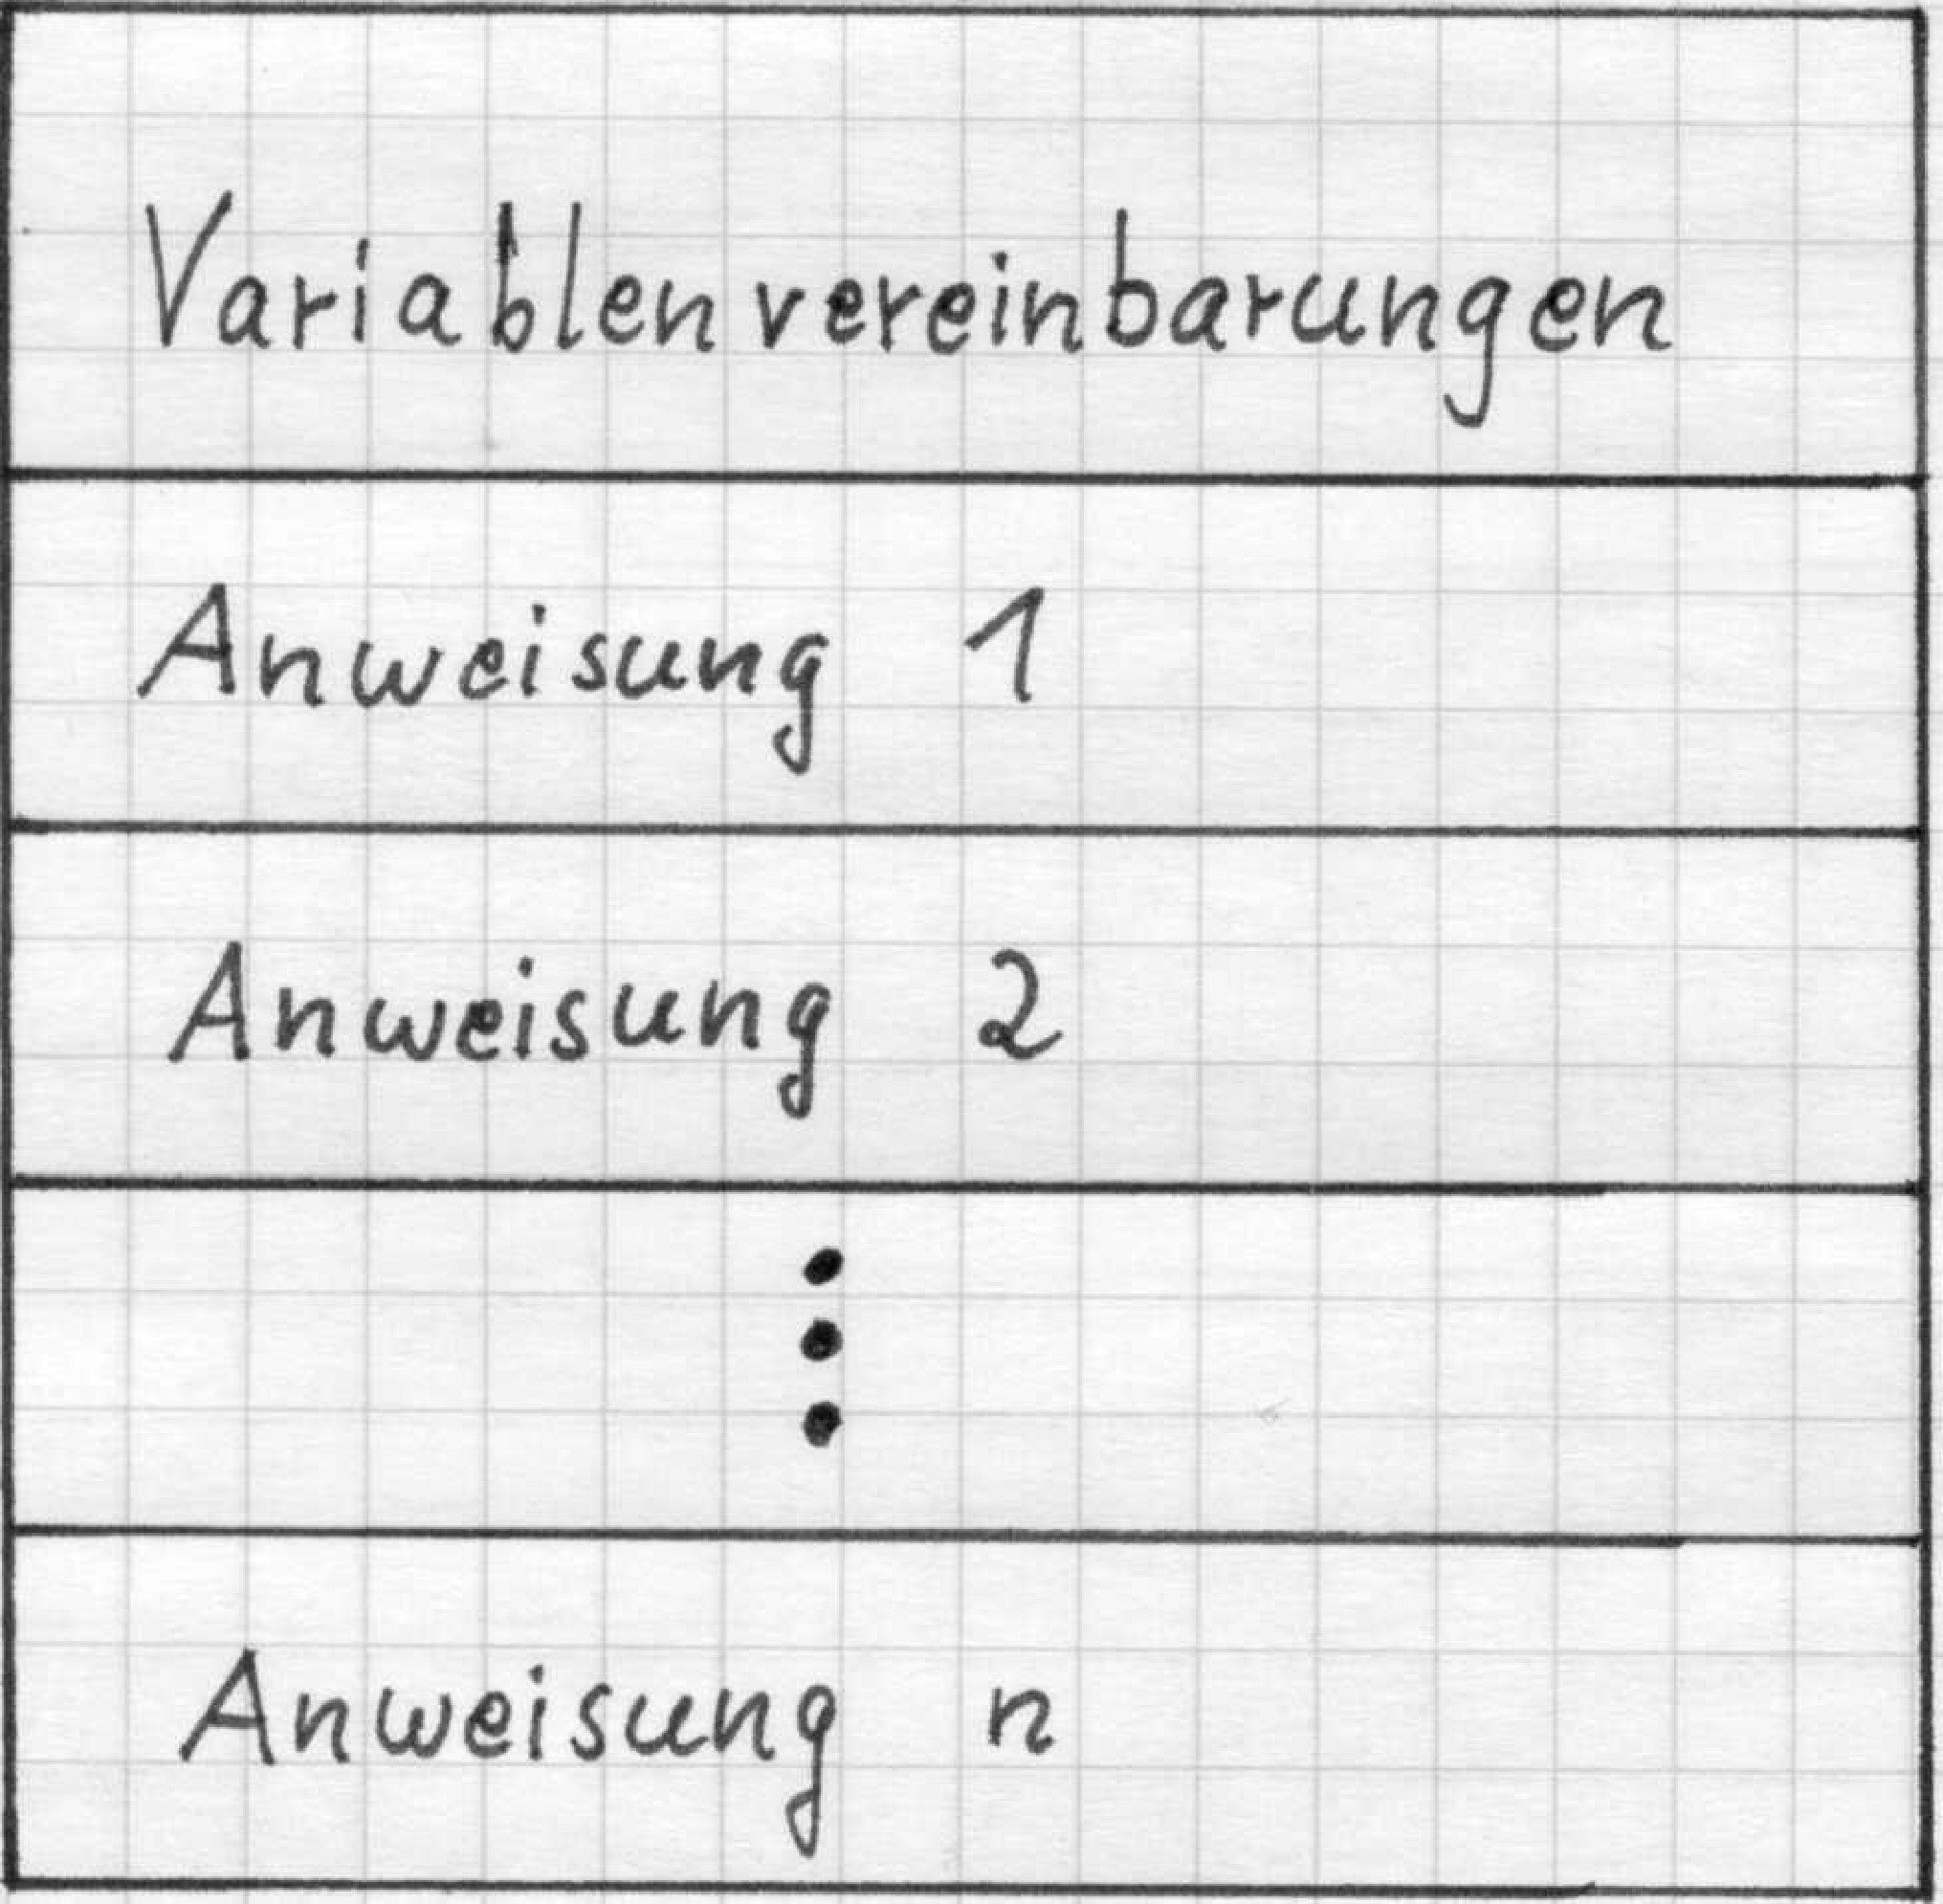
\includegraphics[scale=0.15]{GIF/p26}
%
\begin{itemize}
 \item
  In C {mu\ss} der Vereinbarungsteil dem Blockanfang direkt folgen.
  In C++ k"onnen mehrere Vereinbarungsteile im Block existieren, sie
  m"ussen nur vor der jeweiligen Erstbenutzung der Variablennamen stehen.
  Dies hat den Vorteil, da"s Variablen nur dort definiert (und initialisiert!!) werden m"ussen
  wo sie auch gebraucht werden.
 \item Der schlie{\ss}enden Klammer des Blockendes ``\}'' folgt kein
 	Semikolon.
 \item Ein Block kann stets anstelle einer Anweisung verwendet werden.
 \item Bl"ocke k"onnen beliebig ineinander  geschachtelt werden.
 \item Die in einem Block vereinbarten Variablen sind nur dort sichtbar,
 	d.h., au{\ss}erhalb des Blocks ist die Variable nicht existent
	(Lokalit"at). Umgekehrt kann auf Variablen des "ubergeordneten Blocks
	zugegriffen werden.\index{Block!Lokalit\"at}\index{scope}\index{Gültigkeitsbereich}
	%\exfile{Ex420.cpp}
\end{itemize}
\includecode[firstline=6]{Ex420.cpp}{Gültigkeitsbereich (scope) von Variablen}
%
Im Listing~\ref{lst:Ex420.cpp} tritt die Variable \texttt{i} sowohl im inneren
als auch im äußeren Block auf.
Dies nennt man \emph{shadow variable}, d.h., die innere Variable verdeckt die äußere.
Damit ist der Code schwerer zu verstehen und fehleranfälliger, ergo vermeiden Sie
shadow variables in Ihren Programmen.
Beim Gnu-Compiler warnt die Option \verb| -Wshadow | davor.
%
\section{Verzweigungen}
\label{p:4.3}
%
Die allgemeine Form der Verzweigungen (auch Alternative) ist
\index{Alternative}\index{Verzweigungen|see{Alternative}}
\index{if-then-else|see{Alternative}}

\mbox{}\hfill
\begin{minipage}[t]{0.6\textwidth}
\begin{verbatim}
if ( <logischer ausdruck> )
  <anweisung_A>
else
  <anweisung_B>
\end{verbatim}
\end{minipage}
\hfill\mbox{}

und z"ahlt ihrerseits wiederum als Anweisung. Der \verb|else|~-Zweig
kann weggelassen werden (einfache Alternative).

% \pagebreak[4]
\underline{Struktogramm}: \\
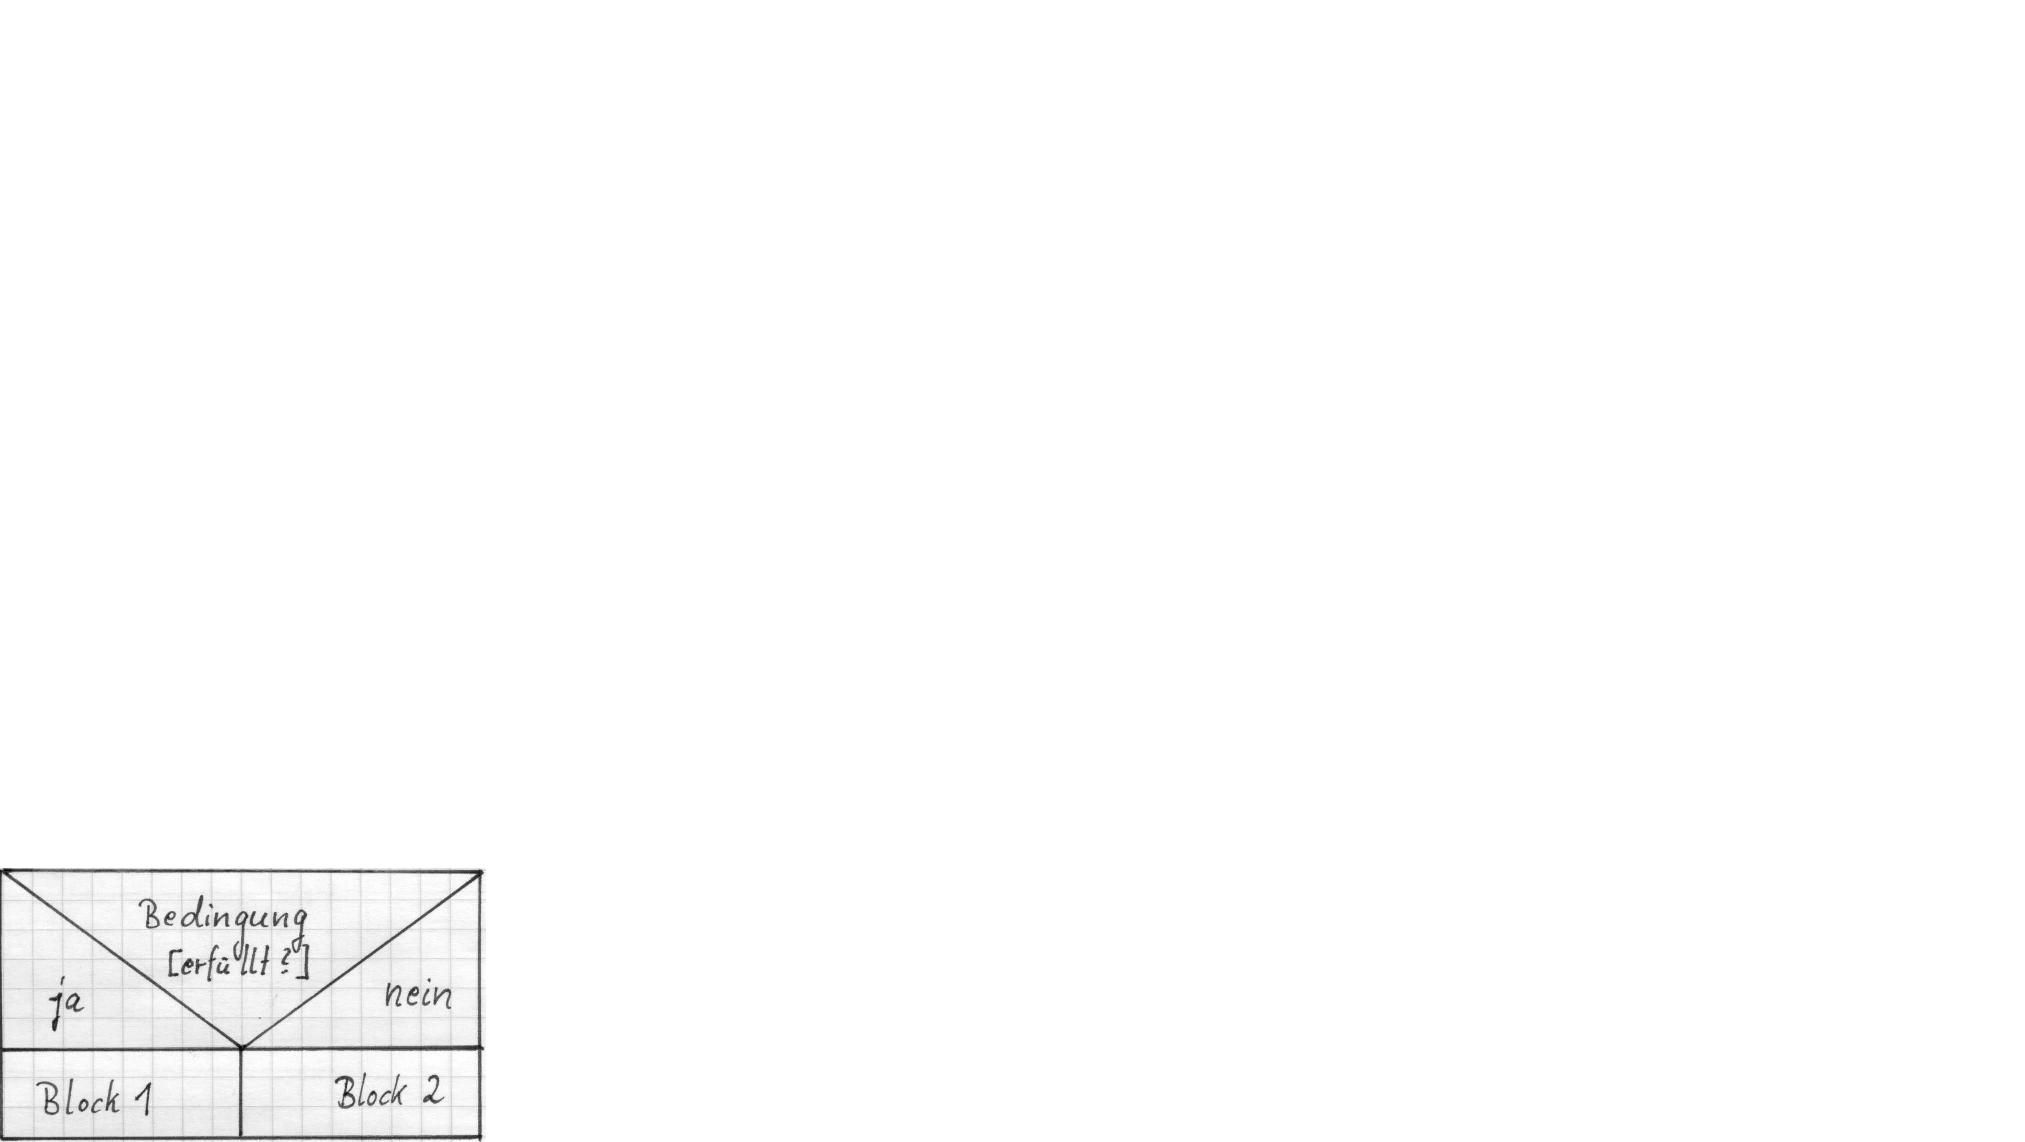
\includegraphics[scale=0.15]{GIF/p27.eps}
%

Wie so oft kann ein konkretes Problem auf verschiedene Weise
programmiert werden.
\\
\textbf{Beispiel}: Wir betrachten dazu die Berechnung der
Heaviside-Funktion\index{Heaviside}
$$
 y(x) = \begin{cases} 1 & \quad x \ge 0 \\ 0 & \quad x < 0 \end{cases}
$$
und stellen die folgenden vier Varianten der Implementierung vor.
%\exfile{Ex431.cpp}
\begin{enumerate}
	\renewcommand{\labelenumi}{\alph{enumi})}
	\item Setzen des Standardwertes kombiniert mit einer einfache Alternative,
	\item zweifache Alternative ohne Blöcke (da in jedem Zweig genau eine Anweisung steht),
	\item zweifache Alternative mit Blöcken (allgemeiner),
	\item mit dem Entscheidungsoperator.
	  Treten in einer zweifachen Alternative in jedem Zweig nur je eine
      Wertzuweisung zur selben Variablen auf (wie in Versionen b) und c)),
      dann kann der Entscheidungsoperator
      \\
     \centerline {\texttt{ <log.\  ausdruck> {\bf ?} <ausdruck\_A> {\bf :} <ausdruck\_B>  }}
\end{enumerate}
%
\includecode[firstline=7]{Ex431.cpp}{Vier Varianten um Heavisidefunktion zu implementieren}
%

\textbf{Beispiel}: Ein weiteres Beispiel ist die Berechnung
der Signum-Funktion (Vorzeichenfunktion)\index{Signum}
$$
 y(x) = \begin{cases} 1 & \quad x > 0 \\ 0 & \quad x = 0 \\ -1 & \quad x < 0 \end{cases}
$$
und wir stellen mehrere Varianten der Implementierung vor.
\bspfile{Ex432.cpp}
\label{bsp:sgn1}

\underline{Struktogramm}:\\
%
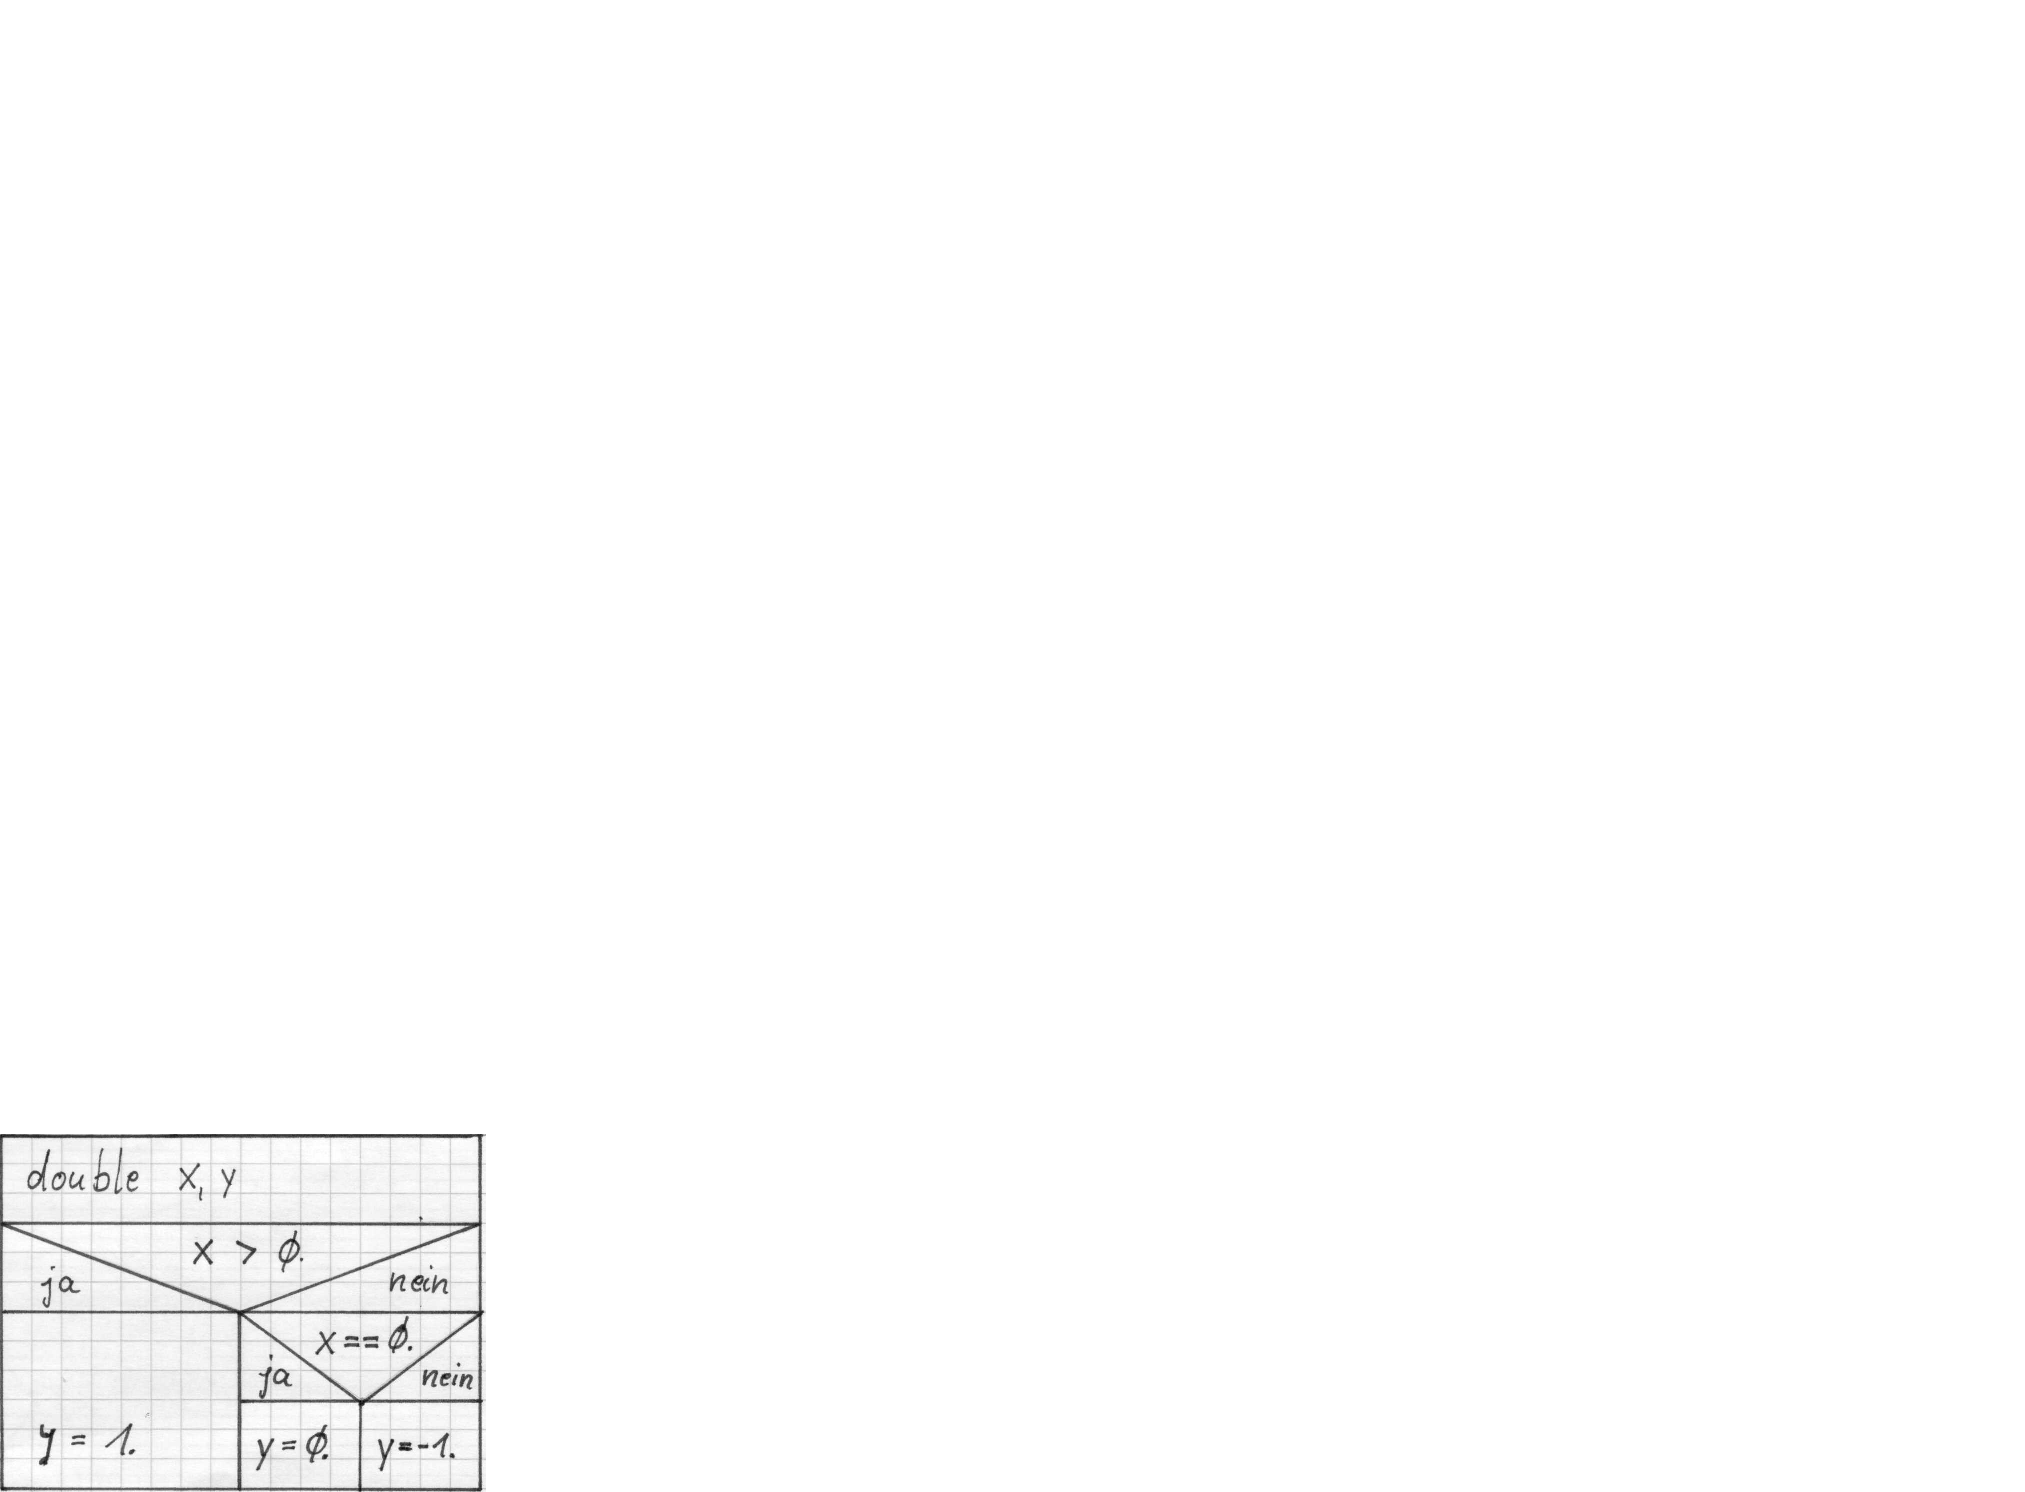
\includegraphics[scale=0.15]{GIF/p29.eps}
\\
%
Wir betrachten folgende Implementierungsvarianten:
\begin{enumerate}
	\renewcommand{\labelenumi}{\alph{enumi})}
	\item Schachtelung der Alternativen, d.h., der \verb|else|-Zweig enthält nochmals
	  eine Alternative.
	\item Falls der \verb|else|-Zweig nur aus einer
        weiteren \verb|if|-\verb|else|-Anweisung besteht, kann das  \verb|else| mit
        dem inneren \verb|if| zum \verb|elseif| kombiniert werden.
    \item Die Signumfunktion kann auch als Kombination von  zwei Heaviside-Funktionen
    ausgedrückt werden und damit als Kombination zweier Entscheidungsoperatoren
    implementiert werden (kurz und knapp, aber aus dem Code nur schwer zu verstehen).
\end{enumerate}
%
\includecode[firstline=7]{Ex432.cpp}{Drei Varianten der Signum-Funktion}
%

% \newpage
\begin{samepage}
Allgemein kann eine solche Mehrwegentscheidung als
\\[1ex]
\mbox{}\hfill
\begin{minipage}[t]{0.7\textwidth}
\begin{verbatim}
if ( <logischer ausdruck_1> )
  <anweisung_1>
else if ( <logischer ausdruck_2> )
  <anweisung_2>
        ...
else if ( <logischer ausdruck_(n-1)> )
  <anweisung_(n-1)>
else
  <anweisung_n>
\end{verbatim}
\end{minipage}
\hfill\mbox{}\label{mehrweg}
\\[1ex]
geschrieben werden, wobei der \verb|else|-Zweig wiederum optional ist.
\end{samepage}

\pagebreak{}
\begin{samepage}
\textbf{Beispiel}: Bestimmung von Minimum und Maximum
zweier einzugebender Zahlen.

\underline{Struktogramm}: \\
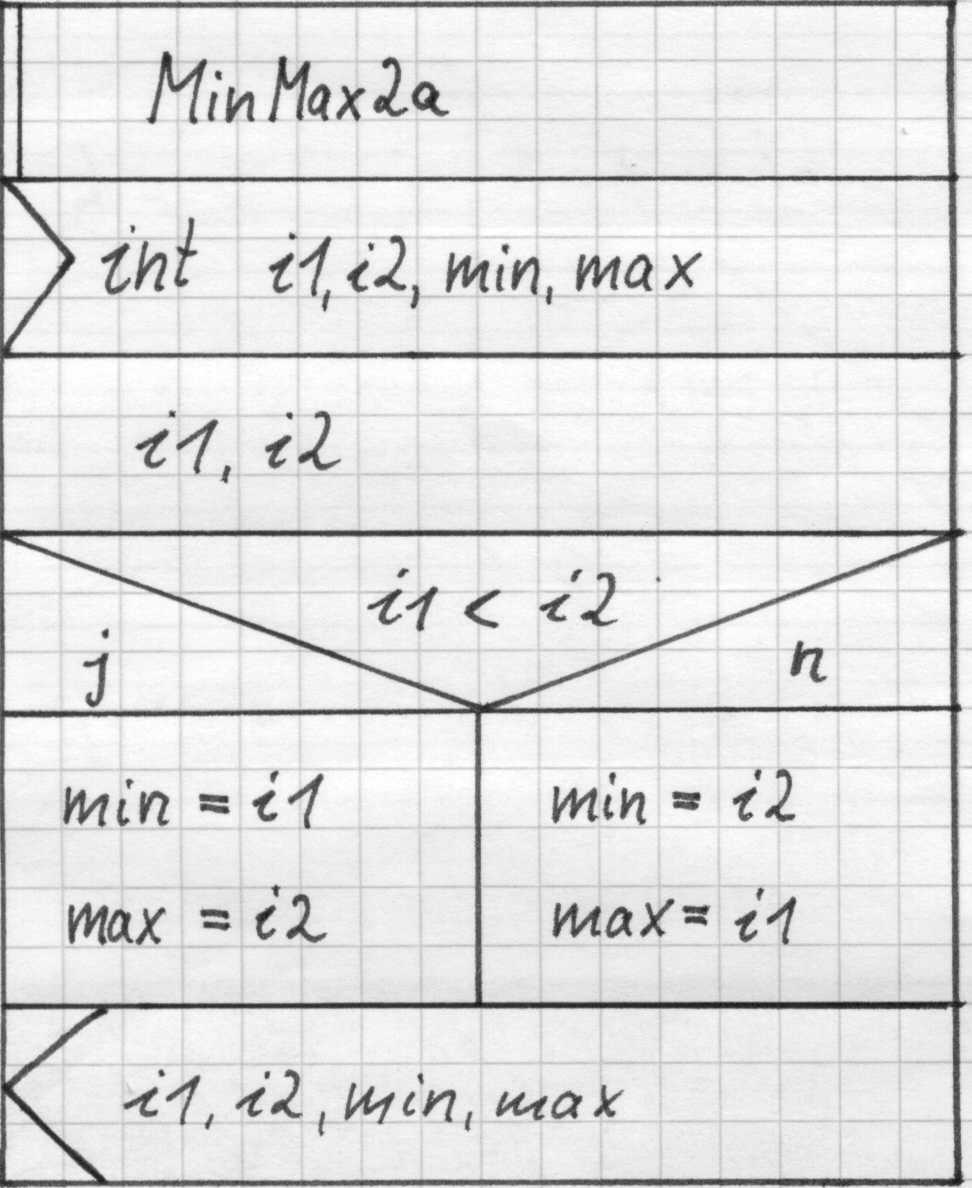
\includegraphics[scale=0.15]{GIF/p31a.eps}
\end{samepage}
\includecode[firstline=7]{Ex433.cpp}{Drei Varianten das Minimum und das Maximum zweier Zahlen zu bestimmen}
%
Die Funktionen \texttt{min} und \texttt{max} zur Bestimmung des Minimus/Maximums zweier Zahlen
sind in der STL (Standard Template Library) bereits implementiert,\index{STL}
somit lassen sich alle 3~Varianten auch durch
\verb| imax = max(i1,i2); imin = min(i1,i2); |
ausdrücken.

\pagebreak
\textbf{Beispiel}: Bestimmung des Minimums
dreier einzugebender Zahlen.
%\exfile{Ex434.cpp}

\underline{Struktogramm}: \\%[4cm]
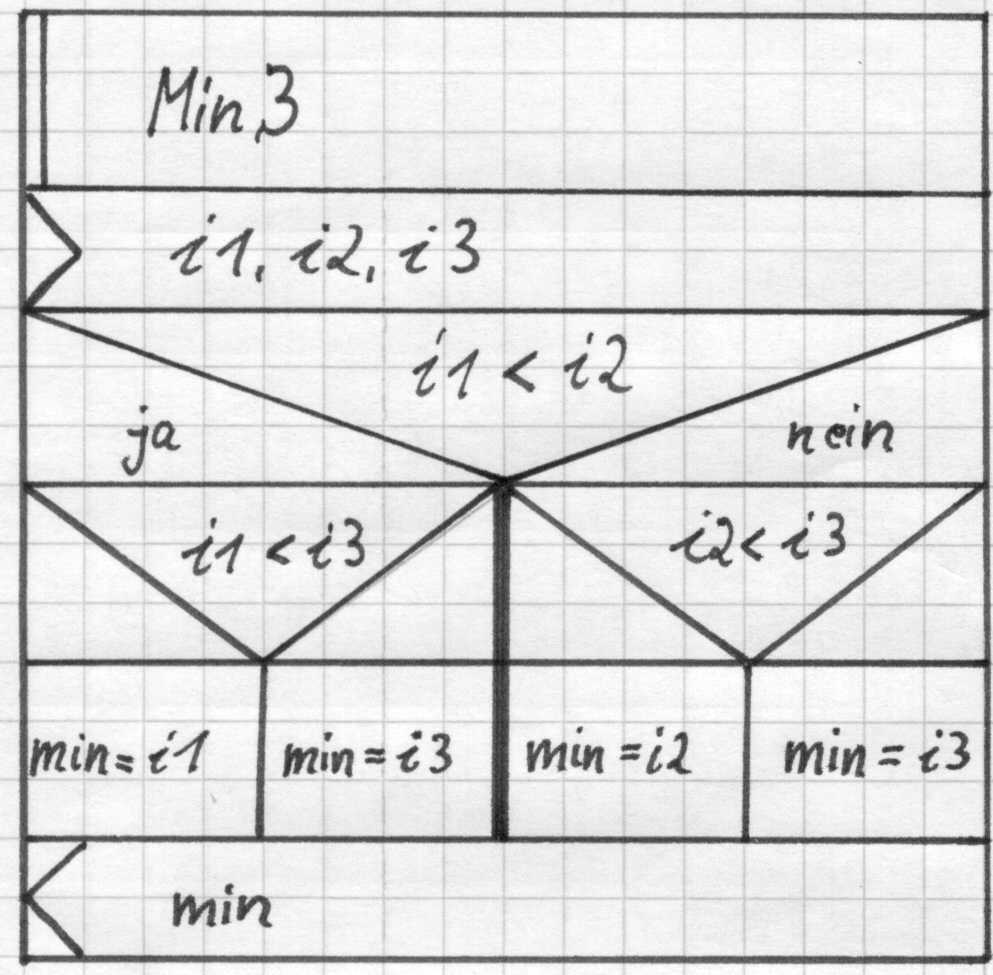
\includegraphics[scale=0.15]{GIF/p32.eps}
%
\includecode[firstline=7]{Ex434.cpp}{Varianten des Minimums dreier Zahlen}
%
%
%
\section[Der Z"ahlzyklus]{Der Z"ahlzyklus (\texttt{for}-Schleife)}
\label{p:4.4}
%
Beim Z"ahlzyklus steht die Anzahl der Zyklendurchl"aufe
\textbf{a-priori} fest, der Abbruchtest erfolgt vor dem Durchlauf eines Zyklus.
Die allgemeine Form ist
\index{Z\"ahlzyklus}\index{for-Schleife|see{Z\"ahlzyklus}}

\mbox{}\hfill
\begin{minipage}[t]{0.8\textwidth}
\begin{verbatim}
for (<ausdruck_1>; <ausdruck_2>; <ausdruck_3>)
  <anweisung>
\end{verbatim}
\end{minipage}
\hfill\mbox{}
%\newpage
Am besten sei der Z"ahlzyklus an einem Beipiel erl"autert.
%\newpage

\textbf{Beispiel}: Es ist die Summe der ersten 5 nat"urlichen
Zahlen zu berechnen: $\displaystyle isum = \sum_{i=1}^{5} i$.
%
\includecode[firstline=7]{Ex440.cpp}{Summe der ersten 5 natürlichen Zahlen}

Im obigen Programmbeispiel ist \verb|i| die
Laufvariable\index{Laufvariable} des Z"ahlzyklus,
welche mit \verb|i = 1| (\verb|<ausdruck_1>|) initialisiert, mit
\verb|i = i+1| (\verb|<ausdruck_3>|) weitergez"ahlt und in
\verb|i <= n| (\verb|<ausdruck_2>|) bzgl.\  der
oberen Grenze der Schleifendurchl"aufe getestet wird.
Im Schleifeninneren \verb|sum = sum + i;| (\verb|anweisung|) erfolgen die
eigentlichen Berechnungsschritte des Zyklus. Die  Summationsvariable
\verb|sum| {mu\ss} vor dem Eintritt in den Zyklus initialisiert werden.

Eine kompakte Version dieser Summationsschleife
(korrekt, aber sehr schlecht lesbar) w"are :
\\
\verb|for (isum = 0, int i = 1; i <= n; isum += i, ++i)|
\\
Man unterscheidet dabei zwischen dem Abschlu{\ss} einer Anweisung ``\verb|;|''
und dem Trennzeichen ``\verb|,|'' in einer Liste von Ausdr"ucken.
Diese Listen werden von links nach rechts abgearbeitet.

Der \verb|<ausdruck_2>| ist stets ein logischer Ausdruck
(\S~\ref{p:3.3}-\ref{p:3.4}) und \verb|<ausdruck_3>|
ist ein arithmetischer Ausdruck zur Manipulation der Laufvariablen,
z.B.\\[1ex]
\begin{minipage} {0.9\textwidth}
\begin{verbatim}
 ++i
 j = j-2
 j += 2
 x = x+h         // float-Typ
 k = 2*k         // Verdoppelung
 l = l/4         // Viertelung - Vorsicht bei Integer
\end{verbatim}
\end{minipage}

%\pagebreak[4]
\underline{Struktogramm}: \\
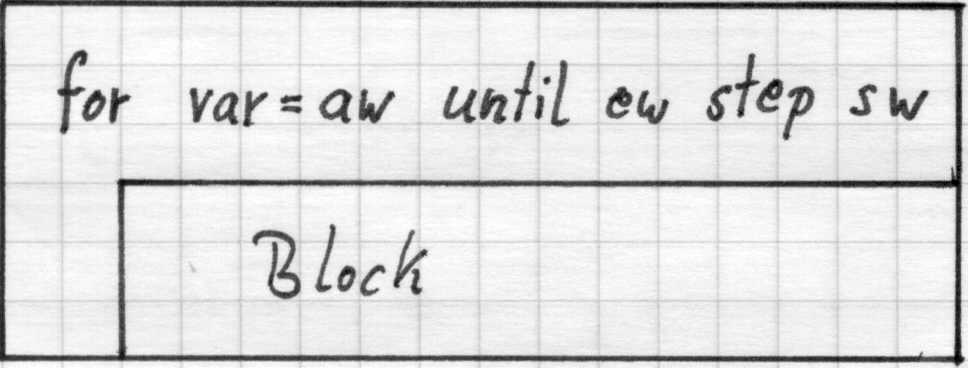
\includegraphics[scale=0.15]{GIF/p34.eps}
%
\begin{itemize}
 \item Die Laufvariable mu"s eine einfache Variable aus \S~\ref{p:2.2}
 	sein, z.B., \verb|int| oder \verb|double|,\index{Laufvariable}
	oder ein Iterator~\S~\ref{p:6.3} (auch Pointer).
 \item Vorsicht bei Verwendung von Gleitkommazahlen
 (\verb|float|, \verb|double|) als\bspfile{Loop_Float.cpp}
 Laufvariable.\index{Laufvariable!Gleitkommazahl}\index{Gleitkommazahl!Laufvariable}
 Dort ist der korrekte Abbruchtest wegen der internen Zahldarstellung
 u.U.\  nicht einfach zu realisieren.\index{Z\"ahlzyklus!Abbruchtest}
\end{itemize}


\begin{minipage}[c]{0.4\textwidth}
\textbf{Beispiel}:
Es sei die Doppelsumme
$$
  \text{sum} = \sum_{k=1}^n \underbrace{\sum_{i=1}^k \frac{1}{i^2}}_{t_k}
  =  \sum_{k=1}^n t_k
$$
f"ur einzugebende $n$ zu berechnen.\\
\textbf{Hinweis:} F"ur die innere Summe gilt $t_k = t_{k-1}+1/k^2$
f"ur $k=1,\ldots,n$ mit $t_0 = 0$. Dadurch f"allt diese kostspielige
Summation weg wodurch der gesamte Code signifikant schneller wird
%% \htmladdnormallink{\textit{Ex442fast.cpp}}{\url{../../Examples/Ex442fast.cpp}}).
%%(\htmladdnormallink{\textit{Ex442fast.cpp}}{../../Examples/Ex442fast.cpp}).%
\footnote{Andere M"oglichkeit:
Vertauschen der Summationen $\sum_{i=1}^n \sum_{k=i}^n \frac{1}{i^2}
 =  \sum_{i=1}^n  \frac{n-i+1}{i^2}$ [A. Reinhart]}
\end{minipage}\bspfile{Ex442fast.cpp}
%
%
% weitere Variante: Hr. Andreas Reinhart
%
% vertauschen der Summen:
% $
% \text{sum} = \sum_{i=1}^n \sum_{k=i}^n \frac{1}{i^2}
% =  \sum_{i=1}^n  \frac{n-i+1}{i^2}
% $
%
%
\hfill
\begin{minipage}{0.5\textwidth}
\underline{Struktogramm}: \\
%
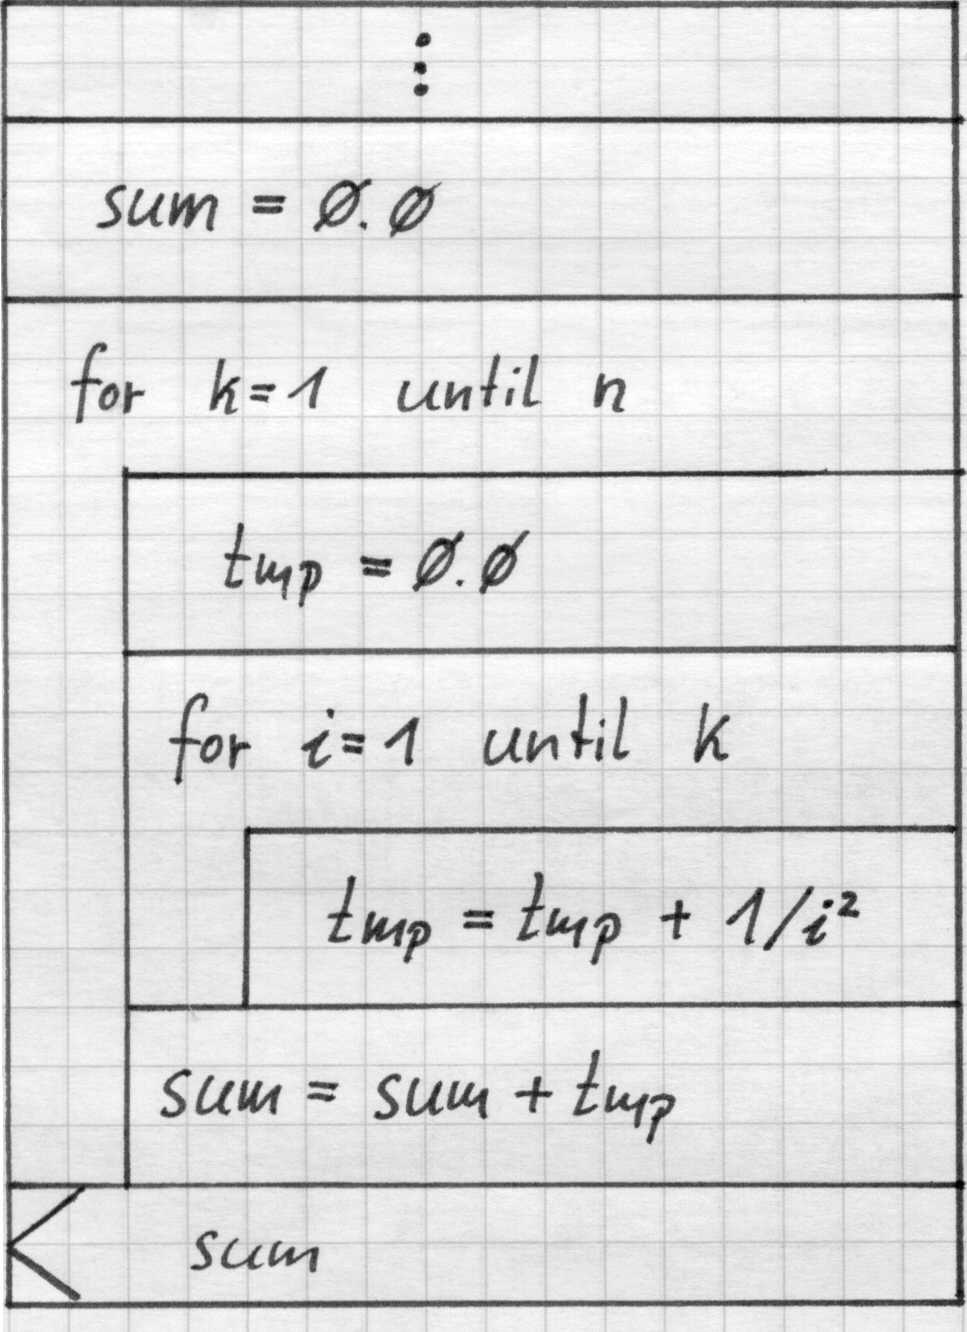
\includegraphics[scale=0.15]{GIF/p35.eps}
\end{minipage}
%
\includecode[firstline=7]{Ex442.cpp}{Geschachtelte Zählzyklen}
%

Weitere einfache \textbf{Beispiele} berechnen die Summe der
ersten geraden nat"urlichen Zahlen
\bspfile{Ex443.cpp}
und das Z"ahlen eines CountDowns.
\bspfile{Ex444.cpp}

%
%				woanders einbauen ?
%
Die folgenden Beispiele verdeutlichen die Problematik der
begrenzten Genauigkeit von Gleitkommazahlen in Verbindung
mit Zyklen und einige Tips zu deren Umgehung.\index{Gleitkommazahl!Genauigkeit}

% %\pagebreak
% \textbf{Beispiel:} Ausgabe der St"utzpunkte $x_i$ des Intervalls~$[0,1]$,
% welches in $n$~gleichgro"se Teilintervalle zerlegt wird, d.h.,
% \bspfile{Loop\_Float.cpp}
% $$
%  x_i = i \cdot h \quad,\;i=0,\ldots,n\qquad\text{mit } h = \frac{1-0}{n}
% $$
% \underline{Struktogramm}: \\
% \begin{latexonly}
% \special{psfile=GIF/p36b.eps.gz
% 	 hscale=15 vscale=15
% 	 voffset=-90
% 	}
% \\[3cm]
% \end{latexonly}
% \htmladdimg{p36b_4.jpg}{}
\begin{minipage}{0.4\textwidth}
\underline{Struktogramm}: \\
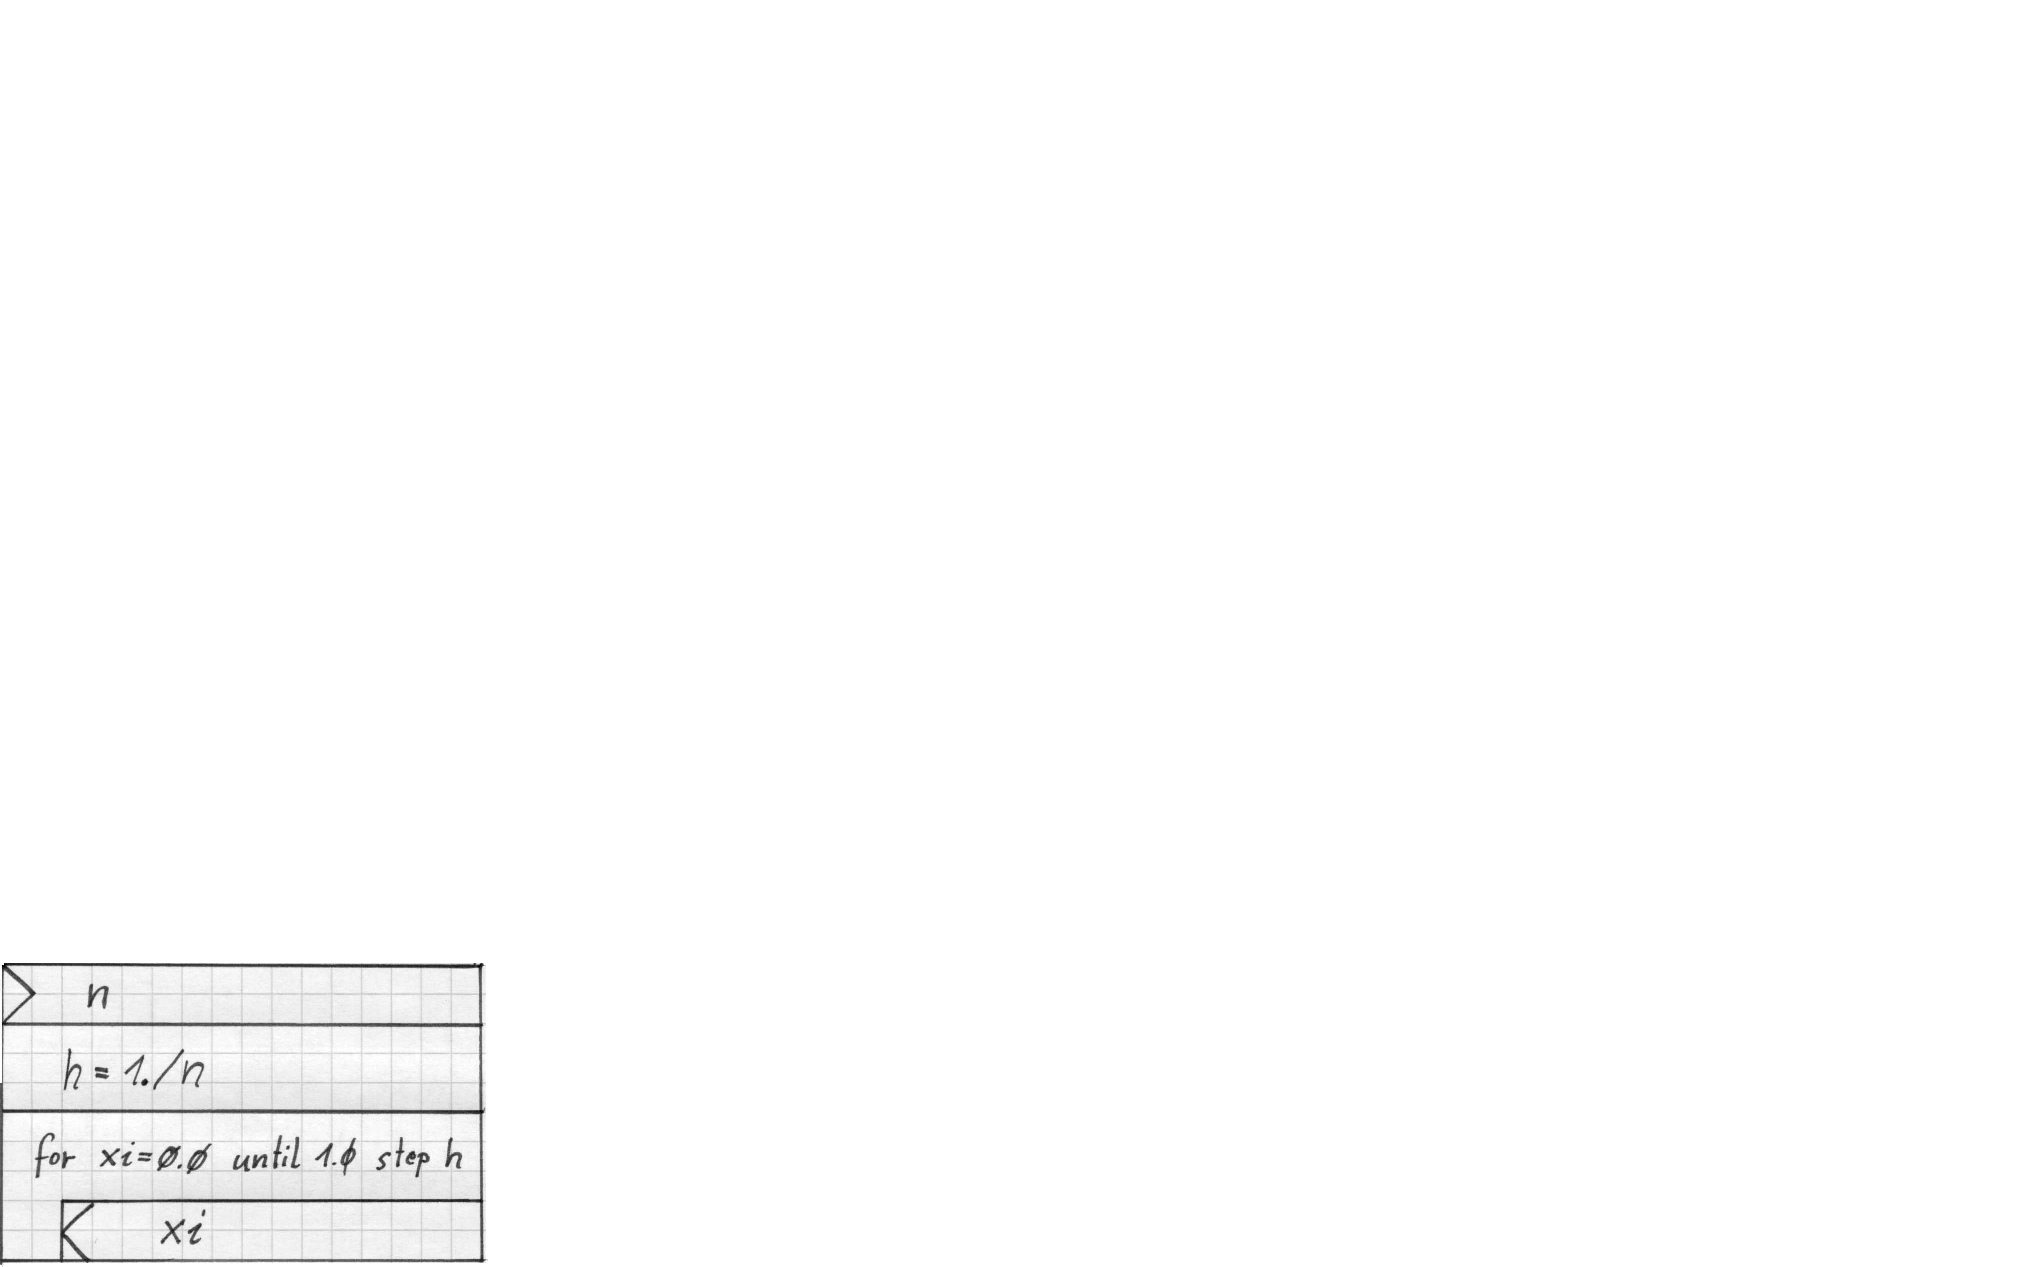
\includegraphics[scale=0.15]{GIF/p36b.eps}
\end{minipage}
%
\begin{minipage}{0.5\textwidth}
\textbf{Beispiel:} Ausgabe der St"utzpunkte $x_i$ des Intervalls~$[0,1]$,
welches in $n$~gleichgro"se Teilintervalle zerlegt wird, d.h.,
$$
 x_i = i \cdot h \quad,\;i=0,\ldots,n\qquad\text{mit } h = \frac{1-0}{n}
$$
\end{minipage}\bspfile{Loop\_Float.cpp}
%
% \pagebreak[4]
\includecode[linerange={7-8,11-17,33-38,41-42}]{Loop_Float.cpp}
{Aufpassen bei Zählzyklen mit Gleikommagröße als Laufvariable}
%
Da Gleitkommazahlen nur eine limitierte Anzahl g"ultiger Ziffern besitzen,
kann es (oft) passieren, da"s der letzte Knoten $x_n$ nicht
ausgegeben wird. Nur f"ur $n=2^k\;,\,k\in {\mathbb{N}}\;,\;k<32$ kann in unserem
Beispiel eine korrekte Abarbeitung des Z"ahlzyklus garantiert werden.
Auswege sind: 
\begin{enumerate}
 \item "Anderung des Abbruchtests in \verb| xi <= xe + h/2.0 |, jedoch
 	ist $x_n$ immer noch fehlerbehaftet. \\[1ex]
%
\begin{minipage} {0.5\textwidth}
\begin{verbatim}
 for (xi = xa; xi <= xe + h/2.0; xi += h)
   {
    cout << xi << endl;
   }
\end{verbatim}
\end{minipage}
 \item Besser ist ein Zählzyklus mit einer \verb|int|-Laufvariable wodurch
    die Werte $x_{i} = i \cdot h$ für große~$i$ genauer sind als in Variante~1.
    \\[2ex]
\nopagebreak
\begin{minipage} {0.5\textwidth}
\begin{verbatim}
 for (i = 0; i <= n; ++i)
   {
    xi = xa + i*h;
    cout << xi << endl;
   }
\end{verbatim}
\end{minipage}
\end{enumerate}

%\pagebreak
Die gemeinsame Summation kleinerer und gr"o"serer Zahlen kann ebenfalls zu
Ungenauigkeiten f"uhren. Im \textbf{Beispiel} wird
die Summe $s1:=\sum\limits_{i=1}^{n} 1/i^2$ mit
der (theoretisch identischen) Summe $s2:=\sum\limits_{i=n}^{1} 1/i^2$
f"ur gro"se $n$ ($65.000$, $650.000$) verglichen.
%
\includecode[linerange={7-8,10-13,21-29,33-40,51-52}]{Reihe.cpp}
{Auslöschung bei Summation kleiner Zahlen}
%
\index{cmath!ceil()}\index{numeric\_limits!epsilon}\index{numeric\_limits}

Das numerische Resultat in $s2$ ist genauer, da dort zuerst alle kleinen
Zahlen addiert werden, welche bei $s1$
wegen der beschr"ankten Anzahl g"ultiger Ziffern
keinen Beitrag zur Summation mehr liefern k"onnen.
Gleichzeitig ist zu beachten, da"s die Berechnung
von \verb| 1.0/(i*i) | in einem "Uberlauf endet, da \verb| i*i |
nicht mehr in \verb|int|-Zahlen darstellbar ist.
Dagegen erfolgt die Berechnung von \verb| 1.0/i/i |
vollst"andig im Bereich der Gleitkommazahlen.\index{Gleitkommazahl!\"Uberlauf}
%
%
%
\pagebreak
\section[Abweisender Zyklus]{Abweisender Zyklus (\texttt{while}-Schleife)}
\label{p:4.5}
%
Beim abweisenden Zyklus steht die Anzahl der Durchl"aufe nicht
a-priori fest, der Abbruchtest erfolgt \textbf{vor} dem Durchlauf eines Zyklus.
\index{abweisender Zyklus}\index{while-Schleife|see{abweisender Zyklus}}
\index{abweisender Zyklus!Abbruchtest}

% Die allgemeine Form ist
% 
% \mbox{}\hfill
% \begin{minipage}[t]{0.6\textwidth}
% \begin{verbatim}
% while (<logischer ausdruck>)
%   <anweisung>
% \end{verbatim}
% \end{minipage}
% \hfill\mbox{}

\begin{minipage}[t]{0.5\textwidth}
Die allgemeine Form ist\\[1ex]
\phantom{XXX}\verb|while (<logischer ausdruck>)| \\
\phantom{XXX}\verb|    <anweisung>|
\end{minipage}
\begin{minipage}[t]{0.4\textwidth}
\underline{Struktogramm}: %\\
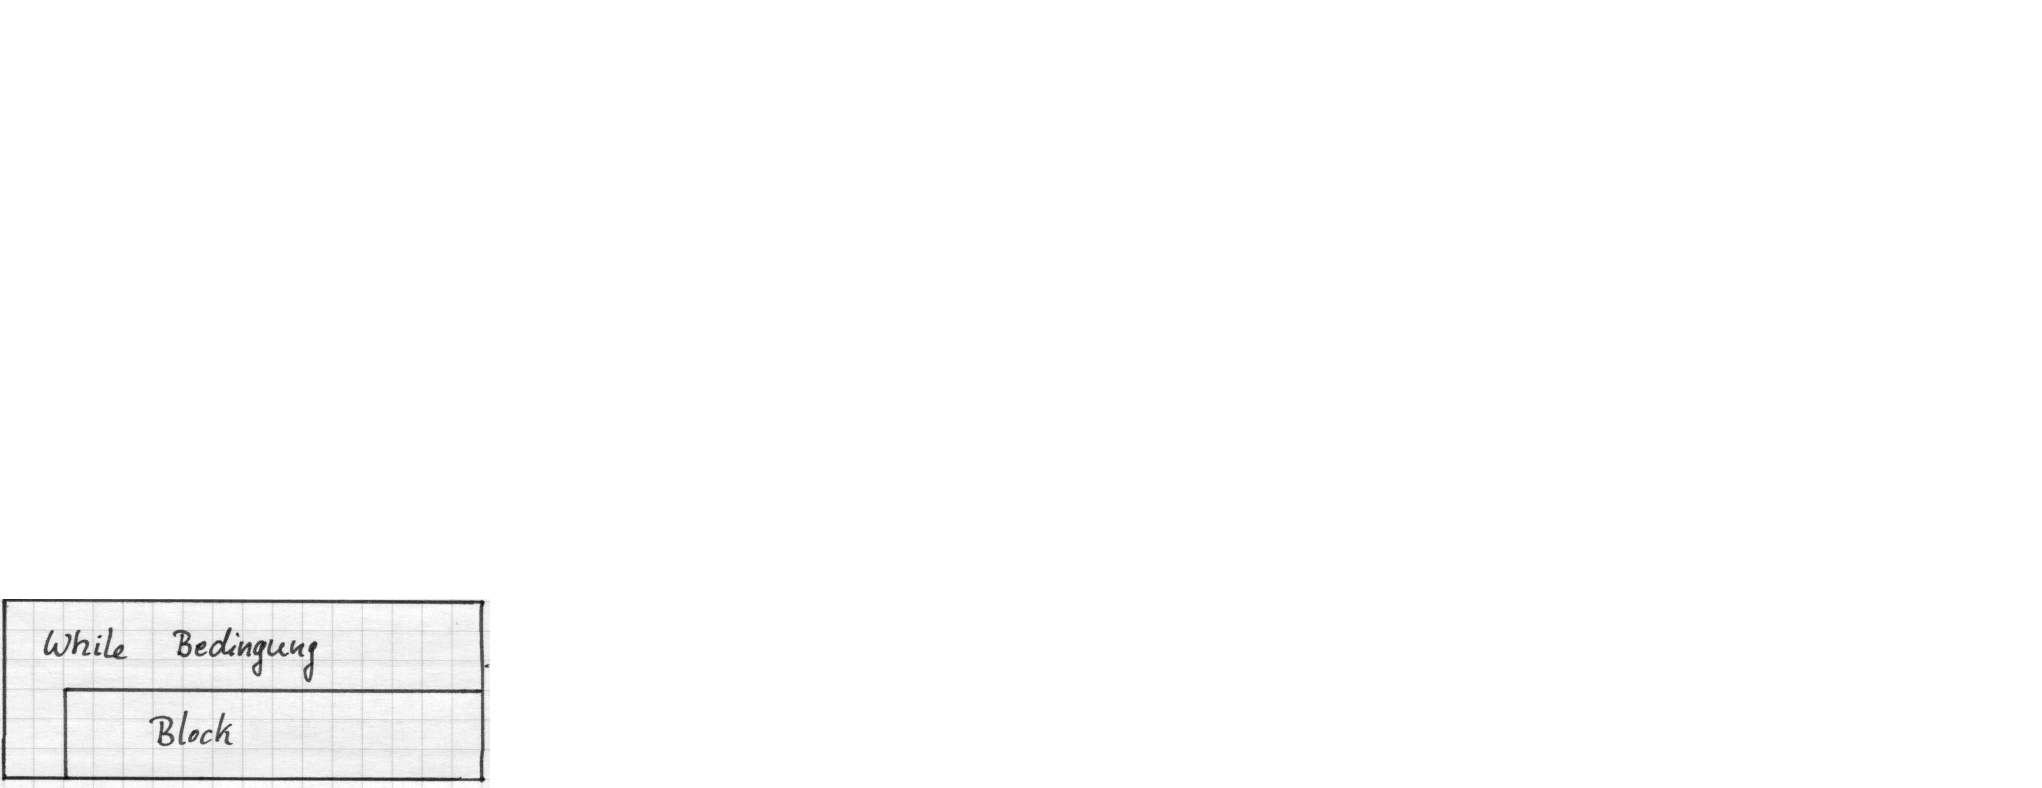
\includegraphics[scale=0.15]{GIF/p39.eps}
\end{minipage}

\textbf{Beispiel}: Bestimme den aufgerundeten Binärlogarithmus (Basis~2)
einer einzulesenden Zahl.\index{Bin\"arlogarithmus}
\includecode[linerange={7-11,13-22,25-26}]{Ex450.cpp}{Ganzzahliger Anteil des Binärlogarithmus einer Zahl}
%
% 
% \underline{Struktogramm}: %\\
% % \begin{latexonly}
% %   \special{psfile=GIF/p39.eps.gz
% % 	   hscale=15 vscale=15
% % 	   voffset=-55
% % 	  }
% %   \vspace{2cm}
% % \end{latexonly}
% % \begin{htmlonly} \\ \htmladdimg{p39_4.jpg}{}  \end{htmlonly}
% 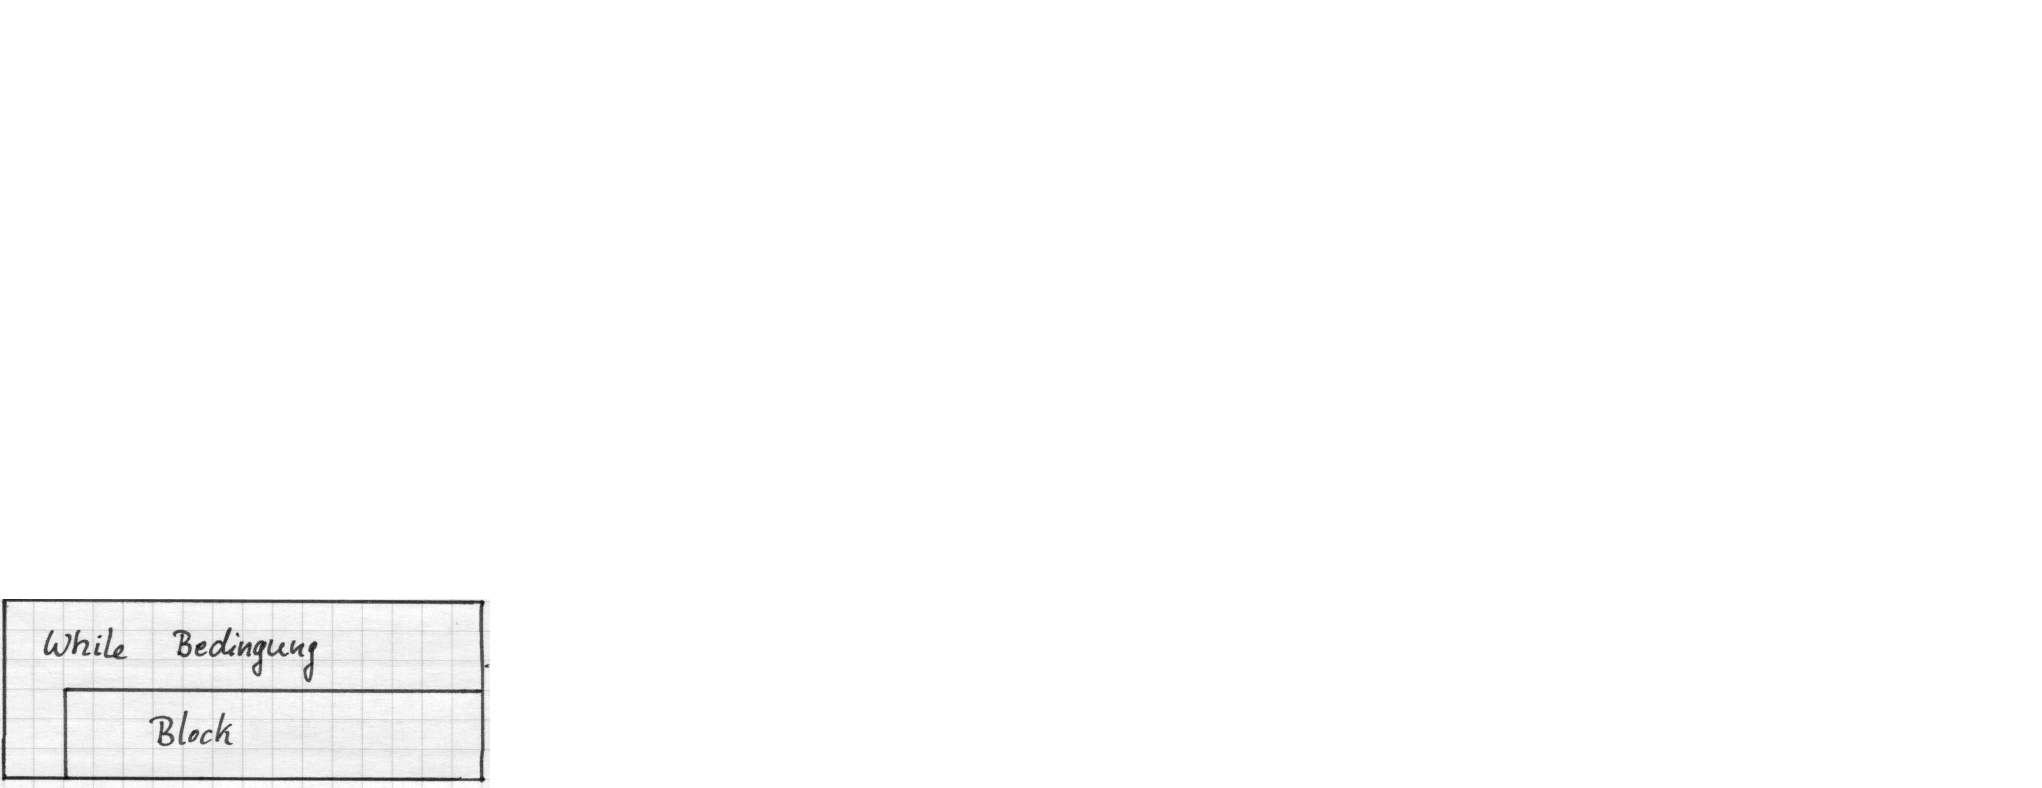
\includegraphics[scale=0.15]{GIF/p39.eps}


\underline{Bemerkung:} Falls der allererste Test im abweisenden Zyklus \texttt{false}
ergibt, dann wird der Anweisungsblock im Zyklusinneren
nie ausgef"uhrt (der Zyklus wird abgewiesen).

%
%
\section[Nichtabweisender Zyklus]{Nichtabweisender Zyklus (\texttt{do}-\texttt{while}-Schleife)}
\label{p:4.6}
%
Beim nichtabweisenden Zyklus steht die Anzahl der Durchl"aufe nicht
a-priori fest, der Abbruchtest erfolgt \textbf{nach} dem Durchlauf
eines Zyklus. Somit durchl"auft der nichtabweisende Zyklus mindestens
einmal die Anweisungen im Zyklusinneren.
\index{nichtabweisender Zyklus}\index{do-while-Schleife|see{nichtabweisender Zyklus}}
\index{nichtabweisender Zyklus!Abbruchtest}

% Die allgemeine Form ist
% 
% \mbox{}\hfill
% \begin{minipage}[t]{0.6\textwidth}
% \begin{verbatim}
% do
%   <anweisung>
% while (<logischer ausdruck>) ;
% \end{verbatim}
% \end{minipage}
% \hfill\mbox{}
% 
% \underline{Struktogramm}: \\
% % \begin{latexonly}
% %  \special{psfile=GIF/p40.eps.gz
% % 	  hscale=15 vscale=15
% % 	  voffset=-55
% % 	 }
% %  \vspace{2cm}
% % \end{latexonly}
% % \htmladdimg{p40_4.jpg}{}
% 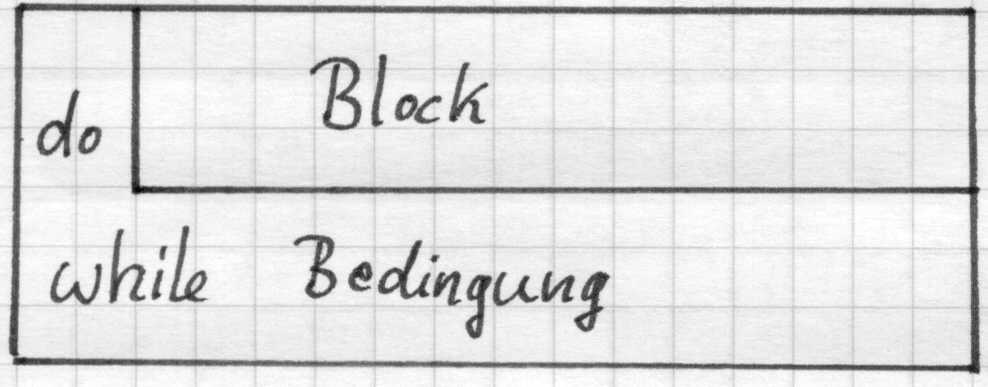
\includegraphics[scale=0.15]{GIF/p40.eps}

\begin{minipage}[t]{0.5\textwidth}
Die allgemeine Form ist\\[1ex]
\phantom{XXX}\verb|do| \\
\phantom{XXX}\verb|    <anweisung>|\\
\phantom{XXX}\verb|while (<logischer ausdruck>) ;|
\end{minipage}
\begin{minipage}[t]{0.4\textwidth}
\underline{Struktogramm}: %\\
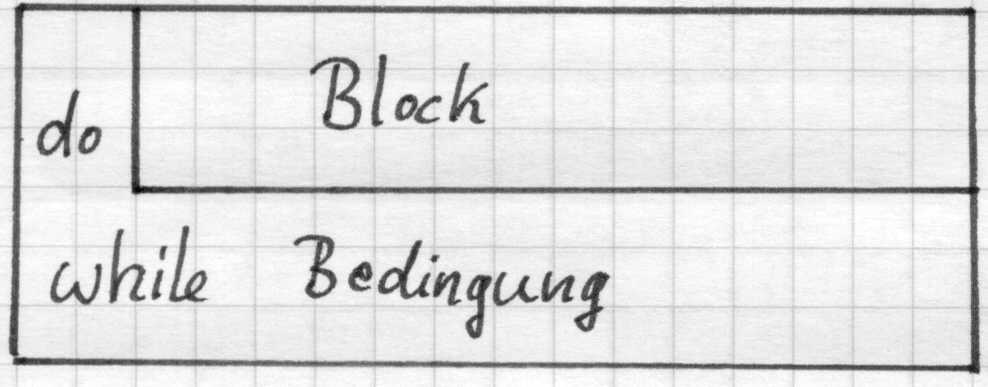
\includegraphics[scale=0.15]{GIF/p40.eps}
\end{minipage}



\textbf{Beispiel}: Es wird solange ein Zeichen von der
Tastatur eingelesen, bis ein \textit{x} eingegeben wird.
\includecode[linerange={7-19,22-23}]{Ex460.cpp}{Zeicheneingabe bis zum Exit-Zeichen \texttt{x}}
%

Betrachten wir ein etwas anspruchsvolleres \textbf{Beispiel}, und zwar soll
die L"osung von $\sin(x) = x/2$ mit $x\in(0,\pi)$ bestimmt werden.
Hierzu betrachtet man die "aquivalente Nullstellenaufgabe: Bestimme
die Nullstelle $x_0\in(0,\pi)$ der Funktion
$f(x) := \sin(x) - x/2 = 0$\enspace.\index{Nullstellen}
\label{bsp:bisection0}
\\
\underline{Analytisch:} Kein praktikabler L"osungsweg vorhanden.
\\
\underline{Graphisch:} Die Funktion $f(x)$ wir graphisch dargestellt
und das L"osungsintervall manuell verkleinert (halbiert).
Diesen Proze"s setzt man so lange fort, bis $x_0$ genau genug,
d.h., auf eine vorbestimmte Anzahl von Stellen genau,
bestimmt werden kann. \\[0.5ex]
% \epsfig{file=Ex46202.eps,height=4cm} \hfill
% 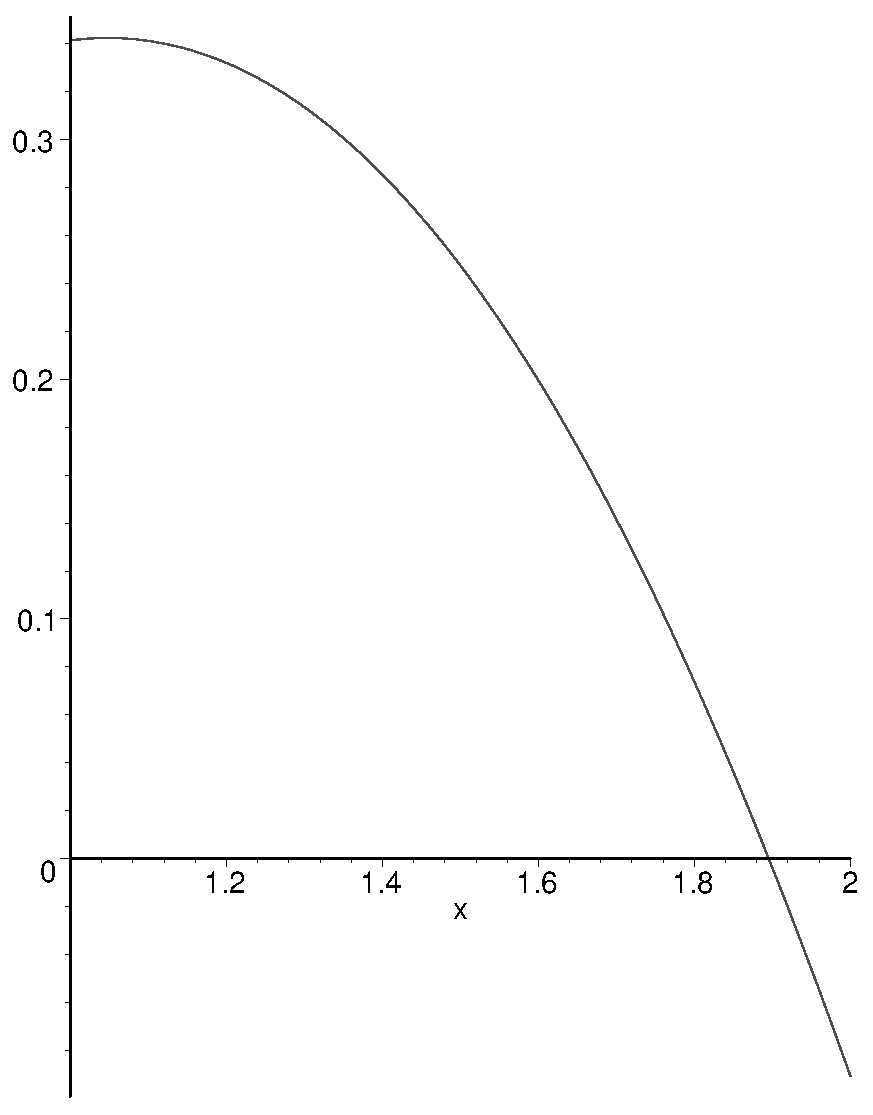
\epsfig{file=Ex46203.eps,height=4cm} \hfill
% 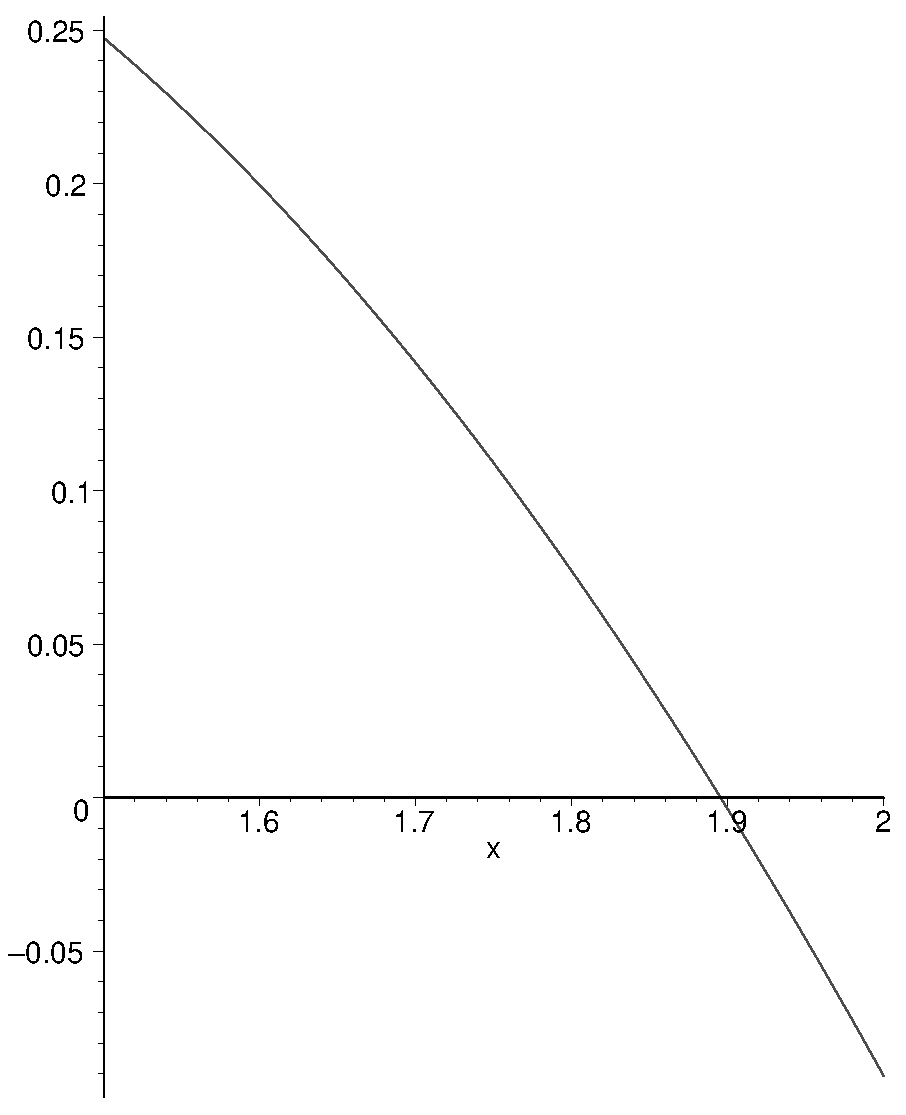
\epsfig{file=Ex46204.eps,height=4cm}
%
\includegraphics[height=4cm]{Ex46202.eps} \hfill
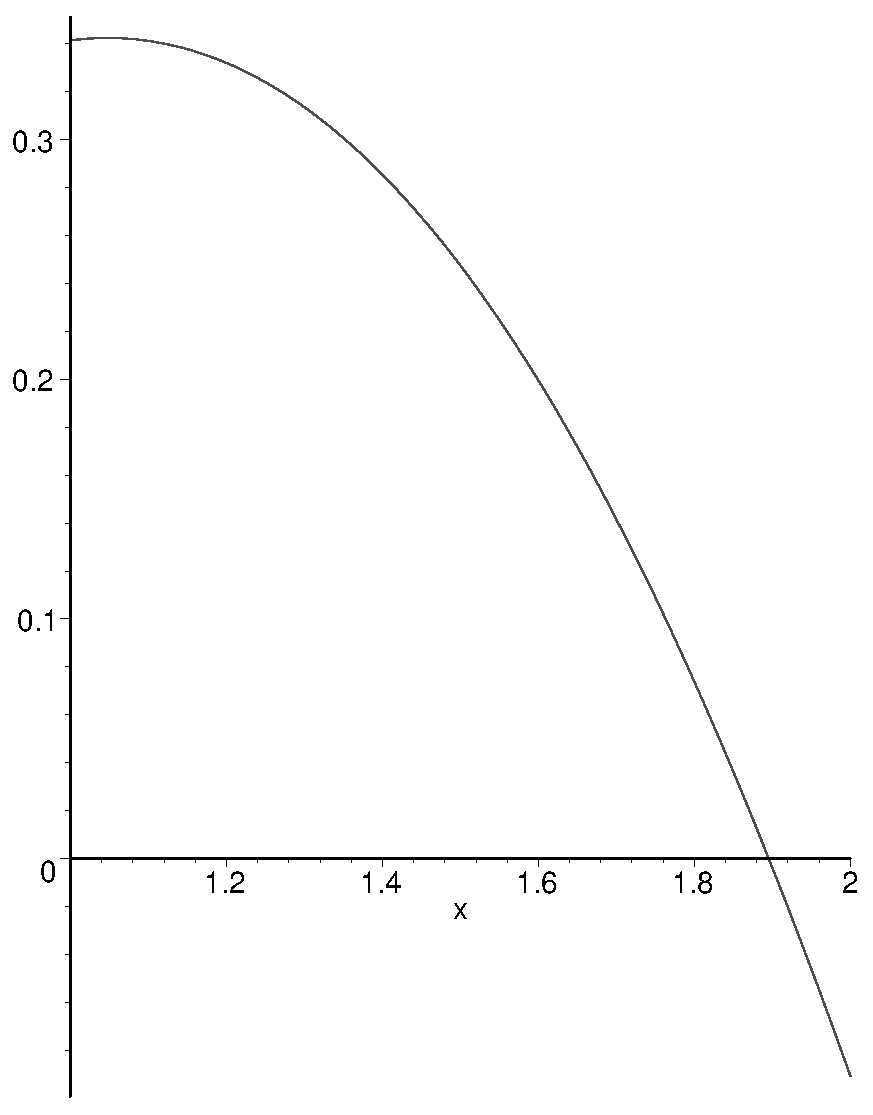
\includegraphics[height=4cm]{Ex46203.eps} \hfill
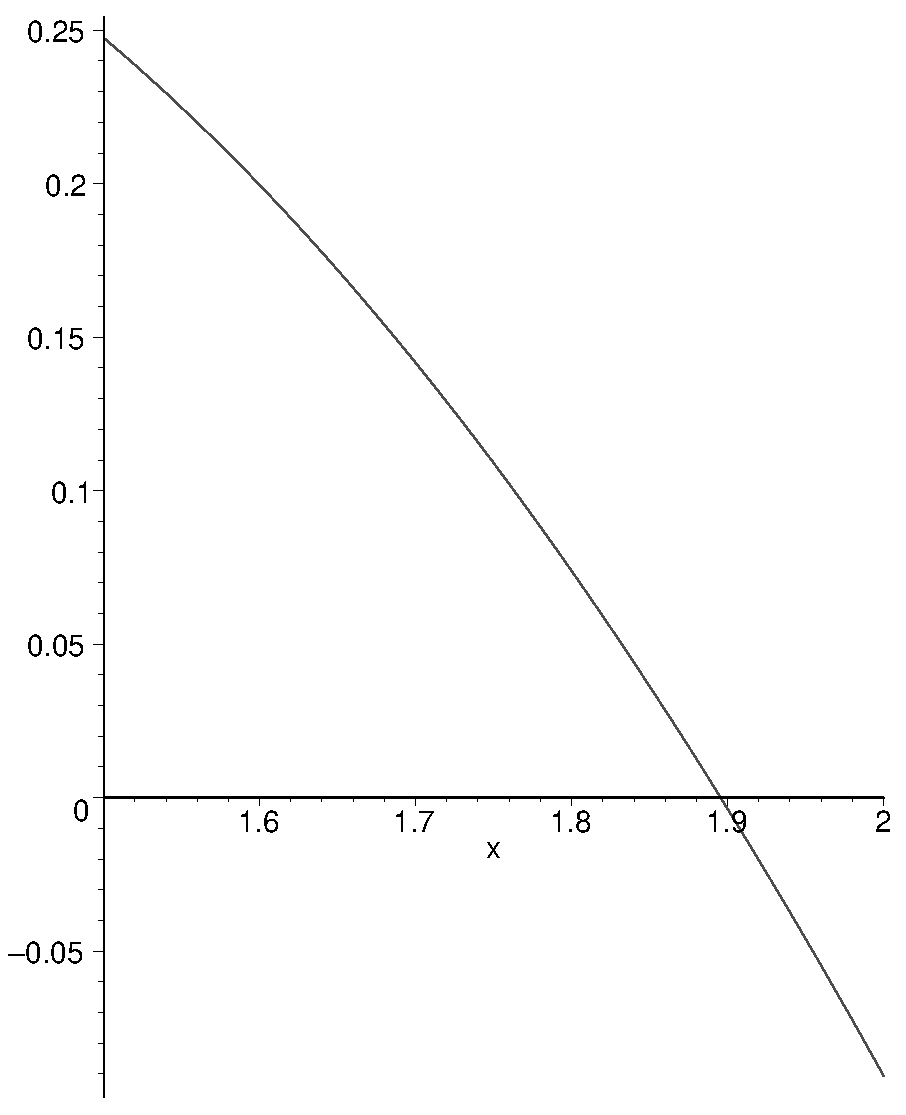
\includegraphics[height=4cm]{Ex46204.eps}
\\[0.5ex]
\underline{Numerisch:} Obiges, graphisches Verfahren kann auf ein
rein numerisches Verfahren im Computer "ubertragen werden
(der \textit{MAPLE}-Aufruf \texttt{fsolve(sin(x)=x/2,x=0.1..3}
liefert als N"aherungsergebnis $x_0 = 1.895494267$\enspace).
\bspfile{Ex462.mws}
Wir entwickeln ein Programm zur Bestimmung der Nullstelle
von $f(x) := \sin(x) - x/2$ im Intervall $[a,b]$
mittels Intervallhalbierung, wobei zur Vereinfachung
angenommen wird, da"s $f(a) >0$ und $f(b)<0$ ist.
Der Mittelpunkt des Intervalls sei mit $c:=(a+b)/2$ bezeichnet.
Dann k"onnen wir "uber die L"osung Folgendes aussagen:
$
\begin{cases}
 x_0 := c 	& \text{falls } f(c) = 0 \\
 x_0 \in [c,b]	& \text{falls } f(c) > 0 \\
 x_0 \in [a,c]	& \text{falls } f(c) < 0
\end{cases}
$\enspace.
%
Durch Redefinition der Intervallgrenzen $a$ und $b$ kann die
Nullstellensuche auf das kleinere (halbierte) Intervall
reduziert werden. Wir demonstrieren die Umsetzung mittels
eines nichtabweisenden Zyklus.
\bspfile{Ex462.cpp}

% 
% \underline{Struktogramm}: \\
% % \begin{latexonly}
% %   \special{psfile=GIF/p41a.eps.gz
% % 	   hscale=20 vscale=20
% % 	   voffset=-180
% % 	  }
% %   \vspace{6.3cm}
% % \end{latexonly}
% % \htmladdimg{p41a_4.jpg}{}
% 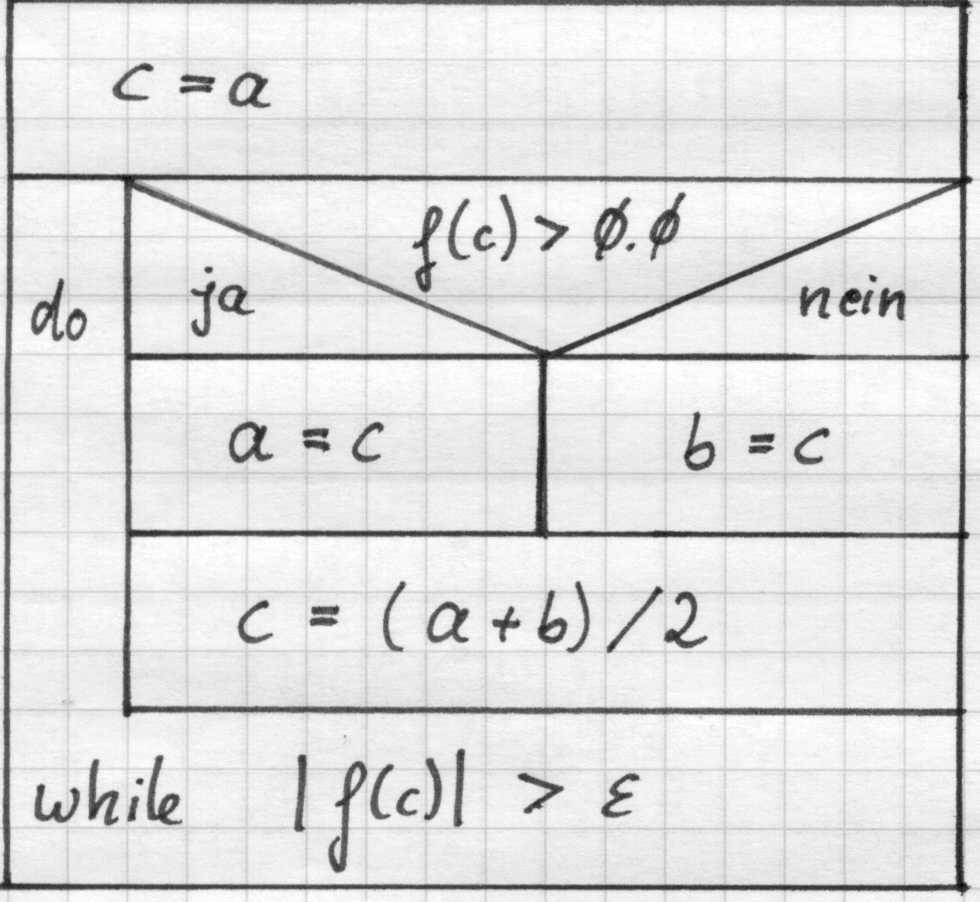
\includegraphics[scale=0.15]{GIF/p41a.eps}
% 
% 
% Obige Bisektion kann auch mittels eines
% abweisenden Zyklus realisiert werden.\index{Bisektion}
% \\
% % \begin{latexonly}
% %   \special{psfile=GIF/p41b.eps.gz
% % 	   hscale=20 vscale=20
% % 	   voffset=-180
% % 	  }
% %   \vspace{7cm}
% % \end{latexonly}
% % \htmladdimg{p41b_4.jpg}{}
% 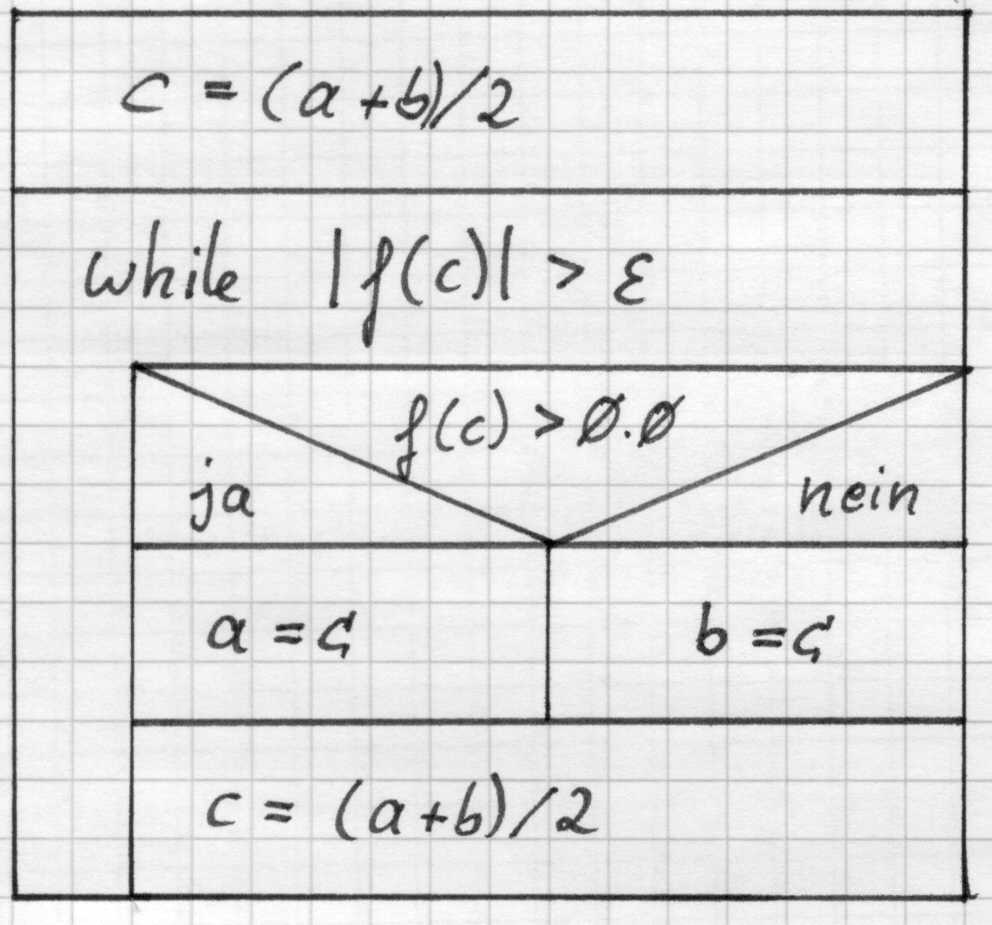
\includegraphics[scale=0.15]{GIF/p41b.eps}
%%%%%%%%%%%%%%%%%%%%%%%%%%%%%%%%%
\begin{minipage}{0.45\textwidth}
 \underline{nichtabweisender Zyklus}: \\
 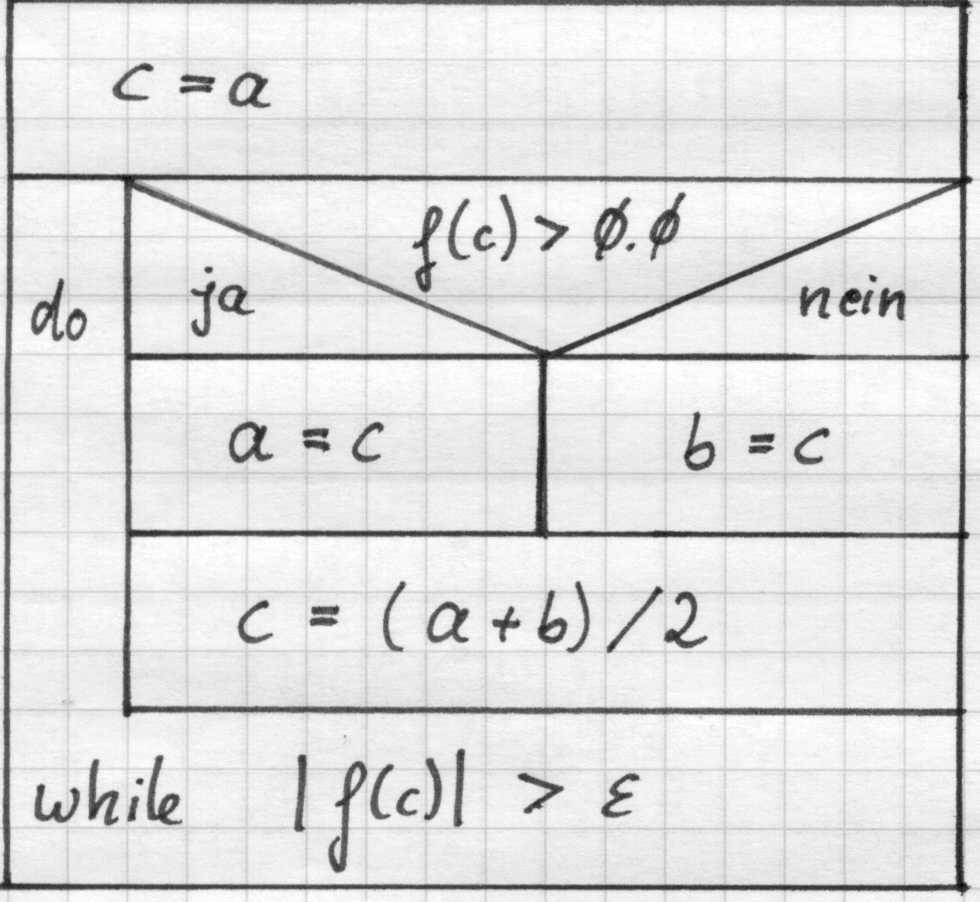
\includegraphics[scale=0.15]{GIF/p41a.eps}
\end{minipage}
\hfill
\begin{minipage}{0.45\textwidth}
 \underline{abweisender Zyklus}: \\
 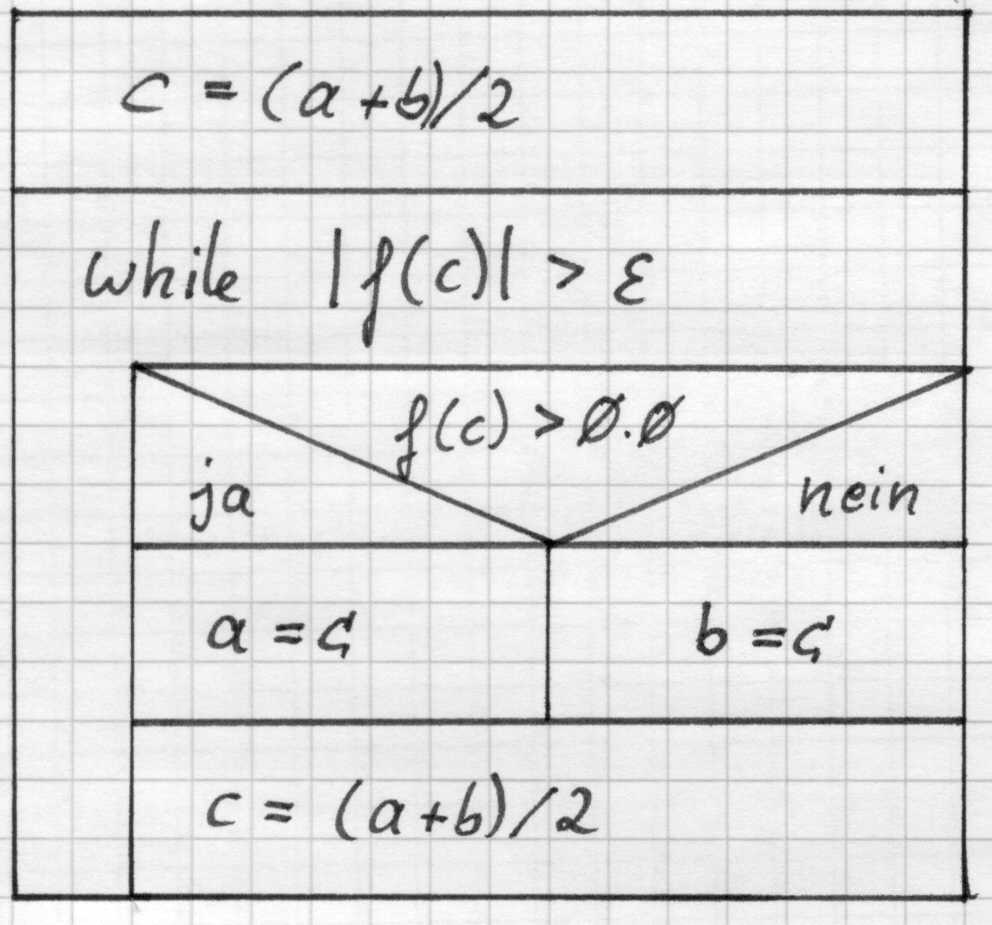
\includegraphics[scale=0.15]{GIF/p41b.eps}
\end{minipage}
\\
Wir realisieren obige Bisektion als nichtabweisenden Zyklus.\index{Bisektion}
%
\includecode[linerange={7-14,19-20,45-62,67-68}]{Ex462.cpp}{Bisektion als nichtabweisender Zyklus}
%

Da Gleitkommazahlen nur mit limitierter Genauigkeit\index{Gleitkommazahl!Genauigkeit}
arbeiten, resultiert
ein Abbruchtest $f(c) = 0$ meist in einem endlosen Programm.\index{Abbruchtest}
Dem ist ein Abbruchtest wie $|f(c)| < \varepsilon$ mit einer
vorgegebenen Genauigkeit $0< \varepsilon \ll 1$ vorzuziehen.

%\enlargethispage{1ex}
\underline{Bemerkung:}
Z"ahlzyklen (\verb|for|), welche \underline{mindestens einen} Zyklus
ausf"uhren, k"onnen sowohl durch abweisende (\verb|while|)
als auch durch nichtabweisende Zyklen (\verb|do while|)
"aquivalent ausgedr"uckt werden.
Diese "Aquivalenz kann bei Verwendung der Anweisungen in \S~\ref{p:4.8}
verloren gehen.
Falls in einem Z"ahlzyklus der Abbruchtest stets \texttt{false} ergibt, d.h.
der Schleifenk"orper wird nie ausgef"uhrt, dann ist
der entsprechende abweisende Zyklus nach wie vor "aquivalent. Jedoch
ist der nichtabweisende Zyklus nicht mehr "aquivalent, da der dortige
Schleifenk"orper auch in diesem Fall einmal abgearbeitet wird.
\bspfile{Loops.cpp}
%Siehe das Beispielfile~\textit{Loops.cpp}.
%
%
%
\section{Mehrwegauswahl (\texttt{switch}-Anweisung)}
\label{p:4.7}
%
Die Mehrwegauswahl erm"oglicht ein individuelles Reagieren
auf spezielle Werte einer Variablen.
\index{Mehrwegauswahl}\index{switch!Mehrwegauswahl}

\mbox{}\hfill
\begin{minipage}[t]{0.6\textwidth}
\begin{verbatim}
switch (<ausdruck>)
 {
   case <konst_ausdruck_1> :
        <anweisung_1>
	[break;]
   ...
   case <konst_ausdruck_n> :
        <anweisung_n>
	[break;]
   default:
        <anweisung_default>
 }
\end{verbatim}
\end{minipage}
\hfill\mbox{}

\textbf{Beispiel}: Ausgabe der Zahlw"orter f"ur die ganzzahlige Eingaben
	$\{1,2,3\}$.
	%dem Intervall~$[1,3]$.
%\includecode[linerange={7-14,19-20,45-62,67-68}]{Ex470.cpp}{Demonstration der Switch-Anweisung}
\includecode[firstline=5]{Ex470.cpp}{Demonstration der Switch-Anweisung}
%

Obige \verb|switch|-Anweisung k"onnte auch mit einer
Mehrfachverzweigung (Seite~\pageref{mehrweg}) implementiert werden,
jedoch werden in der \verb|switch|-Anweisung die einzelnen Zweige
explizit "uber die  \verb|break;|-Anweisung verlassen.
Ohne \verb| break; | wird zus"atzlich der zum nachfolgenden Zweig
geh"orige Block abgearbeitet.

Es ist in C++ \emph{nicht} m"oglich, \emph{Bereiche} anzugeben, etwa der Art
\texttt{case 7..11: Anweisung; break;} anstelle der korrekten
C++-Vorgangsweise~\cite[\S1.8.4]{Breymann:2017:DCP}
% \begin{verbatim}
\\[0.5ex]
\verb| case 7: case 8: case 9: case 10: case 11:| \\
\verb|    Anweisung;| \\
\verb|    break;|
% \end{verbatim}
%
%
%
\section[Unbedingte Steuerungs"ubergabe]{Anweisungen zur unbedingten Steuerungs"ubergabe}
\label{p:4.8}
%
%\begin{itemize}
\begin{description}
 \item[\texttt{break}] Es erfolgt der sofortige Abbruch
	 der n"achst"au{\ss}eren
	 \verb|switch|, \verb|while|, \verb|do-while|, \verb|for|
	 Anweisung.\index{break}
 \item[\texttt{continue}] Abbruch des aktuellen und Start des
 	n"achsten Zyklus einer \verb|while|, \verb|do-while|, \verb|for|
	Schleife.
	\bspfile{Ex480.cpp}
 \item[\texttt{goto <marke>}] Fortsetzung des Programmes an der mit
 	\\
	\verb|<marke> : <anweisung>|
	\\
	markierten Stelle.
\end{description}
%\end{itemize}

\underline{Bemerkung :} Bis auf \verb|break| in
der \verb|switch|-Anweisung sollten obige Anweisungen
sehr sparsam (besser gar nicht) verwendet werden, da
sie dem strukturierten Programmieren zuwiderlaufen und
im Extremfall einen gef"urchteteten Spaghetticode erzeugen.
Wenn man das strukturierte Programmieren gut beherrscht, dann kann die
gezielte Verwendung von \verb|break| und \verb|continue| zu schnellerem Code
f"uhren.

\textbf{Obige Anweisungen aus \S\ref{p:4.8} sind
im Rahmen dieser LV zur L"osung von "Ubungsaufgaben und im Test nicht erlaubt.}
Einzige Ausnahme ist \verb|break| in der \verb|switch|-Anweisung.
































\chapter{Ein Schnelleinstieg}
\label{p:1}
%
\section{Was ist ein Programm und was nützt es \emph{mir}?}
\label{p:1.1}
%
Eigentlich kennt jeder bereits Programme, jedoch versteht
man oft verschiedene Inhalte darunter.
\begin{itemize}
 \item Parteiprogramm	\hfill $\Longleftrightarrow$ \hfill Ideen
 \item Theaterprogramm	\hfill $\Longleftrightarrow$ \hfill Ablaufplanung
 \item Musikpartitur	\hfill $\Longleftrightarrow$ \hfill strikte Anweisungsfolge
 \item Windowsprogramm	\hfill $\Longleftrightarrow$ \hfill
 			interaktive Aktion mit dem Computer
\end{itemize}
\textbf{Programmieren} ist das Lösen von Aufgaben auf dem Computer
mittels eigener Software und beinhaltet alle vier Teilaspekte in obiger
Liste.

Eine typische Übungsaufgabe beinhaltet folgenden Satz:

\fbox {\begin{minipage} {0.95\textwidth}
 \mbox{}\hfill \vdots \hfill\mbox{} \\
 Ändern [editieren] Sie das Quellfile [source file] entsprechend
 der Aufgabenstellung, übersetzen [compilieren] und testen
 Sie das Programm.
\end{minipage}}
\\[1.5ex]

% \pagebreak[4]
\centerline {\Large Was (?) soll ich machen ?}
\mbox{}\\[1ex]
%
\begin{tabular}{p{0.25\textwidth}@{\qquad}p{0.5\textwidth}@{\qquad}p{0.15\textwidth}}
 Idee, z.B.\   math.\  Verfahren & Im Kopf oder auf dem Papier. \newline(Was soll der Computer machen?) & Programmidee \\
 $\hspace{0.09\textwidth}\Downarrow$  \\
%
 Idee f"ur den Computer aufbereiten &
 	Entwurf.\newline (Wie kann der Computer die Idee realisieren?) & Struktogramm \\
 $\hspace{0.09\textwidth}\Downarrow$  \\
%
 Idee in einer Pro\-grammier\-sprache formulieren.
  & Quelltext/Quellfile  editieren.\newline
   (Welche Ausdr"ucke darf ich verwenden?) & Programmcode \\
  $\hspace{0.09\textwidth}\Downarrow$  \\
%
 Quellfile f"ur den Computer "ubersetzen
  & File compilieren [und linken]. \newline("Ubersetzung in Prozessorsprache)
  & ausf"uhrbares Programm
  \\
 $\hspace{0.09\textwidth}\Downarrow$  \\
%
 Programmcode ausf"uhren
 & Programm mit verschiedenen Datens"atzen testen
 & Programmtest
\end{tabular}
\\[2ex]

\begin{samepage}
Bemerkungen:
\begin{enumerate}
 \item Software = ausf"uhrbares Programm + Programmcode  + \textbf{Ideen}
 \item Der Lernproze{\ss}  beim Programmieren erfolgt typischerweise von
 unten nach oben in der vorangegangenen "Ubersicht.
 \item Als Mathematiker sind vorrangig Ihre mathematischen Kenntnisse und Ideen gefragt,
   jedoch ist deren \textbf{eigenständig}e Umsetzung ein großer Vorteil bei vielen
   Arbeitsplätzen.
 \item Mit \textbf{fundierten Kenntnisse}n in einer Programmiersprache fällt es recht leicht 
 weitere Programmiersprachen zu erlernen.
\end{enumerate}
\end{samepage}

\fbox {\begin{minipage} {0.95\textwidth}
 \underline {\textbf {Warnung} :} Das Programm auf dem Computer wird
 \textbf{genau das} ausf"uhren, was im Programmcode beschrieben ist!
\end{minipage}}

Typischer Anf"angerkommentar:
%%\begin{minipage}[t] {0.55\textwidth}
 \textit{Aber das habe ich doch ganz anders gemeint.}
%%\end{minipage}

\fbox {\begin{minipage} {0.95\textwidth}
 \underline {\textbf {Merke} :} Computer sind strohdumm!
 Erst die (korrekte und zuverl"assige) Software nutzt die
 M"oglichkeiten der Hardware.
\end{minipage}}

\paragraph{Warum denn C++, es gibt doch die viel bessere Programmiersprache XYZ!}
Der Streit über die beste, oder die bessere Programmiersprache ist
so alt wie es Programmiersprachen gibt. Folgende Gründe sprechen gegenwärtig für C++:
\begin{itemize}
	\item C++ erlaubt sowohl \textbf{strukturiert}e, als auch \textbf{objektorientiert}e Programmierung.
	\item Strukturierte Programmierung ist die Basis jeder Programmierung im
	 wissenschaftlich-technischen Bereich.
	\item Sie können in C++ reine C-Programme schreiben wie auch rein objektorientiert programmieren,
	d.h., es ist eine sehr gute Trainingsplattform.
	\item C++ erlaubt ein höheres \textbf{Abstraktionsniveau} beim Programmieren, d.h.,
	 ich muß mich nicht um jedes (fehleranfällige) informatische Detail kümmern.
	 Andererseits kann ich genau dies tun, falls nötig.
	\item C++ ist eine Compilersprache, keine Interpretersprache, und damit können
	die resultierenden Programme schnell sein.
	\item Die \ghref{http://gcc.gnu.org/}{Gnu}-Compiler für C++ sind für
	  alle gängigen (und mehr) Betriebssysteme,
	 insbesondere Linux, Windows, Mac-OS, \textbf{kostenlos} verfügbar.
	 Desgleichen gibt es gute, kostenlose Programmierentwicklungsumgebungen (IDE)
	 wie \ghref{http://www.codeblocks.org/}{CodeBlocks} auf diesen. \\
	 Die \ghref{https://clang.llvm.org/}{clang}-Compiler sind ebenfalls sehr zu empfehlen.
	\item Seit ca.\  20 Jahren ist C++ meist unter den Top-5 im Programmiersprachenranking
	vertreten, siehe  verschiedene Rankings wie
	\ghref{http://www.tiobe.com/index.php/content/paperinfo/tpci/index.html}{TIOBE Index} oder
	\ghref{http://pypl.github.io/PYPL.html}{PYPL}.
    Die Programmiertechniken der anderen Spitzensprachen lassen sich mit C++ ebenfalls realisieren.
    \item C++ mit seinen Bibliotheken ist sehr gut dokumentiert, siehe
    \ghref{http://www.cplusplus.com}{cplusplus.com}, \ghref{http://en.cppreference.com/w/}{cppreference.com} und 
    natürlich \ghref{https://stackoverflow.com/}{stackoverflow} für schwierigen Fälle.
    \item C++ wird weiterentwickelt, der neue
    \ghref{http://en.wikipedia.org/wiki/C++11}{C++11, C++14, C++17} Standard ist in den
    Compilern umgesetzt und C++20 ist in Arbeit. 
    Wir werden die Möglichkeiten des Standards C++11 und C++-17 an passender Stelle benutzen.
\end{itemize}
%
%
%
%\pagebreak[4]
\newpage
\section{Das ``Hello World'' - Programm in C++}
\label{p:1.2}
%
Wir beginnen mit dem einfachen ``Hello World''-Programm, welches
nur den String ``Hello World'' in einem Terminalfenster ausgeben wird. Damit läßt sich
schon überprüfen, ob der Compiler und die IDE korrekt arbeiten
(und Sie diese bedienen können).
%
%\includecode[linerange={12-17,30-31}]{HelloWorld.cpp}{Quelltext von Hello World}
\includecode[firstline=12]{HelloWorld.cpp}{Quelltext von Hello World}
%
Der simple Code im Listing~\ref{lst:HelloWorld.cpp} enthält schon einige
grundlegende Notwendigkeiten eines C++-Programmes:
%
\begin{itemize}
  \item Kommentare bis zum Zeilenende werden mit \verb| // | eingeleitet.\index{Kommentar!C++}
  \\
  Der C-Kommentar \verb|/*    */| kann auch in C++ verwendet werden.\index{Kommentar!C}
  \item Jedes Programm benötigt eine Funktion \verb|main()|, genannt Hauptprogramm\index{main()}.
  \begin{itemize}
	  \item \verb|int main()|  deklariert (ankündigen) das Hauptprogramm in Zeile~4.
	  \item Die geschweiften Klammern \verb|{ }| in Zeilen~5 und~8 begrenzen den
	  Funktionskörper der Funktion \verb|main|.
	  \item In Zeile 7 wird der Ausdruck\index{Ausdruck} \verb| return 0 |
	  durch den Strichpunkt \verb| ; | zu einer Anweisung\index{Anweisung}
	  im Programm. Diese spezielle Anweisung beendet das Hauptprogramm
	  mit dem Rückgabewert 0.
  \end{itemize}
  \item Die Ausgabe in Zeile~6 benutzt die I/O-Bibliotheken von C++.
  \begin{itemize}
    \item \verb|cout | ist ein Bezeichner für die Ausgabe im Terminal.
    \item \verb|<< |  leitet den nachfolgenden String auf den Ausgabestrom (\verb|cout|) um.
      Dies kann wiederholt in einer Anweisung geschehen.
    \item \verb|endl |  ist der Bezeichner für eine neue Zeile im Ausgabestrom.
    \item Die Preprocessor-Anweisung (beginnt mit \verb|#|) in Zeile~1 inkludiert
      das, vom Compiler mitgelieferte, Headerfile\index{Headerfile} \emph{iostream}
      in den Quelltext. Erst dadurch können Bezeichner wie \verb|cout | und
       \verb|endl | der I/O-Bibliothek benutzt werden.
    \item Ohne Zeile~2 müssen der Ausgabestrom etc.\   über die explizite Angabe
    des Namensraumes \verb|std| angegeben werden, also als \verb| std::cout |.
    Mit Zeile~2 wird automatisch der Namensraum \verb|std| berücksichtigt wodurch
    auch \verb|cout|  identifiziert wird.
  \end{itemize}
\end{itemize}
%

\underline{Quelltext eingeben und compilieren, Programm ausf"uhren}:
\begin{enumerate}
 \item Quellfile editieren. \index{Quellfile!editieren} \\
       \texttt{LINUX> geany HelloWorld.cpp}
 \item Quellfile compilieren. \index{Quellfile!compilieren}\index{Compilieren!g++} \\
	\texttt{LINUX> g++ HelloWorld.cpp}
 \item Programm ausf"uhren. \index{Programm!ausf\"uhren} \\
	\texttt{LINUX> a.out} \qquad oder \\
	\texttt{LINUX> ./a.out} \qquad oder \\
	\texttt{WIN98> ./a.exe}
\end{enumerate}
%
%
\underline{Tip zum Programmieren}: \\
 Es gibt (fast) immer mehr als eine M"oglichkeit, eine Idee im
 Computerprogramm zu realisieren. \\
 $\Longrightarrow$ Finden Sie Ihren eigenen Programmierstil
 	und verbessern Sie ihn laufend.
%
%
%
\newpage
\section{Interne Details beim Programmieren}
\label{p:1.3}
%
Der leicht ge"anderte Aufruf zum Compilieren	\\
\texttt{LINUX> g++ -v HelloWorld.cpp}		\\
erzeugt eine längere Bildschirmausgabe, welche mehrere
Phasen des Compilierens anzeigt.
Im Folgenden einige Tips, wie man sich diese einzelnen Phasen
anschauen kann, um den Ablauf besser zu verstehen:
%
\begin{enumerate}
  \renewcommand {\labelenumi}{\alph{enumi})}
  \item \emph{Preprocessing}: \index{Preprocessing}
  	Headerfiles\index{Headerfile}
	(\textit{*.h}, \textit{*} und \textit{*.hpp}) werden zum
	Quellfile hinzugef"ugt (+ Makrodefinitionen, bedingte Compilierung) \\
	\texttt{LINUX> g++ -E HelloWorld.cpp > HelloWorld.ii} \\
	Der Zusatz \quad\texttt{> HelloWorld.ii}\quad lenkt die Bildschirmausgabe
	in das File \textit{HelloWorld.ii}. Diese Datei \textit{HelloWorld.ii}
	kann mit einem Editor angesehen werden und ist ein langes C++
	Quelltextfile.
  \item "Ubersetzen in \emph{Assemblercode}: \index{Assembler}
  	Hier wird ein Quelltextfile in der
	(prozessorspezifischen) Programmiersprache Assembler erzeugt. \\
	\texttt{LINUX> g++ -S HelloWorld.cpp} \\
	Das entstandene File \textit{HelloWorld.s} kann mit dem
	Editor angesehen werden.
 \item \emph{Objektcode} erzeugen: \index{Objektcode}
 	Nunmehr wird ein File erzeugt, welches die direkten Steuerbefehle,
	d.h. Zahlen f"ur den Prozessor beinhaltet. \\
	\texttt{LINUX> g++ -c HelloWorld.cpp} \\
	Das File \textit{HelloWorld.o} kann nicht mehr im normalen
	Texteditor angesehen werden sondern mit \\
	\texttt{LINUX> xxd HelloWorld.o}
 \item \emph{Linken}: \index{Linken}\index{Objektcode}\index{Bibliothek}
 	Verbinden aller Objektfiles und notwendigen Bibliotheken
	zum ausf"uhrbaren Programm \textit{a.out}\enspace. \\
	\texttt{LINUX> g++ HelloWorld.o}
\end{enumerate}
%
%
%
\section{Bezeichnungen in der Vorlesung}
\label{p:1.4}
%
\begin{itemize}
 \item Kommandos in einer Befehlszeile unter LINUX:\index{Compilieren!g++}\\
 	\texttt{LINUX> g++ [-o myprog] file\_name.cpp} \\
	Die eckigen Klammern \verb| [  ] | markieren optionale
	Teile in Kommandos, Befehlen oder Definitionen.
	Jeder Filename besteht aus dem frei w"ahlbaren Basisnamen
	(\textit{file\_name}) und dem Suffix (\textit{.cpp}) welcher
	den Filetyp kennzeichnet.
 \item Einige Filetypen nach dem Suffix: \index{Suffix}

  \nopagebreak
  \begin{tabular}{l@{\qquad}p{0.6\textwidth}}
  	Suffix 		& Filetyp \\ \hline
	%\textit{.c}	& C-Quelltextfile \index{Quellfile}\\
	%\textit{.h}	& C-Headerfile (auch C++), Quellfile mit vordefinierten
				%Programmbausteinen \index{Headerfile}\\
	\textit{.cpp}
			& C++ -Quelltextfile\\
	\textit{.h} %,\textit{.hpp} [\textit{.hh}]
			& C++ -Headerfile\\
	\textit{.o}	& Objektfile \index{Objektfile}\\
	\textit{.a}	& Bibliotheksfile (Library) \index{Bibliothek} \\
        \textit{.exe}	& ausf"uhrbares Programm (unter Windows)
  \end{tabular}
  \item Ein Angabe wie \qquad
  	$\cdots$ \verb| < typ > | $\cdots$
	\qquad bedeutet, da{\ss}  dieser Platzhalter durch
	einen Ausdruck des entsprechenden Typs ersetzt werden mu\ss.
\end{itemize}
%
%
%
\newpage
\section{Integrierte Entwicklungsumgebungen}
\label{p:1.5}
%
Obwohl nicht unbedingt daf"ur n"otig, werden in der Programmierung h"aufig IDEs
(Integrated Development Environments) benutzt, welche Editor, Compiler, Linker und
Debugger - oft auch weitere Tools enthalten.
In der LV benutzen wir freie \ghref{http://gcc.gnu.org/}{Compiler} und
\ghref{http://www.gnu.org/}{-entwicklungstools},
insbesondere die Compiler basieren auf dem GNU-Projekt und funktionieren
unabhängig von Betriebssystem und Prozessortyp. Damit ist der von Ihnen geschriebene Code
portabel und läuft auch auf einem Supercomputer
(allerdings nutzt er diesen nicht wirklich aus, dazu sind weitere LVs n"otig).
Grundlage des Kurses sind die g++-Compiler ab Version 4.7.1, da diese auch den neuen C++11-Standard unterstützen.
Gegebenenfalls muß der Code mit der zusätzlichen Option \verb| -std=c++11 | übersetzt werden.

Wir werden unter Windows die IDE \ghref{http://www.codeblocks.org/}{\textbf{Code::Blocks}}
Version 16.01 [Stand: Feb.~2016]
benutzen welche auf den GNU-Compileren und -Werkzeugen basiert.
Dies erlaubt die Programmierung unter Windows ohne die Portabilit"at zu verlieren, da diese IDE
auch unter LINUX verf"ugbar ist.
Sie k"onnen diese Software auch einfach privat installieren,
siehe \ghref{http://www.codeblocks.org/downloads/26\#windows}{Download}
(nehmen Sie \texttt{codeblocks-16.01mingw-setup.exe}) und das
\ghref{http://www.codeblocks.org/user-manual}{Manual}.
Installieren Sie in jedem Fall \textbf{vorher} das Softwaredokumentationstool
\ghref{http://www.doxygen.org}{doxygen} (und \ghref{http://cppcheck.sourceforge.net/}{cppcheck}),
da es nur dann automatisch in die IDE eingebunden wird.

Da die Entwicklungsumgebung alles vereinfachen soll, ist vor dem ersten Hello-World-Programm
etwas mehr Arbeit zu investieren.
\begin{enumerate}
 \item \texttt{Code::Blocks} aufrufen: \\
   auf dem \textbf{Desktop} das Icon \textbf{Code::Blocks} anklicken.
 \item In \texttt{Code::Blocks} ein neues \emph{Projekt} anlegen: \\
   \textbf{File $\longrightarrow$ New $\longrightarrow$ Project}
   \begin{enumerate}
     \item Im sich "offnenden Fenster das Icon  \textbf{Console Application} anklicken und
        dann auf \textbf{Go} klicken.
     \item Bei der Auswahl der Programmiersprache \textbf{C++} anklicken und dann \textbf{Next}.
     \item Den \textbf{Projektitel} angeben - hier bitte das Namensschema \emph{bsp\_nr} mit
          \emph{nr} als Nummer der abzugebenden "Ubungsaufgabe einhalten. \\
          Den \textbf{Folder} (das Verzeichnis) ausw"ahlen in welchem das Projekt gespeichert
          werden soll. Darin wird dann automatisch ein Unterverzeichnis mit dem Projektnamen angelegt.
          \\  \textbf{Next} klicken.
     \item Die \emph{Debug} und die \emph{Release configuration} aktivieren.
     %Bei den \textbf{Compiler} und \textbf{configuration} angeben und darauf achten, da"s
           %das Projekt als \textbf{C++-Projekt} markiert ist.
           Auf \textbf{Finish} klicken.
     \item Im Workspace erscheint das neue Projekt \emph{bsp\_1} welches in seinen
          \emph{Sources} das File \emph{main.cpp} enth"alt.
           Auf dieses File klicken.
     \item Im Editor sehen Sie nun folgenden Programmtext: \\
\begin{minipage}{0.5\textwidth}
%
{\scriptsize
\begin{boxedverbatim}
#include <iostream>

using namespace std;

int main()
{
    cout << "Hello world!" << endl;
    return 0;
}
\end{boxedverbatim}
}
%
\end{minipage}
  \item Compilieren und Linken: \textbf{Build $\longrightarrow$ Build}
  \item Programm ausführen: \textbf{Build $\longrightarrow$ Run}
  \item Speichern dieser Datei: \textbf{File $\longrightarrow$ Save}
   \end{enumerate}
\end{enumerate}

\newpage
\section{Erste Schritte mit Variablen}
\label{p:1.6}
%
Wir beginnen mit dem einfachen ``Hello World''-Programm, welches
nur den String ``Hello World'' in einem Terminalfenster ausgibt.
Damit läßt sich schon überprüfen, ob der Compiler und die IDE korrekt arbeiten
(und Sie dies bedienen können).
Anschließend arbeiten wir mit ein paar einfachen Variablen.
%
%\includecode[linerange={12-17,30-31}]{HelloWorld_2.cpp}{Erweitertes ``Hello World''}
\includecode[firstline=2]{HelloWorld_2.cpp}{Erweitertes ``Hello World''}
%
Obiger Code enthält bekannte Teile aus dem Listing~\ref{lst:HelloWorld.cpp}, wir werden
kurz die neuen Zeilen erläutern:
\begin{itemize}
	\item[{[2]}] Die Deklarationen für den Datentyp (die Klasse) \texttt{std::string}
	  werden inkludiert. In Zeile~3 wird der Namensraum für \verb|std| freigegeben.
	\item[{[8]}] Ein \ghref{http://de.wikipedia.org/wiki/Integer_(Datentyp)\#Maximaler_Wertebereich_von_Integer}
	{ganzzahlige Variable}~\texttt{i} wird deklariert und darf damit in
	  den nachfolgenden Zeilen des Gültigkeitsbereichs zwischen \verb| { |
	  und  \verb| } | verwendet werden, also bis zur Zeile~22. Die Variable~\texttt{i}
	  kann ganzzahlige Werte aus $[-2^{-31},2^{-31}-1]$ annehmen.
    \item[{[10]}] Die Variable~\texttt{i} wird über den Terminal (Tastatureingabe)
     eingelesen. \verb| cin | und \verb| >> | sind Eingabestrom und -operator analog
     zur Ausgabe mit \verb| cout | und \verb| << |.
    \item[{[12]}] Die Variable~\texttt{i} wird gemeinsam mit einem beschreibenden String
     (Zeichenkette) ausgegeben.
    \item[{[14]}] Deklaration der Gleikommazahlen einfacher Genauigkeit
     (engl.: \ghref{http://de.wikipedia.org/wiki/IEEE_754\#Zahlenformate_und_andere_Festlegungen_des_IEEE-754-Standards}{single precision})
    \texttt{a} und \texttt{b}.
    \item[{[16]}] Einlesen von Werten für \texttt{a} und \texttt{b}. Ausgabe der
     Variablenwerte in Zeile~17.
    \item[{[19]}] Deklaration der Gleikommavariablen~\texttt{c}  und gleichzeitige Definition
    (Zuweisen eines Wertes) aus den Variablen \texttt{a} und \texttt{b}.
      Hierbei ist \verb| = | der Zuweisungsoperator und \verb| + | der Additionsoperator
      für Gleitkommazahlen.\index{Operator!Zuweisungs-}\index{Operator!Additions-}
    \item[{[20]}] Deklaration und gleichzeitige Definition eines konstanten (\texttt{const}) Strings~\texttt{ss}. Das Schlüsselwort legt fest, daß der \texttt{ss} zugewiesene Wert nicht mehr
      verändert werden kann.
    \item[{[21]}] Gemeinsame Ausgabe des konstanten Strings und der Gleikommavariablen.
    \item Mit \verb|{ }|  eingeschlossene Bereiche eines Quelltextes
	  definieren die Grenzen eines Gültigkeitsbereiches (scope)\index{Block}\index{scope}
	  von darin definierten Variablen.
\end{itemize}

Damit haben wir eine Grundlage, um uns in die Programmierung mit C++
schrittweise einzuarbeiten.

\chapter{Variablen und Datentypen}
\label{p:2}
%
\section{Variablen}
\label{p:2.1}
Jedes sinnvolle Programm bearbeitet Daten in irgendeiner Form.
Die Speicherung dieser Daten erfolgt in Variablen.\index{Variable|(}

Allgemeine Form der Variablenvereinbarung: \\
\centerline {\texttt {
  <typ> <bezeichner1> [, bezeichner2] ;
}}

\noindent
Die Variable
\begin{minipage}[t] {0.8\textwidth}
 \begin{enumerate}
   \renewcommand {\labelenumi}{\roman{enumi})}
   \item ist eine symbolische Repr"asentation (Bezeichner/Name) f"ur
   	den Speicherplatz von Daten.
   \item  wird beschrieben durch Typ und
   	Speicherklasse.\index{Variable!Typ}\index{Variable!Speicherklasse}.
   	Der Datentyp \texttt{<typ>} einer Variablen bestimmt die zulässigen Werte
   dieser Variablen.
   \item Die Inhalte der Variablen, d.h., die im Speicherplatz befindlichen
   	Daten, "andern sich w"ahrend des Programmablaufes.
 \end{enumerate}
\end{minipage}

%
\subsection{Einfache Datentypen}
\label{p:2.2}
%
Daten im Computer basieren auf dem binären Zahlensystem von
Gottfried Wilhelm Leibniz\footnote{Gottfried Wilhelm Leibniz,
\textborn 1.7.1646 in Leipzig, \textdied 14.11.1716 in Hannover}
worin alle ganzen Zahlen durch die Summation von
mit~0 oder~1 gewichteten Zweierpotenzen dargestellt werden können. So wird die Zahl
117 im Dezimalsystem durch
$$ 117_{(10)} =
01110101_{(2)} = 0 \cdot 2^{7} + 1 \cdot 2^{6} + 1 \cdot 2^{5} +
 1 \cdot 2^{4} + 0 \cdot 2^{3} + 1 \cdot 2^{2} + 0 \cdot 2^{1} + 1 \cdot 2^{0}$$
binär dargestellt.
Die grundlegende Informationseinheit im Computer ist das \emph{Bit} welches
genau einen der zwei Zustände~1 oder~0 annehmen kann
(ja/nein, true/false). Somit werden in obiger Binärendarstellung von 117
genau 8~Bit benötigt. Diese 8~Bit stellen die kleinste Grundeinheit des
Datenzugriffs bei heutigen Computern dar und werden als ein \emph{Byte} bezeichnet.
\index{bit}\index{Byte}

%
Aufbauend auf der Speichereinheit Byte sind die in Tabelle~\ref{tab:2.1.1}
dargestellten, \ghref{https://en.cppreference.com/w/cpp/language/types}{grundlegenden Datentypen} in C++ vorhanden.
%
\begin{table}[htb]
	\label{tab:2.1.1}
\mbox{}\hfill
\begin{tabular}{l@{\quad}c@{\quad}l@{\quad}p{0.3\textwidth}}
    \hline\hline
 Typ		& \hspace{-6ex}Speicherbedarf& Inhalt	& mögliche Werte \\
 		& \hspace{-6ex}in Byte	&		&	\\  \hline\hline
 \texttt{byte}	& 1		& Byte & $0x00000000 \ldots 0x11111111$
	\\ \hline 
 \texttt{char}	& 1		& ASCII-Zeichen & 'H', 'e', '$\backslash$n'
	\\
 \texttt{wchar\_t}	& 2$|$4 & Unicode (Win$|$Unix) & Ä. ß, $\gamma$, $\Omega$, $\daleth$, $\aleph$
	\\    
     \hline
 \texttt{bool}	& 1		& Booleanvariable & \verb|false|, \verb|true|\quad [erst ab C90]
	\\ \hline
%
 \texttt{signed char} & 1		&	&  $[-128, 127]$ ; -117, 67 \\
 \texttt{unsigned char} & 1		&	&    $[0, 255]$ ;  139, 67\\
 \texttt{short} [\texttt{int}] 	& 2		& 	& $[-2^{15},2^{15}-1]$ ; -32767 \\
 \texttt{unsigned short} [\texttt{int}] & 2		& 	& $[0,2^{16}-1]$ ;  40000\\
 \texttt{int}	& 4		&	Ganze Zahlen	&  $[-2^{31},2^{31}-1]$ \\
 \texttt{unsigned} [\texttt{int}]	& 4		&	(integer)	&  $[0,2^{32}-1]$ \\
 \texttt{long}  [\texttt{int}]  	& 4		&	& wie \texttt{int} \\
 \texttt{unsigned long}  [\texttt{int}] 	& 4		&		& wie \texttt{unsigned int} \\
 \texttt{long long}  [\texttt{int}]  		& 8		&		&  $[-2^{63},2^{63}-1]$  \\
 \texttt{unsigned long long}  [\texttt{int}]& 8		&		& $[0,2^{64}-1]$ \\
 \texttt{size\_t}  & 		&	implementierungsabhängig	&  \texttt{unsigned long long int}
 \\ \hline
%
 \texttt{float} & 4		& Gleitkommazahlen& 1.1, -1.56e-32 \\
 \texttt{double}& 8		& (floating point numbers)		& 1.1, -1.56e-132, 5.68e+287
 	\\ \hline\hline
\end{tabular}
\hfill\mbox{}
	\caption{Speicherbedarf grundlegender Datentypen [Stand 03/2019]}
\end{table}
\index{char}\index{bool}\index{int}\index{float}\index{double}
%
\begin{itemize}
 \item Standardcharacterdaten speichern in einem Byte (=~8~bit) genau ein
  \ghref{http://de.wikipedia.org/wiki/Ascii\#ASCII-Tabelle}{ASCII}- oder Sonderzeichen, d.h.,
  die kodierten Buchstaben, Ziffern und Sonderzeichen werden durch eine ganze Zahl aus $[0,255=2^{8}-1]$
  (\texttt{unsigned char}) dargestellt. 
 \item Der Speicherbedarf von ganzzahligen Datentypen (\texttt{short int}, \texttt{int},
 \texttt{long int}, \texttt{long long int} )\index{Integer}
 	kann von Compiler und Betriebssystem (16/32/64 bit) abh"angen.
	Es empfiehlt sich daher, die einschl"agigen Compilerhinweise zu lesen
	bzw.\  mit dem \texttt{sizeof}-Operator mittels
	\texttt{sizeof(<typ>)} oder \texttt{sizeof(<variable>)}\index{sizeof()}
	die tats"achliche Anzahl der ben"otigten Bytes zu ermitteln.
	Siehe dazu auch das Listing~\ref{lst:DataTypes.cpp}.
 \item Wir werden meist den Grundtyp \texttt{int} f"ur
 	den entsprechenden Teilbereich der ganze Zahlen und
 	\texttt{unsigned int} f"ur nat"urliche Zahlen verwenden.
	Die Kennzeichnung \texttt{unsigned} sowie das ungebräuchliche \texttt{signed} kann auch in
	Verbindung mit anderen Integertypen verwendet werden.
    Falls der gewählte Datentyp stets genau 16 bit beinhalten soll, dann können 
    \ghref{https://en.cppreference.com/w/cpp/types/integer}{Fixed Integer Types} wie \verb|int16_t| benutzt werden.
 \item Floating point numbers sind im Standard \ghref{https://de.wikipedia.org/wiki/IEEE_754}{IEEE 754} definiert.
 Die Anzahl der Mantissenbits (\texttt{float}: 23; \texttt{double}: 52) bestimmt deren relative Genauigkeit,
  d.h., das Maschinen-$\varepsilon$, welches die kleinste Zahl des Datentyps darstellt
  für die $1+\varepsilon > 1$ noch gilt
  (\texttt{float}: $2^{-(23+1)}$; \texttt{double}: $2^{-(52+1)}$).
  Siehe dazu auch das \ghref{https://de.wikipedia.org/wiki/Gleitkommazahl\#Hidden_bit}{hidden bit}.
\end{itemize}
\includecode[linerange={4-8,15-15,65-66,75-76}]{DataTypes.cpp}{Abfrage der Speichergröße von Datentypen}
%
%
%
\subsection{Bezeichner von Variablen}
\label{p:2.1.2}
%
Die Variablenbezeichner müssen gewissen Regeln folgen (\ghref{http://de.wikipedia.org/wiki/C_(Programmiersprache)\#Deklarationen}{wiki}):
\begin{itemize}
	\item Das erste Zeichen eines Bezeichners einer Variablen muss ein Buchstabe oder Unterstrich sein.
	\item Die folgenden Zeichen dürfen nur die Buchstaben A–Z und a–z, Ziffern und der Unterstrich sein.
	\item Ein Bezeichner darf kein Schlüsselwort der Sprache – zum Beispiel if, void und auto – sein.
 \item C/C++ unterscheidet zwischen Gro\ss - und Kleinschreibung, d.h.,
 	\texttt{ToteHosen} und \texttt{toteHosen} sind unterschiedliche
	Bezeichner!
	\bspfile{Ex210.cpp}
 %\item Laut originalem C-Standard sind die ersten 8 Zeichen eines
 	%Variablenbezeichners
 	%signifikant, d.h., \texttt{a2345678A} und \texttt{a2345678B}
	%w"urden nicht mehr als verschiedene Bezeichner wahrgenommen.
	%Mittlerweile sehen Compiler mehr Zeichen als signifikant an
	%(C9X Standard: 63 Zeichen).
\end{itemize}
%
\begin{table}[hbt]
	\label{tab:2.1.2}
\mbox{}\hfill
\begin{tabular}{l@{$\;\;$}||@{$\;\;$}r@{\qquad\qquad}p{0.3\textwidth}}
  G"ultig & Ung"ultig & Grund \\ \hline
  \texttt{i} \\
  \texttt{j} \\
  \texttt{ijl} \\
  \texttt{i3}	& \texttt{3i}	& 3 ist kein Buchstabe \\
  \texttt{\_3a}	& \texttt{\_3*a} & * ist Operatorzeichen \\
  \texttt{Drei\_mal\_a} & \texttt{b-a} & - ist Operatorzeichen \\
  \texttt{auto1} & \texttt{auto} & \texttt{auto} ist Schl"usselwort
\end{tabular}
\hfill\mbox{}
\caption{Einge erlaubte und nicht erlaubte Variablenbezeichner}
\end{table}
%
\index{Variable|)}
%
%
%
\subsection{G"ultigkeit von Bezeichnern}
\label{p:2.1.3}
%
Die Bezeichner von Variablen, Konstanten etc. sind im Regelfall
lokal, d.h., ein Bezeichner ist nur innerhalb seines, von \verb|{ }|
begrenzten Blockes von Codezeilen gültig, in welchem dieser Bezeichner
deklariert wurde. Daher nennt man diesen Block den
Gültigkeitsbereich (scope)\index{Block}\index{scope}
dieser Variablen.
Siehe dazu Listing~\ref{lst:HelloWorld.cpp} und ~\S\ref{p:4.2}.
%
%
\subsection{Konstante mit Variablennamen}
\label{p:2.2.6}
%
\index{Konstante|(}%
Wird eine Variablenvereinbarung zus"atzlich mit dem
Schl"usselwort \texttt{const} gekennzeichnet, so kann diese
Variable nur im Vereinbarungsteil initialisiert werden und danach nie
wieder, d.h., sie wirkt als eine Konstante.
\includecode[firstline=6]{Ex226.cpp}{Definition und Deklaration von Konstanten und Variablen}
%
Nach der Deklaration in Zeile~6 ist die Variable~\texttt{i} noch nicht mit einem Wert belegt,
d.h., sie hat einen undefinierten Status.
In Zeile~7 würde der Wert von~\texttt{i} zufällig sein, je nachdem was gerade
in den reservierten 4~Byte als Bitmuster im Computerspeicher steht.
Damit wäre das Ergebnis einer Berechung mit~\texttt{i} nicht vorhersagbar
(nicht deterministisch) und damit wertlos.

Also sollte~\texttt{i} gleich bei der Deklaration auch definiert (initialisiert) werden.
In C++ kann man ausnutzen, daß Deklarationsteil und Implementierungsteil gemischt werden können.
Dies wird im Listing~\ref{lst:Ex226_b.cpp} ausgenutzt, sodaß die Variable~\texttt{i}
erst in Zeile~4 deklariert wird, wo dieser auch gleich ein sinnvoller
Wert zugewiesen werden kann.
%
\includecode[linerange={11-13,15-16}]{Ex226_b.cpp}{Variablen erst bei Gebrauch deklarieren}
\index{Konstante|)}
%
%
\section{Literale Konstanten}
\label{p:2.22}
%
Die meisten Programme, auch \textit{HelloWorld.cpp}, verwenden
im Programmverlauf unver"anderliche Werte, sogenannte Literale und Konstanten.
\index{Literale|(}
Literale Konstanten sind Werte ohne Variablenbezug welche in Ausdrücken explizit angegeben werden und zusätzliche
Typinformationen enthalten können.
%Konstanten sind namentlich gekennzeichnete Daten deren Werte nach der Deklaration und ihrer gleichzeitigen
%Definition/Initialisierung nicht mehr verändert werden.
%
\subsection{Integerliterale}
\label{p:2.22.1}
%
Dezimalliterale (Basis 10): \hfill
\begin{minipage}[t] {0.5\textwidth}
\begin{verbatim}
   100        // int;     100
   512L       // long;    512
   128053     // long; 128053
\end{verbatim}
\end{minipage}

Oktalliterale (Basis 8): \hfill
\begin{minipage}[t] {0.5\textwidth}
\begin{verbatim}
   020        // int;      16
   01000L     // long;    512
   0177       // int;     127
\end{verbatim}
\end{minipage}

Hexadezimalliterale (Basis 16): \hfill
\begin{minipage}[t] {0.5\textwidth}
\begin{verbatim}
   0x15       // int;      21
   0x200      // int;     512
   0x1ffffl   // long; 131071
\end{verbatim}
\end{minipage}\index{Literale!Integer}
%
%
\subsection{Gleitkommaliterale}
\label{p:2.22.2}
%
Gleitkommaliterale werden als \texttt{double} interpretiert solange
dies nicht anderweitig gekennzeichnet ist.
\index{Literale!Gleitkommazahl}\index{Gleitkommazahl}
\\
Einige Beispiele im folgenden:
\begin{minipage}[t] {0.6\textwidth}
\begin{verbatim}
   17631.0e-78
   1E+10              //   double: 10000000000
   1.                 //   double: 1
   .78                //   double: 0.78
   0.78
   -.2e-3             //   double: -0.0002
   -3.25f             //   single: -3.25
\end{verbatim}
\end{minipage}
%
%
\subsection{Zeichenliterale (Characterliterale)}
\label{p:2.22.3}
%
Die Characterliterale beinhaltet das Zeichen zwischen den zwei Apostrophen
\texttt{'} :
\begin{minipage}[t] {0.9\textwidth}
\begin{verbatim}
   'a', 'A', '@', '1' //  ASCII-Zeichen
   ' '                //    Leerzeichen
   '_'                //    Unterstreichung/Underscore
   '\''               //    Prime-Zeichen '
   '\\'               //    Backslash-Zeichen  \
   '\n'               //  neue Zeile
   '\0'               //  Nullzeichen NUL
\end{verbatim}
\end{minipage}\index{Literale!Character}\index{Ausgabe!neue Zeile}
%
%
\subsection{Zeichenkettenkonstanten (Stringkonstanten)}
\label{p:2.22.4}
%
Die Zeichenkette beinhaltet die Zeichen zwischen den beiden
Anführungszeichen \texttt{"} :
\begin{minipage}[t] {0.8\textwidth}
\begin{verbatim}
   "Hello World\n"    //    \n is C-Stil fuer neue Zeile (C++: endl)
   ""                 //    leere Zeichenkette
   "A"                //    String "A"
\end{verbatim}
\end{minipage}\index{Konstante!String}

Jede Zeichenkette wird automatisch mit dem
(Character-) Zeichen \verb|'\0'| abgeschlossen
(\textit{``Hey, hier h"ort der String auf!''}).
Daher ist \verb|'A'| ungleich \verb|"A"|, welches
sich aus den Zeichen  \verb|'A'| und \verb|'\0'|
zusammensetzt und somit 2~Byte zur Speicherung ben"otigt.
\includecode[firstline=4]{Ex224.cpp}{Länge von String und Character}
%
\index{Literale|)}
%
%
\section{Einige h"ohere Datentypen in C++}
\label{p:2.3}
%
Die Standardbibliothek und
die \textbf{S}tandard \textbf{T}emplate \textbf{L}ibrary (STL) stellen eine gro"se Auswahl
an komfortablen h"oheren Datenkonstrukten (genauer: \emph{Klassen} und \emph{Container}) zur Verf"ugung, welche
das Programmieren vereinfachen.
Die intensive Anwendung der Container f"ur eigene Datenstrukturen (und \emph{Klassen})
erfordert Kenntnisse in Klassenprogrammierung, Vererbung und  Templates, welche wir erst später behandeln werden.
Um aber schon mit diesen höheren Datentypen arbeiten zu können,  erfolgt hier ein kurze Einführung
in \texttt{string}, \texttt{complex},
\texttt{vector} und \texttt{valarray}.
Vertiefend und weiterf"uhrend seien dazu u.a.
\cite{KirchPrinz:2002:OOP, KuhlinsSchader:2002:DCS, SatirBrown:1995:PCP}
empfohlen.
%

\subsection{Die Klasse string}
\label{p:2.3.1}
Diese Standardklasse \texttt{string}~\cite[\S~18]{KirchPrinz:2002:OOP}
erlaubt eine komfortable Zeichenkettenverarbeitung
\includecode[firstline=4]{demoString.cpp}{Erste Schritte mit \texttt{string}}
%
Die Konvertierung von Zahlen in Strings und umgekehrt wird \ghref{http://www.cplusplus.com/articles/D9j2Nwbp/}{hier} erläutert und ist noch komfortabler mit
  \texttt{to\_string} und \texttt{stof}.
%
%\newpage

\subsection{Die Klasse complex}
\label{p:2.3.2}
Die Standardklasse \texttt{complex<T>}~\cite[p.~677]{KirchPrinz:2002:OOP}
erlaubt die Verwendung komplexer Zahlen \bspfile{demoComplex.cpp} in der gewohnten Weise.
Bei der Variablendeklaration mu"s der Datentyp der Komponenten der komplexen Zahl in
Dreiecksklammern angegeben werden. Hier machen eigentlich nur \verb|<double>| oder
\verb|<float>| einen Sinn.
%
\includecode[firstline=2]{demoComplex.cpp}{Erste Schritte mit \texttt{complex}}
%

\subsection{Die Klasse vector}
\label{p:2.3.4}
Die Containerklasse \texttt{vector<T>}~\cite[\S~5.1]{KuhlinsSchader:2002:DCS}
erlaubt die Verwendung von Vektoren \bspfile{demoVector.cpp} in vielf"altiger Weise, insbesondere
bei dynamisch ver"anderlichen Vektoren.
Bei der Variablendeklaration mu"s der Datentyp der Komponenten in
Dreiecksklammern angegeben werden. Wir werden meist \verb|<double>|,
\verb|<float>| oder \verb|<int>| verwenden, obwohl alle (korrekt implementierten) Klassen
hierf"ur benutzt werden d"urfen.
Die Klasse  \texttt{vector<T>} enh"alt keine Vektorarithmetik.
%
\subsubsection{Statischer Vektor}
Nachfolgender Code demonstriert den Einsatz eines statischen Vektors, d.h.,
die Anzahl der Vektorelemente is a~priori bekannt.
Mit \texttt{resize(\emph{laenge})} kann diese Anzahl der Elemente auf einen neuen Wert
ge"andert werden (dies ist eigentlich schon dynamisch). Die neuen Elemente m"ussen danach noch
mit Werten initialisiert werden.
%
\includecode[firstline=4]{demoVector.cpp}{Erste Schritte mit \texttt{vector} als statischem Vektor}
%

\subsubsection{Dynamischer Vektor}
Obiger Code behandelt Vektoren konstanter L"ange. Wenn die Anzahl der Vektorelemente a~priori unbekannt ist,
dann kann ein vorhandener Vektor durch Benutzung der Methode \texttt{push\_back(\emph{value})} um ein
weiteres Element mit dem Wert~\emph{value} verl"angert werden.
%
\includecode[firstline=2]{demoVector_dynamisch.cpp}{Erste Schritte mit \texttt{vector} als dynamischem Vektor}
%

\subsubsection{Ausgabe eines Vektor}
Leider k"onnen die Vektoren aus den vorherigen Beispielen nicht einfach mittels
\verb|cout << bb| ausgegeben werden. Ein solcher Versuch f"uhrt zu sehr kryptischen Fehlermeldungen
des Compilers. Es gibt drei prinzipielle M"oglichkeiten zur Ausgabe der Elemente eines
Vektor \verb|vector<int> bb|~:
\begin{enumerate}
  \item durch Ausgabe in einem \textrm{for}-Loop (konventionell),
  \item durch Kopieren auf den Ausgabestream (benutzt Algorithmus \texttt{copy} aus der STL),
  \item durch Definition einer Funktion f"ur den Ausgabeoperator \verb|<<| (Operator"uberladung).
\end{enumerate}
Alle 3 M"oglichkeiten werden in nachfolgendem Code demonstriert wobei jeweils exakt dieselbe Ausgabe
erzielt wird. Der Sprung auf die n"achste Ausgabezeile (\verb|cout << endl| nach jeder Variante)
wurde weggelassen.%\exfile{Ex234\_b.cpp}
Die Methoden \verb|begin()| und \verb|end()| zeigen auf das erste Elemente und das
hinterletzte Element (Diese beiden Methoden liefern Iteratoren zur"uck).
\includecode[firstline=2]{Ex234_b.cpp}{Ausgabe eines \texttt{vector}}
%

\subsection{\mbox{}$^{*}$Die Klasse valarray}
\label{p:2.3.3}
Die (nicht Standard) Klasse \texttt{valarray<T>}~\cite[p.~687]{KirchPrinz:2002:OOP}
erlaubt die Verwendung numerischer Vektoren \bspfile{demoValarray.cpp} wie sie von
\textsc{MatLab} bekannt sind. Insbesondere sind Vektorarithmetik und mathematische Funktionen vorhanden.
Bei der Variablendeklaration mu"s der Datentyp der Komponenten in
Dreiecksklammern angegeben werden. Wir werden \verb|<double>|,
\verb|<float>| oder \verb|<int>| verwenden.
%
\includecode[firstline=2]{demoValarray.cpp}{Vektorarithmetik mit \texttt{valarray}}
%
%Die Template-Klasse \texttt{valarray<T>} ist nicht in allen STL-Distributionen vorhanden.



























\chapter[Operatoren]{Ausdr"ucke, Operatoren und mathematische Funktionen}
\label{p:3}
%
\begin{itemize}
 \item \textbf{Ausdr"ucke} bestehen aus Operanden und Operatoren.\index{Ausdruck}
 \item \textbf{} sind Variablen, Konstanten oder wieder Ausdr"ucke.\index{Operanden}
 \item \textbf{Operatoren} f"uhren Aktionen mit Operanden aus.\index{Operator}
\end{itemize}
%
%
\section{Zuweisungsoperator}
\label{p:3.1}
%
Der Zuweisungsoperator
\verb| <operand_A> = <operand_B>| weist dem linken Operanden, welcher eine
Variable sein mu"s, den Wert des rechten Operanden zu.

Zum Beispiel ist im Ergebnis der Anweisungsfolge
\includecode[linerange={10-10,12-15,30-30}]{Ex310.cpp}{Anweisungsfolge}
%
der Wert von \verb|x| gleich 0 und der Wert von \verb|y| gleich 4.
Hierbei sind \verb|x|, \verb|y|,  \verb|0|, \verb|x+4|
Operanden, wobei letzterer gleichzeitig ein Ausdruck, bestehend
aus den Operanden \verb|x|, \verb|4| und dem Operator \verb|+|, ist.
Sowohl \verb|x = 0| als auch \verb|y = x + 4| sind Ausdr"ucke.
Erst das abschlie{\ss}ende Semikolon \verb| ; | wandelt diese Ausdr"ucke
in auszuf"uhrende Anweisungen!

Es k"onnen auch Mehrfachzuweisungen auftreten.
Die folgenden drei Zuweisungsgruppen sind "aquivalent.
\includecode[linerange={10-11,20-22,30-30},label=Ex310_b.cpp]{Ex310.cpp}{Äquivalente Zuweisungen}
%
\section{Arithmetische Operatoren}
\label{p:3.2}
%
\subsection{Un"are Operatoren}
\label{p:3.2.1}
%
Bei un"aren Operatoren tritt nur ein Operand auf.

%
\begin{tabular} {l@{\quad}p{0.6\textwidth}@{\quad}l}
 Operator & Beschreibung & Beispiel \\ \hline
 \verb|-|	& Negation & \verb|-a|
\end{tabular}
%
%
\subsection{Bin"are Operatoren}
\label{p:3.2.2}
%
Bei bin"aren Operatoren treten zwei Operanden auf.
Der Ergebnistyp der Operation h"angt von den Operanden ab.
\index{Operator!arithmetischer}
%

\noindent
\begin{tabular} {l@{\quad}p{0.6\textwidth}@{\quad}l}
 Operator & Beschreibung & Beispiel \\ \hline
 \verb|+| & Addition & \verb|b + a| \\
 \verb|-| & Subtraktion & \verb|b - a| \\
 \verb|*| & Multiplikation & \verb|b * a| \\
 \verb|/| & Division (! bei Integer-Werten !)& \verb|b / a| \\
 \texttt{\%} & Rest bei ganzzahliger Division& \texttt{b \% a}
\end{tabular}

Die Division von Integerzahlen berechnet den ganzzahligen Anteil
der Division, d.h., \verb| 8 / 3 | liefert \verb| 2 | als Ergebnis.
Falls aber der Wert \verb| 2.666666 | herauskommen soll, mu{\ss}
mindestens einer der Operatoren in eine Gleitkommazahl umgewandelt werden,
wie im Listing~\ref{lst:Ex320.cpp} zu sehen ist.\index{Gleitkommazahl}
%
\includecode[linerange={10-20,61-61}]{Ex320.cpp}{Fallen und Typumwandlung (Casting) bei Integeroperationen}

\textbf{Achtung:} Der Modulo einer negativen Zahl wird in~C++ nicht so berechnet, wie man
es seitens der Algebra erwarten w"urde, z.B.,
\verb| -13 % 4 | liefert~\verb| -1 | statt~\verb| 3 |.

Bzgl. der Vorrangregeln f"ur Operatoren sei auf die Literatur verwiesen,
die alte Regel ``\textit{Punktrechnung geht vor Strichrechnung}'' gilt
auch in C/C++. Analog werden Ausdr"ucke in runden Klammern
\verb| ( <ausdruck> ) | zuerst berechnet.
\includecode[linerange={10-10,30-58,61-61},label=Ex320_b.cpp]{Ex320.cpp}{Integeroperationen}
%
%
\section{Vergleichsoperatoren}
\label{p:3.3}
%
Vergleichsoperatoren sind bin"are Operatoren. Der Ergebniswert ist
immer ein Boolean- bzw. Integerwert, wobei \texttt{false} dem Wert \verb|0| zugeordnet ist und
\texttt{true} einen Wert ungleich \verb|0| entspricht.
Zeile~6 im nächsten Listing
%Listing~\ref{lst:Ex330.cpp}
dokumentiert die Ausgabe von Text statt 0/1 bei
bei der Ausgabe solcher Booleanwerte.
\index{Operator!Vergleichsoperator}\index{false}\index{true}

\begin{tabular} {l@{\quad}p{0.6\textwidth}@{\quad}l}
 Operator & Beschreibung & Beispiel \\ \hline
 \verb|>| & gr"o{\ss}er & \verb|b > a| \\
 \verb|>=| & gr"o{\ss}er oder gleich & \verb|b >= 3.14| \\
 \verb|<| & kleiner & \verb|a < b/3| \\
 \verb|<=| & kleiner oder gleich & \verb|b*a <= c| \\
 \verb|==| & gleich (! bei Gleitkommazahlen!)& \verb|a == b| \\
 \verb|!=| & ungleich (! bei Gleitkommazahlen!)& \verb|a != 3.14|
\end{tabular}\index{Gleitkommazahl}
%
% \includecode[linerange={10-16,44-44}]{Ex330.cpp}{Vergleichsoperatoren und Ausgabe von \texttt{boolean}}
\includecode[linerange={11-16}]{Ex330.cpp}{Vergleichsoperatoren und Ausgabe von \texttt{boolean}}
%
Ein \textbf{typischer Fehler} tritt beim Test auf Gleichheit auf, indem
statt des Vergleichsoperators \verb|==| der Zuweisungsoperator\index{Zuweisungsoperator}
\verb|=| geschrieben wird. Der Compiler akzeptiert den
Quelltext, compilerabh"angig werden Warnungen ausgegeben [\verb| g++ -Wall ... |],
siehe \S\ref{sec:11.5}.
%
% \includecode[linerange={10-10,18-18,27-44},label=Ex330_b.cpp]{Ex330.cpp}{Typischer Fehler bei Test auf Gleichheit}
\includecode[linerange={18-18,27-43},label=Ex330_b.cpp]{Ex330.cpp}{Typischer Fehler bei Test auf Gleichheit}

Im inkorrekten Code tritt der unerw"unschte Nebeneffekt auf,
da{\ss} der Wert der Variablen \verb|i| im Test ge"andert wird,
w"ahrend folgender, korrekter Code keinerlei Nebeneffekte aufweist.
\enlargethispage{1ex}
%
\section{Logische Operatoren}
\label{p:3.4}
%
Es gibt nur einen un"aren logischen Operator:\index{Operator!logischer}\\[0.5ex]
%
\begin{tabular} {l@{\quad}p{0.35\textwidth}@{\quad}l}
 Operator & Beschreibung & Beispiel \\ \hline
 \verb|!|	& logische Negation & \verb|! (3>4)       // TRUE|
\end{tabular}\\[0.5ex]
%
und zwei bin"are logische Operatoren:\\[0.5ex]
%
%
\begin{tabular} {l@{\quad}p{0.35\textwidth}@{\quad}l}
 Operator & Beschreibung & Beispiel \\ \hline
 \verb|&&| & logisches UND  & \verb|(3>4) && (3<=4)   // FALSE| \\
 \verb!||! & logisches ODER & \verb!(3>4) || (3<=4)   // TRUE!
\end{tabular}
\\[0.5ex]
%\enlargethispage{0.64cm}
Die Wahrheitswertetafeln f"ur das logische UND und das logische ODER
sind aus der Algebra bekannt (ansonsten, siehe Literatur).
%
\includecode[linerange={6-23}]{Ex340.cpp}{Verknüpfung logischer Tests}
%
%
%
\section{Bitorientierte Operatoren}
\label{p:3.5}
%
Ein Bit ist die kleinste Informationseinheit mit genau
zwei m"oglichen Zust"anden:\index{Operator!bitorientierter}\index{Bit}
$$
\begin{cases} \text{bit gel"oscht} \\ \text{bit gesetzt} \end{cases}
\;\equiv\;
\begin{cases} 0 \\ L \end{cases}
\;\equiv\;
\begin{cases} 0 \\ 1 \end{cases}
\;\equiv\;
\begin{cases} \texttt{false} \\ \texttt{true} \end{cases}
\index{false}\index{true}
$$
Ein Byte besteht aus 8~Bit und damit ist eine \verb| short int | Zahl
16~Bit lang.\index{Byte}

Als Operatoren in Bitoperationen treten normalerweise Integer-Ausdr"ucke auf.
%
\subsection{Un"are bitorientierte Operatoren}
\label{p:3.5.1}
%
\begin{tabular} {l@{\quad}p{0.67\textwidth}@{\quad}l}
 Operator & Beschreibung & Beispiel \\ \hline
 \verb|~|	& Bin"arkomplement, bitweise Negation des Operanden
 		& \verb|~k|
\end{tabular}
%
% \newpage
%
%
\subsection{Bin"are bitorientierte Operatoren}
\label{p:3.5.2}
%
\begin{tabular} {l@{\quad}p{0.45\textwidth}@{\quad}l}
 Operator & Beschreibung & Beispiel \\ \hline
 \verb|&| & bitweises UND  der Operanden & \verb|k & l|  \\
 \verb!|! & bitweises ODER & \verb!k | l! \\
 \verb|^| & bitweises exklusives ODER & \verb|k ^ l| \\
 \verb|<<| & Linksverschiebung der Bits von \texttt{<op1>}
 	um \texttt{<op2>} Stellen & \verb|k << 2      // = k*4| \\
 \verb|>>| & Rechtsverschiebung der Bits von \texttt{<op1>}
 	um \texttt{<op2>} Stellen & \verb|k >> 2      // = k/4|
\end{tabular}

Wahrheitswertetafel:
\begin{tabular}[t]{c|c||c|c|c}
  \verb|x| & \verb|y| & \verb|x & y| & \verb!x | y! & \verb|x ^ y| \\ \hline
  0 & 0 & 0 & 0 & 0 \\
  0 & L & 0 & L & L \\
  L & 0 & 0 & L & L \\
  L & L & L & L & 0
\end{tabular}\index{Wahrheitswertetafel}

%\pagebreak[4]
Diese Operatoren seien an den folgenden Beispielen demonstriert:
%
\includecode[linerange={9-21,34-35}]{Ex350.cpp}{Bitoperationen}
%
%\vfill
%\pagebreak[4]
Die Bitoperationen sind n"utzlich beim Test, ob eine gerade oder ungerade
Integerzahl vorliegt. Das niederwertigste Bit kann bei Integerzahlen
zur Unterscheidung \glqq{}gerade/ungerade Zahl\grqq{} genutzt werden (siehe auch die
Bitdarstellung der Zahlen 5 und 6 im obigen Code). Wenn man daher
dieses Bit mit einem gesetzten Bit "uber die ODER-Operation verkn"upft, so
bleibt das niederwertigste Bit bei ungeraden Zahlen unver"andert.
Dies wird im nachfolgenden Code ausgenutzt.
%
\pagebreak[1]
%\includecode[linerange={9-21,34-35}]{Ex351.cpp}{Bitoperationen}
\includecode[firstline=6]{Ex351.cpp}{Test auf ungerade Zahl (Bitoperationen)}
%
%
\section{Operationen mit vordefinierten Funktionen}
\label{p:3.6}
\subsection{Mathematische Funktionen}
\label{p:3.6.1}
%
Im Headerfile \textit{cmath} werden \ghref{https://en.cppreference.com/w/cpp/header/cmath}{mathematische Funktionen} bereitgestellt. 
Die Nutzung des Namespaces \verb|std| ist empfehlenswert , also \verb|std::exp()| oder gloabl mit \verb|using namespoace std;|.

\begin{table}[htb]
\begin{tabular} {l@{\quad}p{0.6\textwidth}}
 Funktion/Konstante & Beschreibung \\ \hline
 \verb|sqrt(x)|  & Quadratwurzel von $x$: $\sqrt[2]{x}$ ($x\ge0$)  \\
 \verb|cbrt(x)|  & Kubicwurzel von $x$: $\sqrt[3]{x}$  \\
 \verb|exp(x)|   & $e^x$  \\
 \verb|log(x)|   & nat"urlicher Logarithmus von $x$: $\log_{e} x$ ($x>0$) \\
 \verb|pow(x,y)| & Potenzieren ($x>0$ falls $y$ nicht ganzzahlig)\\
 \verb|abs(x)|  & Absolutbetrag von $x$: $|x|$ \\
 \verb|fmod(x,y)|  & realzahliger Rest von $x/y$ ($y \neq 0$)\\
 \verb|ceil(x)|  & n"achste ganze Zahl $\ge x$\\
 \verb|floor(x)| & n"achste ganze Zahl $\le x$\\
 \verb|round(x)| & gerundete Zahl\\
 \verb|sin(x)|, \verb|cos(x)|, \verb|tan(x)|
                 & trigonometrische Funktionen \\
 \verb|asin(x)|, \verb|acos(x)| & trig.\   Umkehrfunktionen ($x \in [-1,1]$)\\
 \verb|atan(x)|  & trig.\   Umkehrfunktion \\ \hline
 \verb|M_E|      & Eulersche Zahl $e$ \\
 \verb|M_PI|     & $\pi${} \\
 \verb|std::numbers::pi|   & $\pi${} \quad (ab C++20)
\end{tabular}\label{tab:math}
\index{cmath}\index{cmath!sqrt()}\index{cmath!exp()}\index{cmath!log()}
\index{cmath!pow()}
\index{cmath!abs()}\index{cmath!fmod()}\index{cmath!ceil()}
\index{cmath!floor()}\index{cmath!sin()}
\index{cmath!tan()}\index{cmath!cos()}\index{cmath!asin()}\index{cmath!acos()}
\index{cmath!atan()}\index{cmath!M\_E}\index{cmath!M\_PI}
\index{Konstante!mathematische}
 \caption{Eine kleine Auswahl mathematischer Funktionen\label{tab:mathfunc}}
\end{table}
Falls unter Windows die Konstante \verb|M_PI| vom  Compiler nicht erkannt wird, dann vor der Zeile \verb|#include <cmath>| die Zeile 
\verb|#undef __STRICT_ANSI__| einfügen. Alternativ kann auch die Compileroption 
\verb|-U__STRICT_ANSI__| verwendet werden.

%Das Runden einer reellen Zahl \verb| x | wird mit \verb|std::round(x)| aus dem Headder cmath e
%erreicht man durch \verb| ceil(x-0.5) |
%(ohne Beachtung der Rundungsregeln bei z.B., $4.5$) oder nutzt gleich \verb|round(x)|
%aus dem C99-Standard~\cite[pp.801]{Wolf:2006:CAZ}.
Mit dem Header \verb|<numbers>| werden ab C++20 gängige 
\ghref{https://en.cppreference.com/w/cpp/header/numbers}{mathematische Konstanten} 
über den Namensraum \verb|std::numbers::|
sauber eingeführt und können typsicher verwendet werden.
\index{pi}\index{C++20}
\begin{lstlisting}[caption=Konstanten in C++20,label=lst:3_6_1,basicstyle=\scriptsize]{}
#include <numbers>    // pi, pi_v<T>  in C++20
{
   float alpha  = 123.4;                                    // Gradmass
   float angle1 = alpha/180.0f*std::numbers::pi_v<float>;   // Radiant
   float angle2 = alpha/180.0f*std::numbers::pi;            // Casting von double
}
\end{lstlisting}


% \pagebreak
F"ur die Zul"assigkeit der Operationen, d.h., den Definitionsbereich der
Argumente, ist der Programmierer verantwortlich. Ansonsten werden
Programmabbr"uche oder unsinnige Ergebnisse produziert.
\includecode[firstline=6]{Ex361.cpp}{Mathematische Funktionen}
%

\begin{minipage}{0.99\textwidth}
Die Funktionen aus \textit{cmath} werden in einer speziellen mathematischen
Bibliothek gespeichert, {soda\ss} der Befehl zum Compilieren und
\underline{Linken} diese
Bibliothek \textit{libm.a} ber"ucksichtigen {mu\ss}, d.h.
\index{Compilieren}\index{Linken}\index{Bibliothek}
\nopagebreak
\\
\nopagebreak
\texttt{LINUX> g++ Ex361.cpp [-lm]}
\end{minipage}
%
%
\ifcteil
%\pagebreak
\subsection{\mbox{}$^{*}$Funktionen für C-Strings}
\label{p:3.6.2}
%
Im Headerfile \textit{cstring} enthält Definitionen der
folgenden Funktionen f"ur Strings:
%\exfile{Ex362.cpp}
%
\begin{table}[htb]
\begin{tabular} {l@{\quad}p{0.7\textwidth}}
 Funktion & Beschreibung \\ \hline
 \verb|strcat(s1,s2)|  & Anh"angen von \verb|s2| an \verb|s1|  \\
 \verb|strcmp(s1,s2)|  & Lexikographischer Vergleich der Strings
 			\verb|s1| und \verb|s2|  \\
 \verb|strcpy(s1,s2)|  & Kopiert \verb|s2| auf \verb|s1| \\
 \verb|strlen(s)|      & Anzahl der Zeichen in String \verb|s|
 		( = \verb|sizeof(s1)-1| )\\
 \verb|strchr(s,c)|    & Sucht Character \verb|c| in String \verb|s|
\end{tabular}
\index{cstring}\index{cstring!strcat()}\index{cstring!strcmp()}
\index{cstring!strcpy()}\index{cstring!strlen()}\index{cstring!strchr()}
 \caption{Auswahl klassische Funktionen f"ur Strings\label{tab:strings}}
\end{table}
%
\includecode[firstline=6]{Ex362.cpp}{Benutzung von C-Strings}
%
Details "uber diese Funktionen (und weitere) k"onnen mittels \\
\verb|LINUX> man 3 string| \\
\verb|LINUX> man strcmp|   \\
erhalten werden.
%\pagebreak{}
\fi
%
%
%
\subsection{Funktionen f"ur die Klasse \texttt{string} (C++-Strings)}
\label{p:3.6.3}
%
C++ bietet eine komfortablere M"oglichkeit zur Zeichenkettenverarbeitung
"uber die Klasse \texttt{string}, welche im Headerfile \textit{string}
deklariert ist. 
\ifcteil
Das Programm in \S\ref{p:3.6.2} kann dann wir folgt geschrieben werden.
\fi
\includecode[firstline=6]{Ex363.cpp}{Benutzung von C++-Strings}
%
%
\section{Inkrement- und Dekrementoperatoren}
\label{p:3.7}
\subsection{Pr"afixnotation}
\label{p:3.7.1}
%
\begin{minipage}[t] {0.95\textwidth}
\begin{boxedverbatim}
++<lvalue>               // <lvalue> = <lvalue> + 1
--<lvalue>               // <lvalue> = <lvalue> - 1
\end{boxedverbatim}
\end{minipage}
%
\begin{lstlisting}[caption=Präfixnotation,label=lst:3_7_1,basicstyle=\scriptsize]{}
{
  int i=3, j;
   ++i;             // i = 4

   j = ++i;         // i = 5, j = 5
                    // above prefix notation is equivalent to
   i = i + 1;
   j = i;
}
\end{lstlisting}
%
\subsection{Postfixnotation}
\label{p:3.7.2}
%
\begin{minipage}[t] {0.95\textwidth}
\begin{boxedverbatim}
<lvalue>++               // <lvalue> = <lvalue> + 1
<lvalue>--               // <lvalue> = <lvalue> - 1
\end{boxedverbatim}
\end{minipage}
%
\begin{lstlisting}[caption=Postfixnotation,label=lst:3_7_2,basicstyle=\scriptsize]{}
{
   int i=3, j;
   i++;             // i = 4
   j = i++;         // i = 5, j = 4
                    // above postfix notation is equivalent to
   j = i;
   i = i + 1;
}
\end{lstlisting}
%
Pr"a- und Postfixnotation sollten sparsam verwendet werden.
Meist benutzt man die Pr"afixnotation f"ur die Indexvariablen in Zyklen (\S~\ref{p:4}),
da die entsprechende Postfixnotation eine zus"atzliche Kopieroperation
beinhaltet und damit aufwändiger (teurer) ist.

%
%
%
\section{Zusammengesetzte Zuweisungen}
\label{p:3.8}
%
Wertzuweisungen der Form \\
\centerline{\texttt{
<lvalue> = <lvalue> <operator> <ausdruck>
}}
k"onnen zu \\
\centerline{\texttt{
<lvalue> <operator>= <ausdruck>
}}
verk"urzt werden. \\
Hierbei ist
{\texttt{<operator>} $\in$ \verb!{+,-,*,/,%,&,|,^,<<,>>}!} aus
\S~\ref{p:3.2} und \S~\ref{p:3.5}\enspace.{}
%
\begin{lstlisting}[caption=Kombination von Operatoren mit einer Zuweisung,label=lst:3_8,basicstyle=\scriptsize]{}
{
  int   i,j,w;
  float x,y;

  i  += j            // i = i+j
  w >>= 1;           // w = w >> 1 (= w/2)
  x  *= y;           // x = x*y
}
\end{lstlisting}
%
%
%
\section{Weitere n"utzliche Konstanten}
\label{p:3.9}
%
F"ur systemabh"angige Zahlenbereiche, Genauigkeiten usw.\   ist
das Headerfile \emph{limits} in C++ recht hilfreich.
%
\includecode[firstline=1]{Ex390.cpp}{Zahlbereichskonstanten in C++}
%
Die Nutzung der Templateklasse \texttt{numeric\_limits} erfordert (zumindest theoretisch)
Kenntnisse von Namensbereichen, Klassen und Templates.
Daher ist Listing~\ref{lst:Ex390.cpp} hier nur als kurzes Kochrezept angegeben.
F"ur weitere Methoden (Funktionen) siehe \cite[p.710]{KirchPrinz:2002:OOP}
und \cite[\S13.5]{KuhlinsSchader:2002:DCS} und \cite[\S7.3.4]{Wolf:2006:CAZ}.
%
%
%F"ur systemabh"angige Zahlbereiche, Genauigkeiten usw. ist die
%Auswahl der folgenden Konstanten aus C recht hilfreich.
%\begin{table}[htb]
%\begin{tabular} {l@{\quad}p{0.7\textwidth}}
	%Funktion & Beschreibung \\ \hline
	%\verb|FLT_DIG|  & Anzahl g"ultiger Dezimalstellen f"ur \verb|float|  \\
	%\verb|FLT_MIN|  & Kleinste, darstellbare positive Zahl  \\
	%\verb|FLT_MAX|  & Gr"o"ste, darstellbare positive Zahl\\
	%\verb|FLT_EPSILON|      & Kleinste positive Zahl mit $1.0+\varepsilon \neq 1.0$ \\
				%&	(Stellenausl"oschung)\\
	%\verb|DBL_|    & wie oben f"ur \verb|double| \\
	%\verb|LDBL_|    & wie oben f"ur \verb|long double|
 %\end{tabular}
%\index{float.hpp}\index{float.hpp!FLT\_DIG}\index{float.hpp!FLT\_MIN}
%\index{float.hpp!FLT\_MAX}\index{float.hpp!FLT\_EPSILON}
 %\caption{Einige, wenige Konstanten aus \textit{float.hpp} \label{tab:floath}}
%\end{table}

%\begin{table}[htb]
%\begin{tabular} {l@{\quad}p{0.7\textwidth}}
 %Funktion & Beschreibung \\ \hline
 %\verb|INT_MIN|  & Kleinste, darstellbare Integerzahl  \\
 %\verb|INT_MAX|  & Gr"o"ste, darstellbare positive Integerzahl\\
 %\verb|SHRT_|   & wie oben f"ur \verb|short int| \\
 %\verb|LONG_|   & wie oben f"ur \verb|long int| \\
 %\verb|LLONG_|   & wie oben f"ur \verb|long long int|
%\end{tabular}
%\index{limits.hpp}\index{limits.hpp!INT\_MIN}\index{limits.hpp!INT\_MAX}
 %\caption{Einige, wenige Konstanten aus \textit{limits.hpp}\label{tab:limitsh}}
%\end{table}
%
%Weitere Konstanten k"onnen unter den g"angigen Linuxdistributionen direkt in den
%Files
%\textit{/usr/lib/gcc-lib/i686-pc-linux-gnu/3.2.3/include/float.hpp} und \textit{/usr/include/limits.hpp}
%nachgeschaut werden.
%Die entspechenden Headerfiles k"onnen auch mit dem Befehl
%\\
%\verb|LINUX> find /usr -name float.hpp -print|
%\\
%gesucht werden.
%\index{find!Unix-Befehl}







\chapter{Kontrollstrukturen}
\label{p:4}
Dieses Kapitel folgte der \ghref{https://de.wikipedia.org/wiki/Nassi-Shneiderman-Diagramm}{Nassi-Shneidermann}-Darstellung von Programmabläufen.
%
%
\section{Einfache Anweisung}
\label{p:4.1}
Eine einfache Anweisung setzt sich aus einem Ausdruck und dem Semikolon
als Abschlu{\ss} einer Anweisung zusammen:\index{Anweisung}
\\
\centerline {\texttt{ <ausdruck> ; }}
\begin{lstlisting}[caption=Anweisung,label=lst:4_1_1]{}
 cout << "Hello World" << endl;
 i = 1 ;
\end{lstlisting}

%
%
\section{Block}
\label{p:4.2}
%
Die Blocksequenz (auch Verbundanweisung, oder kurz Block)\index{Block}
ist eine Aufeinanderfolge  von Vereinbarungen und
Anweisungen mittels geschweifter Klammern:

\mbox{}\hfill
\begin{minipage}{0.5\textwidth}
\begin{verbatim}
{
  <anweisung_1>
       ...
  <anweisung_n>
}
\end{verbatim}
\end{minipage} \vspace{-8ex}
\hfill\mbox{}
%
\begin{minipage}[b]{0.5\textwidth}
\begin{lstlisting}[caption=Blocksequenz,label=lst:4_2_1]{}
{       // Blockanfang (scope begin)
  int i,n;           // Vereinbarung

  i = 0;             // Anweisung
  n = i+1;           // Anweisung
}       // Blockende (scope end)
\end{lstlisting}
\end{minipage}
\index{Block!Anfang}\index{Block!Ende}
\hfill 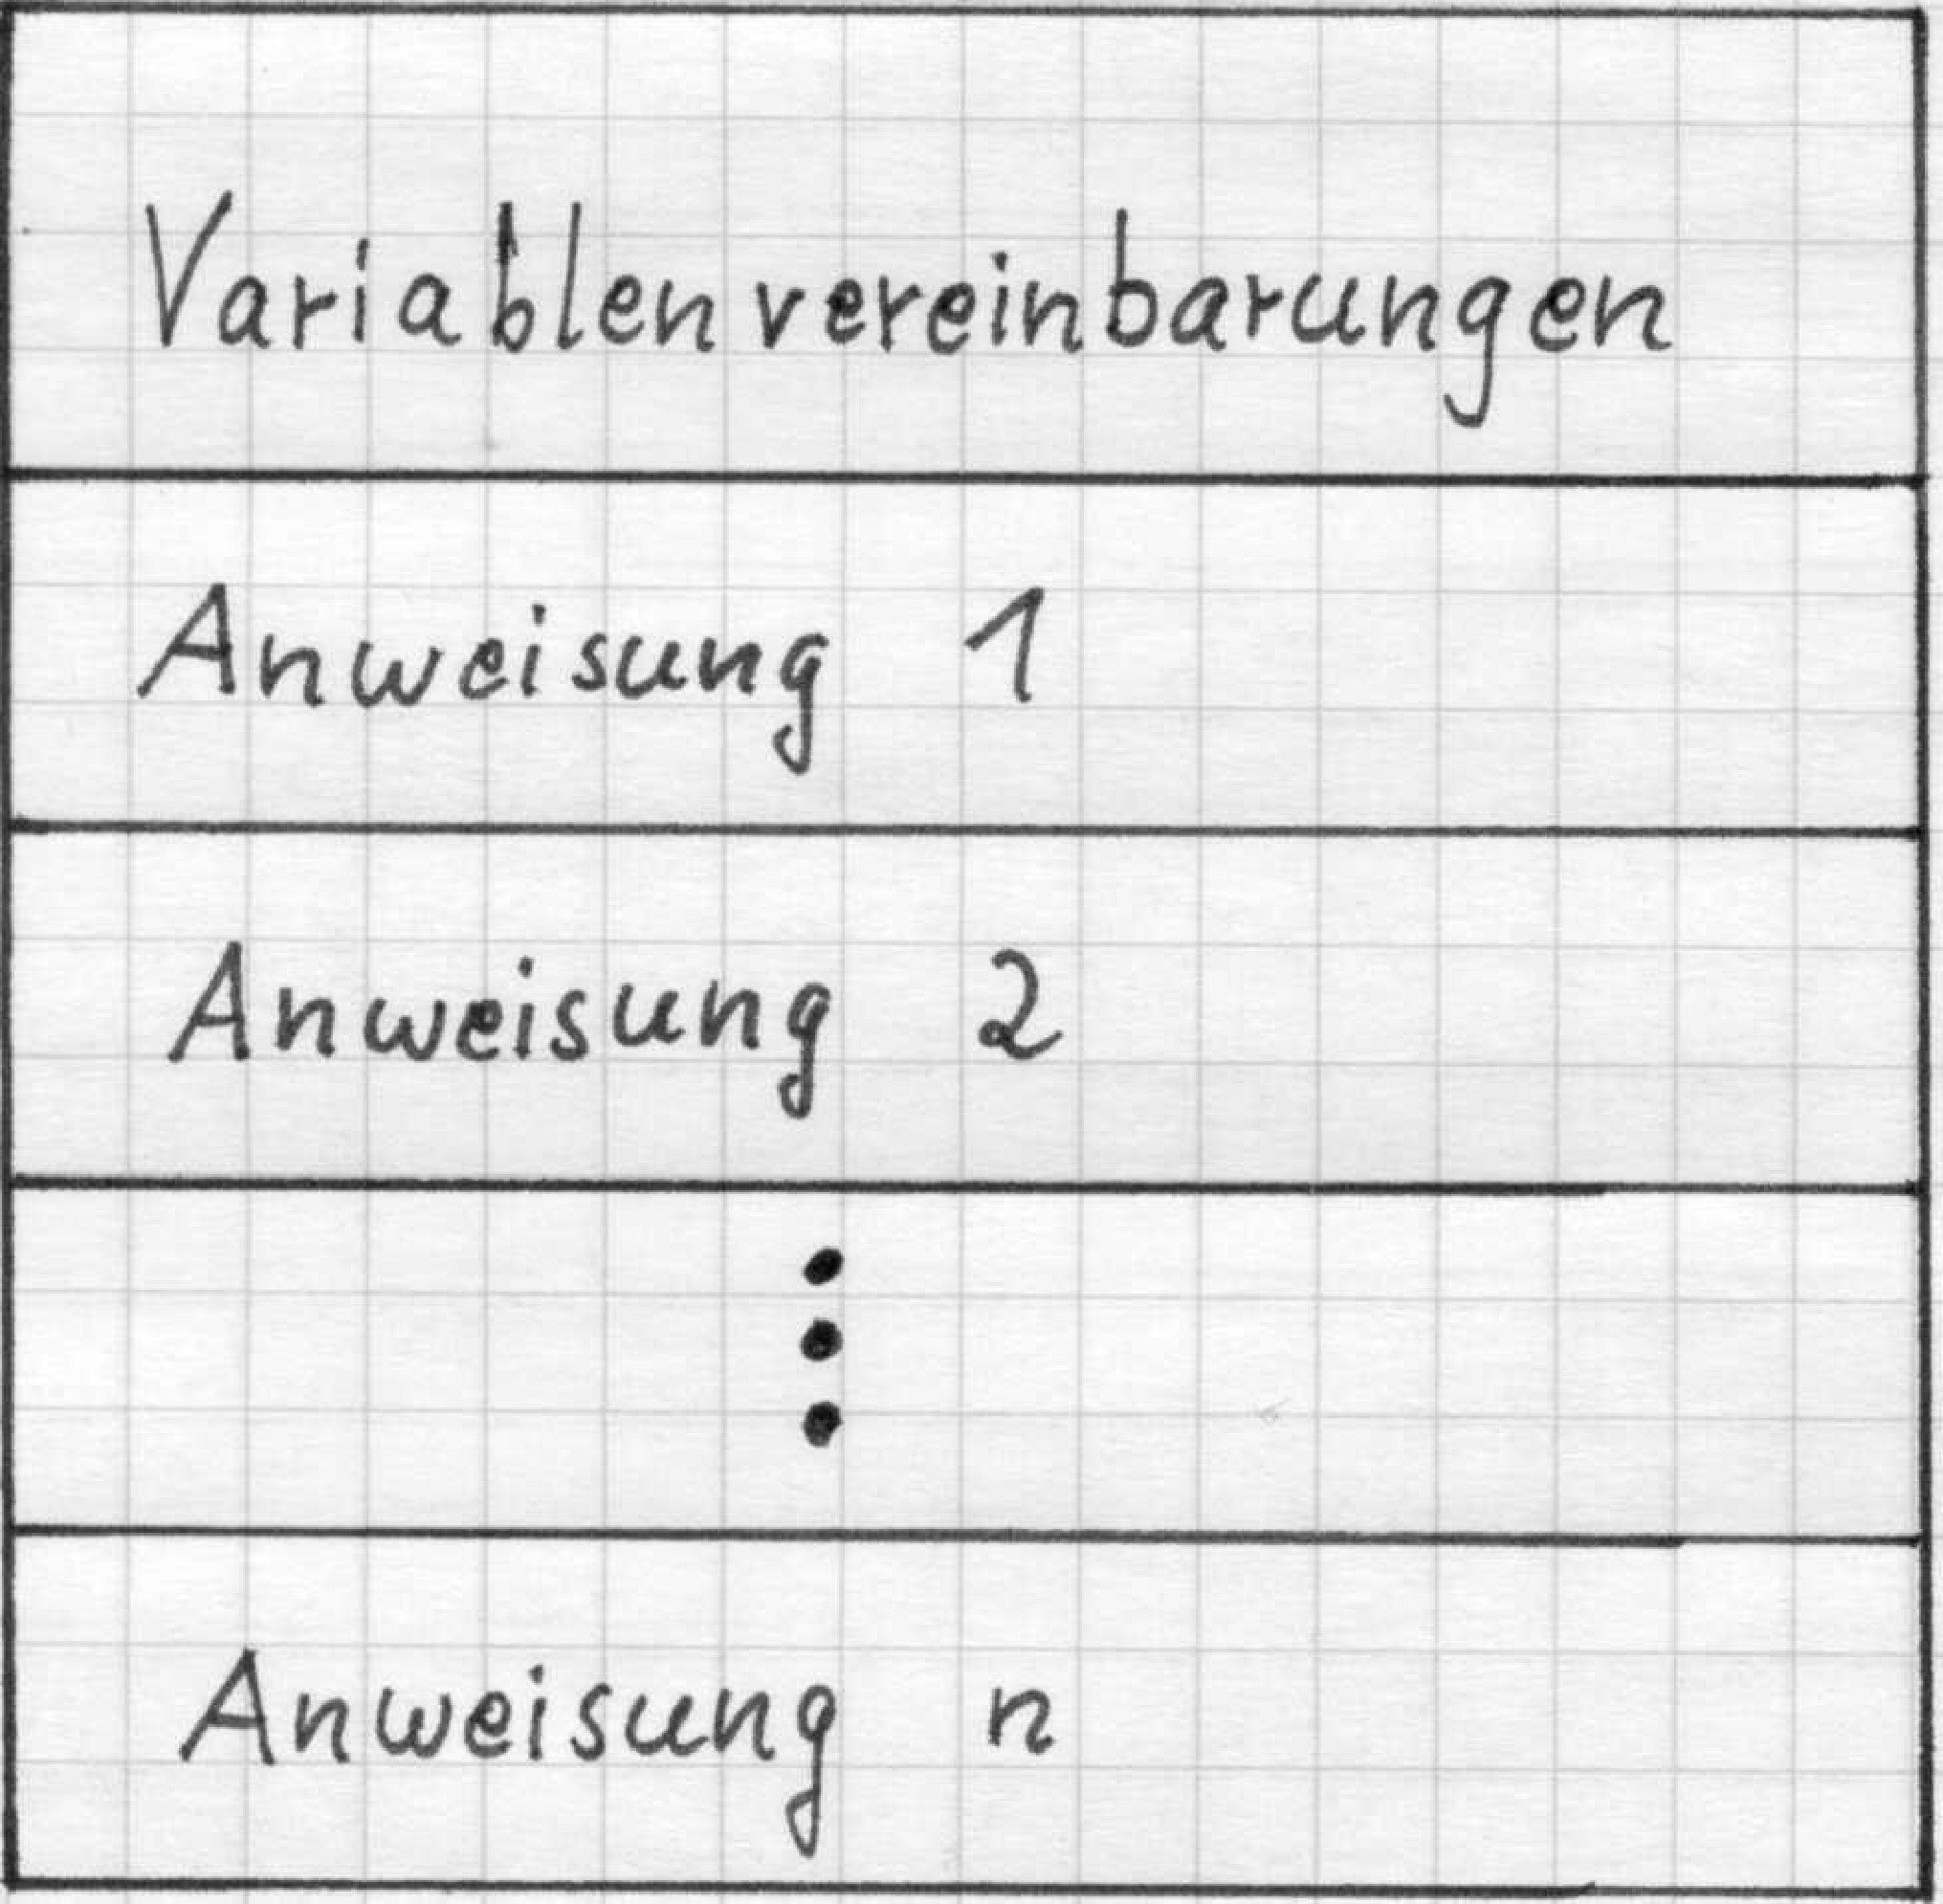
\includegraphics[scale=0.15]{GIF/p26}
%
\begin{itemize}
 \item
  In C {mu\ss} der Vereinbarungsteil dem Blockanfang direkt folgen.
  In C++ k"onnen mehrere Vereinbarungsteile im Block existieren, sie
  m"ussen nur vor der jeweiligen Erstbenutzung der Variablennamen stehen.
  Dies hat den Vorteil, da"s Variablen nur dort definiert (und initialisiert!!) werden m"ussen
  wo sie auch gebraucht werden.
 \item Der schlie{\ss}enden Klammer des Blockendes ``\}'' folgt kein
 	Semikolon.
 \item Ein Block kann stets anstelle einer Anweisung verwendet werden.
 \item Bl"ocke k"onnen beliebig ineinander  geschachtelt werden.
 \item Die in einem Block vereinbarten Variablen sind nur dort sichtbar,
 	d.h., au{\ss}erhalb des Blocks ist die Variable nicht existent
	(Lokalit"at). Umgekehrt kann auf Variablen des "ubergeordneten Blocks
	zugegriffen werden.\index{Block!Lokalit\"at}\index{scope}\index{Gültigkeitsbereich}
	%\exfile{Ex420.cpp}
\end{itemize}
\includecode[firstline=6]{Ex420.cpp}{Gültigkeitsbereich (scope) von Variablen}
%
Im Listing~\ref{lst:Ex420.cpp} tritt die Variable \texttt{i} sowohl im inneren
als auch im äußeren Block auf.
Dies nennt man \emph{shadow variable}, d.h., die innere Variable verdeckt die äußere.
Damit ist der Code schwerer zu verstehen und fehleranfälliger, ergo vermeiden Sie
shadow variables in Ihren Programmen.
Beim Gnu-Compiler warnt die Option \verb| -Wshadow | davor.
%
\section{Verzweigungen}
\label{p:4.3}
%
Die allgemeine Form der Verzweigungen (auch Alternative) ist
\index{Alternative}\index{Verzweigungen|see{Alternative}}
\index{if-then-else|see{Alternative}}

\mbox{}\hfill
\begin{minipage}[t]{0.6\textwidth}
\begin{verbatim}
if ( <logischer ausdruck> )
  <anweisung_A>
else
  <anweisung_B>
\end{verbatim}
\end{minipage}
\hfill\mbox{}

und z"ahlt ihrerseits wiederum als Anweisung. Der \verb|else|~-Zweig
kann weggelassen werden (einfache Alternative).

% \pagebreak[4]
\underline{Struktogramm}: \\
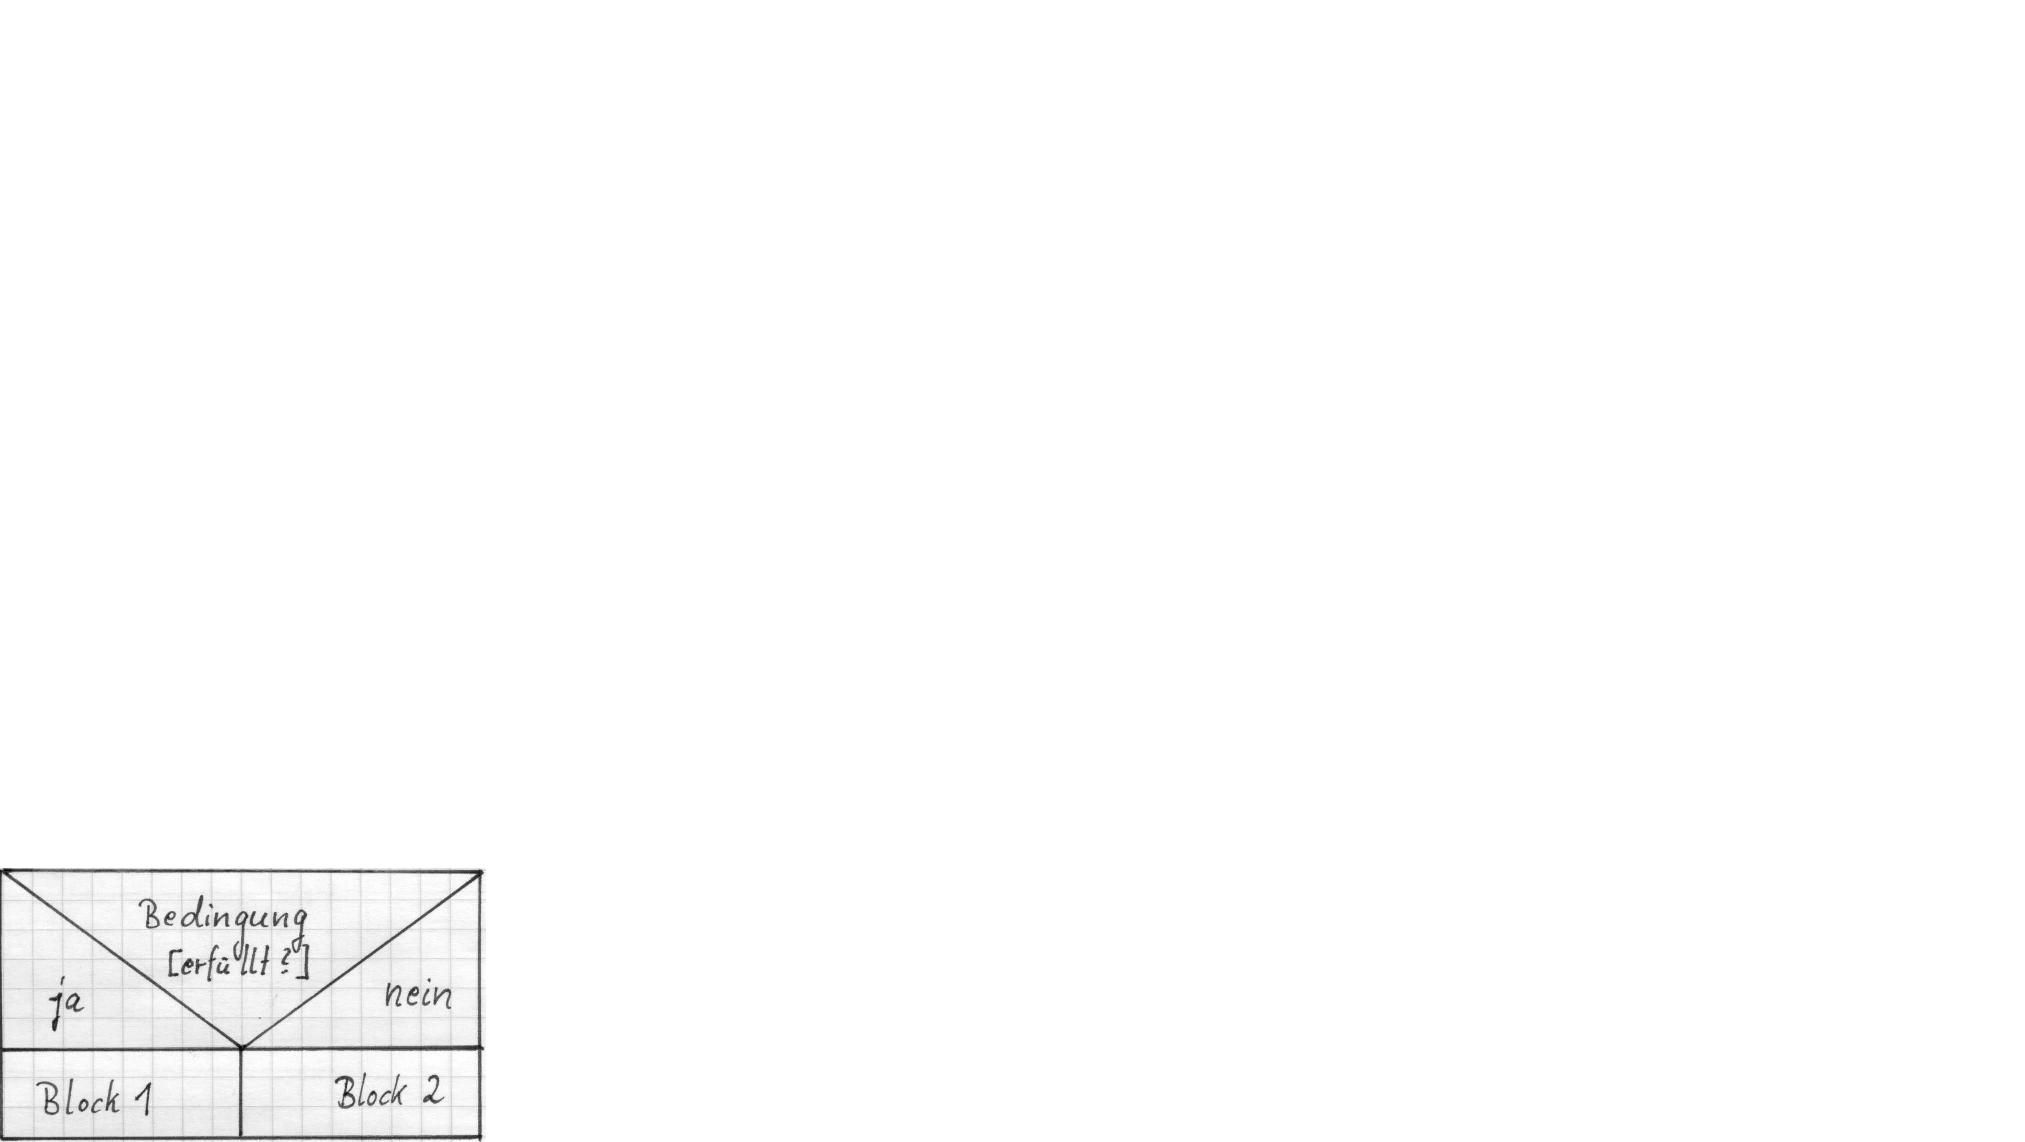
\includegraphics[scale=0.15]{GIF/p27.eps}
%

Wie so oft kann ein konkretes Problem auf verschiedene Weise
programmiert werden.
\\
\textbf{Beispiel}: Wir betrachten dazu die Berechnung der
Heaviside-Funktion\index{Heaviside}
$$
 y(x) = \begin{cases} 1 & \quad x \ge 0 \\ 0 & \quad x < 0 \end{cases}
$$
und stellen die folgenden vier Varianten der Implementierung vor.
%\exfile{Ex431.cpp}
\begin{enumerate}
	\renewcommand{\labelenumi}{\alph{enumi})}
	\item Setzen des Standardwertes kombiniert mit einer einfache Alternative,
	\item zweifache Alternative ohne Blöcke (da in jedem Zweig genau eine Anweisung steht),
	\item zweifache Alternative mit Blöcken (allgemeiner),
	\item mit dem Entscheidungsoperator.
	  Treten in einer zweifachen Alternative in jedem Zweig nur je eine
      Wertzuweisung zur selben Variablen auf (wie in Versionen b) und c)),
      dann kann der Entscheidungsoperator
      \\
     \centerline {\texttt{ <log.\  ausdruck> {\bf ?} <ausdruck\_A> {\bf :} <ausdruck\_B>  }}
\end{enumerate}
%
\includecode[firstline=7]{Ex431.cpp}{Vier Varianten um Heavisidefunktion zu implementieren}
%

\textbf{Beispiel}: Ein weiteres Beispiel ist die Berechnung
der Signum-Funktion (Vorzeichenfunktion)\index{Signum}
$$
 y(x) = \begin{cases} 1 & \quad x > 0 \\ 0 & \quad x = 0 \\ -1 & \quad x < 0 \end{cases}
$$
und wir stellen mehrere Varianten der Implementierung vor.
\bspfile{Ex432.cpp}
\label{bsp:sgn1}

\underline{Struktogramm}:\\
%
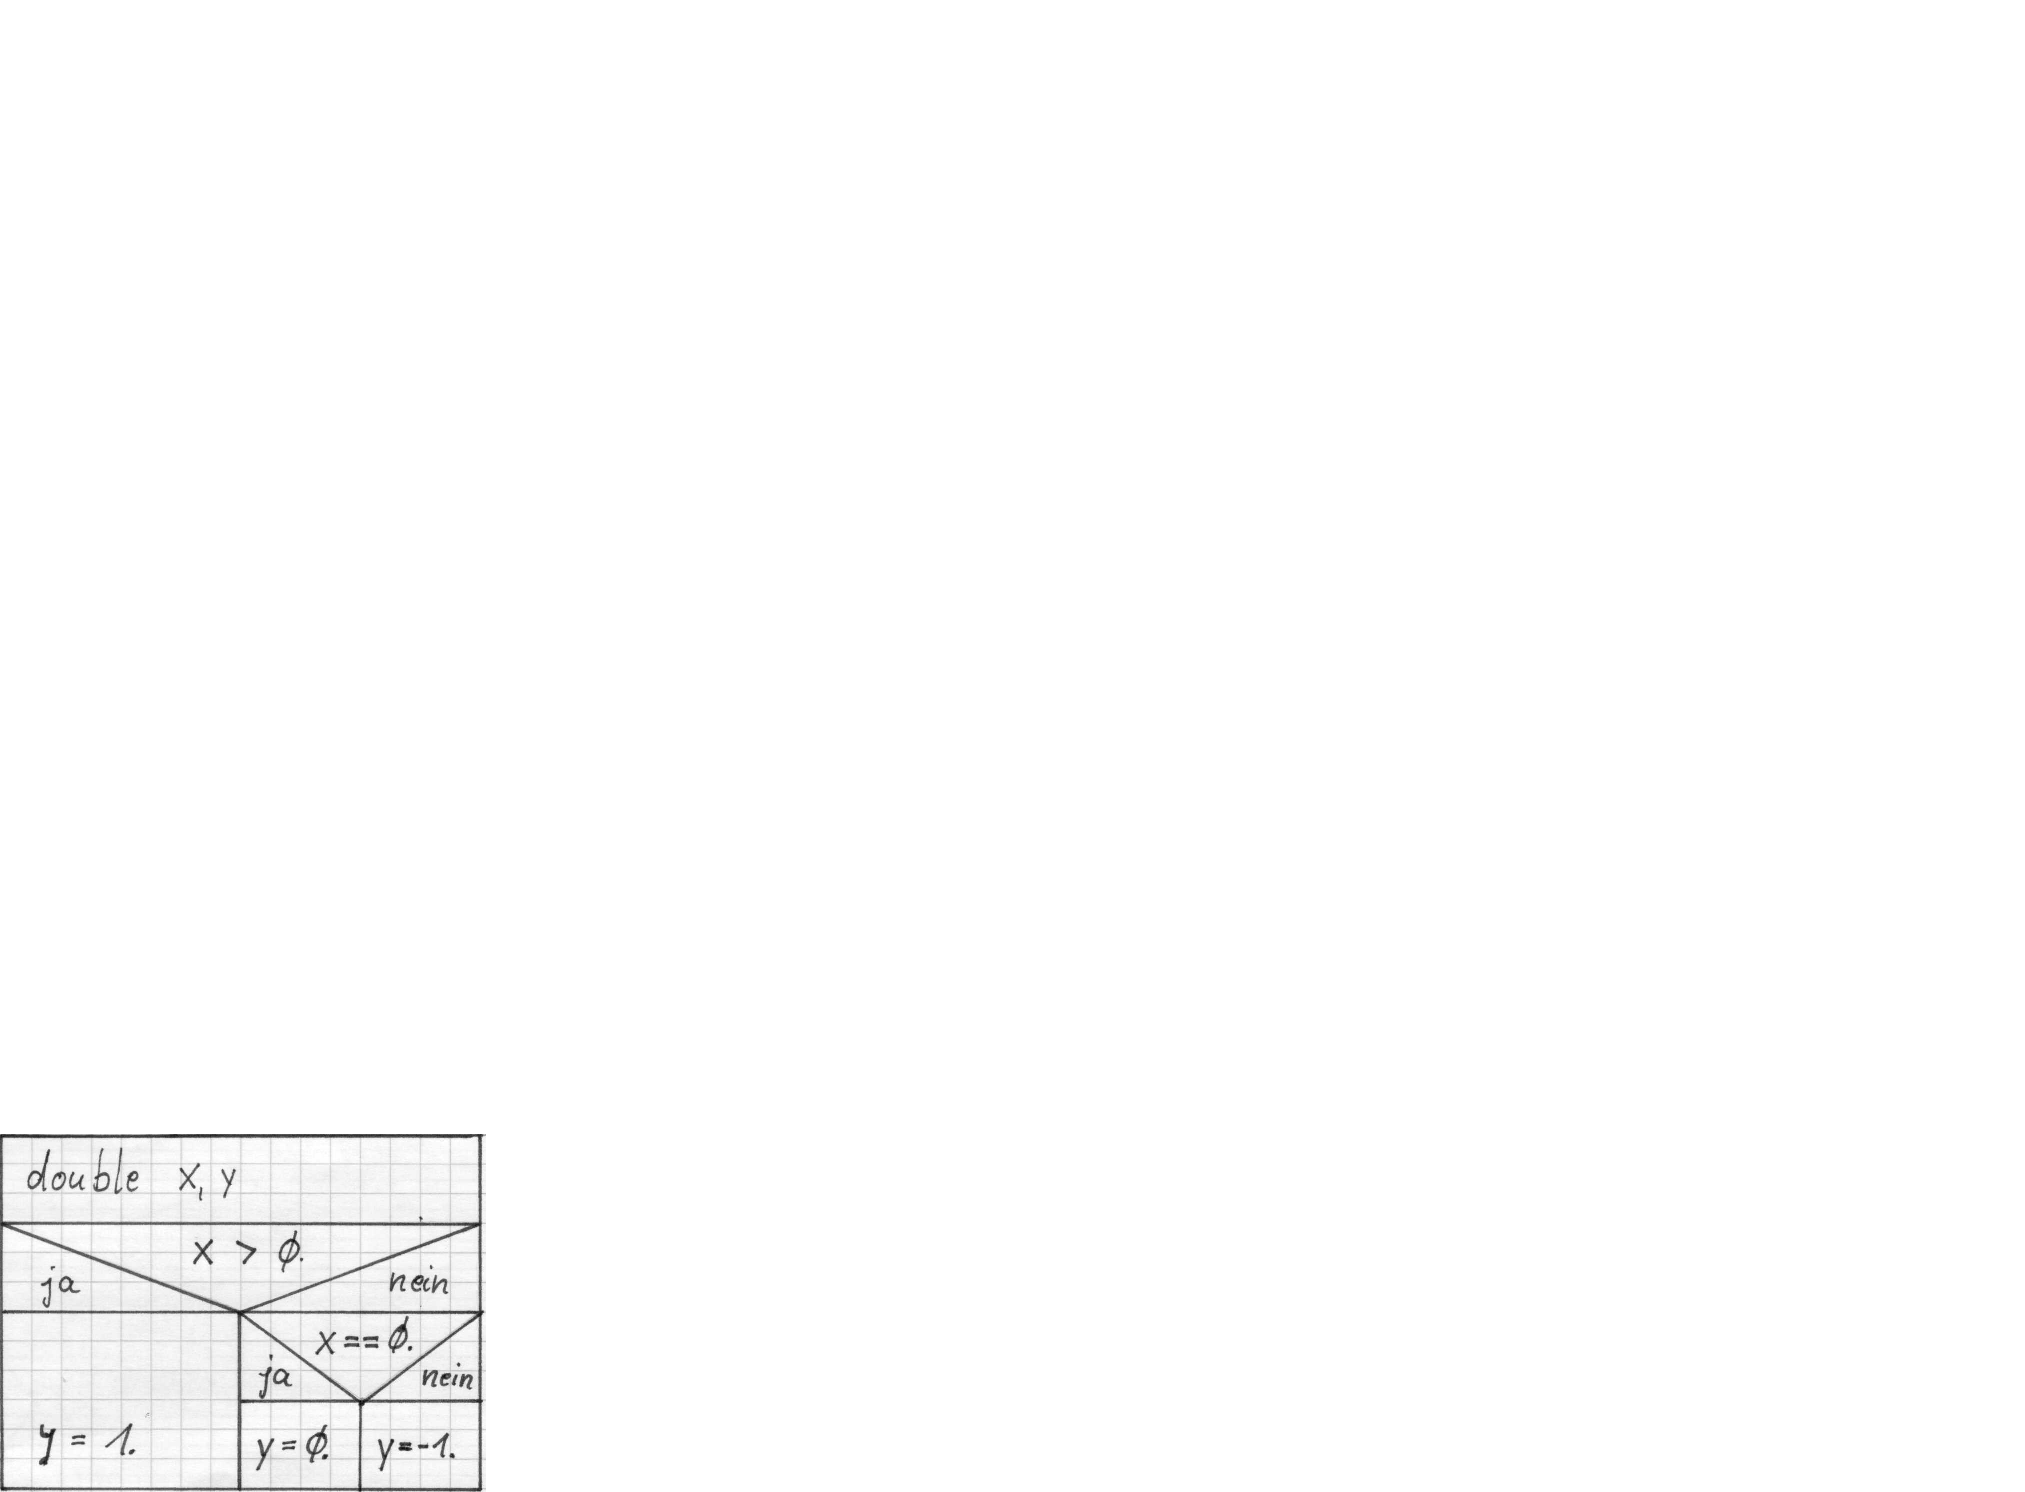
\includegraphics[scale=0.15]{GIF/p29.eps}
\\
%
Wir betrachten folgende Implementierungsvarianten:
\begin{enumerate}
	\renewcommand{\labelenumi}{\alph{enumi})}
	\item Schachtelung der Alternativen, d.h., der \verb|else|-Zweig enthält nochmals
	  eine Alternative.
	\item Falls der \verb|else|-Zweig nur aus einer
        weiteren \verb|if|-\verb|else|-Anweisung besteht, kann das  \verb|else| mit
        dem inneren \verb|if| zum \verb|elseif| kombiniert werden.
    \item Die Signumfunktion kann auch als Kombination von  zwei Heaviside-Funktionen
    ausgedrückt werden und damit als Kombination zweier Entscheidungsoperatoren
    implementiert werden (kurz und knapp, aber aus dem Code nur schwer zu verstehen).
\end{enumerate}
%
\includecode[firstline=7]{Ex432.cpp}{Drei Varianten der Signum-Funktion}
%

% \newpage
\begin{samepage}
Allgemein kann eine solche Mehrwegentscheidung als
\\[1ex]
\mbox{}\hfill
\begin{minipage}[t]{0.7\textwidth}
\begin{verbatim}
if ( <logischer ausdruck_1> )
  <anweisung_1>
else if ( <logischer ausdruck_2> )
  <anweisung_2>
        ...
else if ( <logischer ausdruck_(n-1)> )
  <anweisung_(n-1)>
else
  <anweisung_n>
\end{verbatim}
\end{minipage}
\hfill\mbox{}\label{mehrweg}
\\[1ex]
geschrieben werden, wobei der \verb|else|-Zweig wiederum optional ist.
\end{samepage}

\pagebreak{}
\begin{samepage}
\textbf{Beispiel}: Bestimmung von Minimum und Maximum
zweier einzugebender Zahlen.

\underline{Struktogramm}: \\
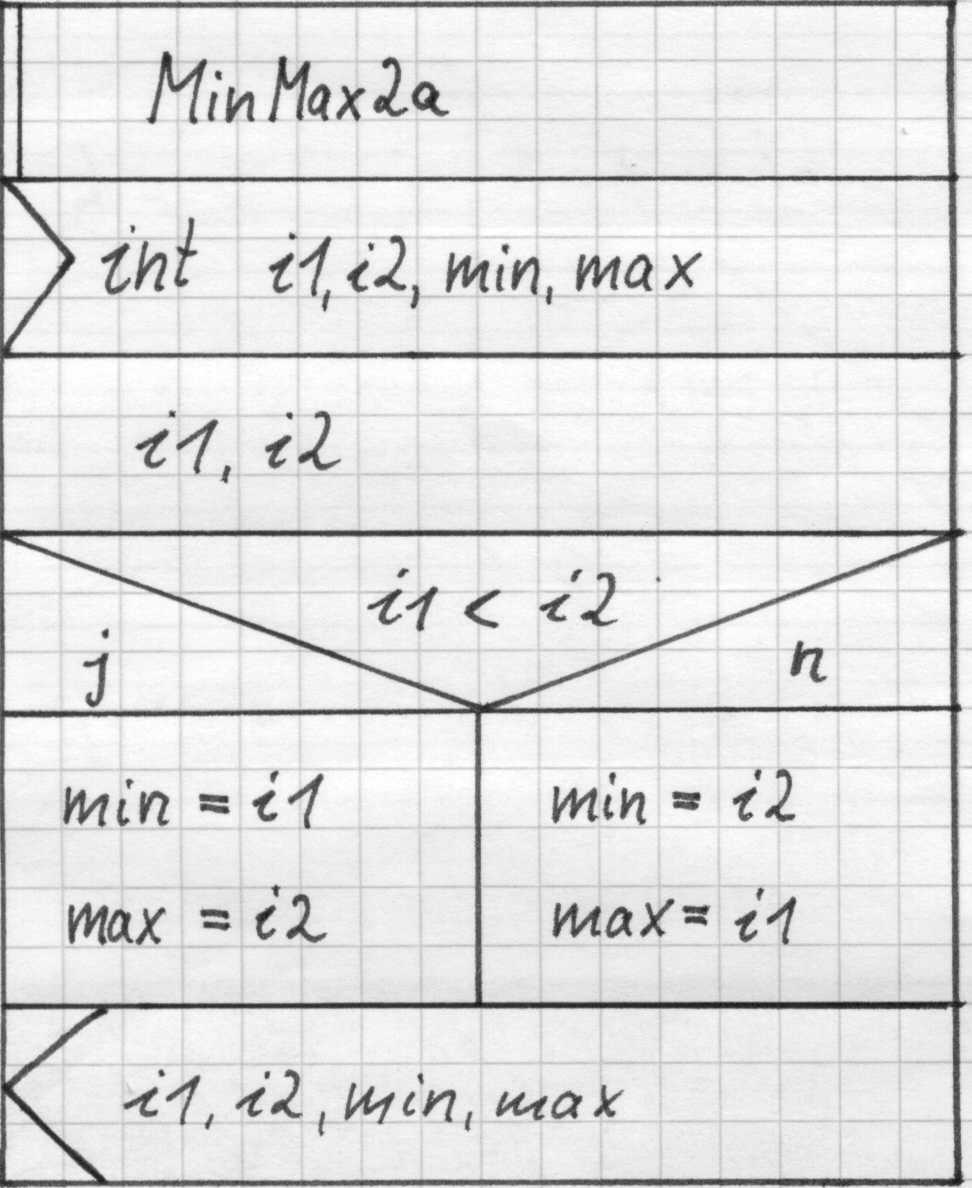
\includegraphics[scale=0.15]{GIF/p31a.eps}
\end{samepage}
\includecode[firstline=7]{Ex433.cpp}{Drei Varianten das Minimum und das Maximum zweier Zahlen zu bestimmen}
%
Die Funktionen \texttt{min} und \texttt{max} zur Bestimmung des Minimus/Maximums zweier Zahlen
sind in der STL (Standard Template Library) bereits implementiert,\index{STL}
somit lassen sich alle 3~Varianten auch durch
\verb| imax = max(i1,i2); imin = min(i1,i2); |
ausdrücken.

\pagebreak
\textbf{Beispiel}: Bestimmung des Minimums
dreier einzugebender Zahlen.
%\exfile{Ex434.cpp}

\underline{Struktogramm}: \\%[4cm]
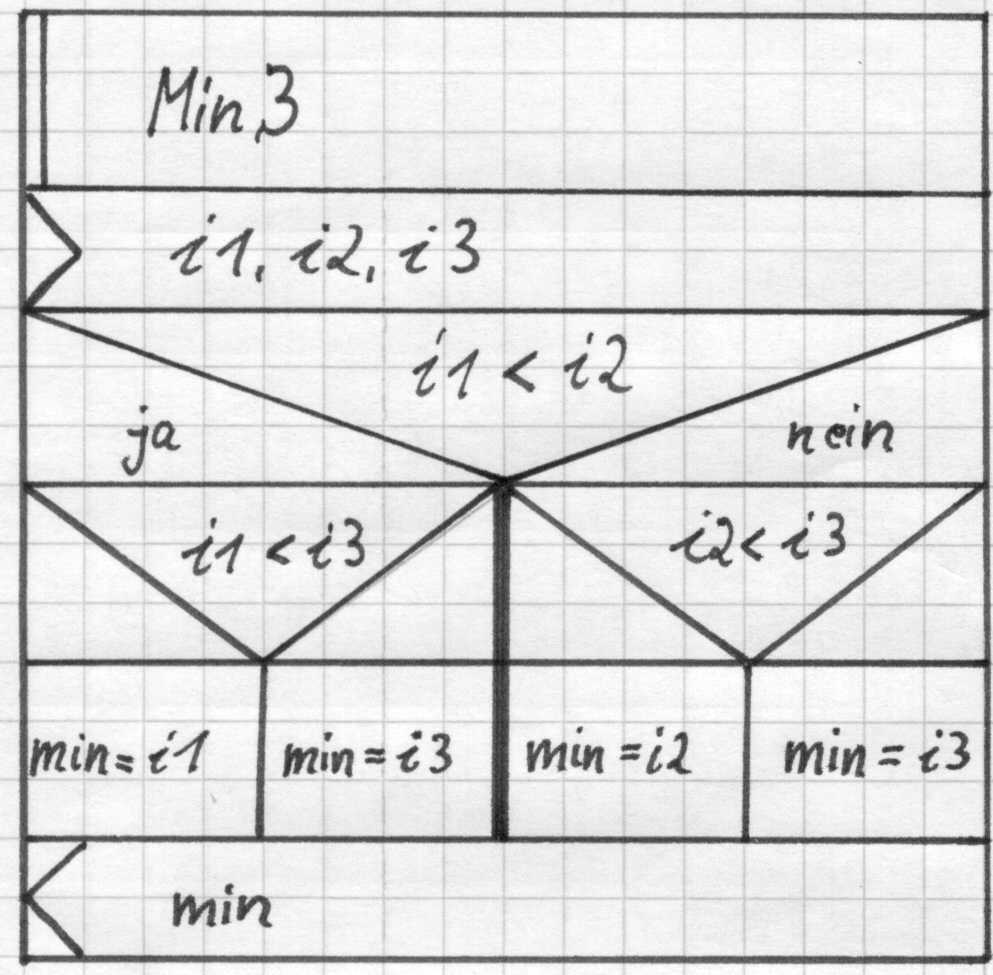
\includegraphics[scale=0.15]{GIF/p32.eps}
%
\includecode[firstline=7]{Ex434.cpp}{Varianten des Minimums dreier Zahlen}
%
%
%
\section[Der Z"ahlzyklus]{Der Z"ahlzyklus (\texttt{for}-Schleife)}
\label{p:4.4}
%
Beim Z"ahlzyklus steht die Anzahl der Zyklendurchl"aufe
\textbf{a-priori} fest, der Abbruchtest erfolgt vor dem Durchlauf eines Zyklus.
Die allgemeine Form ist
\index{Z\"ahlzyklus}\index{for-Schleife|see{Z\"ahlzyklus}}

\mbox{}\hfill
\begin{minipage}[t]{0.8\textwidth}
\begin{verbatim}
for (<ausdruck_1>; <ausdruck_2>; <ausdruck_3>)
  <anweisung>
\end{verbatim}
\end{minipage}
\hfill\mbox{}
%\newpage
Am besten sei der Z"ahlzyklus an einem Beipiel erl"autert.
%\newpage

\textbf{Beispiel}: Es ist die Summe der ersten 5 nat"urlichen
Zahlen zu berechnen: $\displaystyle isum = \sum_{i=1}^{5} i$.
%
\includecode[firstline=7]{Ex440.cpp}{Summe der ersten 5 natürlichen Zahlen}

Im obigen Programmbeispiel ist \verb|i| die
Laufvariable\index{Laufvariable} des Z"ahlzyklus,
welche mit \verb|i = 1| (\verb|<ausdruck_1>|) initialisiert, mit
\verb|i = i+1| (\verb|<ausdruck_3>|) weitergez"ahlt und in
\verb|i <= n| (\verb|<ausdruck_2>|) bzgl.\  der
oberen Grenze der Schleifendurchl"aufe getestet wird.
Im Schleifeninneren \verb|sum = sum + i;| (\verb|anweisung|) erfolgen die
eigentlichen Berechnungsschritte des Zyklus. Die  Summationsvariable
\verb|sum| {mu\ss} vor dem Eintritt in den Zyklus initialisiert werden.

Eine kompakte Version dieser Summationsschleife
(korrekt, aber sehr schlecht lesbar) w"are :
\\
\verb|for (isum = 0, int i = 1; i <= n; isum += i, ++i)|
\\
Man unterscheidet dabei zwischen dem Abschlu{\ss} einer Anweisung ``\verb|;|''
und dem Trennzeichen ``\verb|,|'' in einer Liste von Ausdr"ucken.
Diese Listen werden von links nach rechts abgearbeitet.

Der \verb|<ausdruck_2>| ist stets ein logischer Ausdruck
(\S~\ref{p:3.3}-\ref{p:3.4}) und \verb|<ausdruck_3>|
ist ein arithmetischer Ausdruck zur Manipulation der Laufvariablen,
z.B.\\[1ex]
\begin{minipage} {0.9\textwidth}
\begin{verbatim}
 ++i
 j = j-2
 j += 2
 x = x+h         // float-Typ
 k = 2*k         // Verdoppelung
 l = l/4         // Viertelung - Vorsicht bei Integer
\end{verbatim}
\end{minipage}

%\pagebreak[4]
\underline{Struktogramm}: \\
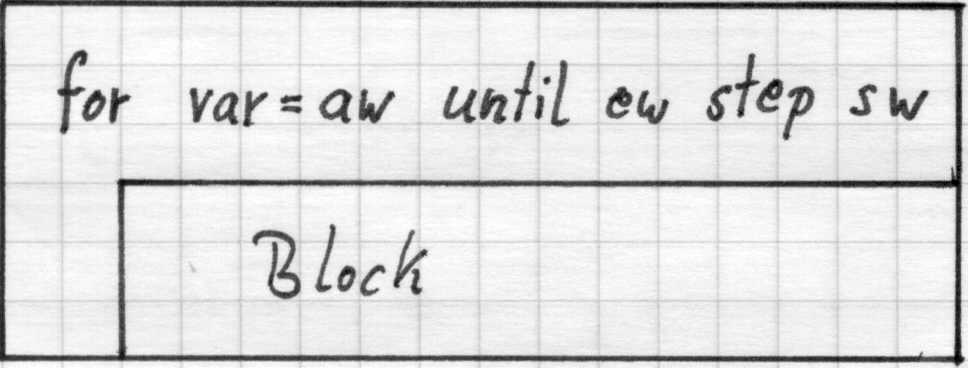
\includegraphics[scale=0.15]{GIF/p34.eps}
%
\begin{itemize}
 \item Die Laufvariable mu"s eine einfache Variable aus \S~\ref{p:2.2}
 	sein, z.B., \verb|int| oder \verb|double|,\index{Laufvariable}
	oder ein Iterator~\S~\ref{p:6.3} (auch Pointer).
 \item Vorsicht bei Verwendung von Gleitkommazahlen
 (\verb|float|, \verb|double|) als\bspfile{Loop_Float.cpp}
 Laufvariable.\index{Laufvariable!Gleitkommazahl}\index{Gleitkommazahl!Laufvariable}
 Dort ist der korrekte Abbruchtest wegen der internen Zahldarstellung
 u.U.\  nicht einfach zu realisieren.\index{Z\"ahlzyklus!Abbruchtest}
\end{itemize}


\begin{minipage}[c]{0.4\textwidth}
\textbf{Beispiel}:
Es sei die Doppelsumme
$$
  \text{sum} = \sum_{k=1}^n \underbrace{\sum_{i=1}^k \frac{1}{i^2}}_{t_k}
  =  \sum_{k=1}^n t_k
$$
f"ur einzugebende $n$ zu berechnen.\\
\textbf{Hinweis:} F"ur die innere Summe gilt $t_k = t_{k-1}+1/k^2$
f"ur $k=1,\ldots,n$ mit $t_0 = 0$. Dadurch f"allt diese kostspielige
Summation weg wodurch der gesamte Code signifikant schneller wird
%% \htmladdnormallink{\textit{Ex442fast.cpp}}{\url{../../Examples/Ex442fast.cpp}}).
%%(\htmladdnormallink{\textit{Ex442fast.cpp}}{../../Examples/Ex442fast.cpp}).%
\footnote{Andere M"oglichkeit:
Vertauschen der Summationen $\sum_{i=1}^n \sum_{k=i}^n \frac{1}{i^2}
 =  \sum_{i=1}^n  \frac{n-i+1}{i^2}$ [A. Reinhart]}
\end{minipage}\bspfile{Ex442fast.cpp}
%
%
% weitere Variante: Hr. Andreas Reinhart
%
% vertauschen der Summen:
% $
% \text{sum} = \sum_{i=1}^n \sum_{k=i}^n \frac{1}{i^2}
% =  \sum_{i=1}^n  \frac{n-i+1}{i^2}
% $
%
%
\hfill
\begin{minipage}{0.5\textwidth}
\underline{Struktogramm}: \\
%
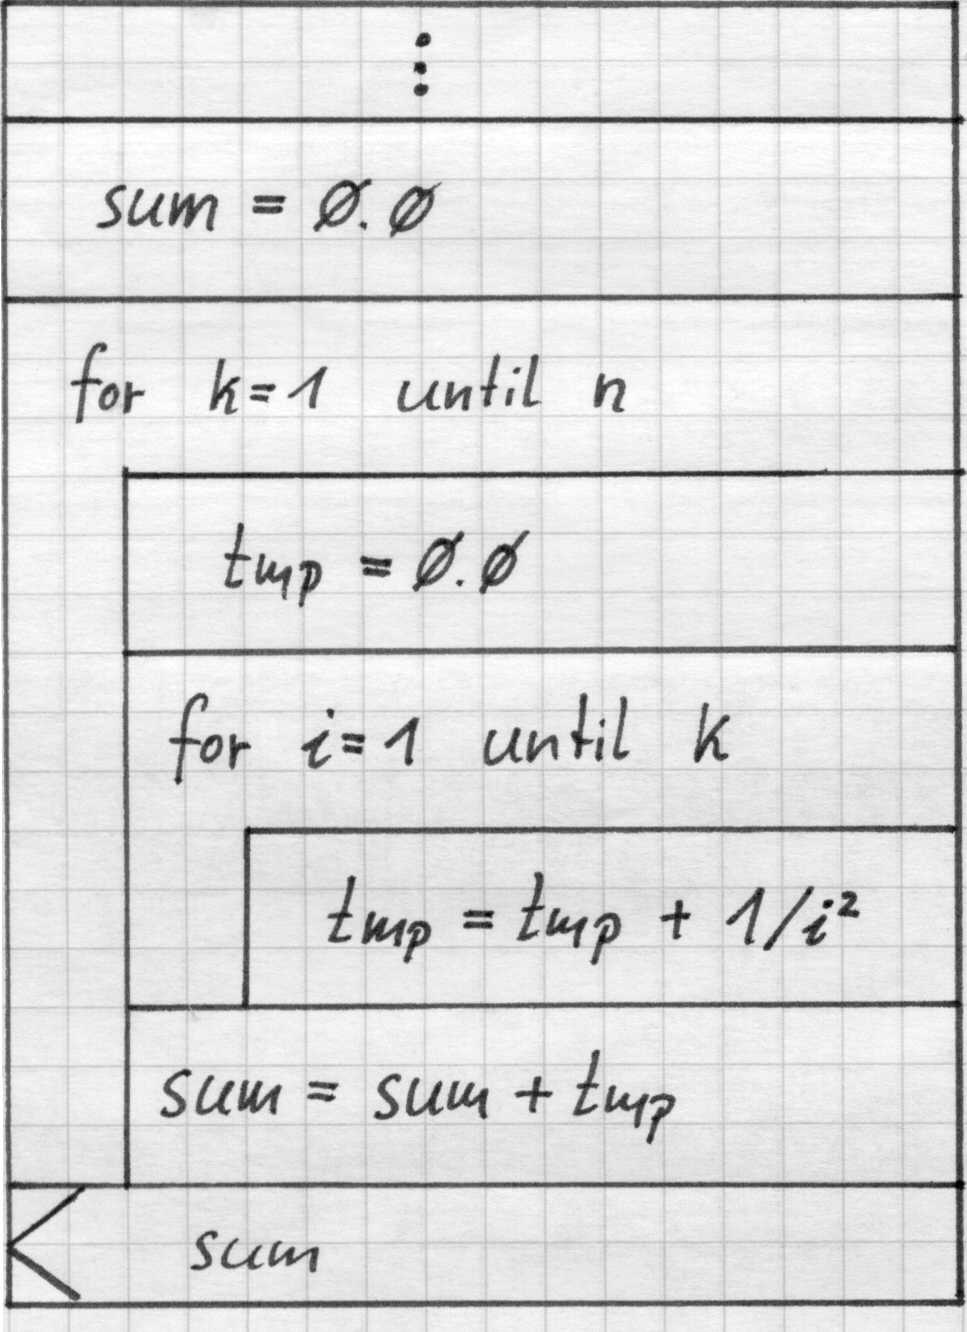
\includegraphics[scale=0.15]{GIF/p35.eps}
\end{minipage}
%
\includecode[firstline=7]{Ex442.cpp}{Geschachtelte Zählzyklen}
%

Weitere einfache \textbf{Beispiele} berechnen die Summe der
ersten geraden nat"urlichen Zahlen
\bspfile{Ex443.cpp}
und das Z"ahlen eines CountDowns.
\bspfile{Ex444.cpp}

%
%				woanders einbauen ?
%
Die folgenden Beispiele verdeutlichen die Problematik der
begrenzten Genauigkeit von Gleitkommazahlen in Verbindung
mit Zyklen und einige Tips zu deren Umgehung.\index{Gleitkommazahl!Genauigkeit}

% %\pagebreak
% \textbf{Beispiel:} Ausgabe der St"utzpunkte $x_i$ des Intervalls~$[0,1]$,
% welches in $n$~gleichgro"se Teilintervalle zerlegt wird, d.h.,
% \bspfile{Loop\_Float.cpp}
% $$
%  x_i = i \cdot h \quad,\;i=0,\ldots,n\qquad\text{mit } h = \frac{1-0}{n}
% $$
% \underline{Struktogramm}: \\
% \begin{latexonly}
% \special{psfile=GIF/p36b.eps.gz
% 	 hscale=15 vscale=15
% 	 voffset=-90
% 	}
% \\[3cm]
% \end{latexonly}
% \htmladdimg{p36b_4.jpg}{}
\begin{minipage}{0.4\textwidth}
\underline{Struktogramm}: \\
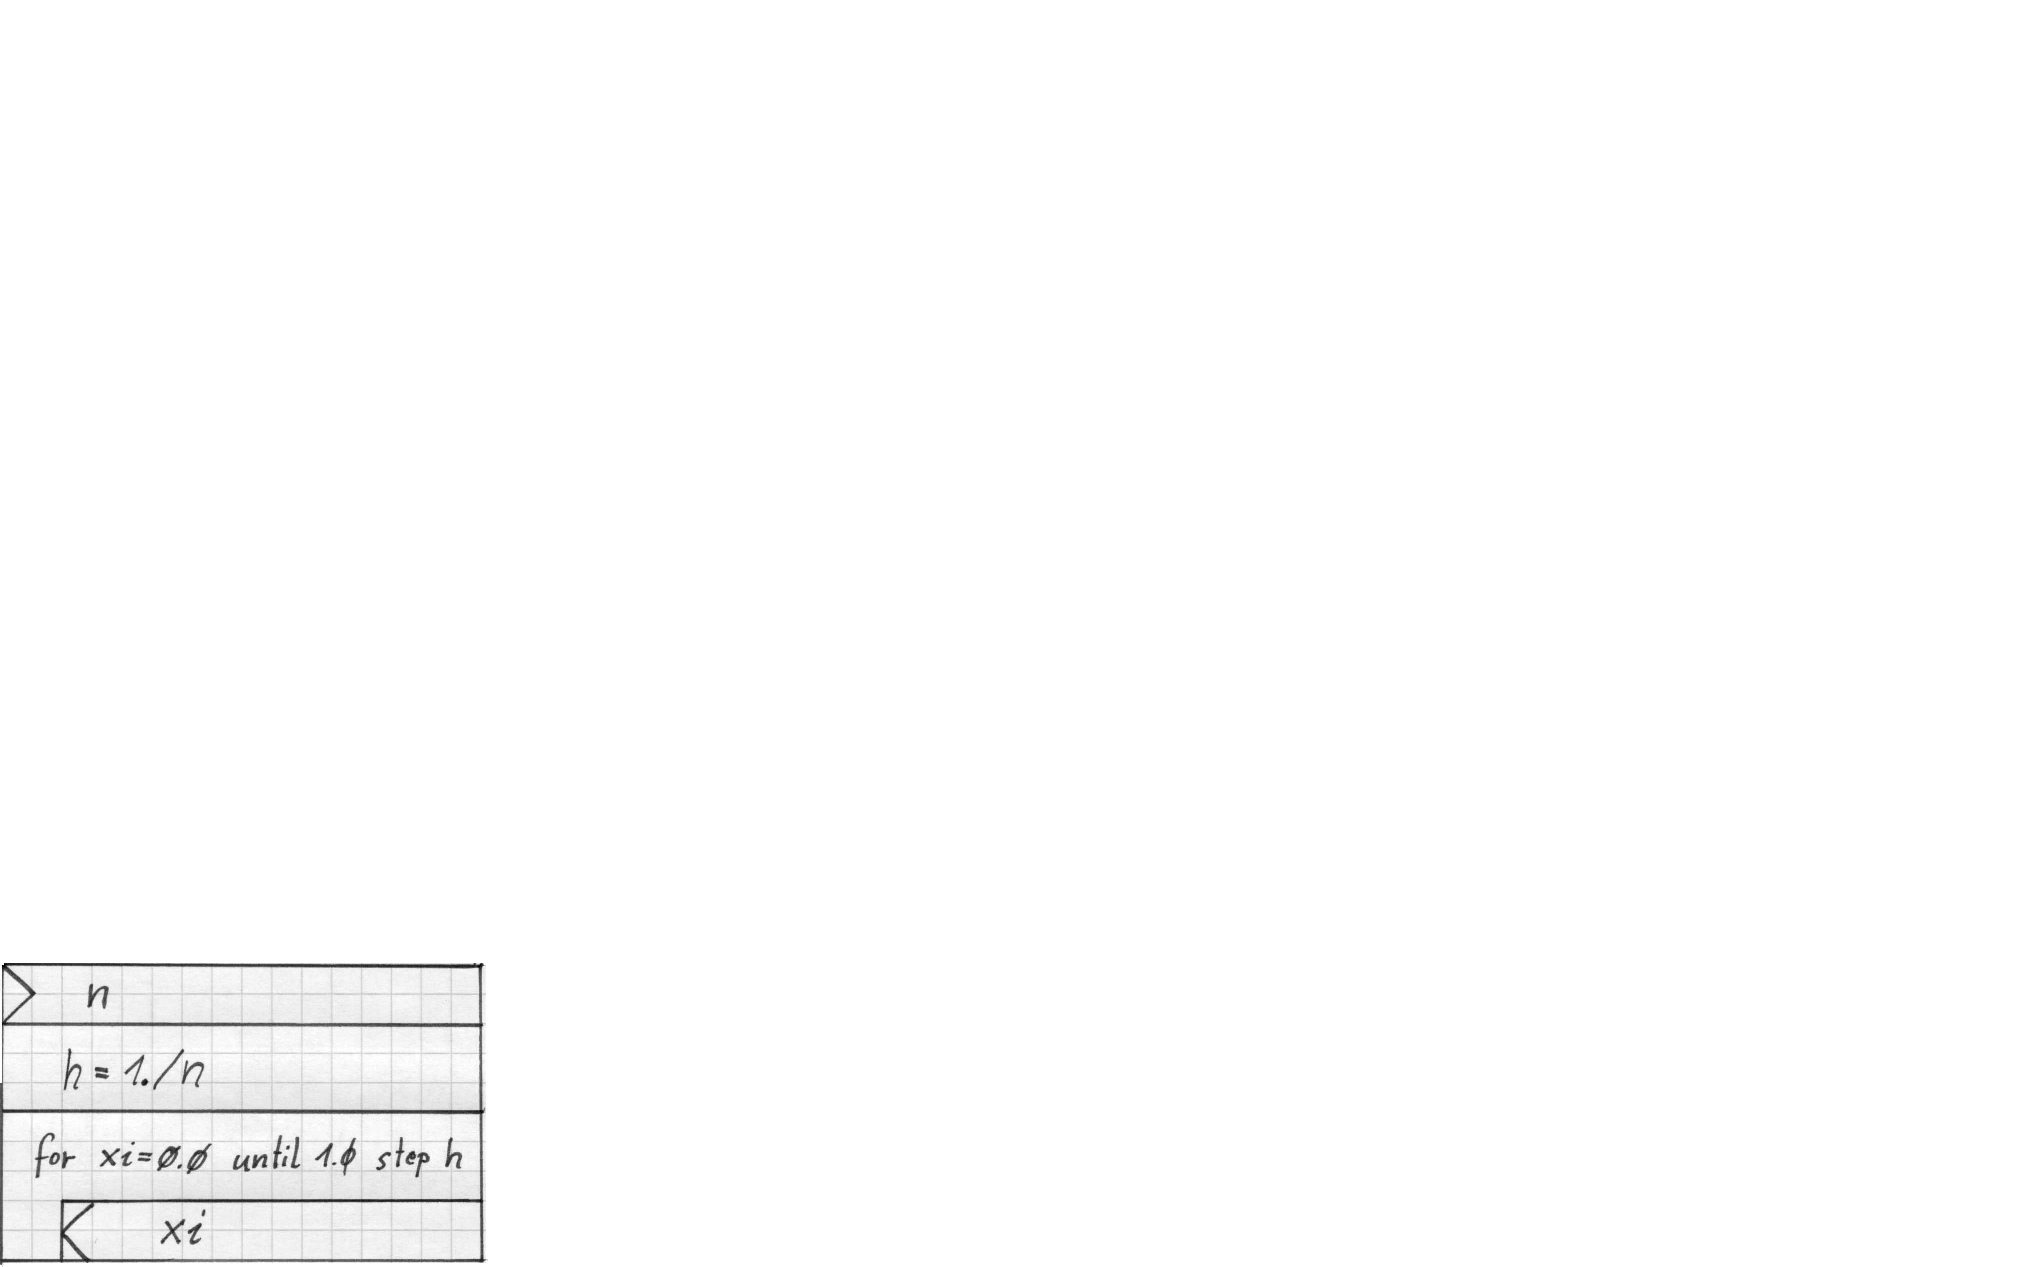
\includegraphics[scale=0.15]{GIF/p36b.eps}
\end{minipage}
%
\begin{minipage}{0.5\textwidth}
\textbf{Beispiel:} Ausgabe der St"utzpunkte $x_i$ des Intervalls~$[0,1]$,
welches in $n$~gleichgro"se Teilintervalle zerlegt wird, d.h.,
$$
 x_i = i \cdot h \quad,\;i=0,\ldots,n\qquad\text{mit } h = \frac{1-0}{n}
$$
\end{minipage}\bspfile{Loop\_Float.cpp}
%
% \pagebreak[4]
\includecode[linerange={7-8,11-17,33-38,41-42}]{Loop_Float.cpp}
{Aufpassen bei Zählzyklen mit Gleikommagröße als Laufvariable}
%
Da Gleitkommazahlen nur eine limitierte Anzahl g"ultiger Ziffern besitzen,
kann es (oft) passieren, da"s der letzte Knoten $x_n$ nicht
ausgegeben wird. Nur f"ur $n=2^k\;,\,k\in {\mathbb{N}}\;,\;k<32$ kann in unserem
Beispiel eine korrekte Abarbeitung des Z"ahlzyklus garantiert werden.
Auswege sind: 
\begin{enumerate}
 \item "Anderung des Abbruchtests in \verb| xi <= xe + h/2.0 |, jedoch
 	ist $x_n$ immer noch fehlerbehaftet. \\[1ex]
%
\begin{minipage} {0.5\textwidth}
\begin{verbatim}
 for (xi = xa; xi <= xe + h/2.0; xi += h)
   {
    cout << xi << endl;
   }
\end{verbatim}
\end{minipage}
 \item Besser ist ein Zählzyklus mit einer \verb|int|-Laufvariable wodurch
    die Werte $x_{i} = i \cdot h$ für große~$i$ genauer sind als in Variante~1.
    \\[2ex]
\nopagebreak
\begin{minipage} {0.5\textwidth}
\begin{verbatim}
 for (i = 0; i <= n; ++i)
   {
    xi = xa + i*h;
    cout << xi << endl;
   }
\end{verbatim}
\end{minipage}
\end{enumerate}

%\pagebreak
Die gemeinsame Summation kleinerer und gr"o"serer Zahlen kann ebenfalls zu
Ungenauigkeiten f"uhren. Im \textbf{Beispiel} wird
die Summe $s1:=\sum\limits_{i=1}^{n} 1/i^2$ mit
der (theoretisch identischen) Summe $s2:=\sum\limits_{i=n}^{1} 1/i^2$
f"ur gro"se $n$ ($65.000$, $650.000$) verglichen.
%
\includecode[linerange={7-8,10-13,21-29,33-40,51-52}]{Reihe.cpp}
{Auslöschung bei Summation kleiner Zahlen}
%
\index{cmath!ceil()}\index{numeric\_limits!epsilon}\index{numeric\_limits}

Das numerische Resultat in $s2$ ist genauer, da dort zuerst alle kleinen
Zahlen addiert werden, welche bei $s1$
wegen der beschr"ankten Anzahl g"ultiger Ziffern
keinen Beitrag zur Summation mehr liefern k"onnen.
Gleichzeitig ist zu beachten, da"s die Berechnung
von \verb| 1.0/(i*i) | in einem "Uberlauf endet, da \verb| i*i |
nicht mehr in \verb|int|-Zahlen darstellbar ist.
Dagegen erfolgt die Berechnung von \verb| 1.0/i/i |
vollst"andig im Bereich der Gleitkommazahlen.\index{Gleitkommazahl!\"Uberlauf}
%
%
%
\pagebreak
\section[Abweisender Zyklus]{Abweisender Zyklus (\texttt{while}-Schleife)}
\label{p:4.5}
%
Beim abweisenden Zyklus steht die Anzahl der Durchl"aufe nicht
a-priori fest, der Abbruchtest erfolgt \textbf{vor} dem Durchlauf eines Zyklus.
\index{abweisender Zyklus}\index{while-Schleife|see{abweisender Zyklus}}
\index{abweisender Zyklus!Abbruchtest}

% Die allgemeine Form ist
% 
% \mbox{}\hfill
% \begin{minipage}[t]{0.6\textwidth}
% \begin{verbatim}
% while (<logischer ausdruck>)
%   <anweisung>
% \end{verbatim}
% \end{minipage}
% \hfill\mbox{}

\begin{minipage}[t]{0.5\textwidth}
Die allgemeine Form ist\\[1ex]
\phantom{XXX}\verb|while (<logischer ausdruck>)| \\
\phantom{XXX}\verb|    <anweisung>|
\end{minipage}
\begin{minipage}[t]{0.4\textwidth}
\underline{Struktogramm}: %\\
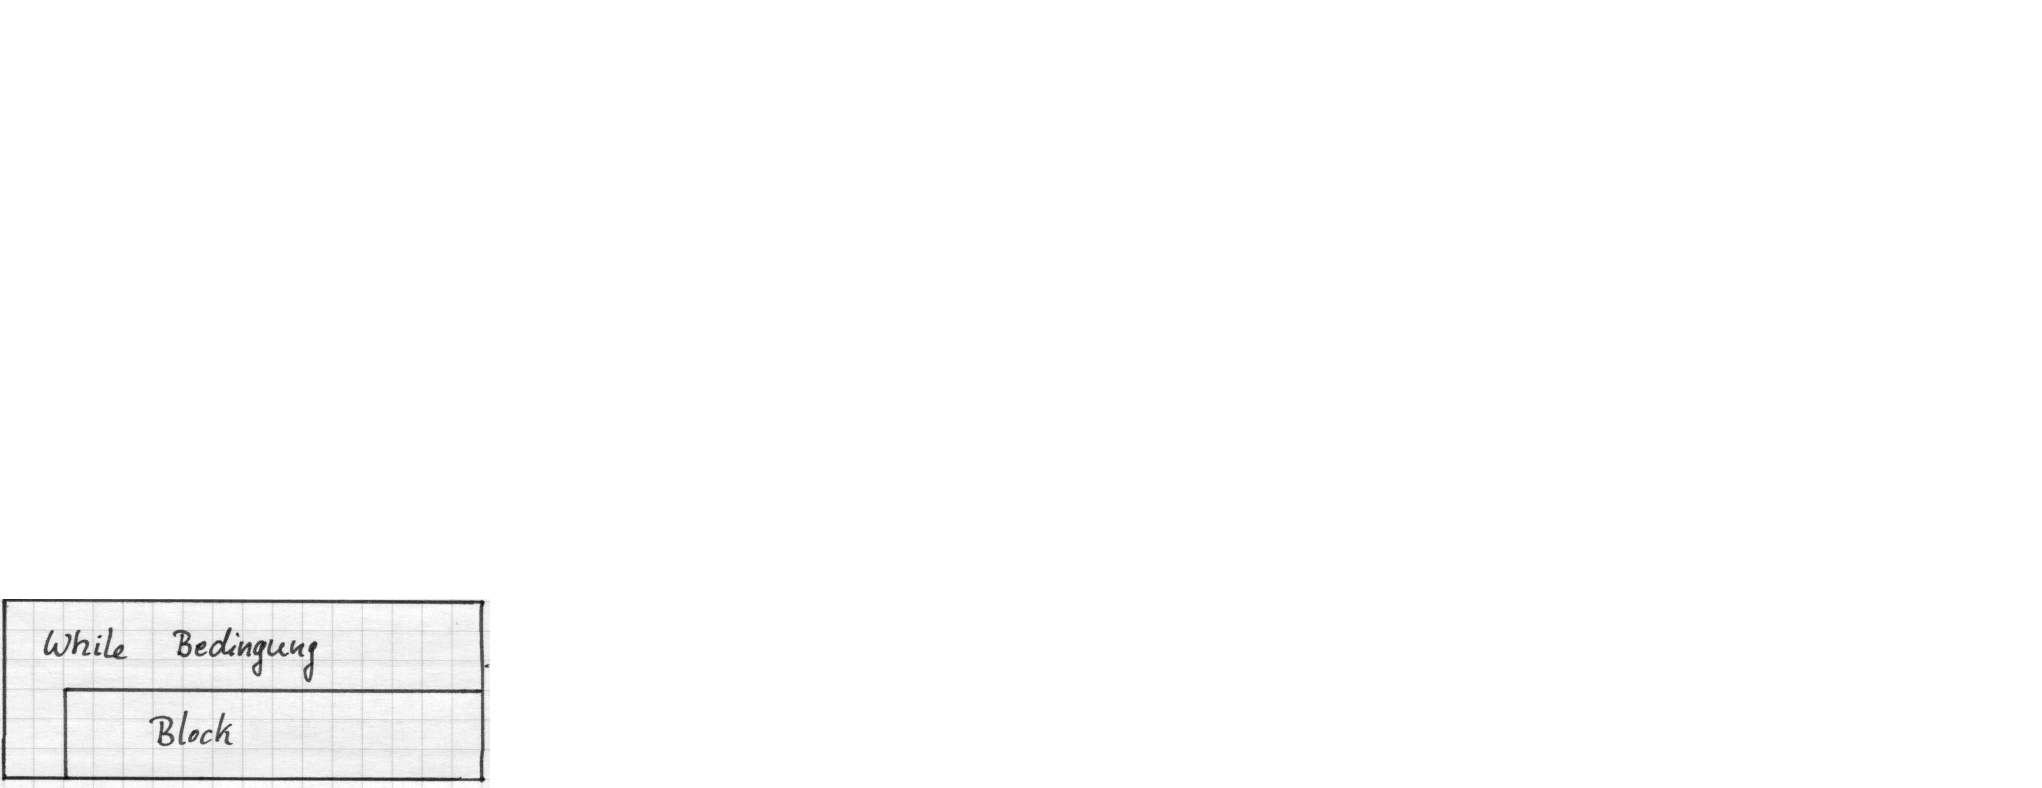
\includegraphics[scale=0.15]{GIF/p39.eps}
\end{minipage}

\textbf{Beispiel}: Bestimme den aufgerundeten Binärlogarithmus (Basis~2)
einer einzulesenden Zahl.\index{Bin\"arlogarithmus}
\includecode[linerange={7-11,13-22,25-26}]{Ex450.cpp}{Ganzzahliger Anteil des Binärlogarithmus einer Zahl}
%
% 
% \underline{Struktogramm}: %\\
% % \begin{latexonly}
% %   \special{psfile=GIF/p39.eps.gz
% % 	   hscale=15 vscale=15
% % 	   voffset=-55
% % 	  }
% %   \vspace{2cm}
% % \end{latexonly}
% % \begin{htmlonly} \\ \htmladdimg{p39_4.jpg}{}  \end{htmlonly}
% 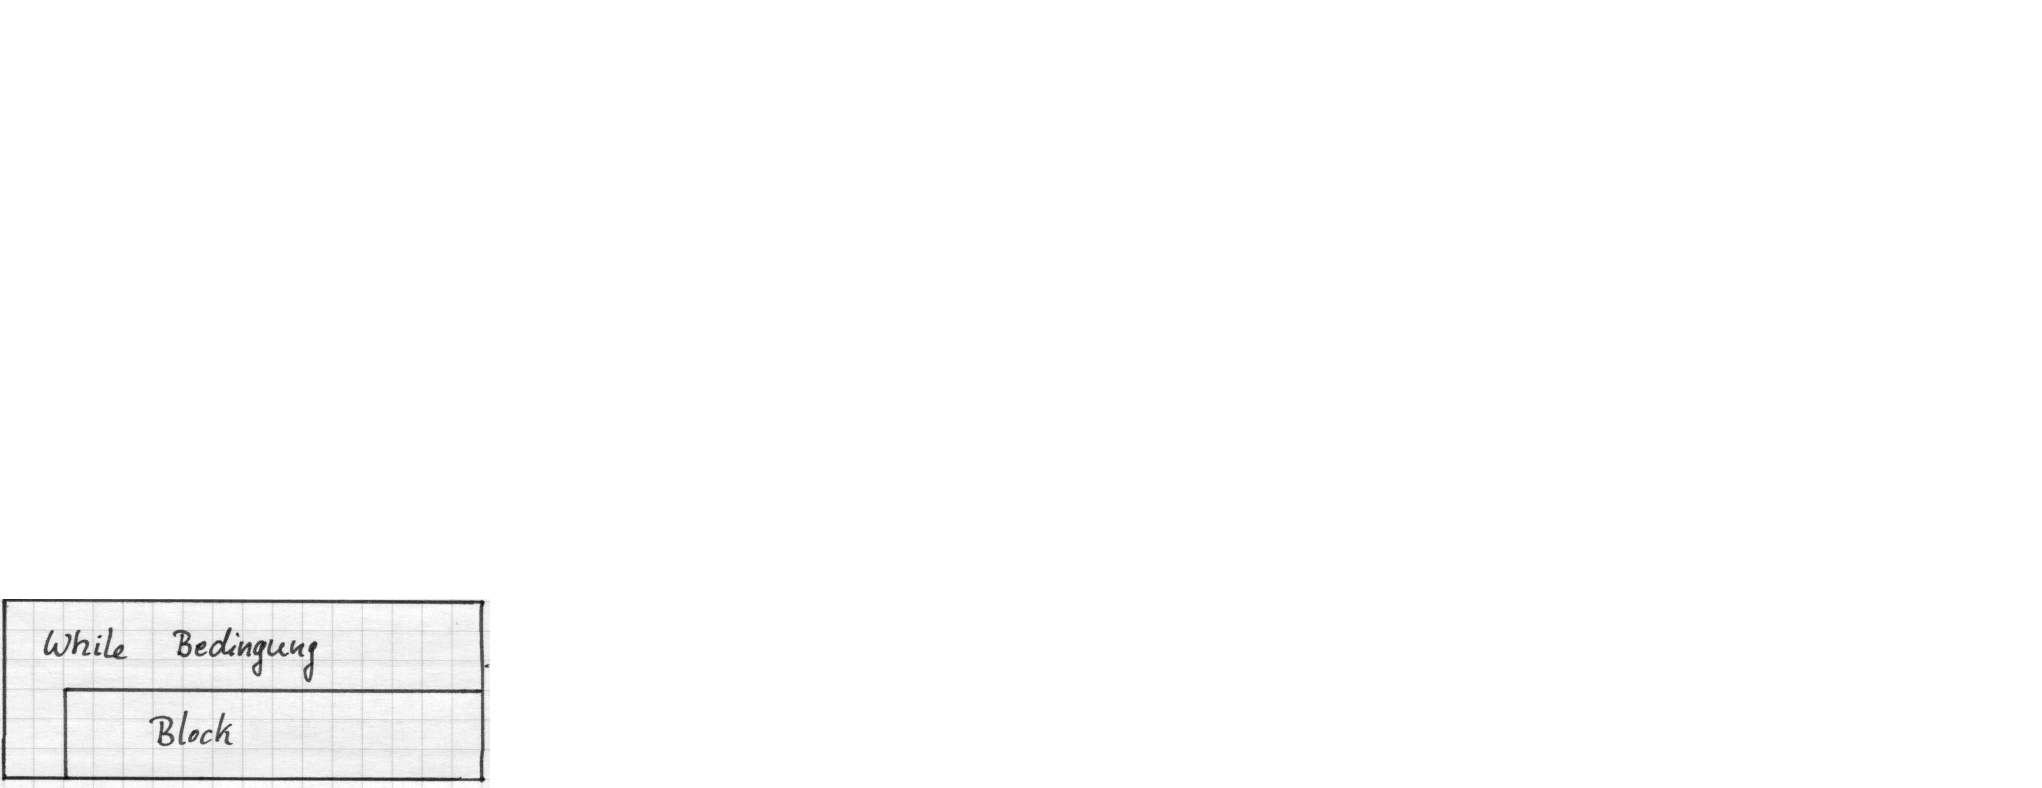
\includegraphics[scale=0.15]{GIF/p39.eps}


\underline{Bemerkung:} Falls der allererste Test im abweisenden Zyklus \texttt{false}
ergibt, dann wird der Anweisungsblock im Zyklusinneren
nie ausgef"uhrt (der Zyklus wird abgewiesen).

%
%
\section[Nichtabweisender Zyklus]{Nichtabweisender Zyklus (\texttt{do}-\texttt{while}-Schleife)}
\label{p:4.6}
%
Beim nichtabweisenden Zyklus steht die Anzahl der Durchl"aufe nicht
a-priori fest, der Abbruchtest erfolgt \textbf{nach} dem Durchlauf
eines Zyklus. Somit durchl"auft der nichtabweisende Zyklus mindestens
einmal die Anweisungen im Zyklusinneren.
\index{nichtabweisender Zyklus}\index{do-while-Schleife|see{nichtabweisender Zyklus}}
\index{nichtabweisender Zyklus!Abbruchtest}

% Die allgemeine Form ist
% 
% \mbox{}\hfill
% \begin{minipage}[t]{0.6\textwidth}
% \begin{verbatim}
% do
%   <anweisung>
% while (<logischer ausdruck>) ;
% \end{verbatim}
% \end{minipage}
% \hfill\mbox{}
% 
% \underline{Struktogramm}: \\
% % \begin{latexonly}
% %  \special{psfile=GIF/p40.eps.gz
% % 	  hscale=15 vscale=15
% % 	  voffset=-55
% % 	 }
% %  \vspace{2cm}
% % \end{latexonly}
% % \htmladdimg{p40_4.jpg}{}
% 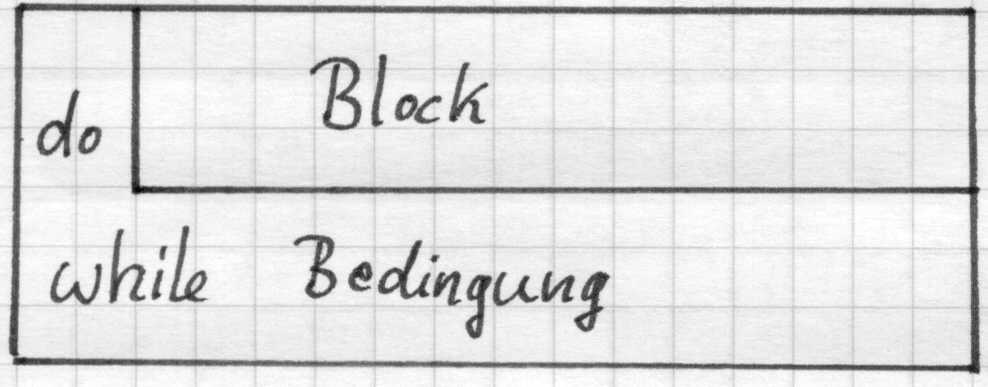
\includegraphics[scale=0.15]{GIF/p40.eps}

\begin{minipage}[t]{0.5\textwidth}
Die allgemeine Form ist\\[1ex]
\phantom{XXX}\verb|do| \\
\phantom{XXX}\verb|    <anweisung>|\\
\phantom{XXX}\verb|while (<logischer ausdruck>) ;|
\end{minipage}
\begin{minipage}[t]{0.4\textwidth}
\underline{Struktogramm}: %\\
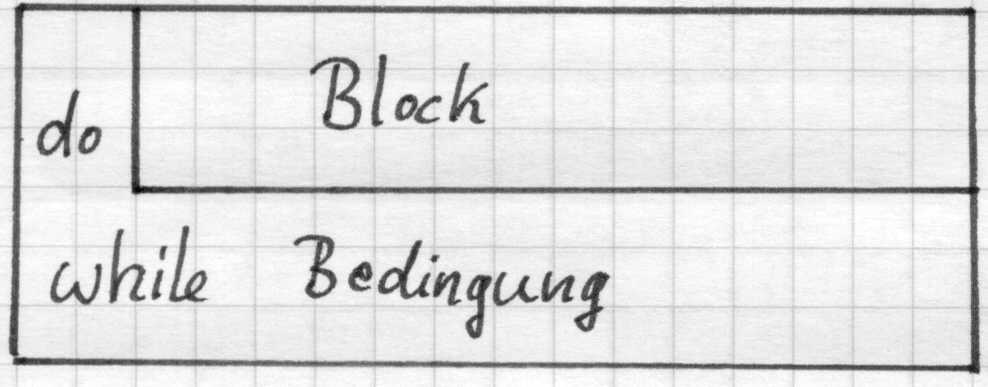
\includegraphics[scale=0.15]{GIF/p40.eps}
\end{minipage}



\textbf{Beispiel}: Es wird solange ein Zeichen von der
Tastatur eingelesen, bis ein \textit{x} eingegeben wird.
\includecode[linerange={7-19,22-23}]{Ex460.cpp}{Zeicheneingabe bis zum Exit-Zeichen \texttt{x}}
%

Betrachten wir ein etwas anspruchsvolleres \textbf{Beispiel}, und zwar soll
die L"osung von $\sin(x) = x/2$ mit $x\in(0,\pi)$ bestimmt werden.
Hierzu betrachtet man die "aquivalente Nullstellenaufgabe: Bestimme
die Nullstelle $x_0\in(0,\pi)$ der Funktion
$f(x) := \sin(x) - x/2 = 0$\enspace.\index{Nullstellen}
\label{bsp:bisection0}
\\
\underline{Analytisch:} Kein praktikabler L"osungsweg vorhanden.
\\
\underline{Graphisch:} Die Funktion $f(x)$ wir graphisch dargestellt
und das L"osungsintervall manuell verkleinert (halbiert).
Diesen Proze"s setzt man so lange fort, bis $x_0$ genau genug,
d.h., auf eine vorbestimmte Anzahl von Stellen genau,
bestimmt werden kann. \\[0.5ex]
% \epsfig{file=Ex46202.eps,height=4cm} \hfill
% 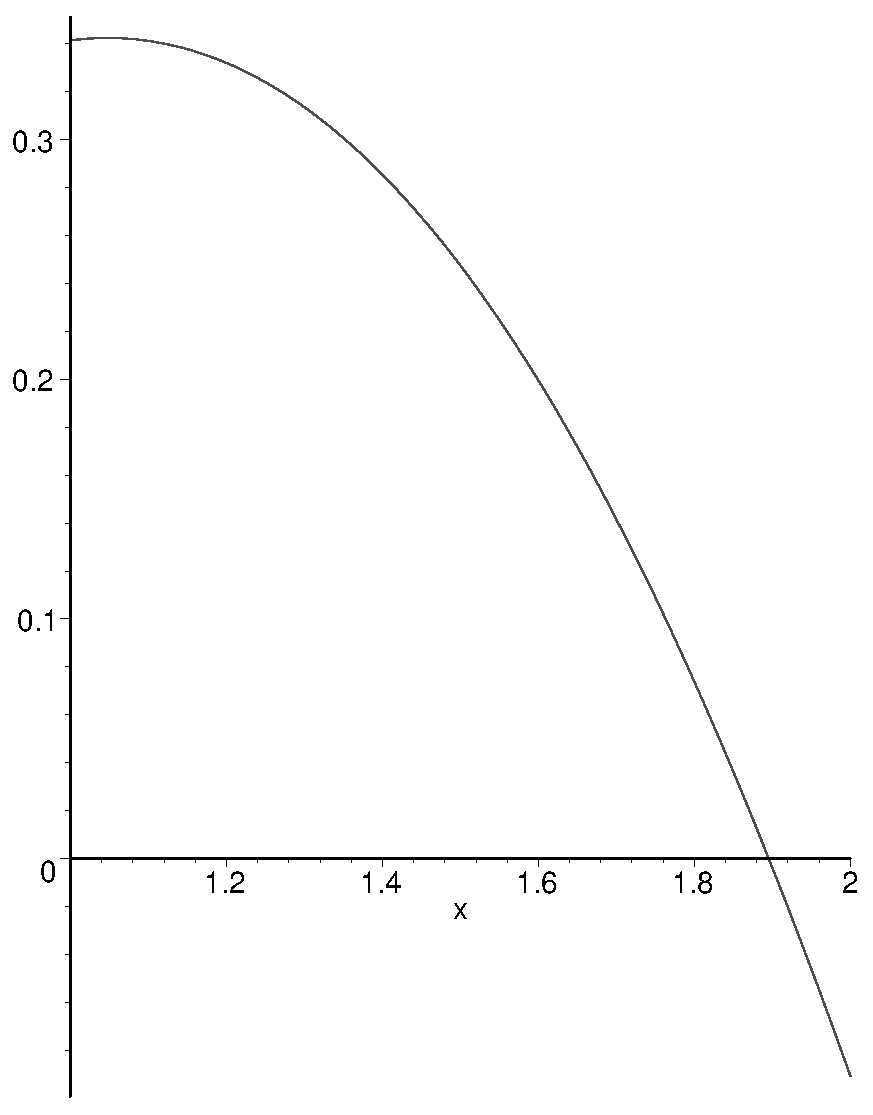
\epsfig{file=Ex46203.eps,height=4cm} \hfill
% 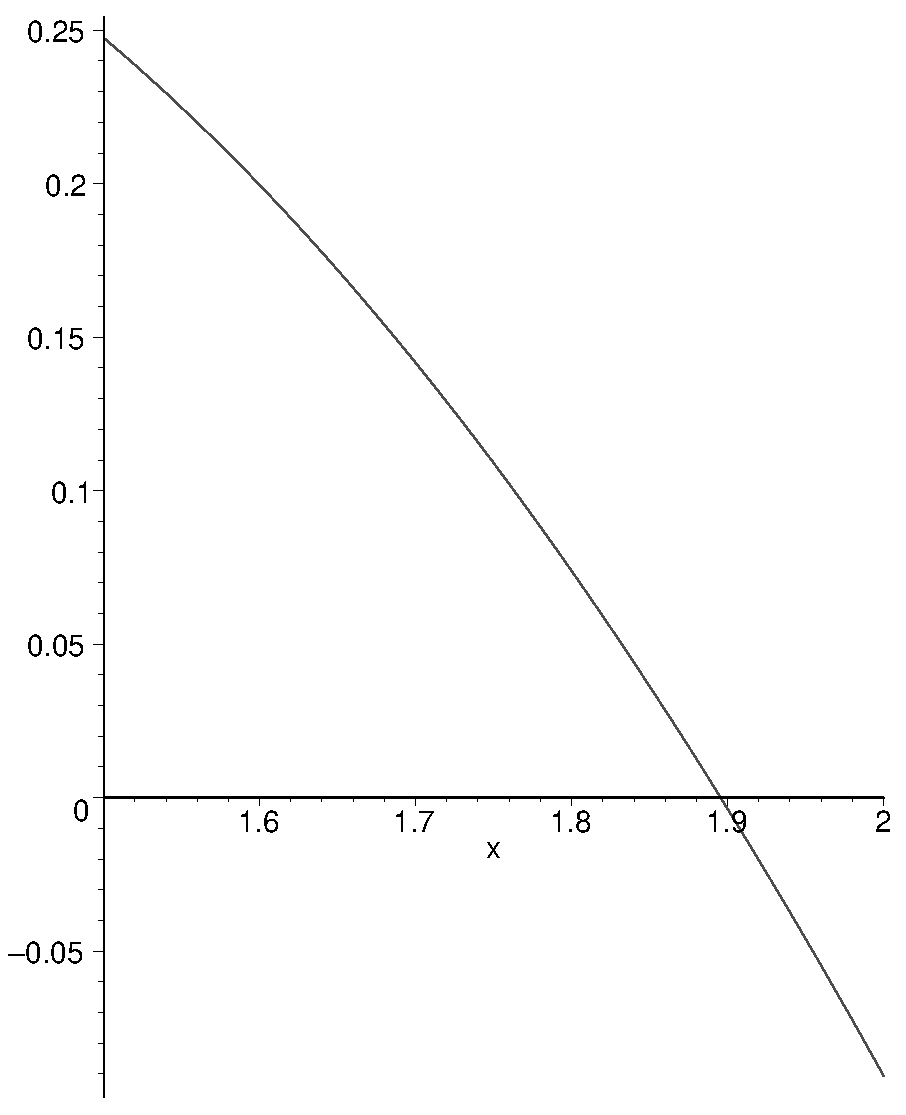
\epsfig{file=Ex46204.eps,height=4cm}
%
\includegraphics[height=4cm]{Ex46202.eps} \hfill
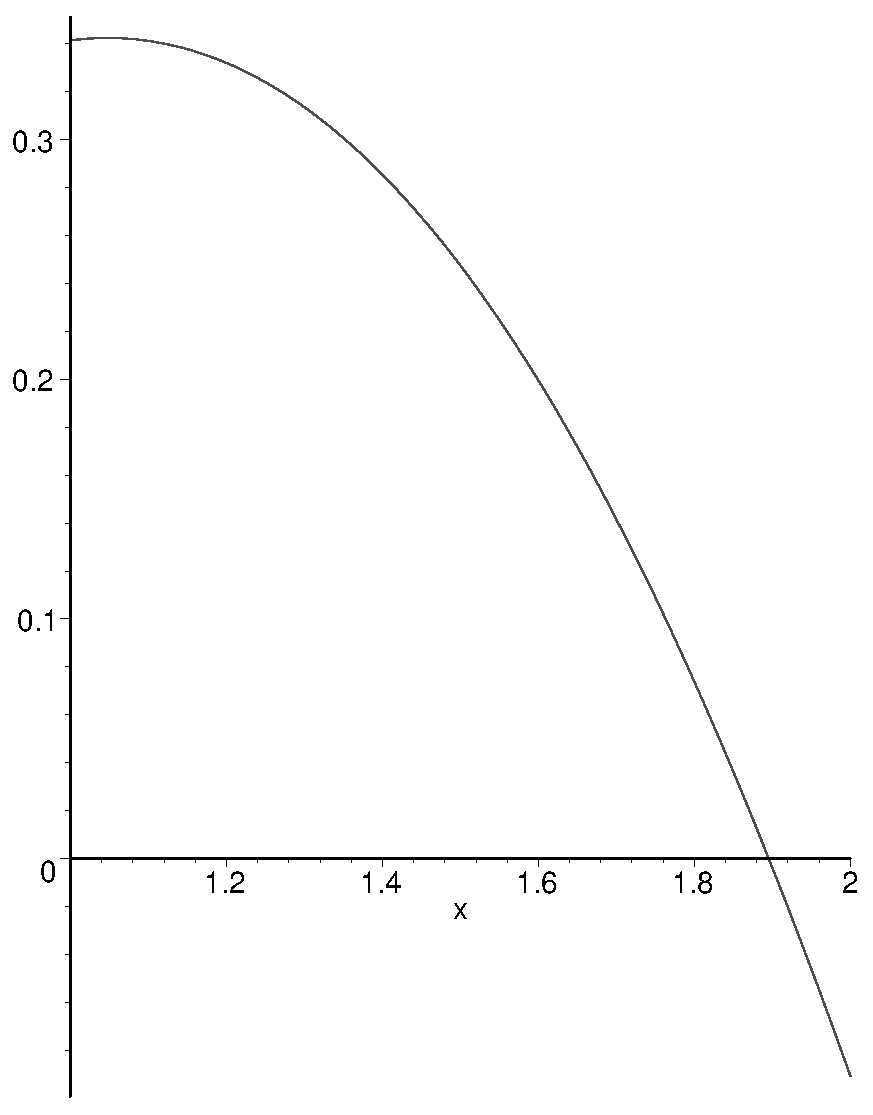
\includegraphics[height=4cm]{Ex46203.eps} \hfill
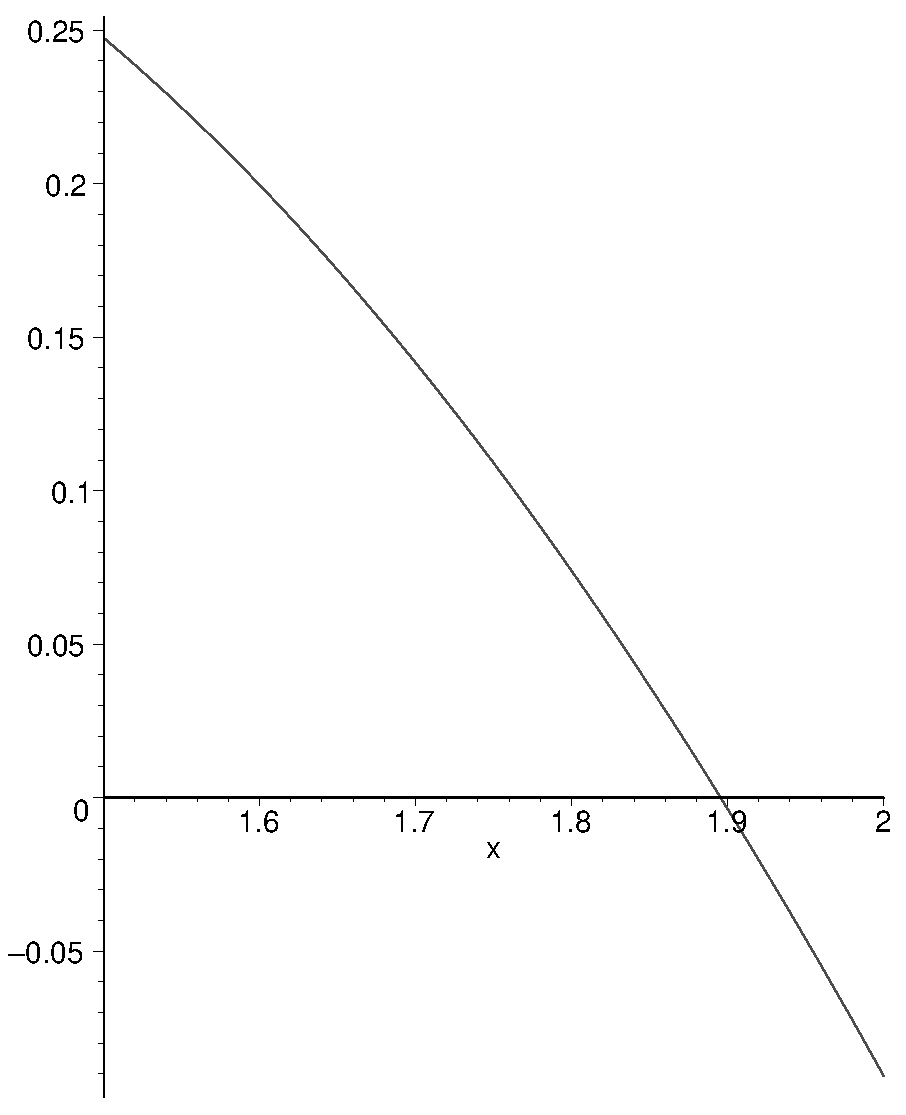
\includegraphics[height=4cm]{Ex46204.eps}
\\[0.5ex]
\underline{Numerisch:} Obiges, graphisches Verfahren kann auf ein
rein numerisches Verfahren im Computer "ubertragen werden
(der \textit{MAPLE}-Aufruf \texttt{fsolve(sin(x)=x/2,x=0.1..3}
liefert als N"aherungsergebnis $x_0 = 1.895494267$\enspace).
\bspfile{Ex462.mws}
Wir entwickeln ein Programm zur Bestimmung der Nullstelle
von $f(x) := \sin(x) - x/2$ im Intervall $[a,b]$
mittels Intervallhalbierung, wobei zur Vereinfachung
angenommen wird, da"s $f(a) >0$ und $f(b)<0$ ist.
Der Mittelpunkt des Intervalls sei mit $c:=(a+b)/2$ bezeichnet.
Dann k"onnen wir "uber die L"osung Folgendes aussagen:
$
\begin{cases}
 x_0 := c 	& \text{falls } f(c) = 0 \\
 x_0 \in [c,b]	& \text{falls } f(c) > 0 \\
 x_0 \in [a,c]	& \text{falls } f(c) < 0
\end{cases}
$\enspace.
%
Durch Redefinition der Intervallgrenzen $a$ und $b$ kann die
Nullstellensuche auf das kleinere (halbierte) Intervall
reduziert werden. Wir demonstrieren die Umsetzung mittels
eines nichtabweisenden Zyklus.
\bspfile{Ex462.cpp}

% 
% \underline{Struktogramm}: \\
% % \begin{latexonly}
% %   \special{psfile=GIF/p41a.eps.gz
% % 	   hscale=20 vscale=20
% % 	   voffset=-180
% % 	  }
% %   \vspace{6.3cm}
% % \end{latexonly}
% % \htmladdimg{p41a_4.jpg}{}
% 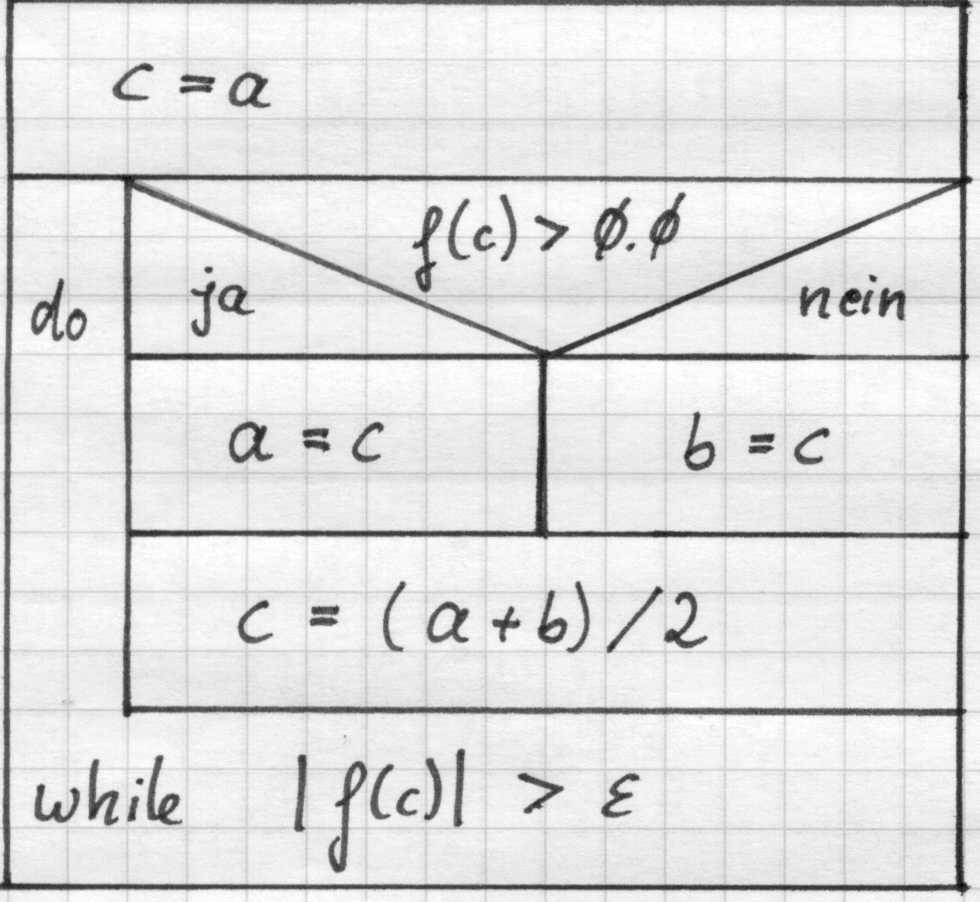
\includegraphics[scale=0.15]{GIF/p41a.eps}
% 
% 
% Obige Bisektion kann auch mittels eines
% abweisenden Zyklus realisiert werden.\index{Bisektion}
% \\
% % \begin{latexonly}
% %   \special{psfile=GIF/p41b.eps.gz
% % 	   hscale=20 vscale=20
% % 	   voffset=-180
% % 	  }
% %   \vspace{7cm}
% % \end{latexonly}
% % \htmladdimg{p41b_4.jpg}{}
% 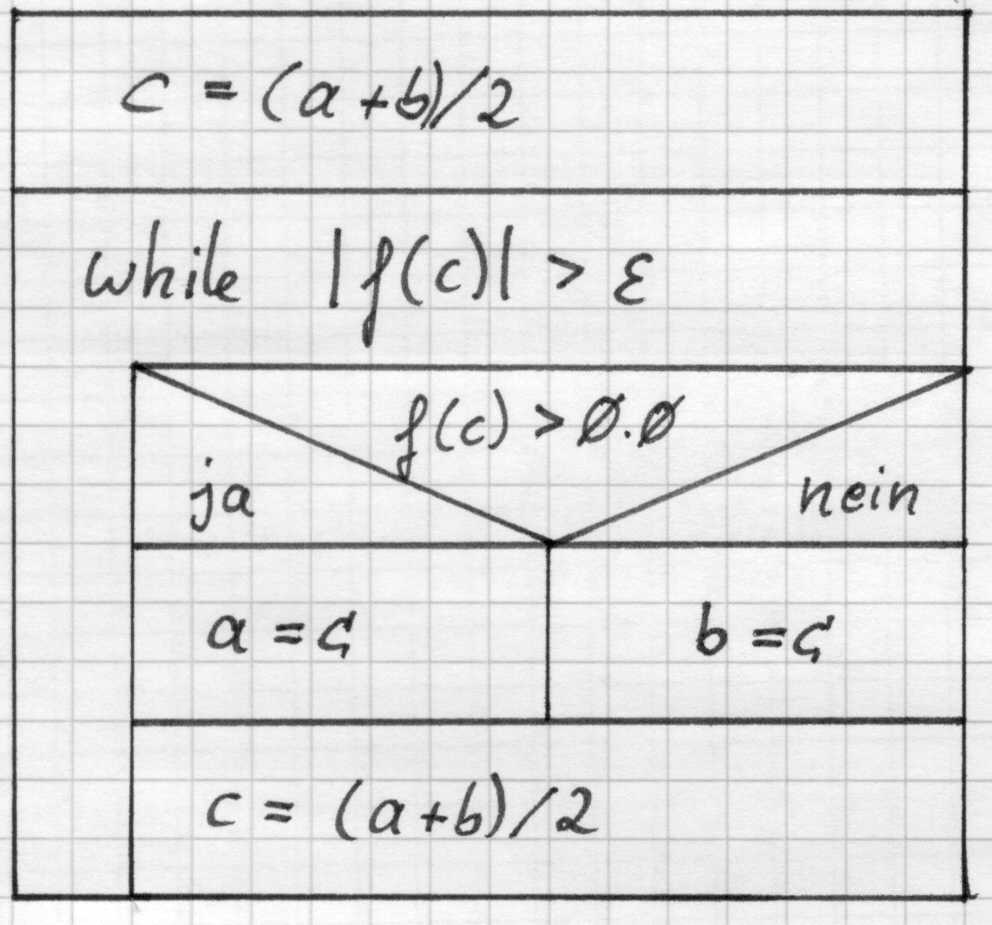
\includegraphics[scale=0.15]{GIF/p41b.eps}
%%%%%%%%%%%%%%%%%%%%%%%%%%%%%%%%%
\begin{minipage}{0.45\textwidth}
 \underline{nichtabweisender Zyklus}: \\
 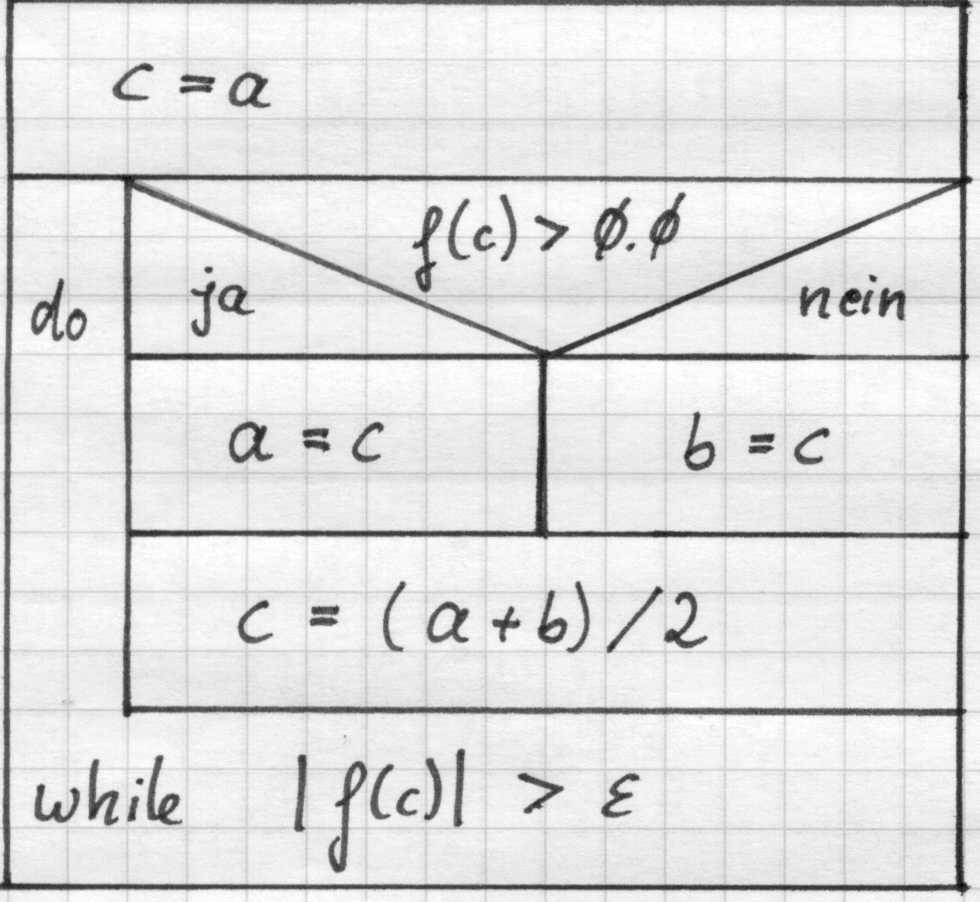
\includegraphics[scale=0.15]{GIF/p41a.eps}
\end{minipage}
\hfill
\begin{minipage}{0.45\textwidth}
 \underline{abweisender Zyklus}: \\
 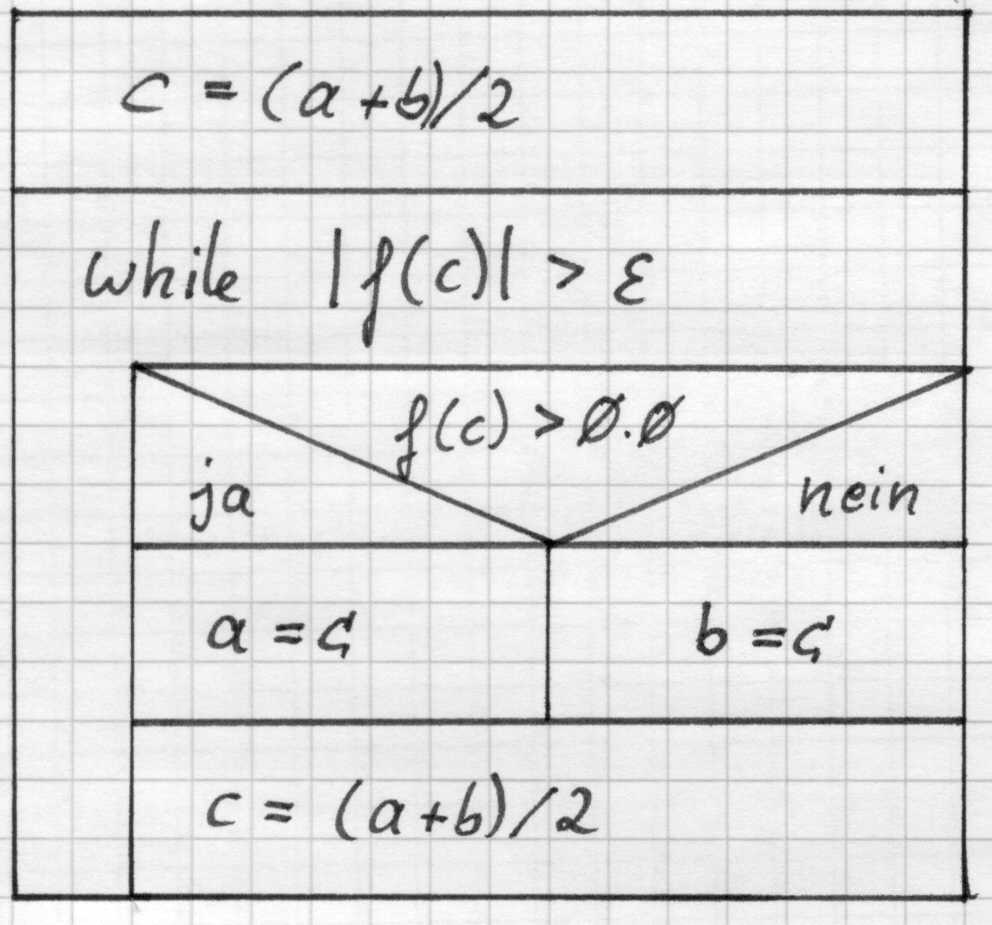
\includegraphics[scale=0.15]{GIF/p41b.eps}
\end{minipage}
\\
Wir realisieren obige Bisektion als nichtabweisenden Zyklus.\index{Bisektion}
%
\includecode[linerange={7-14,19-20,45-62,67-68}]{Ex462.cpp}{Bisektion als nichtabweisender Zyklus}
%

Da Gleitkommazahlen nur mit limitierter Genauigkeit\index{Gleitkommazahl!Genauigkeit}
arbeiten, resultiert
ein Abbruchtest $f(c) = 0$ meist in einem endlosen Programm.\index{Abbruchtest}
Dem ist ein Abbruchtest wie $|f(c)| < \varepsilon$ mit einer
vorgegebenen Genauigkeit $0< \varepsilon \ll 1$ vorzuziehen.

%\enlargethispage{1ex}
\underline{Bemerkung:}
Z"ahlzyklen (\verb|for|), welche \underline{mindestens einen} Zyklus
ausf"uhren, k"onnen sowohl durch abweisende (\verb|while|)
als auch durch nichtabweisende Zyklen (\verb|do while|)
"aquivalent ausgedr"uckt werden.
Diese "Aquivalenz kann bei Verwendung der Anweisungen in \S~\ref{p:4.8}
verloren gehen.
Falls in einem Z"ahlzyklus der Abbruchtest stets \texttt{false} ergibt, d.h.
der Schleifenk"orper wird nie ausgef"uhrt, dann ist
der entsprechende abweisende Zyklus nach wie vor "aquivalent. Jedoch
ist der nichtabweisende Zyklus nicht mehr "aquivalent, da der dortige
Schleifenk"orper auch in diesem Fall einmal abgearbeitet wird.
\bspfile{Loops.cpp}
%Siehe das Beispielfile~\textit{Loops.cpp}.
%
%
%
\section{Mehrwegauswahl (\texttt{switch}-Anweisung)}
\label{p:4.7}
%
Die Mehrwegauswahl erm"oglicht ein individuelles Reagieren
auf spezielle Werte einer Variablen.
\index{Mehrwegauswahl}\index{switch!Mehrwegauswahl}

\mbox{}\hfill
\begin{minipage}[t]{0.6\textwidth}
\begin{verbatim}
switch (<ausdruck>)
 {
   case <konst_ausdruck_1> :
        <anweisung_1>
	[break;]
   ...
   case <konst_ausdruck_n> :
        <anweisung_n>
	[break;]
   default:
        <anweisung_default>
 }
\end{verbatim}
\end{minipage}
\hfill\mbox{}

\textbf{Beispiel}: Ausgabe der Zahlw"orter f"ur die ganzzahlige Eingaben
	$\{1,2,3\}$.
	%dem Intervall~$[1,3]$.
%\includecode[linerange={7-14,19-20,45-62,67-68}]{Ex470.cpp}{Demonstration der Switch-Anweisung}
\includecode[firstline=5]{Ex470.cpp}{Demonstration der Switch-Anweisung}
%

Obige \verb|switch|-Anweisung k"onnte auch mit einer
Mehrfachverzweigung (Seite~\pageref{mehrweg}) implementiert werden,
jedoch werden in der \verb|switch|-Anweisung die einzelnen Zweige
explizit "uber die  \verb|break;|-Anweisung verlassen.
Ohne \verb| break; | wird zus"atzlich der zum nachfolgenden Zweig
geh"orige Block abgearbeitet.

Es ist in C++ \emph{nicht} m"oglich, \emph{Bereiche} anzugeben, etwa der Art
\texttt{case 7..11: Anweisung; break;} anstelle der korrekten
C++-Vorgangsweise~\cite[\S1.8.4]{Breymann:2017:DCP}
% \begin{verbatim}
\\[0.5ex]
\verb| case 7: case 8: case 9: case 10: case 11:| \\
\verb|    Anweisung;| \\
\verb|    break;|
% \end{verbatim}
%
%
%
\section[Unbedingte Steuerungs"ubergabe]{Anweisungen zur unbedingten Steuerungs"ubergabe}
\label{p:4.8}
%
%\begin{itemize}
\begin{description}
 \item[\texttt{break}] Es erfolgt der sofortige Abbruch
	 der n"achst"au{\ss}eren
	 \verb|switch|, \verb|while|, \verb|do-while|, \verb|for|
	 Anweisung.\index{break}
 \item[\texttt{continue}] Abbruch des aktuellen und Start des
 	n"achsten Zyklus einer \verb|while|, \verb|do-while|, \verb|for|
	Schleife.
	\bspfile{Ex480.cpp}
 \item[\texttt{goto <marke>}] Fortsetzung des Programmes an der mit
 	\\
	\verb|<marke> : <anweisung>|
	\\
	markierten Stelle.
\end{description}
%\end{itemize}

\underline{Bemerkung :} Bis auf \verb|break| in
der \verb|switch|-Anweisung sollten obige Anweisungen
sehr sparsam (besser gar nicht) verwendet werden, da
sie dem strukturierten Programmieren zuwiderlaufen und
im Extremfall einen gef"urchteteten Spaghetticode erzeugen.
Wenn man das strukturierte Programmieren gut beherrscht, dann kann die
gezielte Verwendung von \verb|break| und \verb|continue| zu schnellerem Code
f"uhren.

\textbf{Obige Anweisungen aus \S\ref{p:4.8} sind
im Rahmen dieser LV zur L"osung von "Ubungsaufgaben und im Test nicht erlaubt.}
Einzige Ausnahme ist \verb|break| in der \verb|switch|-Anweisung.































\chapter{Strukturierte Datentypen}
\label{p:5}
%
%
Wir werden in diesem Kapitel neue M"oglichkeiten der Datenspeicherung
einf"uhren.
\begin{itemize}
  \item \textbf{Feld (array)}, \textbf{Liste}: \\
  	Zusammenfassung von  Elementen gleichen Typs.
	\index{Feld}\index{array|see{Feld}}
  \item \textbf{Struktur (struct)}: \\
  	Zusammenfassung von Komponenten verschiedenen Typs.
	\index{Struktur}\index{struct|see{Struktur}}
  \item \textbf{Union (union)}: \\
  	"Uberlagerung mehrerer Komponenten verschiedenen Typs auf
	dem gleichen Speicherplatz.
	\index{union}
  \item \textbf{Aufz"ahlungstyp (enum)} \\
  	Grunddatentyp mit frei w"ahlbarem Wertebereich.
	\index{Aufz\"ahlungstyp}\index{enum|see{Aufz\"ahlungstyp}}
\end{itemize}
%
Eine dar"uber hinausgehende, sehr gute Einf"uhrung in Algorithmen und Datenstrukturen
ist in~\cite{PombergerDobler:2008:AUD} zu finden.
%
\section{Felder}
\label{p:5.1}
%
In einem Feld/Array werden Daten (Elemente) gleichen Typs zusammengefa"st.
Die klassischeVereinbarung eines statischen Feldes ist in C (geht auch in C++)
\index{Feld!eindimensional}\index{Feld!statisch|(}
\centerline{\texttt{ <typ> <bezeichner>[dimension];}}
%
wobei die eckigen Klammern ``['' und ``]''
unabdingbarer Bestandteil der Vereinbarung  sind.
Ein eindimensionales Feld entspricht mathematisch einem Vektor.
Hierbei wird zwischen \emph{statisch}en Feldern (Länge des Feldes ist zur Compilezeit bekannt)
und \emph{dynamisch}en Feldern (Feldlänge kann erst aus Daten des Programmes bestimmt werden bzw.\  ändert sich
während des Programmablaufes) unterschieden.
\index{Vektor}
%
\includecode[linerange={9-17,25-25,37-37}]{Ex510.cpp}{Statisches C-Array}

Die eckigen Klammern dienen im Vereinbarungsteil der Dimensionsvereinbarung
\verb|x[N]| und  im Anweisungsteil dem Zugriff auf einzelne
Feldelemente \verb|x[3]|\enspace.
Das Feld kann schon bei Deklaration initialisiert werden:
\index{Feld!Dimension}\index{Feld!Deklaration}\index{Feld!Initialisierung}
\\
\verb|double x[N] = {9,7,6,5,7}|

\underline{Achtung :} Die Numerierung der Feldelemente
beginnt mit 0. Daher darf nur auf Feldelemente
$x_i$, $i=0,\ldots,N-1$ zugegriffen werden.\index{Feld!Numerierung}\index{Feld!Feldelemente}
Andernfalls sind mysteri"oses Programmverhalten,
unerkl"arliche Fehlberechnungen und pl"otzliche Programmabst"urze
zu erwarten, deren Ursache nicht offensichtlich ist da
sie eventuell erst in weit entfernten Programmteilen auftreten k"onnen.
Diese Fehler müssen dann mit \emph{Memory-Checkern} mühsam gesucht werden. 
Ein gutes und freies Programm hierfür ist \texttt{valgrind} unter Linux/Unix bzw.\
der \emph{inspector} enthalten in der Intel Toolbox (freie Studentenversion).

Wir werden im Weiteren \textbf{nicht die C-Arrays benutzen, sondern die nachfolgenden C++-Vektoren}.
Deren Deklaration ist unterschiedlich von oberer Deklaration, der Zugriff kann identisch erfolgen
und die C++-Vektoren haben mehr Funktionalität.
%
%
\subsection{Dynamischer C++-Vektor}
\label{p:5.1.1}
%
Wir illustrieren den C++-Vektor
\ghref{http://www.cplusplus.com/reference/vector/vector/}{\texttt{vector <T>}}
 mit dem Beispiel der Berechnung der $L_{2}$-Norm eines Vektors, d.h.,
$\parallel \underline{x} \parallel_{L_2} :=
 \sqrt{\sum\limits_{i=0}^{N-1} x_i^2}
$\enspace.
%
%
%\includecode[linerange={7-8,11-23,30-30}]{bsp511a.cpp}{Berechnung der $L_{2}$-Norm eines Vektors}
\includecode[firstline=5]{bsp511a.cpp}{Berechnung der $L_{2}$-Norm eines Vektors}
%
Ein paar Bemerkungen zu Listing~\ref{lst:bsp511a.cpp}:
\begin{itemize}
	\item Zeile 10: Diese Deklaration einer Variablen vom Typ \verb|vector<double>| enthält die
	Anzahl der Elemente, welche zur Compilezeit nicht feststand.
	\item Die Länge von Vektor \verb|x| läßt sich mit \verb|x.resize(n+4)| im Programmablauf ändern
	(auch auf einen kürzeren Vektor).
	\item Zeile 11: Die Länge des Vektors kann über die Methode \verb|x.size()| abgefragt werden, d.h.,
	diese Information ist Teil des C++-Vektors.
	\item Zeile 16: Der Zugriff auf Element~$k$ erfolgt über \verb|x[k]| am schnellsten.
	 Ein unzulässiger Zugriff \verb|x[n]| ($n \not\in [0,x.size()]$) wird jedoch nicht vom Programm abgefangen
	 und führt zum Programmabbruch oder (schlimmer) zu nicht nachvollziehbarem Verhalten des Programmes.
	 \item Zeile 12: C++-Vektoren erlauben den gesicherten Zugriff auf Vektorelemente über
	 \verb|x.at(k)|. Im Falle von $k \not\in [0,x.size()]$ bricht das Programm mit einer Fehlermeldung ab.
\end{itemize}
Mit obigem Code haben wir die dynamischen Möglichkeiten von \texttt{vector} noch nicht voll ausgeschöpft.
Dazu betrachten wir die gleiche Berechnung wie oben, werden aber die Anzahl der Komponenten
an hand der einzugebenden Daten bestimmen.
%
\pagebreak[2]
%\includecode[linerange={7-8,11-23,30-30}]{bsp511b.cpp}{Mehr Dynamik beim Vektor}
\includecode[firstline=5]{bsp511b.cpp}{Mehr Dynamik beim Vektor}
%
In Listing~\ref{lst:bsp511b.cpp} sind ein paar interessante Details untergebracht:
\begin{itemize}
	\item Zeile 7: Der Vektor hat die Länge 0.
	\item Zeilen 8-13: Es werden solange Daten eingegeben, bis die Eingabegröße $<0$ ist. Dabei wächst der Vektor
	in jedem Durchlauf um ein Element.
	\begin{itemize}
	  \item Zeile 11: Die Methode \ghref{http://www.cplusplus.com/reference/vector/vector/push_back/}{\texttt{push\_back}}
	  fügt den übergebenen Wert \texttt{tmp} als neues letztes Element an den Vektor an.
	  \item Zeile 12: Die Methode \texttt{back} greift auf das aktuelle, letzte Element des Vektors zu (und testet, ob
	  dieses nichtnegativ ist).
	  \item Zeile 13:  Die Methode \texttt{pop\_back} entfernt das negative letzte Element und verkürzt den Vektor
	  entsprechend.
	\end{itemize}
	\item Zeile 15: Die Methode \texttt{size} liefert die Vektorlänge normalerweise als \verb|unsigned int|
	zurück (kann aber auch anders definiert sein!).
	Wenn die Loopvariable~\texttt{k} nun als \verb|int| deklariert ist, werden beim Vergleich \verb|k<x.size()|
	unterschiedliche Datentypen verglichen. Dies ist im Normalfall kein Problem, führt aber zu lästigen
	Compilerwarnungen. Exakterweise nimmt man daher \verb|size_t| als Datentyp der Loopvariablen.
\end{itemize}
%
%
\subsection{Statischer C++-Vektor}
\label{p:5.1.2}
Natürlich kann man den dynamischen Vektor~\texttt{vector<T>} auch als statischen Vektor benutzen.
Dies ist am Anfang auch die einfachste Lösung.

Um aber die volle konzeptionelle Kompatibilität zum klassischen C-Vektor herzustellen, 
wurde mit dem C++11-Standard der statische Vektor
\ghref{http://www.cplusplus.com/reference/array/array/}{\texttt{array<T,N>}}
eingeführt bei welchem zur Compilezeit nicht nur der Datentyp~\texttt{T} sondern auch
die Länge~\texttt{N} festgelegt sind. Dynamische Methoden sind für diesen Vektor nicht verfügbar.
%
\includecode[firstline=5]{bsp511c.cpp}{Berechnung der $L_{2}$-Norm eines statischen C++-Vektors}
%
Im Listing~\ref{lst:bsp511c.cpp} hätte man in Zeile~7 genauso einen dynamischen Vektor nehmen können
(\verb|vector<double> x(10)|), bis auf das zu inkludierende Headerfile bliebe der restliche Code unverändert.


\subsection{Beispiele zu C++-Vektoren}
\label{p:5.1.3}
%
Als kleines \textbf{Beispiel} diene uns die Fibonacci Zahlenfolge,
welche "uber die zweistufige Rekursion\index{Fibonacci}
$$
f(n) _:= f(n-1) + f(n-2) \qquad n=2,\ldots
$$
mit den Anfangsbedingungen $f(0) = 0$, $f(1) = 1$ definiert ist.
%\exfile{Fibo1.cpp}
Zur Kontrolle k"onnen wir die
\ghref{http://de.wikipedia.org/wiki/Fibonacci-Folge\#Formel_von_Moivre-Binet}{Formel von Binet bzw.\  de Moivre}
%\htmladdnormallinkfoot{Formel von Binet bzw.\  de Moivre}
%{http://www.ee.surrey.ac.uk/Personal/R.Knott/Fibonacci/fibFormula.hpptml}
verwenden.
$$
f(n) = \frac{1}{\sqrt{5}}
 \left( \left(\frac{1+\sqrt{5}}{2}\right)^n
      - \left(\frac{1-\sqrt{5}}{2}\right)^n
 \right)
$$
%
\includecode[linerange={6-18,35-36}]{bsp_Fibo1.cpp}{Fibonacci numbers}
%

% \pagebreak[4]
\newpage
Als weiteres \textbf{Beispiel} sollen Minimum und Maximum eines
Vektors bestimmt und die entsprechenden Vektorelemente
miteinander vertauscht werden (analog zu Pivotisierung).
%\exfile{Ex513.cpp}
Dies beinhaltet die beiden Teilaufgaben: \\[1ex]
%
%
%%%%%%%%%%%%%%%%%%%%%%%%%%%%%%%%%%%%%%
% \begin{enumerate}
% \renewcommand {\labelenumi}{\alph{enumi})}
%  \item Bestimme Minimum und Maximum (und markiere die Positionen).
% \\
% %
% \underline{Struktogramm}: \\
% %\begin{latexonly}
% %  \special{psfile=GIF/p49a.eps.gz
% %	   hscale=65 vscale=65
% %	   voffset=-340
% %	}
% %  \vspace{11.9cm}
% %\end{latexonly}
% %\htmladdimg{p49a_4.jpg}{}
% 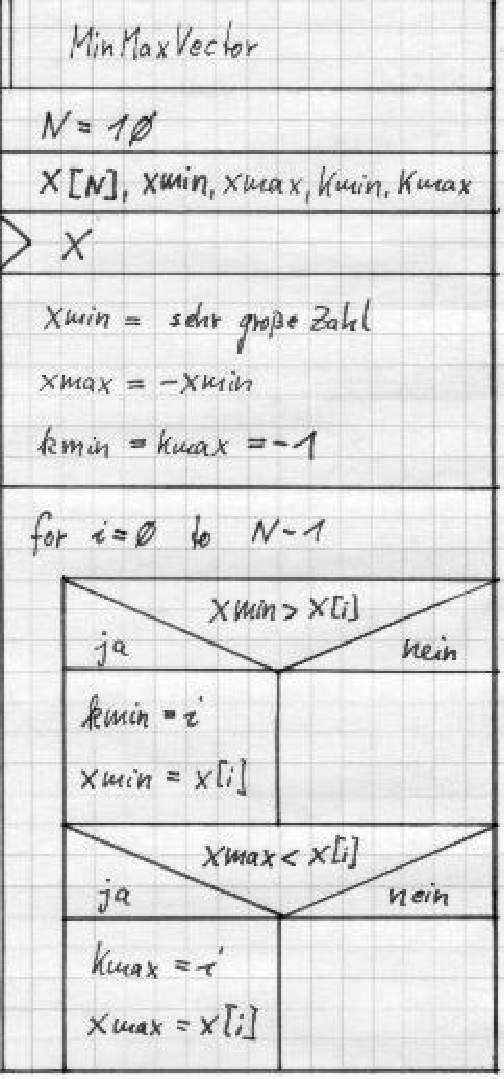
\includegraphics[scale=0.7]{GIF/p49a}
% 
% %
%  \item Vertausche Min/Max-Eintr"age. Bei Vektorl"ange~$0$ oder
%  	bei identischen Vektorelementen ist kein Vertauschen notwendig.
% \\
% %
% \underline{Struktogramm}: \\
% %begin{latexonly}
% %\begin{minipage}{0.4\textwidth}
% %\special{psfile=GIF/p49b.eps.gz
% %	 hscale=65 vscale=65
% %	 voffset=-130
% %	}
% %\mbox{}\\[4cm]
% %%\vspace{5.5cm}
% %\end{minipage}
% %\end{latexonly}
% %\htmladdimg{p49b_4.jpg}
% 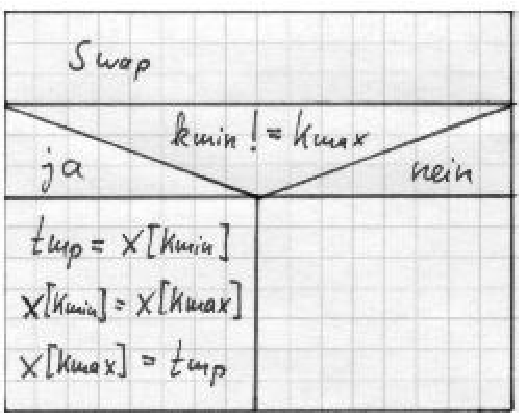
\includegraphics[scale=0.7]{GIF/p49b}
% %
% \hfill
% \begin{minipage}[b]{0.35\textwidth}
% Beim Vertauschen f"uhrt \\
% die naheliegende, erste Idee
% \verb| x[kmin] = x[kmax]| \\
% \verb| x[kmax] = x[kmin]| \\
% nicht zum Erfolg. Warum?
% \end{minipage}
% %
% \end{enumerate}
%%%%%%%%%%%%%%%%%%%%%%%%%%%%%%%%%%%%%%
\begin{minipage}[t]{0.45\textwidth}
  a) Bestimme Minimum und Maximum \\(und markiere die Positionen). \\[1ex]
%
 \underline{Struktogramm}: \\
 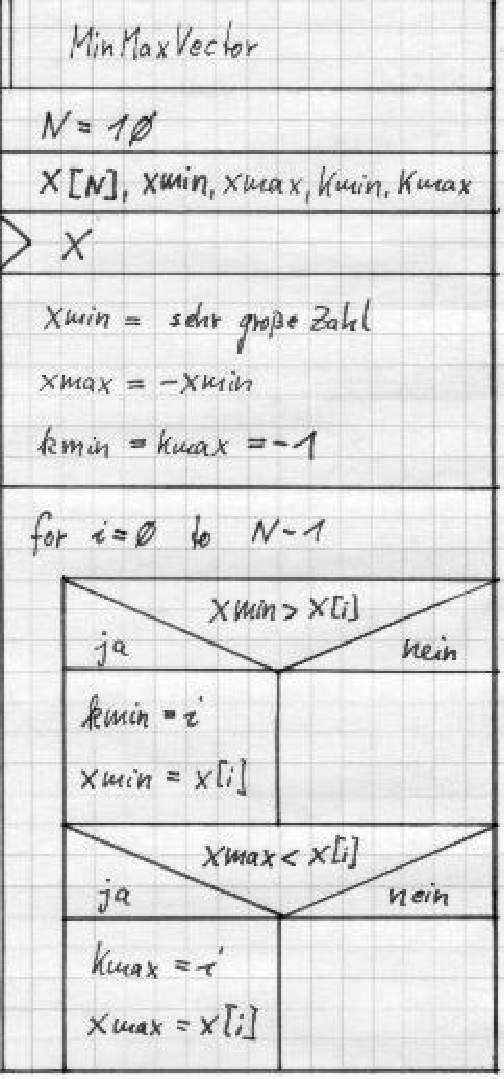
\includegraphics[scale=0.58]{GIF/p49a}
\end{minipage}
\hfill
\begin{minipage}[t]{0.45\textwidth}
 b) Vertausche Min/Max-Eintr"age. \\ Bei Vektorl"ange~$0$ oder
 	bei identischen Vektorelementen ist kein Vertauschen notwendig.
 	\\[1ex]
 %
\underline{Struktogramm}: \\
 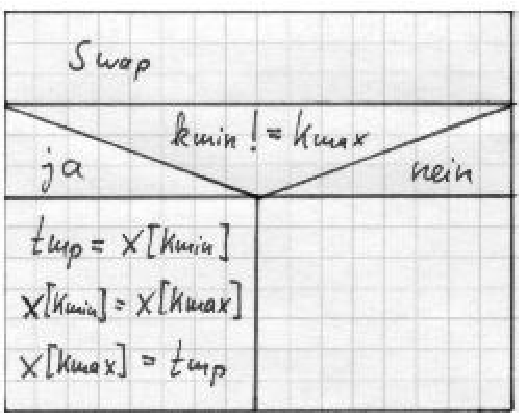
\includegraphics[scale=0.7]{GIF/p49b}
 \\[1ex]
 Beim Vertauschen f"uhrt \\
 die naheliegende, erste Idee
 \verb| x[kmin] = x[kmax]| \\
 \verb| x[kmax] = x[kmin]| \\
 nicht zum Erfolg. Warum?
\end{minipage}
%%%%%%%%%%%%%%%%%%%%%%%%%%%%%%%%%%%%%%
%
%
\includecode[linerange={7-16,27-49,60-61}]{bsp513.cpp}{Bestimme Min/Max eines Vektor und vertausche die Komponenten}
%
\index{numeric\_limits!max}\index{numeric\_limits}
In obigen beiden Listing wurden keine dynamischen Eigenschaften des Vektors benutzt,
daher hätten wir auch \verb|array<T,N>| verwenden können.
%
%
\subsection{Mehrdimensionale Felder in C++}
\label{p:5.1.4}
%
\subsubsection{Statische Matrizen}
\label{p:5.1.4.a}
%
%
Die Elemente der bisher betrachteten 1D-Felder sind im
Speicher hintereinander gespeichert (Modell des linearen Speichers), z.B,
wird der Zeilenvektor
\index{Feld!mehrdimensional}
\\[0.5ex]
\centerline{$\begin{pmatrix} x_0 & x_1 & x_2 & x_3 & x_4 \end{pmatrix}$}
\\
als
\\
%
\mbox{} \hfill\verb|double x[5];| \hfill\mbox{}
%
\\
vereinbart und gespeichert als
\\
%\centerline{\input{kap512a.pstex_t}}
\centerline{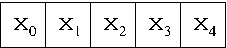
\includegraphics[scale=0.9]{kap512a.pdf}}
\\
wobei jede Zelle 8~Byte lang ist.

Ein zweidimensionales (statisches) Feld, z.B., eine Matrix~$A$ mit $N=4$~Zeilen
und $M=3$~Spalten
\index{Matrix}
\\[0.5ex]
\centerline{
$
A_{N \times M} :=
\begin{pmatrix}
 A_{00} & A_{01} & A_{02} \\
 A_{10} & A_{11} & A_{12} \\
 A_{20} & A_{21} & A_{22} \\
 A_{30} & A_{31} & A_{32}
\end{pmatrix}
$
}
\\[0.5ex]
kann im Speicher ebenfalls nur linear gespeichert werden, d.h.,
\\
% \centerline{\input{kap512b.pstex_t}}
\centerline{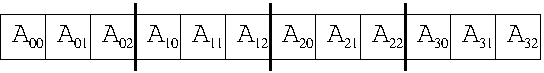
\includegraphics[scale=0.9]{kap512b.pdf}}
\\[0.5ex]
Daraus ergeben sich zwei M"oglichkeiten der 2D-Feldvereinbarung:
\begin{itemize}
 \item \underline{Variante 1 :} Als 2D-Feld.
%
\\[0.5ex]
\begin{minipage} {0.8\textwidth}
\begin{verbatim}
double A[N][M];               // Declaration in C
array<array<double,M>,N> A;   // Declaration in C++ (statisch)
A[3][1] = 5.0;                // Initialize A(3,1)
\end{verbatim}
\end{minipage}
%
 \item \underline{Variante 2 :} Als 1D-Feld.
 \label{page:2DarrayVariant2}
%
\\[0.5ex]
\begin{minipage} {0.8\textwidth}
\begin{verbatim}
double A[N*M];                // Declaration in C
array<double,M*N> A;          // Declaration in C++ (statisch)
A[3*M+1] = 5.0;               // Initialize A(3,1)
\end{verbatim}
\end{minipage}
%
\end{itemize}
%
\textbf{Beispiel}:  Als Beispiel betrachten wir die Multiplikation
der Matrix $A_{N \times M}$
bestehend aus $N=4$~Zeilen und $M=3$~Spalten
mit einem Zeilenvektor~$\underline{u}_M$
der L"ange~$M$.
Das Ergebnis ist ein Zeilenvektor~$\underline{f}_N$ der L"ange~$N$,
d.h., $\underline{f}_N : = A_{N \times M} \cdot \underline{u}_M$\enspace.
%
Die Komponenten von $\underline{f} = [f_0,f_1,\ldots,f_{N-1}]^T$
berechnen sich zu
%\bspfile{bsp514.cpp}
\begin{displaymath}
 f_i := \sum_{j=0}^{M-1} A_{i,j} \cdot u_j
 \qquad \forall i=0,\ldots,N-1 \enspace.
\end{displaymath}
In \emph{bsp514.cpp}\bspfile{bsp514.cpp} ist die Matrix in beiden Varianten
jeweils über ein C++-\texttt{array} implementiert.
\\
Deklariert man das 2D-Feld via \verb|array<array<T,MCOL>,NROW>| dann besteht
die Chance, daß die Matrixelemente linear im Speicher abgelegt werden.%
\index{Feld!statisch|)}
\index{Matrix}
%
\subsubsection{Dynamische Matrizen}
\label{p:5.1.4.b}
\index{Feld!dynamisch}
%
Die entsprechenden Realisierungen mit dem C++-\texttt{vector} sind
in \emph{bsp514\_b.cpp} verfügbar, wobei diese Implementierung
bei dynamischer Matrixgröße ihre Stärken ausspielt. 
%
Bei der Realisierung der Matrix als 2D-Feld via \verb|vector<vector<T>>| werden die
Matrixelemente nicht mehr linear im Speicher abgelegt und der Zugriff erfolgt wie in Variante~1.
%
\includecode[linerange={59-66}]{bsp514_b.cpp}{Dynamisches Allokieren einer Matrix}
%
\subsubsection{Dynamische Tensoren}
\label{p:5.1.4.c}
\index{Tensor}
H"oherdimensionale Felder k"onnen in Variante~1 analog zu Listing~\ref{lst:bsp514_b.cpp} 
deklariert und benutzt werden. 
In Variante~2 mu"s auf ein Element $B_{i,j,k}$ eines dreidimensionalen
Tensors  \verb| vector<double> B(L*N*M); | mittels \verb| B[i*M*N+j*M+k] | zugegriffen
werden.
%
%-----------------------------  if ----------------------------------------------------
\ifcteil                        %
\subsection{\mbox{}$^{*}$Statisches C-Array}
\label{sec:5.1.3}
%
In einem Feld werden Daten (Elemente) gleichen Typs zusammengefa"st.
Die allgemeine Vereinbarung eines statischen Feldes ist
\index{Feld!eindimensional}\index{Feld!statisch|(}
\\
\centerline{\texttt{ <typ> <bezeichner>[dimension];}}
%
wobei die eckigen Klammern ``['' und ``]''
unabdingbarer Bestandteil der Vereinbarung  sind.
Ein eindimensionales Feld entspricht mathematisch einem Vektor.
\index{Vektor}
%
\includecode[linerange={9-17,25-25,37-37}]{Ex510.cpp}{Statisches C-Array}

Die eckigen Klammern dienen im Vereinbarungsteil der Dimensionsvereinbarung
\verb|x[N]| und  im Anweisungsteil dem Zugriff auf einzelne
Feldelemente \verb|x[3]|\enspace.
Das Feld kann schon bei Deklaration initialisiert werden:
\index{Feld!Dimension}\index{Feld!Deklaration}\index{Feld!Initialisierung}
\\
\verb|double x[N] = {9,7,6,5,7}|

\underline{Achtung :} Die Numerierung der Feldelemente
beginnt mit 0. Daher darf nur auf Feldelemente
$x_i$, $i=0,\ldots,N-1$ zugegriffen werden.\index{Feld!Numerierung}\index{Feld!Feldelemente}
Andernfalls sind mysteri"oses Programmverhalten,
unerkl"arliche Fehlberechnungen und pl"otzliche Programmabst"urze
zu erwarten, deren Ursache nicht offensichtlich ist da
sie eventuell erst in weit entfernten Programmteilen auftreten k"onnen.
Diese Fehler müssen dann mit \emph{Memory-Checkern} mühsam gesucht werden, ein
gutes und freies Programm hierfür ist \texttt|valgrind| bzw.\
der \emph{inspector} in der Intel Toolbox.

Typischer Fehler

\begin{minipage} {0.95\textwidth}
\begin{verbatim}
//        Typical error
{
 const int N = 123;
       int ij[N] , i;
 ...
 for (i = 1; i <= N; ++i)    // !! WRONG !!
   {
     cout << ij[i] << endl;
   }
}
\end{verbatim}
\end{minipage}

\noindent
Es werden die Feldelemente $ij_1$, $ij_2$, $ij_3$, $ij_4$ und
der unsinnige Wert von $ij_5$ ausgegeben, jedoch  nicht das
allererste Feldelement $ij_0$\enspace.

Die Dimension eines statischen Feldes mu"s zum Zeitpunkt der
Compilierung bekannt sein, daher d"urfen nur Konstanten oder
aus Konstanten bestehende Ausdr"ucke als Dimension auftreten.
\index{Feld!statisch!Dimension}

\begin{minipage} {0.95\textwidth}
\begin{verbatim}
{
 const int N = 5, M = 1;
       int size;
 float x[5];            //  Correct
 short i[N];            //  Correct
 char  c[N-M+1];        //  Correct
 int   ij[size];        //  !! WRONG !!
}
\end{verbatim}
\end{minipage}

\textbf{Beispiel}:
Ein interessanter Spezialfall des Feldes ist die
Zeichenkette (String). Wir initialisieren den String mit
dem Wort ''Mathematik'' und  geben ihn in Normalschrift und
zeichenweise aus.\index{Feld!String}
%
\includecode[linerange={6-7,10-20,41-41}]{Ex511.cpp}{C-String als Spezialfall eines C-Arrays}
%

Die Zeichenkette h"atte auch mit
\\
\verb|char word[L] = "Mathematik";|
\\
oder
\\
\verb|char word[] = "Mathematik";|
\\
initialisiert werden k"onnen, wobei in letzterem Fall
die L"ange des Feldes \verb|word| aus der L"ange der
Zeichenkettenkonstante bestimmt wird.

% \pagebreak[4]
\textbf{Beispiel}:
Berechnung der $L_2$-Norm eines Vektors, d.h.,
$\parallel \underline{x} \parallel_{L_2} :=
 \sqrt{\sum\limits_{i=0}^{N-1} x_i^2}
$
%
\includecode[linerange={7-8,11-23,30-30}]{Ex512.cpp}{Berechnung der $L_{2}$-Norm eines Vektors}
%
%\pagebreak[4]

Als kleines \textbf{Beispiel} diene uns die Fibonacci Zahlenfolge,
welche "uber die zweistufige Rekursion\index{Fibonacci}
$$
f(n) _:= f(n-1) + f(n-2) \qquad n=2,\ldots
$$
mit den Anfangsbedingungen $f(0) = 0$, $f(1) = 1$ definiert ist.
%\exfile{Fibo1.cpp}
Zur Kontrolle k"onnen wir die
\ghref{http://de.wikipedia.org/wiki/Fibonacci-Folge\#Formel_von_Moivre-Binet}{Formel von Binet bzw.\  de Moivre}
%\htmladdnormallinkfoot{Formel von Binet bzw.\  de Moivre}
%{http://www.ee.surrey.ac.uk/Personal/R.Knott/Fibonacci/fibFormula.hpptml}
verwenden.
$$
f(n) = \frac{1}{\sqrt{5}}
 \left( \left(\frac{1+\sqrt{5}}{2}\right)^n
      - \left(\frac{1-\sqrt{5}}{2}\right)^n
 \right)
$$
%
\includecode[linerange={4-6,9-17,27-29,35-35}]{Fibo1.cpp}{Fibonacci numbers}
%

%\pagebreak[4]
Als weiteres \textbf{Beispiel} sollen Minimum und Maximum eines
Vektors bestimmt und die entsprechenden Vektorelemente
miteinander vertauscht werden (analog zu Pivotisierung).
%\exfile{Ex513.cpp}
Dies beinhaltet die beiden Teilaufgaben:
%
%
\begin{enumerate}
\renewcommand {\labelenumi}{\alph{enumi})}
 \item Bestimme Minimum und Maximum (und markiere die Positionen).
\\
%
\underline{Struktogramm}: \\
%\begin{latexonly}
%  \special{psfile=GIF/p49a.eps.gz
%	   hscale=65 vscale=65
%	   voffset=-340
%	}
%  \vspace{11.9cm}
%\end{latexonly}
%\htmladdimg{p49a_4.jpg}{}
\includegraphics[scale=0.7]{GIF/p49a}

%
 \item Vertausche Min/Max-Eintr"age. Bei Vektorl"ange~$0$ oder
 	bei identischen Vektorelementen ist kein Vertauschen notwendig.
\\
%
\underline{Struktogramm}: \\
%begin{latexonly}
%\begin{minipage}{0.4\textwidth}
%\special{psfile=GIF/p49b.eps.gz
%	 hscale=65 vscale=65
%	 voffset=-130
%	}
%\mbox{}\\[4cm]
%%\vspace{5.5cm}
%\end{minipage}
%\end{latexonly}
%\htmladdimg{p49b_4.jpg}
\includegraphics[scale=0.7]{GIF/p49b}
%
\hfill
\begin{minipage}[b]{0.35\textwidth}
Beim Vertauschen f"uhrt \\
die naheliegende, erste Idee
\verb| x[kmin] = x[kmax]| \\
\verb| x[kmax] = x[kmin]| \\
nicht zum Erfolg. Warum?
\end{minipage}
%
\end{enumerate}
%
\includecode[linerange={7-16,27-49,60-61}]{Ex513.cpp}{Bestimme Min/Max eines Vektor und vertausche die Komponenten}
%
\index{numeric\_limits!max}\index{numeric\_limits}
%
%
%
\subsection{\mbox{}$^{*}$Dynamisches C-Array}
\label{sec:5.1.4}
%
%
%
\subsection{\mbox{}$^{*}$Mehrdimensionale Felder}
\label{sec:5.1.5}
%
Die Eintr"age der bisher betrachteten 1D-Felder sind im
Speicher hintereinander gespeichert (Modell des linearen Speichers), z.B,
wird der Zeilenvektor
\index{Feld!mehrdimensional}
\\[0.5ex]
\centerline{$\begin{pmatrix} x_0 & x_1 & x_2 & x_3 & x_4 \end{pmatrix}$}
\\
als
\\
%
\mbox{} \hfill\verb|double x[5];| \hfill\mbox{}
%
\\
vereinbart und gespeichert als
\\
%\centerline{\input{kap512a.pstex_t}}
\centerline{\includegraphics[scale=0.9]{kap512a.pdf}}
\\
wobei jede Zelle 8~Byte lang ist.

Ein zweidimensionales (statisches) Feld, z.B., eine Matrix~$A$ mit $N=4$~Zeilen
und $M=3$~Spalten
\index{Matrix}
\\[0.5ex]
\centerline{
$
A_{N \times M} :=
\begin{pmatrix}
 A_{00} & A_{01} & A_{02} \\
 A_{10} & A_{11} & A_{12} \\
 A_{20} & A_{21} & A_{22} \\
 A_{30} & A_{31} & A_{32}
\end{pmatrix}
$
}
\\[0.5ex]
kann im Speicher ebenfalls nur linear gespeichert werden, d.h.,
\\
% \centerline{\input{kap512b.pstex_t}}
\centerline{\includegraphics[scale=0.9]{kap512b.pdf}}
\\[0.5ex]
Daraus ergeben sich zwei M"oglichkeiten der 2D-Feldvereinbarung:
\begin{itemize}
 \item \underline{Variante 1 :} Als 2D-Array.
%
\\[0.5ex]
\begin{minipage} {0.8\textwidth}
\begin{verbatim}
double A[N][M];        // Declaration
A[3][1] = 5.0;         // Initialize A(3,1)
\end{verbatim}
\end{minipage}
%
 \item \underline{Variante 2 :} Als 1D-Array.
 \label{page:2DarrayVariant2}
%
\\[0.5ex]
\begin{minipage} {0.8\textwidth}
\begin{verbatim}
double A[N*M];         // Declaration
A[3*M+1] = 5.0;        // Initialize A(3,1)
\end{verbatim}
\end{minipage}
%
\end{itemize}
%
\textbf{Beispiel}:  Als Beispiel betrachten wir die Multiplikation
der Matrix $A_{N \times M}$
bestehend aus $N=4$~Zeilen und $M=3$~Spalten
mit einem Zeilenvektor~$\underline{u}_M$
der L"ange~$M$.
Das Ergebnis ist ein Zeilenvektor~$\underline{f}_N$ der L"ange~$N$,
d.h., $\underline{f}_N : = A_{N \times M} \cdot \underline{u}_M$\enspace.
%
Die Komponenten von $\underline{f} = [f_0,f_1,\ldots,f_{N-1}]^T$
berechnen sich zu
\bspfile{Ex514.cpp}
\begin{displaymath}
 f_i := \sum_{j=0}^{M-1} A_{i,j} \cdot u_j
 \qquad \forall i=0,\ldots,N-1 \enspace.
\end{displaymath}

H"oherdimensionale Felder k"onnen analog zu Version~1 deklariert und benutzt
werden. In Variante~2 mu"s auf ein Element $B(i,j,k)$ eines dreidimensionalen
Feldes  \verb| double B[L,N,M]; | mittels \verb| B[i*M*N+j*M+k] | zugegriffen
werden.
\index{Feld!statisch|)}
%----------------------------- fi ----------------------------------------------------
\fi                             %
%
%
%
%
%
\section{Liste}
\label{p:5.2}
%
Neben dem Vektor ist die Liste ein häufig benutztes Konstrukt zum
Speichern gleichartiger Argumente.
Auf Listen kann nicht, wie bei Vektoren, wahlfrei über einen Index zugegriffen werden
(also \verb|x[k]| geht nicht), sondern es muß auf die Listenelemente stets in
eine Richtung nacheinander zugegriffen werden.

Theoretisch sind Listen bei Sortieroperationen effizienter als Vektoren. 
Konkret hängt diese Aussage sehr stark vom Speicherbedarf der Elemente ab
da jedes Element einer Liste intern zusätzlich 2~Pointer benötigt 
und somit das Sortieren von Vektoren durch den geringeren Speicherdurchsatz schneller sein kann.
%%
%
\includecode[firstline=5]{bsp511b-list.cpp}{Berechnung mit einer Liste}
%
\begin{itemize}
    \item Zeile 7: Die Liste hat die Länge 0.
	\item Zeilen 8-13: Es werden solange Daten eingegeben, bis die Eingabegröße $<0$ ist. Dabei wächst die Liste
	in jedem Durchlauf um ein Element.
	\begin{itemize}
	  \item Zeile 11: Die Methode \ghref{http://www.cplusplus.com/reference/list/list/push_back/}{\texttt{push\_back}}
	  fügt den übergebenen Wert \texttt{tmp} als neues letztes Element an die Liste an.
	  \item Zeile 12: Die Methode \texttt{back} greift auf das aktuelle, letzte Element der Liste zu (und testet, ob
	  dieses nichtnegativ ist).
	  \item Zeile 13:  Die Methode \texttt{pop\_back} entfernt das negative letzte Element und verkürzt die Liste
	  entsprechend.
	\end{itemize}
	\item Zeile 15-17: For-Loop mit einem Iterator (\S\ref{p:6.3}) um auf die Listenelemente zuzugreifen:
    \begin{itemize}
        \item Zeile 15: Die Zuweisung \verb|auto pi=x.begin()| initialisiert die Laufvariable \verb|pi|
        mit dem Iterator auf das erste Listenelement.
        Der Typ von \verb|pi| wäre korrekterweise \verb|liste<double>::iterator|, das Schlüsselwort
        \verb|auto| erspart uns diesen Bandwurm und setzt den Typ automatisch korrekt.
        \item Zeile 16: \verb|*pi| stellt das aktuelle Listenelement dar
          (der Iterator muß dereferenziert werden).
    \end{itemize}
\end{itemize}

%
%
\section{Strukturen als einfache Klassen}
\label{p:5.3}
%
%
Die Struktur definiert einen neuen Datentyp welcher Komponenten
unterschiedlichen Typs vereint. Die Typdeklaration
\index{Struktur|(}

\mbox{}\hfill
\begin{minipage} {0.9\textwidth}
\begin{verbatim}
struct <struct_bezeichner>
 {
   <Datendeklaration>
 };
\end{verbatim}
\end{minipage}
\hfill\mbox{}

erlaubt die Deklaration von Variablen diesen Typs

\mbox{}\hfill
\begin{minipage} {0.9\textwidth}
\begin{verbatim}
<struct_bezeichner> <var_bezeichner>;
\end{verbatim}
\end{minipage}
\hfill\mbox{}

\textbf{Beispiel}: Wir deklarieren einen Datentyp zur Speicherung der
pers"onlichen Daten eines Studenten.
%
\includecode[linerange={4-21,27-29,33-36}]{bsp520.cpp}{Deklaration und Nutzung einer Struktur}
%
Die Zuweisung \verb| robbi = arni; | kopiert den kompletten Datensatz
von einer Variablen zur anderen. 
Dies funktioniert in Listing~\ref{lst:bsp520.cpp} automatisch, da z.B.\  
\verb| robbi.name = arni.name; | den erforderlichen Speicherplatz allokiert und den gesamten Inhalt des Strings kopiert.
Diese \emph{deep copy} funktioniert bei allen Standardatentypen und allen Containern der STL. 
%
\textbf{Achtung} bei Zeigern in der Struktur/Klasse. 
Hier muß die \emph{deep copy} selbst implementiert werden, da für die Zeiger nur eine \emph{shallow copy} sttattfindet, 
siehe dazu~\cite[p.~238f]{Breymann:2017:DCP}.
% siehe~\S~\textbf{XXXX}\ref{p:9_x} (\emph{deep} copy vs.\  \emph{shallow copy}).
%

\noindent
Der Zugriff auf die Komponente \verb|vorname| der Variablen \verb|arni|
(des Typs \verb|Student|) erfolgt "uber
%
% http://www.fredosaurus.com/notes-cpp/oop-condestructors/shallowdeepcopy.html
\\
\verb|arni.vorname|
\\[0.5ex]
%
Abgespeichert werden die Daten in der Form

% \input{kap520.pstex_t}
\centerline{\includegraphics[scale=0.9]{kap520.pdf}}

Abh"angig von Compilereinstellungen bzw. -optionen k"onnen kleinere
ungenutzte Speicherl"ucken zwischen den Komponenten im Speicher auftreten
(Data Alignment f"ur schnelleren Datenzugriff).

Die Struktur \verb|Student| kann leicht f"ur Studenten, welche
mehrere Studienrichtungen belegen, erweitert werden.
%
\includecode[linerange={4-17,24-30,39-43}]{bsp520b.cpp}{Struktur  mit dynamischem Vektor als Komponente}
%

Die Struktur \verb|Student| enth"alt
bereits Felder als Komponenten. Andererseits k"onnen
diese Datentypen wiederum zu Feldern arrangiert werden.
\includecode[linerange={7-20,23-37,45-46}]{bsp522.cpp}{Dynamischem Vektor mit Strukturelementen}
%
\label{ex:522}

Strukturen k"onnen wiederum andere strukturierte Datentypen als
Komponenten enthalten.\index{Struktur!in Strukturen}
%
\includecode[linerange={7-26,35-36}]{bsp523.cpp}{Struktur mit Strukturkomponenten}

%

In obigem Beispiel ist \verb| line.p2 | eine Variable
vom Typ~\verb| Point3D |, auf deren  Daten wiederum mittels des
\verb| .|~Operators zugegriffen werden kann.
\index{Struktur|)}
%
%
%

\section{\mbox{}$^{*}$Union}
\label{p:5.4}
%
%
Alle Komponenten der Union werden auf dem gleichen Speicherbereich
"uberlappend abgebildet. Die Typdeklaration
\index{union}

\mbox{}\hfill
\begin{minipage} {0.5\textwidth}
\begin{verbatim}
union <union_bezeichner>
 {
   <Datendeklaration>
 };
\end{verbatim}
\end{minipage}
\hfill\mbox{}

erlaubt die Deklaration von Variablen diesen Typs

\mbox{}\hfill
\begin{minipage} {0.8\textwidth}
\begin{verbatim}
[union] <union_bezeichner> <var_bezeichner>;
\end{verbatim}
\end{minipage}
\hfill\mbox{}

Der Zugriff auf Komponenten der Union erfolgt wie bei einer Struktur.
%
%\includecode[linerange={7-26,35-36}]{Ex530.cpp}{Union}
\includecode[firstline=6]{Ex530.cpp}{Union}
%

\begin{minipage}[b]{0.55\textwidth}
Der Speicherplatzbedarf einer Union richtet sich nach der gr"o"sten
Komponente (hier \verb|sizeof(double)| = 8).
Die Union wird benutzt, um Speicherplatz zu sparen
bzw. tempor"are Felder f"ur verschiedene Datentypen zu "uberlagern,
sollte jedoch wegen der Fehlerm"oglichkeiten
erfahrenen Programmierern vorbehalten bleiben
(d.h. keine Verwendung im Praktikum).
\end{minipage}
\hfill
% \input{kap530.pstex_t}
\includegraphics[scale=0.9]{kap530.pdf}
\hfill\mbox{}
%
%
%
%
\section{\mbox{}$^{*}$Aufzählungstyp}
\label{p:5.5}
%
%
Der Aufz"ahlungstyp ist ein Grundtyp mit frei w"ahlbarem Wertebereich,
dies sei an Hand der Wochentage veranschaulicht.
\index{Aufz\"ahlungstyp}
%
\includecode[linerange={6-27,40-41}]{Ex540.cpp}{Enumeration-Typ für Wochentage}
%
%
%
\section{\mbox{}$^{*}$Allgemeine Typvereinbarungen}
\label{p:5.6}
%
%
Die allgemeine Typdefinition

\mbox{}\hfill
\verb|typedef <type_definition> <type_bezeichner>|
\hfill\mbox{}

ist die konsequente
Weiterentwicklung zu frei definierbaren Typen.

Das nachfolgende Programmbeispiel illustriert die Definition
der drei neuen Typen \verb|Boolean|,  \verb|Text| und \verb|Point3D|.
%
\includecode[linerange={6-26,33-34}]{Ex550.cpp}{Typvereinbarungen}
%
%
Interessanterweise ist eine Variable vom Typ \verb|Text|
nunmehr stets eine Zeichenkettenvariable der (max.) L"ange~99.
Man beachte auch die Initialisierung der Variablen~\verb|p|.
Damit kann sogar eine Konstante vom Typ \verb|Point3d| deklariert
und initialisiert werden.

\underline{C++11}: Die neuere Möglichkeit der Definition eigener Typen nutzt \texttt{using}, 
z.B., in
%
\includecode[linerange={8-13}]{Ex550_11.cpp}{C++-11 Aliases}
%

\chapter{Referenzen und Pointer}
\label{p:6}


\section{Pointer (Zeiger)}
\label{p:6.2}

Bislang griffen wir stets direkt auf Variablen zu, d.h.,
es war nicht von Interesse, wo die Daten im Speicher
abgelegt sind.
Ein neuer Variablentyp, der Pointer (Zeiger), speichert
Adressen unter Ber"ucksichtigung des dort abgelegten Datentyps.
\index{Zeiger|(}\index{Pointer|see{Zeiger}}
%
\subsection{Deklaration von Zeigern}
\label{p:6.2.1}
%
Sei der Zeiger auf ein Objekt vom Typ \verb|int| mit
\verb|p|  bezeichnet, so ist

\mbox{}\hfill\verb|int *p;|\hfill\mbox{}

dessen Deklaration, oder allgemein wird durch\index{Zeiger!Deklaration}

%\mbox{}\hfill\texttt{ [speicherklasse] <typ> *<bezeichner>;}\hfill\mbox{}
%
\mbox{}\hfill\texttt{ <typ> *<bezeichner>;}\hfill\mbox{}

ein Zeiger auf den Datentyp \verb|<typ>| deklariert.
\\
So k"onnen  die folgenden Zeigervariablen deklariert werden
%
\includecode[linerange={15-23,32-37}]{Ex610.cpp}{Pointerdeklarationen}
%

%\begin{minipage} {0.99\textwidth}
%\begin{boxedverbatim}
%//        Pointer declaration
%{
 %struct Student
  %{
    %...
  %};

 %char            *cp;           // pointer on char
 %int          x, *px;           // int-variable, pointer on int
 %float           *fp[20];       // array of 20 pointers on float
 %float           *(fap[10]);    // pointer on array of 10 float
 %Student         *ps;           // pointer on structure Student
 %char           **ppc;          // pointer on pointer of char
%}
%\end{boxedverbatim}
%\end{minipage}
%\exfile{Ex610.cpp}
%
%
%
\subsection{Zeigeroperatoren}
\label{p:6.2.2}
%
Der un"are \textbf{Referenzoperator} (Adressoperator)
\index{Zeiger!Referenzoperator}\index{Zeiger!Adressoperator}

\centerline{\texttt{$\&$<variable>}}

bestimmt die Adresse der Variablen im Operanden.

Der un"are \textbf{Dereferenzoperator} (Zugriffsoperator)
\index{Zeiger!Dereferenzoperator}\index{Zeiger!Zugriffsoperator}

\centerline{\texttt{*<pointer>}}

erlaubt den (indirekten) Zugriff auf die Daten auf
welche der Pointer zeigt. Die Daten k"onnen wie
eine Variable manipuliert werden.
%
\includecode[linerange={9-15,19-19,23-23,26-27}]{Ex620.cpp}{Zugriff auf Variablen über Pointer}
%

%\begin{minipage} {0.9\textwidth}
%\begin{boxedverbatim}
%//	Pointer operators
%main()
%{
  %int i, j, *pint;

  %i    = 10;                    // i  = 10
  %pint = &i;          // pointer initialization
  %j    = *pint;       // access on int

  %*pint = 0;                    // i  = 0

  %*pint += 2;                   // i += 2
%}
%\end{boxedverbatim}
%\end{minipage}
%\exfile{Ex620.cpp}

In obigem Beispiel fungiert \verb| *pint | als \verb|int|-Variable und
dementsprechend k"onnen auch alle daf"ur definierten Operationen mit ihr
ausgef"uhrt werden.
\\[0.5ex]
% \input{kap621.pstex_t}
\centerline{\includegraphics[scale=0.9]{kap621.pdf}}

\underline{Achtung :} In dem Programmfragment
\\[0.5ex]
\begin{minipage} {0.5\textwidth}
\begin{verbatim}
{
  double *px;
  *px = 3.1;     // WRONG!
}
\end{verbatim}
\end{minipage}
\\[0.5ex]
wird  zwar Speicherplatz  f"ur den Zeiger  reserviert  (8~Byte),
jedoch ist der  Wert von \verb|px| noch undefiniert und daher
wird der Wert \verb|3.1| in einen daf"ur nicht vorgesehenen
Speicherbereich geschrieben \\
$\Longrightarrow$ mysteri"ose Programmabst"urze und -fehler.
\index{Zeiger!undefiniert}

Es gibt eine spezielle Zeigerkonstante \verb| nullptr |
(\verb| NULL | in C), welche
auf die (hexadezimale) Speicheradresse \verb| 0x0 |
verweist und bzgl. welcher eine
Zeigervariable getestet werden kann.
\index{Zeiger!Nullpointer}
%
%
\subsection{Zeiger und Felder - Zeigerarithmetik}
\label{p:6.2.3}
%
Felder nutzen das Modell des linearen Speichers, d.h.,
ein im Index nachfolgendes Element ist auch physisch im
unmittelbar nachfolgenden Speicherbereich abgelegt.
Dieser Fakt erlaubt die Interpretation von  Zeigervariablen als
Feldbezeichner und umgekehrt.
\index{Zeiger!Arithmetik}

\begin{minipage} {0.9\textwidth}
\begin{verbatim}
{
  const int N = 10;
        int f[N], *pint;  // C-array and pointer

  pint = &f[0];           // init pointer
}
\end{verbatim}
\end{minipage}

Feldbezeichner werden prinzipiell als Zeiger behandelt, daher ist die
Programmzeile
\\
\mbox{}\hfill\verb| pint = &f[0]; |\hfill\mbox{}
\\
identisch mit
\\
\mbox{}\hfill\verb| pint = f; |\hfill\mbox{}
\\
Folgerichtig stellen daher die Ausdr"ucke
\verb| f[1] |, \verb| *(f+1) |, \verb| *(pint+1) |, \verb| pint[1] |
den identischen Zugriff auf das Feldelement $f_1$ dar.
\bspfile{Ex630.cpp}

% \input{kap631.pstex_t}
\centerline{\includegraphics[scale=0.9]{kap631.pdf}}
%

Die Adresse welche durch (\verb|pint+1|) dargestellt wird
ergibt sich zu (Adresse in \verb|pint|) + \verb|sizeof(int) |.
Dabei bezeichnet \verb|int| den Datentyp, auf welchen der Zeiger
\verb|pint| verweist.
Der Zugriff auf andere Feldelemente $f_i$, $i=0\ldots N-1$ ist analog.

Die folgenden Operatoren sind auf Zeiger anwendbar:
\begin{itemize}
 \item Vergleichsoperatoren:
   \verb| == |, \verb| != |, \verb| < |, \verb| > |, \verb| <= |, \verb| >= |
 \item Addition \verb| + | und Subtraktion \verb| - |
 \item Inkrement \verb| ++ |, Dekrement \verb| -- |und
 	zusammengesetzte Operatoren \verb| += |, \verb| -= |
\end{itemize}

% \pagebreak
Zur Demonstration betrachten wir ein \textbf{Beispiel}, in welchem
ein Feld erst auf konventionelle Weise deklariert und initialisiert wird um
danach mittels Zeigeroperationen ausgegeben zu werden.
%\exfile{Ex630.cpp}

% \input{kap632.pstex_t}
\centerline{\includegraphics[scale=1.1]{kap632_b.pdf}}
%
%\includecode[linerange={9-15,19-19,23-23,26-27}]{Ex630.cpp}{Pointerarithmetik}
\includecode[firstline=6]{Ex630.cpp}{Pointerarithmetik}
%
In Listing~\ref{lst:Ex630.cpp} sind der Zählzyklus mit~\verb| i | als 
auch der Zählzyklus mit~\verb| pi | bzgl.\  der Zugriffe auf das C-Array~\verb| x | 
identisch. 

%%
%\begin{minipage} {0.9\textwidth}
%\begin{boxedverbatim}
%//	Pointers and arrays
%#include <iostream>
%main()
%{
  %const int N=10;
  %double    x[N], *px, *pp, *pi;
  %int       i;

%//                    initialize x
  %px = x;
  %for (i = 0; i < N; ++i )
   %{
     %*(px+i) = (i+1)*(i+1);    // x[i] = ...
   %}
%//              output x;
%//                       pointer pi as loop variable
  %pp = x+N-1;         // pointer at last element of x
  %for ( pi = x; pi <= pp; ++pi)
   %{
     %cout << "  " << *pi << endl;
   %}
%}
%\end{boxedverbatim}
%\end{minipage}

%
%


\section{Iteratoren}
\label{p:6.3}
Das Konzept der Zeiger, welches direkt an fortlaufende Adressen im Speicher gebunden ist, 
wird in C++ durch das Konzept der \emph{Iteratoren} erweitert. 
Dabei kann man sich die Iteratoren im einfachsten Fall von C++Feldern 
(\texttt{array}, \texttt{vector}) als Pointer vorstellen, 
jedoch spätestens bei Liste (\texttt{list}) muß man sich von dieser Simplifizierung lösen.
%
%
\subsection{Iteratorenzugriff auf \texttt{array}}
%
%
%\includecode[linerange={9-15,19-19,23-23,26-27}]{Ex630.cpp}{Pointerarithmetik}
\includecode[firstline=5]{bsp631a.cpp}{Iteratoren für C++-\texttt{array}}
%\verb|array|{}
%
Das obige Listing is analog zum Listing~\ref{lst:Ex630.cpp} für ein C-array. 
Auf folgende Unterscheide sei hingewiesen:
\begin{itemize}
	\item Zeile 8: Die Anfangsadresse der gespeicherten Daten ist nicht mehr \verb|&x|, sondern 
	   \verb|x.data()|. Der Ausdruck \verb|&x| liefert einen Pointer vom Typ \verb|array<double, 10>| zurück.
	\item Zeile 17: Die Laufvariable \verb|pi| ist jetzt ein Iterator, speziell für \verb|array<double, 10>|. 
	     Hätten wir ein zweites Array \verb|array<double, 33>|, dann könnte Iterator \verb|pi| nicht dafür 
	     verwendet werden (bei Pointern ginge dies.).
\end{itemize}

%In Zeilen



\section{Referenzen}
\label{p:6.1}
Referenzen sind ein Sprachmittel, um einen anderen Namen für dieselben Daten zu benutzen.
In Zeile~6 des Listings~\ref{lst:bsp611.cpp} wird eine Referenz~\texttt{ri} 
auf die Variable~\texttt{i} deklariert. Danach ist ein Zugriff auf~\texttt{ri} 
völlig äquivalent zu einem Zugriff auf~\texttt{i}.
%
\includecode[firstline=7]{bsp611.cpp}{Referenz}
%
Wozu benötigt man eigenlich Referenzen?
\begin{itemize}
	\item Um auf Teile aus einer größeren Struktur einfach zuzugreifen, 
	\emph{ohne diese kopieren} zu müssen. 
	\begin{verbatim}
	Student_Mult a;
	int &studium0 = a.skz[0];
	\end{verbatim}
	\item Als Kennzeichnung von Output-Parametern in der Parameterliste einer Funktion, siehe~\S\ref{p:7.3}.
	\item Mit vorgesetztem \texttt{const} zur Kennzeichnung von reinen Input-Parametern in der Parameterliste einer Funktion, siehe~\S\ref{p:7.3}. In diesem Falle werden die Daten nicht kopiert bei der Übergabe an die 
	Funktion. 
\end{itemize}



\chapter{Funktionen}
\label{p:7}
%
Zweck einer Funktion:\index{Funktion|(}
\begin{itemize}
  \item Des "ofteren wird ein Programmteil in anderen Programmabschnitten
  	wieder ben"otigt. Um das Programm "ubersichtlicher und handhabbarer
	zu gestalten, wird dieser Programmteil einmalig als Funktion
	programmiert und im restlichen Programm mit seinem Funktionsnamen
	aufgerufen. Au"serdem erleichtert dies die Wartung, da Code"anderungen
	nur an dieser einen Stelle durchgef"uhrt werden m"ussen.
  \item Bereits fertiggestellte Funktionen k"onnen f"ur andere Programme
  	anderer Programmierer zur Verf"ugung gestellt werden,
	analog zur Benutzung von \verb|  pow(x,y) | und
	\verb| strcmp(s1,s2) |  in \S~\ref{p:3.6}.
\end{itemize}
%
\section{Definition und Deklaration}
\label{p:7.1}
%
In der allgemeinen Form der Funktions\textbf{definition} mit
\index{Funktion!Definition}

\mbox{}\hfill
\begin{minipage}[t]{0.9\textwidth}
\begin{verbatim}
<speicherklasse> <typ>  <funktions_name> (parameter_liste)
{
 <vereinbarungen>
 <anweisungen>
}
\end{verbatim}
\end{minipage}
\hfill\mbox{}

%
stellen Vereinbarungs- und Anweisungsteil den Funktionsk"orper dar und
\verb|<typ>| legt  den Typ des R"uckgabewertes fest.
Die Kombination \verb|<funktions_name>| und  \verb|(parameter_liste)|
kennzeichnet eindeutig eine Funktion und wird daher als
\textbf{Signatur} einer Funktion bezeichnet.
Die Funktionsdefinition wird f"ur jede Funktion genau einmal ben"otigt.
\index{Funktion!R\"uckgabewert|see{Funktionsergebnis}}\index{Funktion!Signatur|(}
\index{Funktion!Funktionsk\"orper}
%

Im Unterschied dazu ist die Funktions\textbf{deklaration}
\index{Funktion!Deklaration}

\mbox{}\hfill
\verb|<speicherklasse> <typ>  <funktions_name> (parameter_liste) ;|
\hfill\mbox{}

in jedem Quellfile n"otig welches die Funktion \verb|<funktions_name>|
aufruft.

% \pagebreak
\underline{Struktogramm}: %\\
%\begin{latexonly}
%  \special{psfile=GIF/p69.eps.gz
%	   hscale=15 vscale=15
%	   voffset=-150
%	  }
%  \vspace{6cm}
%\end{latexonly}
%\htmladdimg{p69_4.jpg}{}
\includegraphics[scale=0.55]{GIF/p69}
%
\\
%\newpage
\textbf{Beispiel}: Wir schreiben die Berechnung von
$\text{sgn}(x)$ von Seite~\pageref{bsp:sgn1} als Funktion.\index{Signum}
%
%\includecode[linerange={6-26,33-34}]{Ex550.cpp}{Typvereinbarungen}
\includecode[firstline=6]{Ex710.cpp}{Funktion \texttt{sgn} }
%
\underline {Bemerkungen:}
 Die Funktion \verb|sgn()| ist durch ihre Signatur eindeutig beschrieben.
 Dies hat f"ur Deklaration und Definition von Funktionen die Konsequenzen:
\begin{enumerate}
 \renewcommand {\labelenumi}{(\roman{enumi})}
 \item Einige weitere (oder noch mehr) identische Funktionsdeklarationen

	\verb|double sgn(double x);|

 	sind in obigem Beispiel erlaubt.
 \item Zus"atzliche Funktionsdeklarationen mit anderen Parameterlisten
 	sind erlaubt, z.B.:\index{Funktion!Parameter|see{Parameter}}

	\verb|double sgn(double* x);| \\
	\verb|double sgn(int x);|

	da sich die Argumente von der Ausgangsdefinition unterscheiden.
	Allerdings  haben wir diese neuen Funktionen noch nicht
	definiert.
 \item  Eine zus"atzliche Deklaration %(siehe \S~\ref{sec:7.2})

	\verb|double sgn(double& x);|

	ist nicht erlaubt, da die Signatur wie unter (i) ist.
	Daher kann der Compiler nicht herausfinden,
	ob  die Funktion unter~(iii) oder die Funktion unter~(i)
	in der  Anweisung

	\verb|y = sgn(x);|

	gemeint ist.
 \item Verschiedene Funktionen mit gleichem Namen werden anhand
 	ihrer unterschiedlichen Parameterlisten identifiziert, siehe
	Pkt.~(iii).
 \item Der R"uckgabewert einer Funktion kann nicht zu ihrer
 	Identifikation herangezogen werden, die Deklarationen

	\verb|double sgn(int x);| \\
	\verb|   int sgn(int x);|

	k"onnen nicht unterschieden werden (gleiche Signatur) und daher lehnt
	der Compiler diesen Quelltext ab.
	\index{Funktion!Signatur|)}
\end{enumerate}
%
%
%
\section{Parameter"ubergabe}
\label{p:7.2}
%
Beim Programmentwurf unterscheiden wir drei Arten von Parametern einer
Funktion:
\begin{description}
 \item[INPUT] Parameterdaten werden in der Funktion benutzt aber nicht ver"andert,
 	d.h., sie sind innerhalb der Funktion \underline{konstant}.
 \item[INOUT] Parameterdaten werden in der Funktion benutzt und ver"andert.
 \item[OUTPUT] Parameterdaten werden in der Funktion initialisiert
 	und gegebenenfalls ver"andert.
\end{description}
Wir werden programmtechnisch nicht zwischen INOUT-  und OUTPUT-Parametern
unterscheiden.
%
Es gibt generell drei M"oglichkeiten
\bspfile{Ex721.cpp}
der programmtechnischen "Ubergabe von Parametern
\begin{enumerate}
  \item "Ubergabe der Daten einer Variablen (engl.: by value).
  \item "Ubergabe der Adresse einer Variablen (engl.: by address)
  \item "Ubergabe der Referenz auf eine Variable (engl.: by reference),
  	wobei hierbei versteckt eine Adresse "ubergeben wird.
\end{enumerate}
%
% \begin{latexonly}
%\begin{sidewaystable}
%\begin{landscape}      %% 2024-03-22
%
Wir betrachten die M"oglichkeiten der Parameter"ubergabe
 am Beispiel der \verb|sgn| Funktion mit der Variablen
\verb| double a |.
%\\[2ex]
%\mbox{}\hspace{-1.5cm}
\begin{table}[hbt]
\begin{tabular}{ @{\hspace{-1.5cm}}l || r | c || l | l || c | l }
 &&  & \multicolumn{2}{c||}{Effekt von} && \\
 "Ubergabeart & Parameterliste &  Aufruf
 & \verb|x++| & \verb|(*x)++| & Verwendung & Empfehlung\\ \hline\hline
%
 	& \verb|double x| & & intern & ---- & \textbf{I}NPUT & \\ \cline{2-2}\cline{4-7}
 \raisebox{1.5ex}[-1.5ex]{by value/copy}
 	& \verb|const double x| &  \raisebox{1.5ex}[-1.5ex]{\texttt{sgn(a)}}
	& nicht erlaubt & ---- & \textbf{I}NPUT & [einfache Datentypen] \\ \hline\hline
%
%
 & \verb|double& x| &  & intern/extern & ---- &
 	IN\textbf{O}UT & C++  \\ \cline{2-2}\cline{4-7}
 \raisebox{1.5ex}[-1.5ex]{by reference} & \verb|const double& x|
 	& \raisebox{1.5ex}[-1.5ex] {{\tt sgn(a)}} & nicht erlaubt & ---- &
 	\textbf{I}NPUT & C++  [komplexe Datent.] \\
     	\hline\hline
%%
 	& \verb|double* x| & 	 & intern & intern/extern &
 	IN\textbf{O}UT & \\ \cline{2-2}\cline{4-7}
 by address & \verb|const double* x| & \verb|sgn(&a)| & intern & nicht erlaubt &
 	\textbf{I}NPUT & [komplexe Datentypen] \\ 
 	\cline{2-2}\cline{4-7}
 	& \verb|double* const x| & 	& nicht erlaubt & intern/extern &
 	IN\textbf{O}UT &   \\ 
\cline{2-2}\cline{4-7}
 	& \verb|const double* const x| & 	& nicht erlaubt & nicht erlaubt &
 	\textbf{I}NPUT &  \\
  \hline
\end{tabular}
\index{Parameter!const}\index{Parameter!by reference}\index{Parameter!by value}
\index{Parameter!by address}
\caption{M\"oglichkeiten der Parameter\"ubergabe\label{tab:parameter}}
\end{table}
%
\mbox{}\\[1ex]
Die ''by-reference''-Variante \verb|double &const x|
wird vom Compiler abgelehnt.
%und die ''by-address''-Variante \verb| const double* const x |, d.h.,Zeiger und Daten d"urfen lokal nicht ver"andert werden, ist praktisch bedeutungslos.
%\end{sidewaystable}
%\end{landscape} %% 2024-03-22
% \end{latexonly}
%			sidewaystable kann fr latex2html nicht verwendet werden
% \begin{htmlonly}
% %\begin{sidewaystable}
% %
% Wir betrachten die M"oglichkeiten der Parameter"ubergabe
%  am Beispiel der \verb|sgn| Funktion mit der Variablen
% \verb| double a |.
% \\[2ex]
% %%\mbox{}\hspace{-3cm}
% %\begin{table}
% \begin{tabular}{ l || r | c || l | l || c | l }
%  &&  & \multicolumn{2}{c||}{Effekt von} && \\
%  "Ubergabeart & Parameterliste &  Aufruf
%  & \verb|x++| & \verb|(*x)++| & Verwendung & Empfehlung\\ \hline\hline
% %
%  	& \verb|double x| & & intern & ---- & \textbf{I}NPUT & [C] \\ \cline{2-2}\cline{4-7}
%  \raisebox{1.5ex}[-1.5ex]{by value}
%  	& \verb|const double x| &  \raisebox{1.5ex}[-1.5ex]{\texttt{sgn(a)}}
% 	& nicht erlaubt & ---- & \textbf{I}NPUT & C [einfache Datentypen] \\ \hline\hline
% %
%  	& \verb|double* x| & 	 & intern & intern/extern &
%  	IN\textbf{O}UT & C \\ \cline{2-2}\cline{4-7}
%  by address & \verb|const double* x| & \verb|sgn(&a)| & intern & nicht erlaubt &
%  	\textbf{I}NPUT & C [komplexe Datentypen] \\ \cline{2-2}\cline{4-7}
%  	& \verb|double* const x| & 	& nicht erlaubt & intern/extern &
%  	IN\textbf{O}UT & [C]  \\ \hline\hline
% %
%  & \verb|double& x| &  & intern/extern & ---- &
%  	IN\textbf{O}UT & C++  \\ \cline{2-2}\cline{4-7}
%  \raisebox{1.5ex}[-1.5ex]{by reference} & \verb|const double& x|
%  	& \raisebox{1.5ex}[-1.5ex]{\texttt{sgn(a)}} & nicht erlaubt & ---- &
%  	\textbf{I}NPUT & C++  \\ \hline
% \end{tabular}
% \caption{M\"oglichkeiten der Parameter\"ubergabe\label{tab:parameter}}
% %\end{table}
% %
% \mbox{}\\[1ex]
% Die ''by-reference''-Variante \verb|double &const x|
% wird vom Compiler abgelehnt und
% die ''by-address''-Variante \verb| const double* const x |, d.h.,
% Zeiger und Daten d"urfen lokal nicht ver"andert werden,
% ist praktisch bedeutungslos.
% %\end{sidewaystable}
% \end{htmlonly}

\begin{samepage}
\underline{Bemerkung zu \texttt{const}:}
\\[0.5ex]
 Wenn eine Variable in der Funktion als Konstante ben"utzt wird,
 	dann sollte  sie  auch so behandelt werden, d.h.,
	reine INPUT-Parameter sollten stets als \verb|const|\index{const}
	in der Parameterliste gekennzeichnet werden.
	Dies erh"oht die Sicherheit vor einer unbeabsichtigten
	Datenmanipulation und erleichtert auch eine sp"atere Fehlersuche.
\end{samepage}
%
%

\noindent
\underline{Bemerkung zur Äquivalenz von Pointern und Referenzen:}\\[0.5ex]
Eine Referenz \verb|double& x| entspricht dem konstanten Pointer \verb|double* const px| welcher 
nicht verändert werden kann aber über \verb|*px| kann auf den Wert im Speicher zugegriffen werden.
Dementsprechend sind in Tab.~\ref{tab:parameter} die folgenden Einträge der Parameterliste identisch:
\index{Zeiger!Referenz}\index{Referenz!Zeiger}
\\[1ex]
\begin{tabular}{lcl}
  \verb|double& x|   & $\equiv$ &  \verb|double* const px| \\
  \verb|const double& x|   & $\equiv$ &  \verb|const double* const px|
\end{tabular}

%
%
\section{R"uckgabewerte von Funktionen}
\label{p:7.3}
%
Jede Funktion besitzt ein Funktionsergebnis vom Datentyp \verb| <typ> |.
Als Typen  d"urfen verwendet werden:\index{Funktionsergebnis}
\begin{itemize}
 \item einfache Datentypen (\S~\ref{p:2.2}),
 \item Strukturen (\S~\ref{p:5.2}), Klassen,
 \item Zeiger (\S~\ref{p:6.2}),
 \item Referenzen (\S~\ref{p:6.1}),
\end{itemize}
jedoch keine C-Felder und Funktionen - daf"ur aber Zeiger auf ein Feld bzw.\
eine Funktion und Referenzen auf Felder.

Der R"uckgabewert  (Funktionsergebnis) wird mit

\verb|return <ergebnis> ;|

an das rufende Programm "ubergeben.
Ein Spezialfall sind Funktionen der  Art
\index{Funktionsergebnis!void}\index{void}

\verb|void f(<parameter_liste>)|

f"ur welche kein R"uckgabewert (void~=~leer) erwartet wird, soda"s mit

\verb|return ;|

in das aufrufende Programm zur"uckgekehrt wird.
%\includecode[linerange={6-26,33-34}]{Ex550.cpp}{Typvereinbarungen}
%\begin{samepage}
\includecode[firstline=7]{Ex731.cpp}{Funktionsergebnisse}
%\end{samepage}

\begin{samepage}
Beispiele f"ur Funktionsergebnisse:
\\
\begin{tabular}{l@{\qquad}p{0.6\textwidth}}
 \mbox{}\\
 \verb|float f1| 	    & \texttt{float}-Zahl \\[0.5ex]
 \verb|vector<float> f2| 	    & Vektor mit \texttt{float} als Elemente \\[0.5ex]
 \verb|Student f3| 	& Klasse/Struktur Student \\[0.5ex]
 \verb|vector<Student> f4| 	& Vektor mit Studenten als Elemente \\[0.5ex]
 \verb|Student* f5| 	& Zeiger auf eine Instanz der Klasse Student \\[0.5ex]
 \verb|Student& f6| 	& Referenz auf eine Instanz der Klasse Student  
  \\ & 
    \qquad entspricht\qquad \verb|Student* const f6|\\[0.5ex]
 \verb|vector<Student>& f7| 	& Referenz auf Vektor mit Studenten \\[0.5ex]
 \verb|int* f8| 	    & Zeiger auf \texttt{int}-Zahl \\[0.5ex]
 \verb|int (*f9)[]| 	& Zeiger auf C-Array von  \texttt{int}-Zahlen \\[0.5ex]
 \verb|int (*fA)()| 	& Zeiger auf Funktion, welche den Ergebnistyp \texttt{int} besitzt
 \label{fkt:f6}
\end{tabular}
\end{samepage}

\underline{Bemerkungen:}
\\[0.5ex]
 Eine Funktion darf mehrere R"uckgabeanweisungen
 \verb|return [<ergebnis>];|
 besitzen, z.B., in jedem Zweig einer Alternative eine.
 Dies ist jedoch kein sauber strukturiertes Programmieren mehr.
 \\
 $\Longrightarrow$ Jede Funktion sollte genau eine \verb|return|-Anweisung
 am Ende des Funktionsk"orpers besitzen (Standard f"ur das Praktikum).

Wie in \S\ref{p:4.8} gilt auch hier, da"s ein erfahrener Programmierer, 
also Sie noch nicht, 
unter Verwendung mehrerer \verb|return|-Anweisungen
eine Codebeschleunigung erzielen kann.
%
%
\section{Vektoren als Parameter}
\label{p:7.4}
%
%
Statische C++-Vektoren, also \texttt{array<T,N>}  k"onnen analog zu ihrer Deklaration als Funktionsparameter
"ubergeben werden. Allerdings m"ussen alle Dimensionen zum Compilierungszeitpunkt bekannt sein.
\index{Parameter!Feld}\index{Parameter!Vektor}\index{Vektor}

Wir betrachten als erstes \textbf{Beispiel} die Ausgabe eines
Vektors,
d.h., Vektors $\underline{x}$ der L"ange~$n$.
%

% \pagebreak[4]
\underline{Struktogramm}: \\
%\begin{latexonly}
%  \special{psfile=GIF/p71.eps.gz
%	   hscale=15 vscale=15
%	   voffset=-135
%	  }
%  \vspace{5cm}
%\end{latexonly}
%\htmladdimg{p71_4.jpg}{}
\includegraphics[scale=0.7]{GIF/p71}
%
\includecode[linerange={7-8,11-13,15-19,38-48,93-94,112-117}]{bsp740.cpp}{Vektor als Parameter}
%

Als n"achstes betrachten wir die Ausgabe eines statischen 2D-Feldes,
d.h., einer Matrix mit \verb|MCOL|~Spalten und \verb|NROW|~Zeilen.
Hier \textbf{mu"s} die Anzahl der Spalten als globale Konstante definiert
werden, da ansonsten die nachfolgende Funktion nicht compiliert werden kann.
\index{Parameter!Matrix}\index{Matrix}\index{Feld!statisch}
%
\includecode[linerange={7-9,10-13,22-26,57-70,93-98,108-108,116-117},label=lst:bsp740.cpp_b]{bsp740.cpp}{Matrix als Parameter}
%

Leider k"onnen wir die Funktion \verb|PrintMat_fix| nur f"ur
statische 2D-Felder (Matrizen) anwenden, und dann auch nur f"ur
solche mit \verb|NCOL=3| Spalten - schon eine Matrix
\verb|double aa[7][9]| kann mit dieser Funktion nicht mehr ausgegeben
werden.
Jedoch k"onnen wir das 2D-Feld als 1D-Feld der L"ange \verb|NROW*MCOL|
auffassen und so die Funktion dahingehend verallgemeinern, da"s
beliebige statische 2D-Felder und als 2D-Felder interpretierbare
dynamische 1D-Felder
(wie in Version~2 auf Seite~\pageref{page:2DarrayVariant2})
"ubergeben werden k"onnen. Diese Funktion kann beliebigen Zeilen- und Spaltenanzahlen arbeiten.
% exfile{Ex740.cpp}
\index{Parameter!Matrix}\index{Matrix}\index{Feld!dynamisch}
%
\includecode[linerange={7-13,29-35,76-89,93-95,101-105,109-109,117-119},label=lst:Ex740.cpp_c]{bsp740.cpp}{Dynamischer Vektor als Parameter interpretiert als Matrix}
%

Eine komfortable Lösung der Übergabe einer Matrix als Parameter besteht darin, 
daß man eine Klasse~\texttt{Matrix} deklariert welche alle notwendige Funktionalität 
enthält~\S\ref{p:9}.
%
%   OLD: C-Teil
%
\ifcteil
%\newpage{}
\section{Vektoren als Parameter}
\label{sec:7.4}
%
\textbf{\Large  Analog wie nächster Abschnitt, nur mit vector<> !! \\
Verweis auf Klasse Matrix später}
%
\section{\mbox{}$^{*}$C-Array als Parameter}
\label{sec:7.4}
%
%
Statische Felder k"onnen analog zu ihrer Deklaration als Funktionsparameter
"ubergeben werden. Allerdings m"ussen alle Dimensionen, au"ser der
h"ochsten Dimension, zum Compilierungszeitpunkt bekannt sein.
\index{Parameter!Feld}\index{Parameter!Vektor}\index{Vektor}

Wir betrachten als erstes \textbf{Beispiel} die Ausgabe eines
(statischen oder dynamischen) 1D-Feldes,
d.h., Vektors $\underline{x}$ der L"ange~$n$.
%

% \pagebreak[4]
\underline{Struktogramm}: \\
%\begin{latexonly}
%  \special{psfile=GIF/p71.eps.gz
%	   hscale=15 vscale=15
%	   voffset=-135
%	  }
%  \vspace{5cm}
%\end{latexonly}
%\htmladdimg{p71_4.jpg}{}
\includegraphics[scale=0.7]{GIF/p71}
%
\includecode[linerange={7-10,13-18,42-51,94-94,115-116,118-119}]{Ex740.cpp}{C-Array als Parameter}
%

Als n"achstes betrachten wir die Ausgabe eines statischen 2D-Feldes,
d.h., einer Matrix mit \verb|MCOL|~Spalten und \verb|NROW|~Zeilen.
Hier \textbf{mu"s} die Anzahl der Spalten als globale Konstante definiert
werden, da ansonsten die nachfolgende Funktion nicht compiliert werden kann.
\index{Parameter!Matrix}\index{Matrix}\index{Feld!statisch}
%
\includecode[linerange={7-10,21-27,59-72}]{Ex740.cpp}{2D-Array als Parameter}
%

Leider k"onnen wir die Funktion \verb|PrintMat_fix| nur f"ur
statische 2D-Felder (Matrizen) anwenden, und dann auch nur f"ur
solche mit \verb|NCOL=3| Spalten - schon eine Matrix mit 4 Spalten 
kann mit dieser Funktion nicht mehr ausgegeben
werden.
Jedoch k"onnen wir das 2D-Feld als 1D-Feld der L"ange \verb|NROW*MCOL|
auffassen und so die Funktion dahingehend verallgemeinern, da"s
beliebige statische 2D-Felder und als 2D-Felder interpretierbare
dynamische 1D-Felder
(wie in Version~2 auf Seite~\pageref{page:2DarrayVariant2})
"ubergeben werden k"onnen. 
% exfile{Ex740.cpp}
\index{Parameter!Matrix}\index{Matrix}\index{Feld!dynamisch}
%
\includecode[linerange={7-10,30-37,78-90,74-112,117-119}]{Ex740.cpp}{Dynamisches C-Array as Parameter interpretiert als Matrix}
%

Da die Funktion \verb|PrintMat|
\enlargethispage{4ex}
ein 1D-Feld erwartet (also ein Zeiger),
mu"s vom statischen 2D-Feld \verb|a| ein Zeiger auf die erste
Zeile der Matrix "ubergeben werden.
Daher erscheint \verb|a[0]| in der entsprechenden Rufzeile.
\fi{}
%
%   OLD - ende
%
%
%	Header files
%
\section{Deklarationen und Headerfiles, Bibliotheken}
\label{p:7.5}
%\textbf{\Large  Alle Beispiele mit C++-Vektoren}
%
Normalerweise setzt sich der Quelltext eines Computerprogrammes aus
(wesentlich) mehr als einem Quelltextfile zusammen. Damit Funktionen,
Datenstrukturen (und globale Konstanten, Variablen) und Makros
aus anderen Quelltextfiles (\textit{name.cpp})
genutzt werden k"onnen, benutzt man
\textbf{Headerfiles} (\textit{name.h}, \textit{name.h}) welche als \textbf{"offentliche Schnittstelle}
die Deklarationen f"ur die Funktionen des  Quelltextfiles \textit{name.cpp}
(=~versteckter Bereich) beinhalten.
Sie dazu \cite[\S8.1]{Wolf:2006:CAZ}.
\index{Funktion!Deklaration}\index{Headerfile}\index{Bibliothek}\index{Quellfile}
\\[-4ex]
\enlargethispage{3ex}
%
%
\subsection{Beispiel: \texttt{printvec}}
\label{p:7.5.1}
%
Wir wollen die in \S\ref{p:7.4} programmierten Funktionen
\texttt{PrintVec} und \texttt{PrintMat} in einem anderen Quelltext
(d.h., Hauptprogramm) benutzen.
Zun"achst kopieren wir die Definitionen der beiden Funktionen
(und alles andere, was zum Compilieren ben"otigt wird) in
das neue File \textit{printvec.cpp}.\bspfile{printvec.cpp}
%
\begin{lstlisting}[caption=Implementierungsteil der Print-Funktionen,label=lst:7_6_1,basicstyle=\scriptsize]{}
#include <iostream>
#include <vector>
#include <cassert>                      // assert()
using namespace std;

void PrintVec(const vector<double> &x)
{
    ...
}

void PrintMat(const int nrow, const int ncol, const vector<double> &a)
{
    assert(nrow*ncol==a.size());        // sind die Parameter kompatibel?
    ...
}
\end{lstlisting}
%
Die C-Funktion \texttt{assert()} erwartet eine Wahrheitswert als Inputparameter 
und bricht die Abarbeitung des Programmes sofort ab, falls dieser \texttt{false} ist.
Da hierbei Name und Zeilennummer des Quelltextfiles angegeben werden, ist die Funktion
\texttt{assert()} eine einfache Möglichkeit, um die Zulässigkeit bestimmter Größen zu überprüfen.
Der Test läßt sich mit der Compileroption \texttt{-DNDEBUG} bequem ausschalten.
Die C++-Fehlerbehandlung über das \emph{exception handling} ist komplexer,
für unsere Zwecke auch noch nicht nötig und
wird im Rahmen der der LV nicht behandelt.

Das File \textit{printvec.cpp} wird nun compiliert (ohne es zu linken!)
\\[0.5ex]
\verb| LINUX> g++ -c -Wall -pedantic printvec.cpp |
\\[0.5ex]
wodurch das Objektfile \textit{printvec.o} erzeugt wird.

Das Hauptprogramm in \mbox{\textit{Ex751-old.cpp}}
%\bspfile{Ex751-old.cpp}
ben"otigt nunmehr die Deklarationen der beiden Funktionen.

%\includecode[linerange={7-10,30-37,78-90,74-112,117-118}]{Ex751-old.cpp}{Hauptprogramm ohne Headerfile}
\includecode[firstline=10]{Ex751-old.cpp}{Hauptprogramm ohne Headerfile}
%
Das  Compilieren des Hauptfiles
\\[0.2ex]
\verb| LINUX> g++ -c -Wall -pedantic Ex751-old.cpp |
\\[0.2ex]
erzeugt das Objektfile \textit{Ex751-old.o} welches
mit dem anderen Objektfile zum fertigen Programm \textit{a.out}
gelinkt werden mu"s
\\[0.2ex]
\verb| LINUX> g++ Ex751-old.o printvec.o |
\\[0.2ex]
S"amtliches compilieren und linken l"a"st sich auch in einer
Kommandozeile ausdr"ucken
\\[0.2ex]
\verb| LINUX> g++ -Wall -pedantic Ex751-old.cpp printvec.cpp |
\\[0.2ex]
wobei manche Compiler im ersten Quelltextfile (hier \textit{Ex751-old.cpp})
das Hauptprogramm \texttt{main()} erwarten.

Die Deklarationen im Hauptprogramm  f"ur die Funktionen aus
\textit{printvec.cpp} schreiben wir in das Headerfile
\textit{printvec.h}

%\includecode[linerange={7-10,30-37,78-90,74-112,117-118}]{printvec.h}{Header der Print-Funktionen}
\includecode[firstline=4]{printvec.h}{Header der Print-Funktionen}

und wir ersetzen den Deklarationsteil im Hauptprogramm durch die
Pr"aprozessoranweisung
\\[0.2ex]
\verb|#include "printvec.h"|
\\[0.2ex]
welche den Inhalt \textit{printvec.h} vor dem Compilieren von
\textit{Ex751.cpp} \bspfile{Ex751.cpp}
automatisch einf"ugt.

\begin{lstlisting}[caption=Hauptprogramm mit Headerfile,label=lst:7_6_4,basicstyle=\scriptsize]{}
#include <vector>
using namespace std;
//			declarations of functions from printvec.cpp
#include "printvec.h"

int main()
{
    ...
}
\end{lstlisting}
Die Anf"uhrungszeichen  \verb| "  " |  um den Filenamen
kennzeichnen, da"s das Headerfile \textit{printvec.h}
im gleichen Verzeichnis wie das Quelltextfile \textit{Ex751.cpp}
zu finden ist.

\begin{minipage}{\textwidth}
Das Kommando
\\[0.2ex]
\verb| LINUX> g++ -Wall -pedantic Ex751.cpp printvec.cpp |
\\[0.2ex]
erzeugt wiederum das Programm \textit{a.out}.
\end{minipage}
%
%
%\pagebreak
%\newpage
\subsection{Beispiel: \texttt{student}}
\label{p:7.5.2}
%
Wir k"onnen auch selbstdefinierte Datenstrukturen, z.B.
die Datenstrukturen \texttt{Student}, \texttt{Student\_Mult}
aus~\S\ref{p:5.3} 
%und  \texttt{Student2} aus \S\ref{sec:6.4}
und globale Konstanten
in einem Headerfile \textit{student.h} speichern.
%\bspfile{student.h}
\index{Student}\index{Student!Student2}
%\includecode[linerange={7-10,30-37,78-90,74-112,117-118}]{student.h}{Header der Strukturen und der Funktion}
\includecode[firstline=2]{student.h}{Header der Strukturen und der Funktion}
%
%
Die neue Funktion \texttt{Copy\_Student} wird in
\textit{student.cpp} definiert,
wobei der Funktionsk"orper aus \textit{Ex643-correct.cpp} kopiert wurde.
%\includecode[linerange={7-10,30-37,78-90,74-112,117-118}]{student.h}{Header der Strukturen und der Funktion}
\includecode[firstline=4]{student.cpp}{Implementierung der Funktion welche die neuen Strukturen nutzt}
%
Da die Struktur \texttt{Student} verwendet wird, mu"s auch das
Headerfile \textit{student.h} in \textit{student.cpp} eingebunden werden.
Die neue Funktion \texttt{Copy\_Student} kann nunmehr im Hauptprogramm
\textit{bsp752.cpp} \bspfile{bsp752.cpp} zum Kopieren einer Struktur auf eine andere
benutzt werden. Das Hauptprogramm ben"otigt daf"ur nat"urlich wieder
das Headerfile \textit{student.h}.

Das Kommando
\\[0.2ex]
\verb| LINUX> g++ -std=c++11 -Wall -pedantic bsp752.cpp student.cpp  |
\\[0.2ex]
erzeugt schlu"sendlich das Programm \textit{a.out}.
\\ \vfill\mbox{}
%
%
\subsection{Eine einfache Bibliothek am Beispiel \texttt{student}}
\label{p:7.5.3}
%
Um sich das wiederholte compilieren zus"atzlicher Quelltextfiles
und die damit verbundenen u.U.\  langen Listen von Objektfiles
beim Linken zu ersparen, verwendet man Bibliotheken.
Gleichzeitig haben Bibliotheken den Vorteil, da"s man seine
compilierten Funktionen (zusammen mit den Headerfiles) anderen in kompakter
Form zur Verf"ugung stellen kann, ohne da"s
man seine Programmiergeheimnisse (geistiges Eigentum) verraten mu"s.
Dies sei an hand des (sehr einfachen) Beispiels aus \S\ref{p:7.5.2}
demonstriert.
\index{Bibliothek}\index{Student!Bibliothek}
\begin{itemize}
 \item Erzeugen des Objektfiles \textit{student.o} (compilieren)
    \index{Quellfile!compilieren}
    \\[0.2ex]
    \verb| LINUX> g++ -c student.cpp |
%    \\[0.2ex]
 \item Erzeugen/Aktualisieren der Bibliothek \textit{lib\underline{stud}.a}
 	(archivieren) aus/mit dem Objektfile  \textit{student.o}.
	Der Bibliotheksbezeichner \underline{stud} ist frei w"ahlbar.
	\index{Bibliothek!erzeugen}\index{Bibliothek!aktualisieren}
    \\[0.2ex]
    \verb| LINUX> ar r libstud.a student.o|
    \\[0.2ex]
    Die Archivierungsoptionen (hier, nur \verb|r|) k"onnen mit
    dem verwendeten Compiler variieren.
 \item Compilieren des Hauptprogrammes \bspfile{bsp752.cpp} und
       linken mit der Bibliothek aus dem aktuellen Verzeichnis
       \index{Linken}\index{Bibliothek!linken}
    \\[0.2ex]
    \verb| LINUX> g++ bsp752.cpp -L. -lstud|
%    \\[0.2ex]
\end{itemize}
%

%%\fbox {
%%\begin{minipage}{0.98\textwidth}
%
Die folgenden Schritte sind notwendig, um das Programm ohne
Verwendung einer Bibliothek zu \"ubersetzen und zu linken.
\index{Compilieren!g++}
\[
\begin{CD}
  \left.
  \begin{CD}
   \textit{student.cpp} @>\texttt{g++ -c student.cpp}>> \textit{student.o}
   \\
   \textit{bsp752.cpp} @>\texttt{g++ -c bsp752.cpp}>> \textit{bsp752.o}
  \end{CD}
  \right\}
  @>\texttt{g++ bsp752.o student.o}>> \textit{a.out}
\end{CD}
\]
Abk\"urzend ist auch m\"oglich:
\[
  \begin{CD}
   \textit{bsp752.cpp, student.cpp} @>\texttt{g++ bsp752.cpp student.cpp}>> \textit{a.out}
  \end{CD}
\]
Bei Verwendung der Biobliothek \textit{lib}\textbf{stud}\textit{.a} sieht der
Ablauf folgenderma{\ss}en aus
\[
\begin{CD}
  \left.
  \begin{CD}
   \textit{student.cpp} @>\texttt{g++ -c }>\texttt{student.cpp}> \textit{student.o}
   @>\texttt{ar r lib}\textbf{stud}\texttt{.a }>\texttt{student.o}>
   \textit{lib}\textbf{stud}\textit{.a}
   \\
   \textit{bsp752.cpp} @>\texttt{g++ -c }>\texttt{bsp752.cpp}> \textit{bsp752.o}
  \end{CD}
  \right\}
  @>\texttt{g++ bsp752.o}>\texttt{ -L. -l}\textbf{stud}> \textit{a.out}
\end{CD}
\]
was bei bereits vorhandener Bibliothek wiederum abgek\"urzt werden kann:
\[
\begin{CD}
   \textit{bsp752.cpp, }\textit{lib}\textbf{stud}\textit{.a}
    @>\texttt{g++ bsp752.cpp -L. -l}\textbf{stud}>> \textit{a.out}
\end{CD}
\]
%
%%\end{minipage}
%%}
%
%
%
%\pagebreak[4]
\section{Das Hauptprogramm}
\label{p:7.6}
%
\begin{minipage}[t] {0.75\textwidth}
Das Hauptprogramm\index{main()}
ist eine Funktion \verb|main| welche im gesamten Code \emph{genau einmal} auftreten darf
und von welcher ein Rückgabewert vom Typ~\verb|int| erwartet wird..
Bislang benutzen wir diese Funktion ohne Parameterliste.
Das Programm wird von einer Umgebung (meist eine \emph{Shell}) aufgerufen welche
ihrerseits diesen Rückgabewert auswerten kann. Dabei wird ein
Rückgabewert~0 als fehlerfreie Programmabarbeitung interpretiert.
\end{minipage}
\hfill
\begin{minipage}[t] {0.2\textwidth}
\begin{verbatim}
int main()
{
   ...
   return 0;
}
\end{verbatim}
\end{minipage}


Die Programmabarbeitung kann jederzeit, auch in Funktionen, mit der
Anweisung \verb|exit(<int_value>);| abgebrochen werden.
Der Wert \verb|<int_value>| ist dann der  R"uckgabewert des Programmes
und
kann zur Fehlerdiagnose herangezogen werden.
Ab der Version 4.3 des Gnu--Compilers m"ussen zus"atzliche Headerfiles f"ur
einige eingebaute Funktionen (hier f"ur \textrm{exit()} und \textrm{atoi()})
eingebunden werden, siehe die
%\htmladdnormallinkfoot{kompakte}{\url{http://www.cyrius.com/journal/gcc/gcc-4.3-include}}
\htmladdnormallinkfoot{kompakte}{http://www.cyrius.com/journal/gcc/gcc-4.3-include}
%bzw. \htmladdnormallinkfoot{ausf"uhrliche}{\url{http://gcc.gnu.org/gcc-4.3porting_to.html}}
bzw.\   \htmladdnormallinkfoot{ausf"uhrliche}{http://gcc.gnu.org/gcc-4.3/porting_to.html}
Darstellung der "Anderungen.

Das Programm in Listing~\ref{lst:Ex760.cpp} bricht bei $n < 0$ die Programmausf"uhrung
in \verb|spass()| sofort ab und liefert den Fehlercode~-10 zurück.
%

Wie bei anderen Funktionen kann auch das Hauptprogramm mit Parametern
aufgerufen werden, allerdings ist in
\index{Parameter!main()}

\centerline{\texttt{int main(int argc, char* argv[])}}

die Parameterliste (genauer, die Typen der Parameter) vorgeschrieben, wobei
\begin{itemize}
 \item \verb|argv[0]| den Programmnamen und
 	\index{argv[]}\index{argc}
 \item \verb|argv[1]| $\ldots$ \verb|argv[argc-1]| die Argumente
 	beim Programmaufruf als Zeichenketten "ubergeben.
 \item Es gilt stets \verb|argc|$\ge 1$, da der Programmname
 	immer als \verb|argv[0]| übergeben wird.
\end{itemize}
%
%\includecode[linerange={7-10,30-37,78-90,74-112,117-118}]{Ex760.cpp}{Hauptprogramm mit Parametern}
\includecode[firstline=12]{Ex760.cpp}{Hauptprogramm mit Parametern}
%

Die Funktion\index{atoi()} \verb|atoi(char *)| (=~ASCII to int)
wandelt die "ubergebene Zeichenkette in
eine Integerzahl um und wird im Header \textit{cstdlib} deklariert.
Mittels der analogen Funktion\index{atod()} \verb|atod(char *)| l"a"st sich eine
Gleitkommazahl als Parameter "ubergeben.
Nach dem Compilieren und Linken kann das Programm \verb|a.out|
mittels
\\[0.5ex] \verb|LINUX> ./a.out| \\[0.5ex] bzw.\\[0.5ex] \verb|LINUX> ./a.out 5| \\[0.5ex]
gestartet werden. Im ersteren Fall wird der Wert von \verb|n| von
der Tastatur eingelesen, im zweiten Fall wird der Wert \verb|5|
aus der Kommandozeile "ubernommen und \verb|n| zugewiesen.
Eine elegante, und echte C++-L"osung, bzgl. der "Ubergabe von
Kommandozeilenparametern kann in \cite[pp.126]{Stroustrup:2000:CPP}
gefunden werden.
%
%
\section{Rekursive Funktionen}
\label{p:7.7}
Funktionen k"onnen  in C/C++ rekursiv aufgerufen werden.
\index{Funktion!rekursiv|see{Rekursion}}\index{Rekursion!Funktion}
\\
\textbf{Beispiel}: Die Potenz $x^k$ mit $x\in {\mathbb{R}}$, $k\in {\mathbb{N}}$
kann auch als
$
x^k = \begin{cases} x\cdot x^{k-1} & k>0 \\ 1 &  k=0\end{cases}
$
realisiert werden.
\pagebreak[3]
\includecode[linerange={32-45}]{Ex770.cpp}{Rekursive Funktion~\texttt{power}}
%
%
%
\section{Ein gr"o"seres Beispiel: Bisektion}
\label{p:7.8}
%
Im\index{Bisektion|(} Beispiel auf Seite~\pageref{bsp:bisection0} ging es darum, die
Nullstelle von $f(x):=\sin(x)-x/2$ im Intervall (a,b), mit
$a=0$ und $b=1$ zu bestimmen.
Unter der Voraussetzung $f(a) > 0 > f(b)$ kann dieses Problem
(f"ur stetige Funktionen)
mittels Bisektion gel"ost werden.
Der Bisektionsalgorithmus besteht f"ur jedes Intervall $[a,b]$
im wesentlichen aus den Schritten
\begin{enumerate}
 \renewcommand {\labelenumi}{(\roman{enumi})}
 \item $c:=(a+b)/2$
 \item Ist $|f(c)|$ nah genug an $0$~?
 \item In welcher Intervallh"alfte mu"s ich weitersuchen~?
\end{enumerate}
Dies ist eine klassische Rekursion, wobei
Punkt~(iii) die n"achste Rekursion einleitet und Punkt~(ii)
den Abbruch der Rekursion garantieren soll. Formal k"onnen wir dies so
ausdr"ucken:
\index{Rekursion}\index{Rekursion!Abbruchtest}
$$
 x_0 := \text{Bisect} (a,b,\varepsilon) :=
 \begin{cases}
  c:=(a+b)/2 & \text{falls } |f(c)| < \varepsilon \\
  \text{Bisect} (c,b,\varepsilon) & \text{sonst, falls } f(c) > 0 \\
  \text{Bisect} (a,c,\varepsilon) & \text{sonst, falls } f(c) < 0 \\
 \end{cases}
$$
%
\underline{Struktogramm}: \\
%\begin{latexonly}
%  \special{psfile=GIF/p85.eps.gz
%	   hscale=20 vscale=20
%	   voffset=-290
%	  }
%  \vspace{11cm}
%\end{latexonly}
%\htmladdimg{p85_4.jpg}{}
\includegraphics[scale=0.7]{GIF/p85}

Dies ergibt die Funktionsdefinition f"ur \verb|Bisect()| welche
mit
\\
\verb|    x0 = Bisect(a,b,1e-6);|
\\
aufgerufen wird und zur \underline{Version~1} des Bisektionsprogrammes f"uhrt.
%
\includecode[linerange={45-61}]{Bisect1.cpp}{Bisektion-I}
%
%\exfile{Bisect1.cpp}
%\\
%\begin{minipage} {0.999\textwidth}
%\begin{boxedverbatim}
%double Bisect1(const double a, const double b, const double eps)
%{
 %double x0, fc, c = (a+b)/2;

 %fc = sin(c) - 0.5*c;
 %if ( fabs(fc) < eps )             // end of recursion
  %{
   %x0 = c;
  %}
 %else if (  fc > 0.0 )
  %{
   %x0 = Bisect1(c,b,eps);          // search in the right intervall
  %}
 %else                              // i.e., fc < 0.0
  %{
   %x0 = Bisect1(a,c,eps);          // search in the left intervall
  %}

 %return x0;                        // return the solution
%}
%\end{boxedverbatim}
%\end{minipage}

Um das Programm etwas flexibler zu gestalten, werden wir die fix
in \verb|Bisect1()| einprogrammierte Funktion $f(x)$ durch die
globale Funktion

\begin{lstlisting}[caption=Globale Funktion und globale Konstante,label=lst:7_9_2,basicstyle=\scriptsize]{}
const double EPS = 1e-6;           // global constant

double f(const double x)           // declaration and definition of function f(x)
{
    return  sin(x) - 0.5 * x ;
}
\end{lstlisting}

%\begin{minipage} {0.999\textwidth}
%\begin{boxedverbatim}
%double f(const double x)        // declaration and
  %{ return  sin(x) - 0.5*x ; }  //   definition of function f(x)
%\end{boxedverbatim}
%\end{minipage}

ersetzen.
Gleichzeitig k"onnten wir den Funktionsparameter \verb|eps| durch eine globale
Konstante \verb|EPS| ersetzen, soda"s sich Version~II des Codes ergibt.
\bspfile{Bisect2.cpp}
\index{Konstante!globale}

Die Flexibilit"at der Bisektionsfunktion l"a"st sich weiter erh"ohen, 
indem wir die auszuwertende Funktion $f(x)$ als Variable in der
Parameterliste "ubergeben. Bei einer Funktion als Parameter müssen die Argumente 
wie die Deklaration f"ur \verb|f6| auf Seite~\pageref{fkt:f6} aufgebaut sein.
Konkret hei"st dies:
\index{Parameter!Funktion}
\\[0.5ex]
\verb|std::function<double(double)>| ist eine Typbezeichnung für eine
Funktion mit einer \verb|double|-Variablen als Argument
und \verb|double| als Typ des R"uckkehrwertes (C++11; \verb|#include <functional>|)~\cite[\S23.3.1]{Will:2018:CPT}.
\\[0.5ex]
Dies erlaubt uns die Funktionsdeklaration und -definition von
\verb|Bisect3()|.
%
\includecode[linerange={9-9,34-34,49-54,73-74,79-99}]{Bisect3.cpp}{Bisektion-III mit Funktion als Parameter}

%\begin{minipage} {0.99\textwidth}
%\begin{boxedverbatim}
               %// declaration of Bisect3
%double Bisect3(double (*func)(double), const double a,
                %const double b, const double eps=1e-6);
%...
%main()
%{...}
               %// definition of Bisect3
%double Bisect3(double (*func)(double), const double a,
                     %const double b, const double eps)
%{
 %double x0, fc, c = (a+b)/2;

 %fc = func(c);     // calculate value of parameter function
 %if ( fabs(fc) < eps )
  %{
   %x0 = c;                      // end of recursion
  %}
 %else if (  fc > 0.0 )
  %{
   %x0 = Bisect3(func,c,b,eps);  // search in right intervall
  %}
 %else                           // i.e., fc < 0.0
  %{
   %x0 = Bisect3(func,a,c,eps);  // search in left intervall
  %}

 %return x0;                     // return the solution
%}
%\end{boxedverbatim}
%\end{minipage}

Das vierte Argument (\verb|eps|) in der Parameterliste von \verb|Bisect3()|
ist ein\index{Parameter!optionales Argument} \textbf{optionales Argument}, welches
beim Funktionsaufruf nicht "ubergeben werden mu"s. In diesem Fall
wird diesem optionalen Argument sein, in der Funktionsdeklaration festgelegter,
Standardwert automatisch zugewiesen. In unserem Falle w"urde also der Aufruf
im Hauptprogramm
\\[0.5ex]
\verb|    x0 = Bisect3(f,a,b,1e-12)|
\\[0.5ex]
die Rekursion bei $|f(c)| < \varepsilon := 10^{-12}$ abbrechen,
w"ahrend
\\[0.5ex]
\verb|    x0 = Bisect3(f,a,b)|
\\[0.5ex]
schon bei $|f(c)| < \varepsilon := 10^{-6}$ stoppt.
%\exfile{Bisect3.cpp}

Wir k"onnten jetzt eine weitere Funktion
\begin{lstlisting}[caption=Weitere globale Funktion,label=lst:7_9_5,basicstyle=\scriptsize]{}
double g(const double x)           // declaration and definition of function g(x)
{
    return -(x-1.234567)*(x+0.987654) ;
}
\end{lstlisting}
%\begin{minipage} {0.99\textwidth}
%\begin{boxedverbatim}
                          %// declaration and
%double g(const double x)
                          %//   definition of function g(x)
  %{ return -(x-1.234567)*(x+0.987654) ; }
%\end{boxedverbatim}
%\end{minipage}
%
deklarieren und definieren, und den Bisektionsalgorithmus
in Version~III\bspfile{Bisect3.cpp} mit dieser aufrufen:
\\[0.5ex]
\verb|    x0 = Bisect3(g,a,b,1e-12)|
\\[0.5ex]

%\underline{Bemerkung:}
%Da unsere, als Argument in \verb|Bisect3|
%"ubergebene, Funktion \verb|func| ein reiner INPUT-Parameter ist,
%sollten wir sie noch mit \verb|const| kennzeichnen.
%Allerdings ist die korrekte Kennzeichnung des ersten Arguments in \verb|Bisect3|
%%
%\begin{lstlisting}[caption=Konstanter Funktionspointer,label=lst:7_9_6,basicstyle=\scriptsize]{}
%double Bisect3(double (* const func)(double), const double a, const double b,
               %const double eps=1e-6);
%\end{lstlisting}
%\begin{minipage} {0.99\textwidth}
%\begin{verbatim}
%double Bisect3(double (* const func)(double), const double a,
              %const double b, const double eps=1e-6);
%\end{verbatim}
%\end{minipage}

%
%anfangs etwas verwirrend.

Unser Programm
arbeitet zufriedenstellend f"ur $f(x)=\sin(x)-x/2$
und liefert f"ur die Eingabeparameter $a=1$ und $b=2$ die richtige L"osung
$x_0=1.89549$, desgleichen f"ur $a=0$ und $b=2$
allerdings wird hier bereits die (triviale) L"osung $x_0=0$ nicht gefunden,
da $a=0$ eingegeben wurde. Bei den Eingaben
$a=0$, $b=1$ bzw.\  $a=-1$, $b=0.1$ ($x_0:=0 \in [a,b]$) bricht das Programm
nach einiger Zeit mit\index{Speicher!Segmentation fault}\index{Rekursion!Segmentation fault}
\emph{Segmentation fault}
ab, da die Rekursion nicht
abbricht und irgendwann der f"ur Funktionsaufrufe reservierte Speicher
(\emph{Stack}) nicht mehr ausreicht.

K"onnen wir unser Programm so absichern, da"s z.B.\   die
vorhandene Nullstelle $x_0=0$ sowohl in $[0,1]$ als in $[-1,0.1]$
gefunden wird? Welche F"alle k"onnen bzgl.\
der Funktionswerte $f(a)$ und $f(b)$ auftreten (vorl"aufige Annahme: $a<b$)?
\begin{enumerate}
 \renewcommand {\labelenumi}{(\roman{enumi})}
%
 \item $f(a) > 0 > f(b)$ (d.h., $f(a) > 0$ und  $f(b) < 0$), z.B., $a=1$, $b=2$
       \\ \mbox{}\hfill$\Longrightarrow$
       Standardfall in \verb|Bisect3()|.
%
 \item $f(a)>0$ und $f(b)>0$, z.B., $a=0.5$, $b=1.5$ bzw. \\
       $f(a)<0$ und $f(b)<0$, z.B., $a=-1$, $b=0.5$
       \\  evtl.\  keine Nullstelle \mbox{}\hfill $\Longrightarrow$
       Abbruch.
       \\
       (Es k"onnen Nullstellen im Intervall vorhanden sein, welche wir
       aber mit der Bisektionsmethode nicht finden k"onnen!)
%
 \item $f(a)=0$ oder $f(b)=0$, besser $|f(a)|<\varepsilon$ etc.
       \\ \mbox{}\hfill $\Longrightarrow$
       $a$ oder $b$ sind die Nullstelle,
       \\ oder\mbox{}\hfill $\Longrightarrow$
       sowohl $a$ als auch $b$ sind eine Nullstelle.
%
 \item $f(a) < 0 < f(b)$, z.B.  $a=-1$, $b=0.1$ \\
 	Vertausche $a$ und $b$ \hfill $\Longrightarrow$ Fall (i).
%
 \item $a=b$  \hfill $\Longrightarrow$ in (ii) und (iii) enthalten.\\
       $b<a$  \hfill $\Longrightarrow$ f"uhrt auf (i) oder (iv).
\end{enumerate}

Diese Fallunterscheidung f"uhrt uns zum folgenden Struktogramm und
zur Version~IV.
\bspfile{Bisect4.cpp}
%
% \newpage
%

\pagebreak[2]
\underline{Struktogramm}: \\
%\begin{latexonly}
%  \special{psfile=GIF/p88.eps.gz
%	   hscale=19 vscale=19
%	   voffset=-220
%	  }
%  \vspace{8cm}
%\end{latexonly}
%\htmladdimg{p88_4.jpg}{}
\includegraphics[scale=0.7]{GIF/p88}


Als kr"onenden Abschlu"s definieren wir uns im Programm weitere Funktionen
$h(x)=3-e^x$, $t(x)=1-x^2$, fragen den Nutzer welche math.\  Funktion
f"ur die Nullstellensuche benutzt werden soll und berechnen
die Nullstelle(n) im gegebenen Intervall.
Diese Auswahl kann leicht mit einer \verb|switch|-Anweisung realisiert werden und
f"uhrt zu Version~V des Programmes.
%\bspfile{Bisect5.cpp}
%\includecode[linerange={12-12,30-33,39-40,51-51,64-64,73-73,106-106,112-113}]{Bisect5.cpp}{Bisektion-V mit einer Funktionvariablen}
\includecode[linerange={11-11,30-40,51-51,64-64,107-107,112-113}]{Bisect5.cpp}{Bisektion-V mit einer Funktionvariablen} 

\underline{Bemerkung:}
Die drei Funktionen \verb|Bisect|[1-3]() unterscheiden sich in ihren
Parameterlisten. Deshalb k"onnen alle drei Funktionen unter dem Namen
\verb|Bisect()| verwendet werden, da sich ihre Signaturen unterscheiden
und somit der Compiler an Hand der Parameterliste genau wei"s, welche Funktion \verb|Bisect()|
verwendet werden soll.\index{Funktion|)}
\bspfile{Bisect6.cpp}\index{Bisektion|)} 
%
%
%

Statt der gesonderten Dekalaration einer globalen Funktion können wir statt \verb|ff| oder \verb|t| 
gleich den kurzen Funtionscode als Lamda-Funktion (siehe~\S\ref{p:11.2.1.4}) übergeben:
\bspfile{../SS24/Bisect/Bisect3_lambda.cpp}
%\\
%%
%\verb|    x0 = Bisect( [ ] (const double x) {1-x*x;}, a, b, EPS );|
%\\
\begin{lstlisting}[caption=Lambda-Funktion in Bisect,label=lst:7_9_18,basicstyle=\scriptsize]{}
    x0 = Bisect( [ ] (const double x) {1-x*x;}, a, b, EPS );
\end{lstlisting}







\chapter{Input und Output mit Files und Terminal}
\label{p:8}
%
%
Die zur Ein-/Ausgabe verwendeten Objekte \verb|cin| und \verb|cout|
sind (in \textit{iostream}) vordefinierte Variablen vom Klassentyp
\verb|stream|. Um von Files zu lesen bzw.\   auf Files zu schreiben
werden nun neue Streamvariablen angelegt und zwar vom
Typ \verb|ifstream| f"ur die Eingabe und vom Typ \verb|ofstream|
f"ur die Ausgabe. Der Filename wird beim Anlegen der Variablen "ubergeben
(C++ Konstruktor).
\index{Ausgabe!File}\index{Eingabe!File}
\index{Ausgabe!cout}\index{Eingabe!cin}
%\enlargethispage{28ex}
%
%
%\pagebreak[4]
\section{Kopieren von Files}
\label{p:8.1}
%
%
Das folgende Programm kopiert ein Inputfile auf ein Outputfile,
allerdings ohne Leerzeichen, Tabulatoren, Zeilenumbr"uche.
\includecode[firstline=3]{bsp811.cpp}{Files ohne Leerzeichen usw. kopieren}
Zeilenweises einlesen erfolgt über die Methode \texttt{getline()}.
%

Will man dagegen das File identisch kopieren, so mu"s auch
zeichenweise ein- und ausgelesen werden.
Hierzu werden die Methoden \verb|get| und \verb|put| aus
den entsprechenden Streamklassen verwendet.
\includecode[linerange={21-25}]{bsp812.cpp}{Identisches Kopieren von Files}
%
%

\section{Dateneingabe und -ausgabe via File}
\label{p:8.2}
%
%
Die Dateneingabe und -ausgabe via ASCII-File und Terminal kann gemischt
benutzt werden.
%\includecode[linerange={21-25}]{FileIO_a.cpp}{Dateingabe über File und Terminal}
\includecode[firstline=5]{FileIO_a.cpp}{Dateingabe über ASCII-File und Terminal}
%
%
Mehr Details, insbesondere zum binären Daten-I/O sind im \ghref{http://www.cplusplus.com/doc/tutorial/files/}{cplusplus-Tutorial} zu finden.
%
\section{Umschalten der Ein-/Ausgabe}
\label{p:8.3}
%
%%
%Manchmal ist ein problemabh"angiges Umschalten zwischen File-IO und
%Terminal-IO w"unschenswert oder n"otig.
%Leider mu"s in diesem Falle mit Zeigern auf die Typen
%\verb|istream| und \verb|ostream| gearbeitet werden.
%%\exfile{FileIO\_b.cpp}
%%\begin{latexonly}
%%\\[3cm]
%%\special{psfile=GIF/p99.eps.gz
%%	 hscale=15 vscale=15
%%	 voffset=-40
%%	}
%%\end{latexonly}
%%\begin{htmlonly} \\ \htmladdimg{p99_4.jpg}  \end{htmlonly}
%\includegraphics[scale=0.7]{GIF/p99}
%%
%\includecode[firstline=5]{FileIO_b.cpp}{Flexibles Umschalten zwischen File- und Terminal-IO}
%%
%In den Beispielen\bspfile{FileIO\_c.cpp}\bspfile{FileIO\_d.cpp} ist
%eine sehr komfortable M"oglichkeit des Umschaltens der Ein-/Ausgabe
%mittels Kommandozeilenparameter zu finden.

\begin{minipage}{0.5\textwidth}
Manchmal ist ein problemabh"angiges Umschalten zwischen File-IO und
Terminal-IO w"unschenswert oder n"otig.
Leider mu"s in diesem Falle mit Zeigern auf die Typen
\verb|istream| und \verb|ostream| gearbeitet werden.
\end{minipage} \hfill
\begin{minipage}{0.45\textwidth}
  \includegraphics[scale=0.5]{GIF/p99}
\end{minipage}  
%\exfile{FileIO\_b.cpp}
%\begin{latexonly}
%\\[3cm]
%\special{psfile=GIF/p99.eps.gz
%	 hscale=15 vscale=15
%	 voffset=-40
%	}
%\end{latexonly}
%\begin{htmlonly} \\ \htmladdimg{p99_4.jpg}  \end{htmlonly}
\\
In den Beispielen\bspfile{FileIO\_c.cpp}\bspfile{FileIO\_d.cpp} ist
eine sehr komfortable M"oglichkeit des Umschaltens der Ein-/Ausgabe
mittels Kommandozeilenparameter zu finden.
%
\includecode[firstline=5]{FileIO_b.cpp}{Flexibles Umschalten zwischen File- und Terminal-IO}
%
%
\section{Ausgabeformatierung}
\label{p:8.4}
%
Die Ausgabe "uber Streams (\verb|<<|) kann verschiedenst formatiert
werden. Eine kleine Auswahl von Formatierungen sei hier angegeben,
mehr dazu in der Literatur \cite[\S7.2]{Wolf:2006:CAZ}
zu Manipulatoren und Methoden des
Input/Output--Streams.
\index{Ausgabe!Formatierung}
%

Wir benutzen die Variablen \bspfile{Format.cpp}
%
\hspace{2cm}
\begin{minipage}[t]{0.4\textwidth}
\begin{verbatim}
double da = 1.0/3.0,
       db = 21./2,
       dc = 1234.56789;
\end{verbatim}
\end{minipage}
%
\begin{itemize}
%
 \item Standardausgabe: \\
 	\verb|cout << da << endl << db << endl << dc << endl << endl;|
%
 \item Mehr g"ultige Ziffern (hier 12) in der Ausgabe:\\
 	\verb|cout.precision(12);| \\
	\verb|cout << ...|
%
 \item Fixe Anzahl (hier 6) von Nachkommastellen: \\
 	\verb|cout.precision(6);|  \\
 	\verb|cout.setf(ios::fixed, ios::floatfield);|  \\
	\verb|cout << ...|
%
 \item Ausgabe mit Exponent:\\
 	\verb|cout.setf(ios::scientific, ios::floatfield);|  \\
	\verb|cout << ...|
%
 \item R"ucksetzen auf Standardausgabe:\\
%  	\verb|cout.setf(0, ios::floatfield);|  \\
 	\verb|cout.setf(ios::floatfield);|  \\
	\verb|cout << ...|
%
 \item Ausrichtung (rechtsb"undig) und Platzhalter (16 Zeichen) via Methode \texttt{width}
       oder Manipulator \texttt{setw} welcher den Header
       \verb|<iomanip>| erfordert:\\
 	\verb|cout.setf(ios::right, ios::adjustfield);       //  Ausrichtung| \\
 	\verb|cout.width(16);                                //  Platzhalter|  \\
	\verb|cout << da << endl;| \\
 	\verb|cout.width(16);   cout << db << endl;| \\
      \verb|//  und nun Platzhalter via Manipulator| \\
	\verb|cout << setw(16) << da << setw(16) << db << endl << endl;| \\
	Die Nutzung von Standardmanipulatoren in der letzten Zeile ist
	in~\cite[\S1.4.6.2, pp.679]{Stroustrup:2000:CPP}
	zu finden.
%
 \item Hexadezimalausgabe von Integerzahlen: \\
% 	\verb|cout.setf(ios::hex, ios::basefield);| \\
%	\verb|cout << "127 = " << 127 << endl;| \\[0.5ex]
%	Alternativ via:\\
	\verb|cout << hex;|\\
	\verb|cout << "127 = " << 127 << endl;|
%
\item Ausgabe von Boolean:\\
	\verb|cout << boolalpha;|\\
	\verb|cout << true << " " << false << endl;|
%
\end{itemize}
%
%
%
\section{Abgesicherte Eingabe}
\label{p:8.5}
Tippfehler bei der Eingabe von Zahlen sind ärgerlich, insbesondere wenn dadurch das Programm in einer Endlosschleife der Eingabe hängenbleibt.
Dies läßt sich folgendermaßen absichern, die Idee dazu ist dem \ghref{http://www.cplusplus.com/articles/D9j2Nwbp/}{Beitrag in cplusplus.com} entnommen.
%
\includecode[firstline=6]{demoEingabe.cpp}{Für Integer abgesicherte Eingabe}
%
Obiges Beispiel kann allerdings keine Eingaben wie \verb| 3.5 |
statt der gewünschten \texttt{int}-Zahl~\verb| 3 | abfangen. 
Dafür wäre eine Konvertierung in \texttt{float} nötig.









\chapter{Erste Schritte mit Klassen}
\label{p:9}
%
Member -- Methoden; Kapselung; Kopierkonstruktor; Zuweisungsoperator

Eine Klasse ist ein Konzept, welches Daten gemeinsam mit Funktionen auf diesen Daten definiert.
Daher sind diese Funktionen an ein Objekt dieser Klasse gebunden und diese Art des
Programmierens wird \emph{objektorientiert} (OOP) genannt.
Ihre wahre Stärke spielen Klassen im Weiteren bei Klassenhierarchien und beim
Polymorphismus in \S\ref{p:12} aus.

Um klarer zwischen strukturierter und objektorientierten Konzepten zu unterscheiden werden
folgende Begriffe benutzt:
\begin{itemize}
    \item Daten in einer Klasse $\longrightarrow$ \emph{Member}\index{Member} (auch \emph{Eigenschaften}),
    \item Funktion in einer Klasse $\longrightarrow$ \emph{Methode}\index{Methode}
    \item Variable vom Typ der Klasse  $\longrightarrow$ \emph{Instanz}\index{Instanz}
    (auch \emph{Objekt}) der Klasse.
    \item \emph{Konstruktoren} dienen der Erstinitialisierung von Membern bei Deklaration einer Instanz.
    \item Der \emph{Destruktor} gibt Ressourcen wieder frei, wenn der Gültigkeitsbereich (scope)
      einer Instanz endet.
\end{itemize}
Natürlich wird strukturierte Programmierung innerhalb der Methoden wieder benötigt.

%%%%%%%%%%%%%%%%%%%%%%%%%%%%%%%%%%%%%%%%%%%%%%%%%%%%%%%%%%%%%%%%%%%%%%%%%%%%%%%%%%%%%%%%%%%%
\section{Unsere Klasse \texttt{Komplex}}
\label{p:9.1}
%
Wir führen weitere Begriffe an Hand der Beispielklasse \texttt{Komplex} ein, welche
eine komplexe Zahl samt der entsprechenden Funktionalität speichert.
Es gibt gibt bereits eine Template-Klasse
\ghref{http://www.cplusplus.com/reference/complex/complex/?kw=complex}{\texttt{complex}}
mit dieser Funktionalität, aber wir bezwecken hier eine einfache Einführung in Klassen.
Aus Gründen des besseren Verständnisses werden die grundlegend notwendigen Methoden
deklariert, obwohl diese vom Compiler auch automatisch angelegt würden.

\includecode[linerange={5-34},label=lst:komplex_main.cpp]{komplex/main.cpp}{Nutzung unserer Klasse Komplex}
%
Mit unserer Klasse \texttt{Komplex} soll das Programm in Listing~\ref{lst:komplex_main.cpp} funktionieren.
\begin{itemize}
    \item \textbf{Zeilen 6-8}: Deklaration (und Initialisierung) dreier Instanzen von \texttt{Komplex}.
    \item \textbf{Zeilen 9,15,17}: Addition zweier Instanzen und Zuweisung des Ergebnisses an eine dritte Instanz.
    \item \textbf{Zeilen 11,12,18,22}: Ausgabe jeweils einer Instanz über die Standardausgabe.
    \item \textbf{Zeile 24}: Ende des Gültigkeitsbereichs der drei Instanzen,
    impliziter dreifacher Aufruf des Klassendestruktors.
\end{itemize}
Jede komplexe Zahl besteht aus Real- und Imaginärteil, welche wir als Member speichern müssen.
Die Methoden der Klasse ergeben sich erstmal aus den Anforderungen des Listing.
Das Projekt besteht aus dem Hauptprogramm \emph{main.cpp}, dem Headerfile unserer Klasse
\emph{komplex.h} mit allen Deklarationen und dem Sourcefile \emph{komplex.cpp} mit den
Implementierungen der Methoden unserer Klasse.
Die Deklaration der Klasse kann GUI-unterstützt in codeblocks erfolgen
(File $\rightarrow$ New $\rightarrow$ Class), allerdings werden für die Methoden nur die
formalen Hüllen bereitgestellt - nicht die Implementierung!

\includecode[linerange={1-4,8-33,70-81,98-98},label=lst:komplex_komplex.h_a]{komplex/komplex.h}
{Teil des Headerfile für \texttt{Komplex}}
%
\begin{itemize}
    \item \textbf{Zeilen 1,2,39}: Die \emph{Header Guards} sind Präprozessoranweisungen
   welche verhindern, daß die Deklarationen (und gegebenfalls auch Definitionen) nur einmal
   in jedes Quellfile eingebunden werden. Unbedingt benutzen!
   \item \textbf{Zeilen 5,6,38} sind der Rahmen für die Deklaration der Klasse.
   \item Einige Methoden sind in Zeilen 33 aufgeführt.
   \item Die Member (Real- und Imaginärteil) werden in Zeilen 36-37 vom Typ \texttt{double} deklariert.
   \item \textbf{Zeilen 7,34,35}: Für Member und Methoden werden Zugriffsrechte vergeben:
   \begin{itemize}
      \item Mit \emph{public} gekennzeichnte Member und Methoden sind von außerhalb der Klasse sichtbar und benutzbar.
      \item  \emph{private} Member und Methoden sind nur innerhalb der Klasse sichtbar und benutzbar.
      \item Sind Member und Methoden als \emph{protected} gekennzeichnet, dann sind diese nur innerhalb der Klasse, oder von ihr abgeleiteter Klassen sichtbar und benutzbar (im Listing über einne leeren Menge).
      \item Aus Gründen der \emph{Datenkapselung} sollen Member nicht public sein. Um auf diese
       zugreifen zu können, müssen Getter-/Settermethoden von der Klasse bereitgestellt werden.
   \end{itemize}
   \item \textbf{Zeilen 9, 15, 20}: Deklaration des Standardkonstruktors (leere Parameterliste),
     eines Parameterkonstruktors und des Kopierkonstruktors.
   \item \textbf{Zeile 22}: Deklaration des Destruktors.
   \item \textbf{Zeile 26}: Deklaration des Zuweisungsoperators \texttt{operator=}\;.
   \item \textbf{Zeile 33}: Deklaration des Additionsoperators \texttt{operator+}\;.
     Das Schlüsselwort \texttt{const} am Ende der Deklaration garantiert, daß diese Methode
     keine Member der aufrufenden Instanz verändert. Damit ist diese Methode für kontante
     Instanzen anwendbar.
   \item Die Klasse ist für die Verarbeitung mit doygen dokumentiert.
\end{itemize}

%
\section{Konstruktoren}
\label{p:9.2}
Konstruktoren dienen der Erstinitialisierung von Membern einer Klasse und sie haben keinen
Rückgabetyp.
Man unterscheidet im wesentlichen zwischen dem Standardkonstruktor mit leerer Parameterliste,
den Parameterkonstruktoren und den Kopierkonstruktoren.
Ob diese Konstruktoren zur Funktionalität einer Klasse dazugehören sollen oder
nicht liegt im Ermessen des Designers der Klasse.

Deren Deklarationen erfolgt im Headerfile \emph{komplex.h}, die Implemenierungen schreiben wir hier
in das Sourcefile \emph{komplex.cpp}.
%
%

\subsection{Standardkonstruktor}
\label{p:9.2.1}
%
Damit eine Instanz über \verb|  Komplex c; | deklariert werden kann, ist
der Standardkonstruktor\index{Standardkonstruktor} notwendig.
%
\includecode[linerange={8-10,12-12,81-81},label=lst:komplex_komplex.h_b]{komplex/komplex.h}
{Deklaration des Standardkonstruktors im Headerfile}
%
Wir implementieren die Methode im Sourcefile.
\includecode[linerange={3-3,7-11},label=lst:komplex_komplex.cpp_b]{komplex/komplex.cpp}
{Implementierung des Standardkonstruktors im Sourcefile}
%
Jede Methode ist ein Funktion, welche genau einer Klasse zugeordnet ist.
Damit muß der Klassenname zur Identifikation mit in die Signatur\index{Signatur} der Funktion aufgenommen werden.
Damit hat der Standardkonstruktor der Klasse \texttt{Komplex} die Signatur
\verb| Komplex::Komplex( ) | welche im Sourcefile so angegeben werden muß.

Klassenmember sollten in der \emph{Member Initialization List}\index{Member Initialization List}
(Zeile~3 in Listing~\ref{lst:komplex_komplex.cpp_b}) initialisiert werden.
Für konstante Member und Basisklassen einer Klasse ist dies die einzige
Möglichkeit der Initialisierung.
Damit bleibt der Funktionskörper bei uns leer, was aber bei komplizierteren
Klassen nicht mehr der Fall sein muß.

\subsection{Parameterkonstruktor}
\label{p:9.2.2}
%
Eine Instanzdeklaration  \verb|  Komplex a(3.2,-1.1); | erfordert
den entsprechenden Parameterkonstruktor\index{Parameterkonstruktor}.
\includecode[linerange={8-10,17-18,81-81},label=lst:komplex_komplex.h_c]{komplex/komplex.h}
{Deklaration des Parameterkonstruktors im Headerfile}
%
Die Member werden in der Implementierung wieder über die {Member Initialization List}
deklariert
\includecode[linerange={3-3,13-17},label=lst:komplex_komplex.cpp_c]{komplex/komplex.cpp}
{Implementierung des Parameterkonstruktors im Sourcefile}
%
Durch das optionale zweite Argument der Deklaration in Listing~\ref{lst:komplex_komplex.h_c}
kann der Konstruktor auch als \verb| Komplex aa(-7.8) |  verwendet werden, wodurch
eine komplexe Zahl mit Imaginärteil gleich~0 festgelegt wird.

Dieser Konstruktor wird auch benutzt, um ein Casting\index{Casting}
von \texttt{double} zu \texttt{Komplex} durchführen wie in Zeile~17 von
Listing~\ref{lst:komplex_main.cpp}.
Dies kann notwendig werden, falls einer Funktion eine \texttt{double}-Variable
übergeben wird obwohl eine \texttt{Komplex}-Variable erwartet wird.
Diese implizite Nutzung des Konstruktor kann durch das Schlüsselwort
\texttt{explicit} in der Deklaration verhindert werden.

Eine Klasse kann mehrere Parameterkonstruktoren haben, selbstverständlich
mit unterschiedlichen Parameterlisten.

\subsection{Kopierkonstruktor}
\label{p:9.2.3}
%
Eine Deklaration  \verb|  Komplex b(a); | erfordert
den entsprechenden Kopierkonstruktor\index{Kopierkonstruktor}.
\includecode[linerange={8-10,24-24,81-81},label=lst:komplex_komplex.h_d]{komplex/komplex.h}
{Deklaration des Kopierkonstruktor im Headerfile}
%
Die Member werden in der Implementierung wieder über die {Member Initialization List}
deklariert
\includecode[linerange={3-3,19-23},label=lst:komplex_komplex.cpp_d]{komplex/komplex.cpp}
{Implementierung des Kopierkonstruktors im Sourcefile}
%
Der Zugriff auf private Member (\verb| org._re |) ist hier erlaubt, da die Methode
(also unser Konstruktor) zur gleichen Klasse gehört wie die Instanz~\texttt{org}.

Der Kopierkonstruktor ist ein spezieller Parameterkonstruktor einer Instanz der Klasse als
einziges Element der Parameterliste. Unser Kopierkonstruktor wird auch benutzt, wenn eine Instanz
der Klasse \texttt{Komplex} per value (also als Kopie!) an eine Funktion/Methode übergeben wird.
Wird die Instanz dagegen per reference übergeben, dann ist keinerlei Kopieroperation notwendig!
%
%
%
\section{Der Destruktor}
\label{p:9.3}
%
Der Destruktor\index{Destruktor} wird automatisch aufgerufen wenn das Ende des Gültigkeitsbereiches
einer Instanz dieser Klasse erreicht wird (schließende Klammer~$\}$~).
Diese Methode hat keinen Rückgabetyp.
Die Funktion des Destruktors besteht darin, die von der Instanz belegten Ressourcen
ordnungsgemäß freizugeben. Es gibt im Code stets soviele Desktruktoraufrufe wie es in Summe
Konstruktoraufrufe gibt.
Der Destruktor kann nicht direkt aufgerufen werden.
%
\includecode[linerange={8-10,27-27,81-81},label=lst:komplex_komplex.h_e]{komplex/komplex.h}
{Deklaration des Destruktors im Headerfile}
%
Falls der Destruktor automatisch vom Compiler generiert wird oder, wie bei uns,
einen leeren Funktionskörper enthält, dann werden die Destruktoren der Member (und der Basisklassen)
aufgerufen. Das Schlüsselwort \verb|virtual| sollte bei Klassenhierarchien
zum Destruktor hinzugefügt werden um die korrekte Freigabe aller Ressourcen der Hierarchie
zu garantieren.
\includecode[linerange={3-3,25-28},label=lst:komplex_komplex.cpp_e]{komplex/komplex.cpp}
{Implementierung des Destruktors im Sourcefile}
%
Bei eigenem dynamischen Resourcenmanagement muß der Destruktor diese Ressourcen freigeben.
Ansonsten wird Speicher nicht wieder freigegeben und irgendwann sind selbts 64~GB voll.

%
\section{Der Zuweisungsoperator}
\label{p:9.4}
Eine Zuweisung \verb| c = d; | wird vom Compiler als \verb|c.operator=(d)| umgesetzt,
es wird also eine Methode \verb| Komplex::operator= | in unserer Klasse benötigt.
Dieser Zuweisungsoperator ist die erste \glqq normale\grqq\  Methode, d.h., mit Rückgabetyp,
unserer Klasse.
%
\includecode[linerange={8-10,33-33,81-81},label=lst:komplex_komplex.h_f]{komplex/komplex.h}
{Deklaration des Zuweisungsoperators im Headerfile}
%
Die Implementierung der Zuweisung bei unserer Klasse ist nicht schwer.
Der Test \verb| if ( this!=&rhs)  | verhindert die Selbstzuweisung im Falle von \verb| c=c |,
mit \texttt{this} als dem Pointer auf die aktuelle Instanz
(bei uns also~\texttt{c} und somit ist hier \verb|this==&c|).{}
%
\includecode[linerange={3-3,30-38},label=lst:komplex_komplex.cpp_f]{komplex/komplex.cpp}
{Implementierung des Zuweisungsoperators im Sourcefile}
%
Die dreifache Verwendung von \verb|Komplex| in Zeile~2 mag verwirrend erscheinen, aber diese
bezeichnen Rückgabetyp, Klassenname und Typ des Inputparameters.
Der Rückgabetyp \verb|Komplex&| erfordert die Rückgabe einer Referenz auf die aktuelle Instanz
(wieder~\texttt{c}), realsiert in Zeile 9.
Damit sind Mehrfachzuweisungen wie \verb| f = c = d; |, aber auf Funktionsaufrufe wie
\verb| print(c=d); | möglich.

Es können auch mehrere Zuweisungsoperatoren mit anderen Klassen als Parameter
definiert werden. Mit jedem neuen Zuweisungsoperator erfolgt eine
\emph{Operatorüberladung}\index{Operatorüberladung}, d.h., gleicher Operator aber andere
Parameterliste.

%
\section{Compilergenerierte Methoden}
\label{p:9.5}
Folgende Methoden werden vom Compiler {automatisch} generiert wenn diese
in der Klassendeklaration nicht aufscheinen:
\begin{itemize}
    \item Kopierkonstruktor und Movekonstruktor (mit der eigenen Klasse)
    \item Zuweisungsoperator und Movezuweisung (mit der eigenen Klasse)
    \item Destruktor
\end{itemize}
Solange man in seiner Klasse nur einfache Datentypen, Klassen oder Container der STL
für die Member benutzt sind die compilergenerierten Methoden völlig ausreichend.
Auch eigene Klassen können dabei als Typ von Membern fungieren solange diese die
notwendigen Methoden besitzen. 
\\
Es empfiehlt sich die standardmäßig generierten Methode per \verb|=default| zu kennzeichnen, 
siehe \ghref{https://en.cppreference.com/w/cpp/language/rule_of_three}{\emph{Rule of Five}}.
\index{Rule of Five}\index{=default}
%
\begin{lstlisting}[caption=Rule of Five: explizit alles default,label=lst:9_5_1,basicstyle=\scriptsize]{}
class Komplex
{
public:
   // Rule of five
    Komplex(const Komplex&  org)            = default; // Copykonstruktor
    Komplex(      Komplex&& org)            = default; // Movekonstruktor
    Komplex& operator=(const Komplex&  rhs) = default; // Copy-Zuweisungsoperator
    Komplex& operator=(      Komplex&& rhs) = default; // Move-Zuweisungsoperator
    ~Komplex()                              = default; // Destruktor
}
\end{lstlisting}

Sobald Sie eine eigene dynamische Speicherverwaltung Ihrer Member verwenden wollen
(\verb|new|/\verb|delete[]| oder \verb|malloc|/\verb|free|), dann müssen
Sie obige  Methoden selbst implementieren (deep copy vs.\  shallow copy)!

Will man obige (oder andere) Methoden 
\ghref{https://en.cppreference.com/w/cpp/language/function\#Deleted_functions}{explizit verbieten}, 
dann ist der Deklaration ein \verb| = delete; | anzuschließen.
Ein generelles Verbot unseres Kopierkonstruktors wäre also im Headerfile
via \verb|  Komplex(const Komplex& org) = delete;| zu erreichen.
\index{=delete}

%http://www.developerfusion.com/article/133063/constructors-in-c11/
%http://de.wikibooks.org/wiki/C%2B%2B-Programmierung/_Eigene_Datentypen_definieren/_Leere_Klassen%3F#Compilergenerierte_Funktionen_explizit_verbieten

%
\section{Zugriffsmethoden}
\label{p:9.6}
Wenn die Member einer Klasse alle public wären, dann könnte man auf diese z.B.,
über \verb| c._re | direkt zugreifen. Jede Änderung der Membernamen oder
deren Speicherung würde ein Adaptieren aller Codes mit direktem Zugriff nach sich ziehen.
Daher sollen \textbf{Member immer private} sein und nur über Zugriffsmethoden
der Klasse erreichbar sein.

Diese, oft als Getter-/Settermethoden bezeichneten, Zugriffsmethoden werden aus
Effizienzgründen normalerweise gleich als Inlinemethoden in der Klassendeklaration
implementiert. Das folgende Listing zeigt die Setter- (schreibender Zugriff) und
Gettermethode (lesender Zugriff) für den Realteil,
die Methoden für den Imaginärteil sind analog.
Die Getter-/Settermethoden können beliebig bezeichnet werden.

\includecode[linerange={8-10,39-43,48-51,81-81},label=lst:komplex_komplex.h_g]{komplex/komplex.h}
{Deklaration und Implemenierung de Getter/Setter im Headerfile}

Das Listing~\ref{lst:demo_zugriff} zeigt den Einsatz der Getter-/Settermethoden.
Insbesondere ist bei der Deklaration der Gettermethoden (also beim Lesen) darauf zu achten,
daß diese Methoden als \verb|const| gekennzeichnet werden.
Ansonsten können im gesamten Code keinerlei konstante Instanzen der Klasse verwendet werden.
\begin{lstlisting}[caption={Demonstration der Getter/Setter},label=lst:demo_zugriff,
basicstyle=\scriptsize,numbers=left, numberstyle=\tiny, stepnumber=2, numbersep=5pt]
{
  Komplex d(3.2, -1);
  double dd = d.Get_re();             // get real part of 'd'
  d.Set_re(5.2);                      // new value for  real part of 'd'

  const Komplex b(-1.2, 3);           // 'b' is a constant instance
  cout << b.Get_re();                 //  ==> only constant methods allowed for 'b'
}
\end{lstlisting}
%
%
%
\section{Der Additionsoperator}
\label{p:9.7}
In Listing~\ref{lst:komplex_main.cpp} benötigen wir mehrfach den Additionsoperator ($+$), welchen
wir durch \emph{Operatorüberladung}\index{Operatorüberladung} für unsere
Klasse \texttt{Komplex} nutzbar machen können.

Die Operation \verb| a+b |  kann vom Compiler als \verb| a.operator+(b) | interpretiert werden
wodurch eine entsprechende Methode \verb|Komplex::operator+| mit entsprechendem Argument
in der Klasse notwendig wird.
%
\includecode[linerange={8-10,70-75,81-81},label=lst:komplex_komplex.h_h]{komplex/komplex.h}
{Deklaration des Additionsoperators im Headerfile}
%
Die Addition zweier komplexer Zahlen  erfolgt durch die Addition der entsprechenden
Real- und Imaginärteile.
Beide Summanden bleiben unverändert, damit ist diese Methode \texttt{const}.
%
\includecode[linerange={3-3,40-44},label=lst:komplex_komplex.cpp_h]{komplex/komplex.cpp}
{Implementierung der Methode zum Addieren}
%
Der Rückgabetyp des Additonsoperators darf keine Referenz sein,
da diese auf die temporäre Instanz~\texttt{tmp} verweist welche
nach dem Verlassen des Scopes der Methode nicht mehr existiert.
Der Funktionskörper der Methode kann auch ganz kompakt als
\verb|return Komplex(_re+rhs._re, _im+rhs._im);| geschrieben werden.

Zeile~5 im Listing~\ref{lst:demo_addition} zeigt, daß der Additionsoperator unserer Klasse, im Verbund
mit dem Parameterkonstruktor, auch die Addition mit einer \texttt{double}-Zahl als
zweitem Summanden erlaubt.
\begin{lstlisting}[caption={Additionsoperator erweitert},label=lst:demo_addition,
basicstyle=\scriptsize,numbers=left, numberstyle=\tiny, stepnumber=2, numbersep=5pt]
{
  Komplex a(3.2, -1), b;
  double dd = -2.1;

  c = a + dd;              // a.operator+( Komplex(dd,0.0) )
  c = dd + a;              // operator+(const double, const Komplex&)
}
\end{lstlisting}
%
Dies gelingt aber nicht mehr wenn der erste Summand eine \texttt{double}-Zahl ist, da
dann die hier nicht mögliche  Methode \verb|double::operator+| benötigt würde.
Der Ausweg besteht in einer Funktion (keine Methode!)
\verb|operator+(const double, const Komplex&)| welche die Summanden vertauscht und dann
die Methode aus unserer Klasse aufruft.
%
\includecode[linerange={3-3,55-60},label=lst:komplex_komplex.cpp_i]{komplex/komplex.cpp}
{Implementierung der Funktion zum Addieren mit \texttt{double}
 als erstem Summanden in Sourcefile}
%
Als Kommentar ist eine andere Möglichkeit der Implementierung angegeben.

\underline{Bemerkung:} Eine allgemeinere Lösung der Implementierung für vertauschbare
Operatoren arbeitet mit der Methode \verb|operator+=|
und der Funktion \verb|operator+(const Komplex&, const Komplex&)|.
%
%
%
\section{Der Ausgabeoperator}
\label{p:9.8}
Um eine Klasseninstanz einfach via \verb|cout << a|  auszugeben ist die
Funktion (keine Methode!) des Ausgabeoperators \verb|operator<<| erforderlich, welche
hierzu für eine Instanz unserer Klasse überladen wird.
%
\includecode[linerange={3-4,85-89},label=lst:komplex_komplex.j_f]{komplex/komplex.h}
{Deklaration des Ausgabeoperators im Headerfile}
%
Beim Ausgabeoperator ist der Rückgabetype wie auch der erste Parameter mit \verb|ostream&|
(Outputstream) festgelegt. Da \verb|operator<<| eine Funktion ist darf diese
nicht auf direkt auf die privaten Member der Klasse zugreifen, sondern
nur über die Zugriffsmethoden.
%
\includecode[linerange={1-3,49-53},label=lst:komplex_komplex.cpp_j]{komplex/komplex.cpp}
{Implementierung des Ausgabeoperators im Sourcefile}
%

\underline{Bemerkung:} Der Mechanismus der Datenkapselung
(nur eigene Methoden dürfen auf Member zugreifen) läßt sich über \texttt{friend}-Funktionen
\index{friend} aufweichen. Dies wird im Rahmen dieser LV nicht empfohlen.
%
%\begin{lstlisting}[caption={Ausgabeoerator als friend-Funktion},label=lst:demo_friend,
%basicstyle=\scriptsize,numbers=left, numberstyle=\tiny, stepnumber=2, numbersep=5pt]
%// Deklaration
%class Komplex
%{
%public:
     %...
     %friendo stream& operator<<(ostream& s, const Komplex& rhs);
%};

%// Implementierung
%ostream& operator<<(ostream& s, const Komplex& rhs)
%{
    %s << "("<< rhs._re<< ","<<rhs._im <<")";   // direct access to private members
    %return s;
%}
%\end{lstlisting}

%



%\section{Entwurf einer Klasse \texttt{StuKomplex}}
%\label{p:9.9}
%Beispiel V_{14}/v_{7a}







\chapter{Templates}
\label{p:10}
Der englische  Begriff \emph {template} bedeutet auf deutsch \emph{Schablone}.
Eine Schablone wird bei der Produktherstellung dazu verwendet die gleiche Form immer wieder herzustellen
(oder zumindest anzureißen), gleich ob das Material nun Metall, Karton oder Holz ist.

Unser Produkt sind Funktionen und Klassen mit den Datentypen als Material.
%
\section{Template-Funktionen}
\label{p:10.1}
% V_14/v_8b

%
In irgendeinem Stadium der Implementierung stellt man pl"otzlich fest, da"s
die gleichen Funktionen f"ur verschiedene Datentypen gebraucht werden. In nachfolgendem,
einfachen Beispiel sind dies das Maximium zweier Zahlen und das Maximum eines Vektors.
%
%\exfile{A7/fkt.hpp}.
\begin{lstlisting}[caption={Header:Funktion f\"ur jeden Datentyp einzeln.},label=lst:fkt_no_template_h,
basicstyle=\scriptsize,numbers=left, numberstyle=\tiny, stepnumber=2, numbersep=5pt]
{
    int    mymax (const int    a, const int    b);
    float  mymax (const float  a, const float  b);
    double mymax (const double a, const double b);

    int    mymax_elem(const vector<int>&    x);
    float  mymax_elem(const vector<float>&  x);
    double mymax_elem(const vector<double>& x);
}
\end{lstlisting}
%

Die Implementierungen beider Funktionsgruppen unterscheiden sich
nur im jeweiligen Datentyp, die Struktur der Implementierung ist ansonsten
komplett identisch.
%\exfile{A7/fkt.cpp}.
\begin{lstlisting}[caption={Source:Funktion für jeden Datentyp einzeln.},label=lst:fkt_no_template_s,
basicstyle=\scriptsize,numbers=left, numberstyle=\tiny, stepnumber=2, numbersep=5pt]
     int    mymax (const int a, const int b)
     {
        return  a > b  ?  a  : b;
     }

     float  mymax (const float a, const float b)
     {
        return  a > b  ?  a  : b;
     }

     double mymax (const double a, const double b)
     {
        return  a > b  ?  a  : b;
     }

     float  max_elem(const vector<float>&  x)
     {
      const int=x.size();
      assert(n>0);                  // --> richtiges Exeption-handling muss rein

      float vmax = x[0];
      for (int i=1; i<n; i++)
       {
         vmax = mymax(vmax,x[i]);   // Nutze die Funktion mymax
       }

      return vmax;
     }
//       usw.
     ...
\end{lstlisting}
%%
Neben dem unguten Gef"uhl, sich ungeschickt anzustellen, m"ussen algorithmische
Verbesserungen in jeder Funktion einer Funktionsgruppe implementiert werden.
Die ist wiederum fehleranf"allig und der Gesamtcode schwerer zu warten.

\subsection{Implementierung eines Funktions-Templates}
\label{p:10.1.1}
C++ bietet die M"oglichkeit, mit Hilfe von \emph{Templates}\index{Template} (engl.: Schablonen)
eine parametrisierte Familie verwandter Funktionen zu definieren.
Ein Funktions-Template\index{Template!Funktions-} legt die Anweisungen
einer Funktion fest, wobei statt eines konkreten Typs ein Parameter verwendet wird
\cite[p.365]{KirchPrinz:2002:OOP}.
Vorteile dieser Templates sind:
\begin{itemize}
 \item Ein Funktionen-Template mu"s nur einmal kodiert werden.
 \item Einzelne Funktionen zu einem konkreten Parameter werden anhand des Templates
 	automatisch erzeugt.
 \item Typunabh"angige Bestandteile (der Algorithmus) k"onnen ausgetestet werden und
 	funktionieren dann f"ur die anderen Parametertypen.
 \item Es besteht immer noch die M"oglichkeit, f"ur bestimmte Typen spezielle L"osungen
 	anzugeben.
\end{itemize}

Einem Funktions-Template wird das Pr"afix
\\[0.5ex]
\verb|template <class T>|
\\[0.5ex]
vorangestellt. Der Parameter \verb| T | ist hierbei der Typname welcher in der nachfolgenden
Definition benutzt wird.
Dabei schlie"st das Schl"usselwort \verb|class| auch einfache Datentypen wie
\verb|int| oder \verb|double| ein.

Unsere Funktionsfamilien werden nunmehr mit Templates so definiert und in ein File \emph{tfkt.tpp}
geschrieben.
%\exfile{A7/tfkt.cpp}.\label{code:A7tfkt.cpp}
%
\begin{lstlisting}[caption={Source: Templatefunktion.},label=lst:fkt_template_s,
basicstyle=\scriptsize,numbers=left, numberstyle=\tiny, stepnumber=2, numbersep=5pt]
{
//				tfkt.tpp
#include <vector>
#include <cassert>
using namespace std;
//#include "tfkt.hpp"

template <class T>
T  mymax (const T  a,const T  b)
 {
  return  a > b  ?  a  : b;
 }

template <class T>
T  max_elem(const vector<T>&  x)
 {
  const int=x.size();
  assert(n>0);		// --> richtiges Exeption-handling muss rein
  T vmax = x[0];
  for (int i=1; i<n; i++)
   {
     vmax = mymax(vmax,x[i]);
   }

  return vmax;
 }
}
\end{lstlisting}
%
Die Deklaration ist dann im Headerfile \emph{tfkt.h}
%\exfile{A7/tfkt.hpp}.
\begin{lstlisting}[caption={Header: Templatefunktion.},label=lst:fkt_template_h,
basicstyle=\scriptsize,numbers=left, numberstyle=\tiny, stepnumber=2, numbersep=5pt]
#ifndef FILE_TFKT
#define FILE_TFKT
#include <vector>
using namespace std;

    template <class T>
    T  mymax (const T  a, const T  b);

    template <class T>
    T  max_elem(const const vector<T>&  x);

#include "tfkt.tpp"                   // Include the sources in case of templates!!
#endif
\end{lstlisting}
%
Da in der STL eine Funktionsfamilie \verb|max| bereits vorhanden ist, hei"st unsere
Funktionsfamilie \verb|mymax|. Ansonsten ergebens sich Zweideutigkeiten bei der
Auswahl der richtigen Funktion.

Die Anwendung unserer Funktionstemplates im
Hauptprogramm
%\exfile{A7/main.cpp}
\label{code:A7main.cpp}
ist relativ einfach.

\begin{lstlisting}[caption={Templatefunktion anwenden.},label=lst:fkt_template_main,
basicstyle=\scriptsize,numbers=left, numberstyle=\tiny, stepnumber=2, numbersep=5pt]
#include <iostream>
#include <vector>
#include "tfkt.hpp"                // Header mit Templates und deren Sources
using namespace std;

int main()
{
 const int N = 10;
 vector<int>    ia(N);
 vector<float>  fa(N);
 vector<double> da(N);

 for (int i=0; i<N; i++)           // Vektoren initialisieren
  { ia[i] = i;
    fa[i] = i/(i+1.0f);
    da[i] = i/(i+1.0);
  }

 int    im = max_elem(ia);         // int
 cout << "   int-Feld(max):  " << im << endl;

 float  fm = max_elem(fa);         // float
 cout << " float-Feld(max):  " << fm << endl;

 double dm = max_elem(da);         // double
 cout << "double-Feld(max):  " << dm << endl;

 return 0;
}
\end{lstlisting}

Ein Funktions-Template kann auch mit mehreren Typparametern definiert werden.
%			Energienorm fr Vektor ||v||_A
%caption={Templatefunktion anwenden.},label=lst:fkt_template_main,
\begin{lstlisting}[
basicstyle=\scriptsize,numbers=left, numberstyle=\tiny, stepnumber=2, numbersep=5pt]
    template<class A, class B>
    B& func(const int n, const A mm, vector<B>& v)
    {
    ...
    }
\end{lstlisting}
%
%\subsection{Das Schl"usselwort \texttt{export}}
%\label{sec:A7.3}
%%
%Zeile~13 im File \textit{tfkt.hpp} inkludiert ungew"ohnlicherweise die
%Definitionen unserer Funktions-Templates. Kommentiert man diese Zeilen aus,
%so kann der \verb|g++|-Compiler (und "ahnlich der \verb|icc|) zwar
%compileren, jedoch nicht linken.\index{export}
%\begin{verbatim}
%LINUX> g++ -c tfkt.cpp
%LINUX> g++ -c main.cpp
%LINUX> g++ -o main main.o tfkt.o

%main.o(.text+0x78): In function `main':
%: undefined reference to `int max_elem<int>(int, int const*)'
%main.o(.text+0xc6): In function `main':
%: undefined reference to `float max_elem<float>(int, float const*)'
%main.o(.text+0x11a): In function `main':
%: undefined reference to `double max_elem<double>(int, double const*)'
%main.o(.text+0x17a): In function `main':
%: undefined reference to `float max<float>(float&, float&)'
%\end{verbatim}
%Der Grund daf"ur ist, da"s der Compiler den Code nur dann
%compilieren kann, wenn er ihn vollst"andig sieht. Beim Compilieren von
%\textit{tfkt.cpp} konnte er noch nicht wissen, f"ur welchen Typ die Funktionen
%definiert werden sollen und beim Compilieren von \textit{main.cpp} ist die
%Implementierung der Funktions-Templates unbekannt. Es wurde also "uberhaupt keine
%Funktionen \verb|max| oder \verb|max_elem| compiliert. Aus diesem Grunde ist die
%Includedeklaration in Zeile~13 des Files \textit{tfkt.hpp} notwendig.

%W"unschenswert w"are nat"urlich auch  bei Templates eine saubere Trennung
%zwischen Header- und Quelltextfile, bei dem ein Funktions-Template trotzdem
%global verf"ugbar ist.
%Laut C++-Standard wird genau dies durch das Schl"usselwort \verb|export|
%bewirkt~\cite[p.248f]{Yang:2001:COO}.
%Soweit die Theorie - in der Praxis erh"alt man
%allerdings die Compilerwarnung\\
%\verb|tfkt.cpp:11: warning: keyword `export' not implemented, and will be ignored|
%\\
%d.h., diese w"unschenswerte Funktionalit"at von C++ ist derzeit noch nicht verf"ugbar
%(J"anner 2008, nach meinem Wissen).
%Da diese Funktionalit"at aber fr"uher oder sp"ater verf"ugbar sein wird, sollte man
%erstmal die Quelltextfiles in die Headerfiles inkludieren und
%entsprechende Funktions-Templates jetzt schon mit \verb|export| im
%Quelltextfile kennzeichnen
%(Zeilen 5 und 11 im Code auf Seite~\pageref{code:A7tfkt.cpp}).
%Falls das \verb|export|- Schl"usselwort eines Tages korrekt unterst"utzt wird, dann
%braucht man nur im Headerfile das Inkludieren des Quelltextfiles
%auszukommentieren \cite[p.447f]{Schmaranz:2002:SCP}.
%%
%
\subsection{Implizite und explizite Templateargumente}
\label{p:10.1.2}
%
Im Hauptprogramm auf Seite~\pageref{code:A7main.cpp} wurde das richtige
Templateargument \verb| T | , und damit die konkrete Funktion,
anhand der Funktionsparameter bestimmt.
Falls dies nicht eindeutig ist, bzw. das Templateargument nicht in der
Parameterliste der Funktion vorkommt, dann mu"s das Templateargument
beim Funktionsaufruf explizit angegeben werden. Das folgene Codefragment
demonstriert implizite und explizite Templateargumente in den Zeilen~12 und~16.

\begin{lstlisting}[caption={Templatefunktion anwenden.},label=lst:fkt_template_main_2,
basicstyle=\scriptsize,numbers=left, numberstyle=\tiny, stepnumber=2, numbersep=5pt]
#include <iostream>
#include <vector>
#include "tfkt.hpp"                // Header mit Templates und deren Sources
using namespace std;

int main()
{
 const int N = 10;
 vector<double> da(N);
 ....                              // Vektoren initialisieren

 double dm = max_elem(da);         // double, implicit instantiation

 float  a=5.455, fm;
 double b=-3.344;
 fm = mymax<float>(a,b);           // float,  explicit instantiation

 return 0;
}
\end{lstlisting}


Weitere Hinweise zu Typanpassungen bei Funktions-Templates sind in
\cite[p.371, p.377]{KirchPrinz:2002:OOP} zu finden.
Die implizite Typanpassung kann (auch zu Debuggingzwecken) beim \verb|g++| mittels der Option
\verb|-fno-implicit-templates| unterbunden werden.
%
%
\subsection{Spezialisierung}
\label{p:10.1.3}
%
So sch"on unsere allgemeinen Funktions-Templates sind, sie sind
nicht f"ur alle denkbaren Typen einsetzbar:
\begin{itemize}
 \item Das Funktions-Template enth"alt Anweisungen, die f"ur bestimmte Typen
 	nicht ausgef"uhrt werden k"onnen.
 \item Die allgemeine L"osung, die das Template bereitstellt, liefert kein
 	sinnvolles Ergebnis.
 \item F"ur bestimmte Typen gibt es bessere (schnellere, speicherschonendere) L"osungen.
\end{itemize}
F"ur solche F"alle l"a"st sich z.B., f"ur unsere Funktion \verb|mymax| eine
Spezialisierung\index{Spezialisierung} f"ur C++-Strings implementieren.


Folgender Code
%\index{A7/main2.cpp}
funktioniert mit unserer Templatefunktion \verb|mymax<T>| auch ohne Spezialisierung,
da \verb|operator>| f"ur die Klasse \verb|string| implementiert ist und einen lexikographischen
Vergleich durchf"uhrt.
\begin{lstlisting}[caption={Templatefunktion ohne Spezialisierung anwenden.},label=lst:fkt_template_spec_1,
basicstyle=\scriptsize,numbers=left, numberstyle=\tiny, stepnumber=2, numbersep=5pt]
#include <iostream>
#include <vector>
#include <string>
#include "tfkt.hpp"                // Header mit Templates und deren Sources
using namespace std;

int main()
{
  const int N = 10;
  vector<string> da(N);
  ....                             // Vektor of strings initialisieren

  max_str = mymax(name1,name2);	   // lexicographic comparison
  cout << max_str << endl;

  max_str = mymax(a[5],a[9]);      // lexicographic comparison
  cout << max_str << endl;

  max_str = max_elem(N, a);        // lexicographic comparison
  cout << max_str << endl;

 return 0;
}
\end{lstlisting}

Will man den resultierenden lexikographischen Vergleich \verb|operator>(string, string)|  in \verb|mymax| durch
einen Vergleich der Stringl"angen ersetzen, dann hilft folgende Spezialisierung:
\begin{lstlisting}[caption={Spezialisierung einer Templatefunktion.},label=lst:fkt_template_spec_2,
basicstyle=\scriptsize,numbers=left, numberstyle=\tiny, stepnumber=2, numbersep=5pt]
template<>                       // Einleitung der Spezialisierung
string mymax(const string &s1, const string &s2 )
{
  if ( s1.size()>s2.size() ) return s1;
  else                       return s2;
}
\end{lstlisting}
%
Diese Funktion "uberl"adt, bei (genau!) passenden Parametern das entsprechende
Funktions-Template von \verb|mymax|.
Das Funktions-Template \verb|max_elem| kann nun sogar mit unserer Spezialisierung
arbeiten.

%Das Spezialisierungsbeispiel aus \cite[p.372f]{KirchPrinz:2002:OOP} konnte
%ich nicht in der originalen Form zum korrekten Programmlauf "uberreden.
%Vielleicht interpretieren andere Compiler die impliziten Typkonvertierungen
%etwas anders als der \verb|g++|-3.2.3.

%
% Motivation \cite[p.365]{KirchPrinz:2002:OOP}
%
% Typ"ubereinstimmung \cite[p.371]{KirchPrinz:2002:OOP}
%
% Spezialisierung \cite[p.373]{KirchPrinz:2002:OOP}, Schmaranz, p.432
%
% Implizite und explizite Templateargumente \cite[p.377]{KirchPrinz:2002:OOP}
% \verb|erg = max(x,y)|  vs. \verb|erg = max<float>(x,y)| .
% \\
%
%
% Idee: CG_alg mit <class MATRIX, class VEKTOR> und spezialisiertem Matrix-Vektor-Produkt
% ==> Aufgabe: Matrixklassenhier. vs. Template (kombination von beiden?), Effizienz
%
%
%                     K L A S S E N
%
%
\section{Template-Klassen}
\label{p:10.2}
% V_14/v_8c
\subsection{Ein Klassen-Template f"ur \texttt{Komplex}}
\label{p:10.2.1}
%
Analog zu den Funktions-Templates bietet C++ die M"oglichkeit, Klassen-Templates zu
definieren. Die Klassen-Templates werden in Anh"angigkeit von einem noch
festzulegendem Typ (oder mehreren Typen) konstruiert.
Diese Klassen-Templates werden h"aufig bei der Erstellung von Klassenbibliotheken
eingesetzt, wir werden im Zusammenhang mit der STL in~\S\ref{p:11} auf solche Klassenbibliotheken zugreifen.

Einem Klassen-Template ist der Pr"afix \verb| template<class T> | vorangestellt, dem
die eigentliche Klassendefinition folgt.\index{Template!Klassen-}
%
\begin{lstlisting}[basicstyle=\scriptsize,numbers=left, numberstyle=\tiny, stepnumber=2, numbersep=5pt]
template<class T>
class X
{
...			// Definition der Klasse X<T>
};
\end{lstlisting}
%
Der Name des Template f"ur Klassen ist~\verb|X<T>|. Der Parameter~\texttt{T} steht wieder
f"ur einen beliebigen (auch einfachen) Datentyp. Sowohl~\texttt{T} als auch
\texttt{X<T>} werden in der Klassendefinition wie normale Datentypen verwendet.

Zur Demonstration leiten wir aus der  Klasse \texttt{Komplex}
von Seite~\pageref{lst:komplex_komplex.h_a} das Klassen-Template \texttt{Komplex<T>}
ab
%\exfile{A8/tmyvector.hpp}
indem wir den original verwandten Datentyp \texttt{double} f"ur die
Vektorelemente durch~\texttt{T} und \texttt{Komplex} durch \texttt{Komplex<T>} ersetzen.
%
\includecode[linerange={11-14,16-16,19-19,21-21,26-29,33-36,41-44,48-51,57-57,64-85,103-103},label=lst:komplex.h]{v_8c/komplex.h}{Header der Templateklasse}

Die Deklaration der Methoden erfolgt dann analog, hier sei exemplarisch
der Plus-Operator pr"asentiert im File.
%
\includecode[linerange={23-38},label=lst:komplex.tpp]{v_8c/komplex.tpp}{Implementierung der Methode einer Templateklasse}
Wichtig ist, da"s vor jeder Methodendefinition der Pr"afix \verb|template<class T>| steht.

\subsection{Mehrere Parameter}
\label{p:10.2.2}
Analog zu den Funktions-Templates k"onnen auch Klassen-Templates mit mehreren
Typparametern definiert werden.
%
\begin{lstlisting}[
basicstyle=\scriptsize,numbers=left, numberstyle=\tiny, stepnumber=2, numbersep=5pt]
    template<class T1, class T2>
    class X
    {
    ...			// Definition der Klasse X<T1,T2>
    };
\end{lstlisting}

Desweiteren ist ein Template mit einem festgelegtem Parameter, einem Argument,
m"oglich~\cite[p.397ff]{KirchPrinz:2002:OOP},
%
\begin{lstlisting}[
basicstyle=\scriptsize,numbers=left, numberstyle=\tiny, stepnumber=2, numbersep=5pt]
    template<class T, int n>
    class Queue {...};
\end{lstlisting}
mit welchem \texttt{n}, z.B., die Gr"o"se eines immer wieder gebrauchten,
internen tempor"aren Feldes bezeichnet. So deklariert dann
%
\begin{lstlisting}[
basicstyle=\scriptsize,numbers=left, numberstyle=\tiny, stepnumber=2, numbersep=5pt]
    Queue<double, 100> db;
\end{lstlisting}
eine Instanz der Klasse \verb|Queue<double, 100>|, welche mit \verb|double|-Zahlen
arbeitet und intern, z.B., ein temp.\  Feld \verb|double tmp[100]| verwaltet.

Das Template-Argument kann mit einem Default-Parameter definiert werden,
%
\begin{lstlisting}[
basicstyle=\scriptsize,numbers=left, numberstyle=\tiny, stepnumber=2, numbersep=5pt]
    template<class T, int n=255>
    class Queue {...};
\end{lstlisting}
wodurch \verb| Queue<double> db; |  ein temp.\  Feld der L"ange~$255$ intern verwalten
w"urde.

Gleitkommazahlen sind nicht als Template-Argumente erlaubt, wohl aber Referenzen auf
Gleitkommazahlen.
%
%
\subsection{Umwandlung einer Klasse in eine Template-Klasse}
\label{p:10.2.3}
%
Ein kleiner Leitfaden um aus einer Klasse (\verb|Komplex|) eine Template-Klasse (\verb|Komplex<T>|)
zu generieren:
\begin{enumerate}
    \item \verb|template <class T>| vor die Klassendeklaration schreiben. \hfill  (\emph{*.h})
    \item Den zu verallgemeinernden Datentyp durch den Template-Parmeter \verb|T| ersetzen.
      \hfill  (\emph{*.h, *.tpp}) \\
        Achtung, vielleicht wollen Sie nicht an allen Stellen diesen Datentyp ersetzen.
    \item Ersetze in allen Parameterlisten, Returntypen und Variablendeklarationen den Klasstentyp \verb|myclass|
      durch die Template-Klasse \verb|myclass<T>|. \hfill  (\emph{*.h, *.tpp})
    \item Vor jede Methodenimplementierung \verb|template <class T>| schreiben. \hfill(\emph{*.tpp}) \\
      Desgleichen vor Funktionen, welche die Klasse \verb|myclass::| als Parameter benutzen. \hfill(\emph{*.tpp}) \\
      Bei \verb|friend|-Funktionen muß man \verb|template <class T>| auch im Deklarationsteil vor der Funktion angeben.
      \hfill  (\emph{*.h})
    \item In der Methodenimplementierung \verb|myclass::| durch \verb|myclass<T>::| ersetzen. \hfill(\emph{*.tpp})
    \item  Im Headerfile das Sourcefile includieren, also \verb|#include "myclass.tpp"|, oder
      gleich alles in das Headerfile schreiben (nicht empfohlen). \hfill  (\emph{*.h})
\end{enumerate}

\subsection{Template-Klasse und \texttt{friend}-Funktionen}
\label{p:10.2.4}
%
Wenn wir den Ausgabeoperator \verb|operator<<| der Template-Klasse \verb|Komplex<T>| als \texttt{friend}-Funktion deklarieren wollen,
dann ändert sich nichts im Implementierungsteil (außer, daß wir direkt auf die Member zugreifen können).
Im Deklarationsteil unserer Klasse müssen wir für diese \verb|friend|-Funktion einen anderen Template-Parameter 
(hier \verb|S|) benutzen.
\begin{lstlisting}[basicstyle=\scriptsize,numbers=left, numberstyle=\tiny, stepnumber=2, numbersep=5pt]

template <class T>
class Komplex
{
  public:
    ...
    Komplex<T> operator+(const Komplex<T>& rhs ) const;
    ...
    template <class S>              // template parameter for following deklaration
    friend ostream& operator<<(ostream& s, const Komplex<S>& rhs);
    ...
};
\end{lstlisting}
%
Diese Art der Deklaration funktioniert ohne Einschränkungen.

\section{Einschränkung der Datentypen bei Templates}
\label{p:10.3}
Die Codes in \S\ref{p:10.1}-\ref{p:10.2} akzeptieren vorerst jeden Templateparameter~\verb|T|.
Eine Deklaration \verb| Komplex<string> as("real","imag");| mit \verb|T = string| ist zwar möglich und selbst die Addition würde 
in Listing~\ref{lst:komplex.tpp} funktionieren, jedoch stellt man sich unter einer komplexen Zahl etwas anderes vor.
Nebenbei, beim Versuch einer Multiplikation würde der Compiler mit einer recht kryptischen Fehlermeldung reagieren.

Es gibt zwei grundsätzliche Möglichkeiten die Anforderungen an den Templateparameter beim 
Kompilieren frühzeitig zu überprüfen:
\begin{itemize}
 \item mit Type Traits und \texttt{static\_assert} [ab C++11],
 \item mit Concepts [ab C++20].
\end{itemize}
Im folgenden werden diese Möglichkeiten für eine Klasse \verb|Komplex<T>| mit 
der Einschränkung, daß \texttt{T} eine Gleitkommazahl sein muß demonstriert.


\subsection{Überprüfung des Templatedatentyps mit Type Traits}
\label{p:10.3.1}
%
Zur Laufzeit besteht die Möglichkeit Datentypen miteinander zu vergleichen bzw. diese 
auf bestimmte Eigenschaften zu testen. 
Diese \ghref{https://en.cppreference.com/w/cpp/header/type_traits}{\texttt{type\_{traits}}} 
enthalten den für uns nützlichen 
\index{type\_trait}
\ghref{https://en.cppreference.com/w/cpp/types/is_floating_point}{Test auf eine Gleitkommazahl} 
welcher in Zeile 8 des Listing~\ref{lst:komplex_17.h} benutzt wird. 
\index{is\_floating\_point}
Das Testergebnis (true oder false) könnte man zur Laufzeit in allen Methoden/Funktionen auswerten.
%
\includecode[linerange={2-2,5-6,14-20,75-77,102-105},label=lst:komplex_17.h]{v_8c_cpp17/komplex.h}{Templateklasse (teilw.) mit Type Traits}
%
Es aber komfortabler wenn bereits der Compiler die Übersetzung des Codes abbricht sobald 
der Templateparameter die gewünschte Bedingung nicht erfüllt. 
Dazu wird im Listing \verb|static_assert| benutzt, der zweite Parameter ist der (informative!) Fehlerstring 
welchen der Compiler im Fehlerfalle ausgibt.

Eine Deklaration von \verb|Komplex<string> as("real","imag");| oder \verb|Komplex<int> ai(1,2);|
hat einen Abbruch der Compilation zur Folge, d.h., die Methoden werden natürlich auch nicht generiert.
Funktionen welche den Templateparameter~\verb|T| ohne die Klasse benutzen, müßten bei Bedarf eine separate Überprüfung wie im Zeile 8 enthalten.

\subsection{Überprüfung des Templatedatentyps mit Concepts}
\label{p:10.3.1}
Seit C++20 kann man über \ghref{https://en.cppreference.com/w/cpp/language/constraints}{Concepts und constraints} 
Anforderungen an den Templateparameter zu stellen. 
Listing~\ref{lst:komplex_20.h} demonstriert dies für unsere Templateklasse und Listing~\ref{lst:komplex_20.tcc} 
für die enstprechende Implementierung der Methoden und Funktionen. In jedem Falle wird ein Kompilierfehler ausgegeben, falls der Templateparameter \verb|T| keine Gleitkommazahl ist.
%
\includecode[linerange={3-3,13-17,79-79,104-107},label=lst:komplex_20.h]{v_8c_cpp20/komplex.h}{Templateklasse (teilw.) unter Nutzung von Concepts}
%
\includecode[linerange={12-18},label=lst:komplex_20.tcc]{v_8c_cpp20/komplex.tcc}{Templatemethoden unter Nutzung von Concepts}
%
Neben den in \verb|<concepts>| \ghref{https://en.cppreference.com/w/cpp/concepts}{vordefinierten} Concepts wie dem hier benutzen 
\ghref{https://en.cppreference.com/w/cpp/concepts/floating_point}{\texttt{floating\_point}} kann man auch eigene Concepts erstellen, siehe dazu~\cite[p.10 and \S4.1]{Grimm:2021:CGD}. 

\chapter{Einführung in die STL}
\label{p:11}
%
%Container -- Algorithmen -- Iteratoren
%\\
%Nutzung; Nutzung mit eigenen Klassen

%% komplett umschreiben mit Bsp. v_9a
% Container --> Iterator --> Algorithmus
% -  max_element
% -  sort
% -  find
% -  find_if
% Entferne Elemen aus Vektor

\section{Was ist neu?}
\label{p:11.1}

Die \textbf{S}tandard  \textbf{T}emplate \textbf{L}ibrary (STL) enthält
Schablonen (engl.: templates) zur Datenspeicherung, Schablonen für
oft gebräuchliche Algorithmen sowie verallgemeinerte Pointer (Iteratoren) um
beide miteinander zu verbinden.

Die Standardbibliothek enh"alt in der STL (Standard Template Library)
schon viele brauchbare Klassen
und Methoden, welche man nicht immer wieder neu implementieren mu"s.
Wir gehen nur auf einige wenige M"oglichkeiten der STL ein,
es sei auf \cite[\S49]{Meyers:1998:ECP},  \cite[\S6.4.1]{Meyers:1997:MEC},\cite[\S10]{Yang:2001:COO},
\cite[567-711]{KirchPrinz:2002:OOP}, \cite{KuhlinsSchader:2002:DCS} verwiesen.
Die Klassen und Methoden der Standardbibliothek sind im Namensraum \texttt{std} untergebracht,
soda"s, z.B., \texttt{cout}
via den Namespace \texttt{std::cout} aufgerufen werden mu"s (nicht zu Verwechseln mit
dem Scope-Operator) oder man gibt einzelne Komponenten des Namensraumes "uber
\verb|using std::cout| bzw. den gesamten Namensraum "uber
\verb|using namespace| frei.
%\exfile{A1/a1\_1.cpp} frei.

Die STL basiert auf drei grunds"atzlichen Konzepten:
Containern, Iteratoren und Algorithmen.
\index{Container}\index{Iteratoren}\index{Algorithmen}
Die Container beinhalten (mehrere) Objekte deren Templates konkretisiert werden,
und in welchen mit Hilfe von Iteratoren navigiert werden kann.
In Fortf"uhrung dessen sind Algorithmen
Funktionen welche auf Containern (mittels der Iteratoren) bestimmte
Operationen durchf"uhren.

\begin{lstlisting}[caption={Intro STL},label=lst:stl_a,
basicstyle=\scriptsize,numbers=left, numberstyle=\tiny, stepnumber=2, numbersep=5pt]

#include <vector>                       //  vector<T>
#include <algorithm>                    //  find()
using namespace std;
...
{
    vector<int> v(10);                  // container
    // Init v
    ....
    vector<int>::iterator it;           // iterator
    it = find(v.begin(), v.end(), 4);   // algorithm, iterators
}
\end{lstlisting}
Das kurzes Codefragment~\ref{lst:stl_a} enthält alle drei Konzept der STL:
\begin{itemize}
    \item \ghref{http://www.cplusplus.com/reference/stl/}{\emph{Container}}: unterschiedliche Datenstrukturen zur Speicherung von Elementen, z.B.,
      \verb|vector|, \verb|list|, \verb|stack|.
      \\
      Container sind eigenen Templateklassen mit eigenen Methoden (z.B., \verb|erase|, \verb|assign|)
      und zugehörigen Iteratoren.
    \item \ghref{http://www.cplusplus.com/reference/algorithm/}{\emph{Algorithmen}}:
      unabhängig vom konkreten Containers implementierte Algorithmen, z.B.,
      \verb|find|, \verb|find_if|, \verb|sort|, \verb|unique|, \verb|count|, \verb|accumulate|.{}
      \\[0.5ex]
      $\Longrightarrow$ Algorithmen und Container haben nichts miteinander zu tun.
    \item \ghref{http://www.cplusplus.com/reference/iterator/}{\emph{Iteratoren}}:
       sind das Bindeglied zwischen Containern und Algorithmen.
       Ein klassischer C-Pointer \verb|int*| kann als Iterator betrachtet und auch als solcher benutzt werden.
\end{itemize}
In obigem Code~\ref{lst:stl_a} sind \verb|v.begin()| und \verb|v.end()| Methoden des Containers
\verb|vector<int>| welche Iteratoren auf das erste und das hinterletzte Element zurückliefern,
also den Definitionsbereich für den Algorithmus~\verb|find|.
Der Algorithmus liefert wiederum einen Iterator auf das gefundenen Element zurück welcher
in \verb|it| gespeichert wird. Mit der Dereferenzierung \verb|*it| können wir direkt auf
den Containereintrag zugreifen.
% allerdings nur dann wenn \verb| it != v.end()| ist.



Das Finden des größten Elements eines Vektors, für welches wir in Listing~\ref{lst:fkt_template_s}
auf Seite~\ref{lst:fkt_template_s} eine eigene Templatefunktion geschrieben haben, läßt sich mittels
der STL ganz einfach lösen.
\begin{lstlisting}[caption={Größter Vektoreintrag: STL anwenden.},label=lst:stl_b,
basicstyle=\scriptsize,numbers=left, numberstyle=\tiny, stepnumber=2, numbersep=5pt]
#include <iostream>
#include <vector>
#include <algorithm>
using namespace std;

int main()
{
 const int N = 10;
 vector<int>    ia(N);
 vector<double> da(N);
          // Vektoren initialisieren
 ...

 vector<int>::iterator pm;
 pm = max_element(ia.begin(),ia.end());
 int im = *pm;
 cout << "   int-Feld(max):  " << im << endl;

 double dm = *max_element(da.begin(),da.end());
 cout << "double-Feld(max):  " << dm << endl;

 return 0;
}
\end{lstlisting}
\begin{itemize}
    \item Zeile 14 definiert den notwendigen Iterator.
    \item Zeile 15 bestimmt den Iterator des maximalen Elements des gesamten Vektors.
    \item Zeile 16 dereferenziert den Iterator und speichert den Wert.
    \item Zeile 19 kombiniert Zeilen 14-16 in einem Schritt für den entsprechenden Container.
    \item Der Algorithmus~\verb|max_element| benötigt den Vergleichsoperator \verb|operator<|
    für die Elemente des Containers.
\end{itemize}

Einige allgemeine Hinweise zur Benutzung der STL-Algorithmen:
\begin{enumerate}
    \item Jeder STL-Algorithmus benötigt einen, von Iteratoren begrenzten, Input-bereich 
      eines Containers auf welchen der Algorithmus anzuwenden ist, z.B., \verb|ia.begin(),ia.end()| in 
      obigem Beispiel.
    \item Manche STL-Algorithmen benötigen zusätzlich einen Output-bereich dessen Container
     \textbf{eine ausreichende Länge} haben muß, z.B., in 
     \ghref{http://www.cplusplus.com/reference/algorithm/copy/}{\texttt{copy}}. 
    \item Viele STL-Algorithmen haben mehrere Aufrufmöglichkeiten, einmal mit einem Standardvergleichoperator 
    und zum zweiten mit einer spezifischen Vergleichsfunktion. 
    Siehe dazu die \ghref{http://www.cplusplus.com/reference/algorithm/max_element}{Info zu \texttt{max\_element}} 
    und das Beispiel dort. Näheres im nächsten Abschnitt.
\end{enumerate} 

\section{Wie benutze ich \texttt{max\_element} ?}
\label{p:11.2}
Wir beschränken uns in diesem Abschnitt auf den Algorithmus \verb|max_element| um einige beachtenswerte Details 
hervorzuheben. 
%
\subsection{Container mit Standarddatentypen}
\label{p:11.2.1}
In Fortsetzung obigen Beispiels betrachten wir den folgenden 
\ghref{imsc.uni-graz.at/haasegu/Lectures/Kurs-C/Beispiele/v_stl_intro.zip}{C++11-Code}
der Anwendung von \verb|max_element| auf
einen Container \verb|vector<int>|.

%
\paragraph{Nutzung des Standardvergleichsoperators} 
\label{p:11.2.1.1}
%
Da die Elemente des Containers vom Typ \verb|int| sind, nutzt die 
Standardversion des Algorithmus den Vergleichsoperator \verb|<| dieser
Klasse \verb|int| in Zeile~10 des Listings~\ref{lst:v_stl_int_a}.
%
\includecode[linerange={3-6,35-37,40-43,62-64},label=lst:v_stl_int_a]{v_stl_intro/main.cpp}
{Algorithmus mit Standardvergleichoperator \texttt{operator<}}
%
Die erweiterte Version des Algorithmus erfordert eine boolesche Vergleichsfunktion welche auf 
drei verschiedene Weisen in den nächsten Beispielen definiert wird.
%
\paragraph{Nutzung einer Vergleichsfunktion} 
\label{p:11.2.1.2}
%
In den Zeilen 6-9 wird eine boolesche Vergleichsfunktion~\texttt{fkt\_abs\_less} definiert, welche in Zeile~15 
zum betragsmäßigen Vergleich der Elemente benutzt wird. 
%
\includecode[linerange={3-6,20-24,35-37,44-44,48-50,62-64},label=lst:v_stl_int_b]{v_stl_intro/main.cpp}
{Algorithmus mit Vergleichsfunktion}
%

\paragraph{Nutzung eines Funktors} 
\label{p:11.2.1.3}
%
In den Zeilen 6-12 wird eine Funktorklasse (-struktur) \texttt{funktor\_abs\_less} 
deklariert, welche nur den Klammeroperator \verb|operator()| als Methode mit booleschem Rückgabewert besitzt.
Dieser Klammeroperator wird beim Vergleich im Algorithmus in Zeile~18 benutzt.
%
\includecode[linerange={3-6,26-33,35-37,44-44,52-54,62-64},label=lst:v_stl_int_c]{v_stl_intro/main.cpp}
{Algorithmus mit Funktor}
%

\paragraph{Nutzung einer Lambda-Funktion} 
\label{p:11.2.1.4}
%
Mit C++11 kann die Definition der kurzen Funktion~\texttt{fkt\_abs\_less} aus~\S\ref{p:11.2.1.2} 
gleich in die Rufzeile des Algorithmus geschrieben werden.
Diese Lambda-Funktion\index{Lambda-Funktion} wird in Zeile~10 definiert und gleichzeitig angewendet.
Mehr zu Lambda-Funktionen in Alex Allains sehr gutem 
\ghref{http://www.cprogramming.com/c++11/c++11-lambda-closures.html}{Tutorial}.
%
\includecode[linerange={3-6, 35-37,44-44,57-60,62-64},label=lst:v_stl_int_d]{v_stl_intro/main.cpp}
{Algorithmus mit Lambda-Funktion}
%


\subsection{Container mit Elementen der eigenen Klasse}
\label{p:11.2.2}
Wenn wir statt der Standarddatentypen die eigene Klasse \verb|komplex| aus \S\ref{p:9.1} benutzen, 
dann muß unsere Klasse einige Anforderungen erfüllen. 
Insbesondere müssen zumindest die Vergleichsoperatoren \verb|operator<| und \verb|operator==| vorhanden sein. 
Desgleichen ist der Zuweisungsoperator  \verb|operator=| für Kopieroperationen nötig 
(es reicht normalerweise der vom Compiler generierte Zuweisungsoperator).
%
%
\paragraph{Nutzung des Standardvergleichsoperators} 
\label{p:11.2.2.1}
\mbox{}
\includecode[linerange={3-7,36-38,42-43,63-64},label=lst:v_stl2_int_a]{v_stl_intro2/main.cpp}
{Algorithmus mit Standardvergleichoperator \texttt{operator<}}
Der Standardvergleichsoperator muß für unsere Klasse deklariert und definiert sein:
\includecode[linerange={1-1,47-50},label=lst:v_stl2_int_b]{v_stl_intro2/komplex.cpp}
{Standardvergleichoperator \texttt{operator<} für \texttt{Komplex}}

\paragraph{Nutzung einer Vergleichsfunktion} 
\label{p:11.2.2.2}
%
In den Zeilen 7-10 wird eine boolesche Vergleichsfunktion~\texttt{fkt\_abs\_less} definiert welche in Zeile~14 
zum betragsmäßigen Vergleich der Elemente benutzt wird. 
%
\includecode[linerange={3-7,21-25,36-38,50-50,63-64},label=lst:v_stl2_int_c]{v_stl_intro2/main.cpp}
{Algorithmus mit Vergleichsfunktion}
%
Hierzu benötigen wir noch die Funktion \verb|abs| für unsere Klasse.
\includecode[linerange={118-121},label=lst:v_stl2_int_c_abs]{v_stl_intro2/komplex.h}
{Inline-Funktion \texttt{abs}}
Natürlich hätten wird \verb|abs| auch als Methode der Klasse \texttt{Komplex} implementieren können, dann 
müßte man nur die Vergleichsfunktion etwas umschreiben (\verb|return a.abs()<b.abs();|)
%

Die Verwendung von Funktor bzw.\  Lambda-Funktion erfolgt analog zu \S\ref{p:11.2.1}.

\section{Einige Grundaufgaben und deren Lösung mit der STL}
\label{p:11.3}

Die Grundidee bei allen STL-Algorithmen besteht darin, daß nur Iteratoren auf Container übergeben 
werden. Damit besteht auch für den Algorithmus keinerlei Möglichkeit, die Länge eines Containers 
zu verändern. Dies kann nur über Methoden des Containers erfolgen, z.B., \verb|erase| oder \verb|resize|.{}
Manche Algorithmen erfordern spezielle Eigenschaften der Iteratoren wie wahlfreien Zugriff (engl.: random access) 
welche nicht von allen Containeriteratoren bereitgestellt werden können. Für diese steht dann eine entsprechende Methode 
zur Verfügung, siehe~\S\ref{p:11.3.2}.

Die folgenen Beispiele demonstrieren die Nutzung der STL für einige Grundaufgaben an Hand 
der Container \verb|vector| (random access iterator) und \verb|list| (bidirectional iterator). 
%
\includecode[linerange={3-30,56-58,124-124,186-187},label=lst:v_stl3_main]
{v_stl_intro3/main.cpp}{Rahmencode für STL-Demonstration}
%
Der \emph{range-for}-Loop in Zeilen 20-23 ist die allgemeingültige Lösung um über 
den Gesamtbereich eines beliebigen Containers zu itererieren, d.h., dies wäre auch für die Ausgabe des 
vectors anwendbar. Da der \verb|list|-Iterator nicht wahlfrei ist, kann der for-Loop aus den Zeilen 10-13 
nicht auf diesen angewandt werden. 


\subsection{Kopieren von Daten}
\label{p:11.3.1}
%
\includecode[linerange={64-65},label=lst:v_stl3_copy_vec]
{v_stl_intro3/main.cpp}{Kopieren eines Vektors}
%
%
\includecode[linerange={130-131},label=lst:v_stl3_copy_list]
{v_stl_intro3/main.cpp}{Kopieren einer Liste}
%

\subsection{Aufsteigendes Sortieren von Daten}
\label{p:11.3.2}
%
\includecode[linerange={70-70},label=lst:v_stl3_sort_vec]
{v_stl_intro3/main.cpp}{Aufsteigendes Sortieren eines Vektors}
%
%
\includecode[linerange={137-137},label=lst:v_stl3_sort_list]
{v_stl_intro3/main.cpp}{Aufsteigendes Sortieren einer Liste}
%
\subsection{Mehrfache Elemente entfernen}
\label{p:11.3.3}
Der Algorithmus \verb|unique| entfernt nur diejenigen Elemente aus einem Container, 
welche darin \textbf{benachbart} gespeichert sind. 
Wenn man also aus einem Container alle mehrfachen Elemente, unabhängig von deren originaler Nachbarschaftsbeziehung, 
entfernen will, dann muß der Container vorher sortiert werden wie in \S\ref{p:11.3.2}.
Die Länge des Containers muß anschließend mit der Methode \verb|erase| korrigiert werden.
%
\includecode[linerange={76-79},label=lst:v_stl3_unique_vec]
{v_stl_intro3/main.cpp}{Entfernen mehrfacher Elemente aus einem geordneten Vektor}
%
%
\includecode[linerange={143-145},label=lst:v_stl3_unique_list]
{v_stl_intro3/main.cpp}{Entfernen mehrfacher Elemente aus einer geordneten Liste}

%
%
\subsection{Kopieren von Elementen welche einem Kriterium nicht entsprechen}
\label{p:11.3.4}
Wie beim Kopieren muß der Zielcontainer groß genug sein.
In unsererm Beispiel kopiert der Algorithmus 
%\verb|remove_copy_if| 
\verb|copy_if| 
nur diejenigen Elemente welche nichtnegativ 
(Boolesche Funktion \verb|IsNotNegative|) sind. 
Die Länge des Containers muß anschließend mit der Methode \verb|erase| korrigiert werden.
%
\includecode[linerange={41-41},label=lst:v_stl3_rcif_fkt]
{v_stl_intro3/main.cpp}{Boolesche Funktion}
%
\includecode[linerange={84-87},label=lst:v_stl3_rcif_vec]
{v_stl_intro3/main.cpp}{Kopieren von bestimmten Elementen aus einem Vektor}
%
%
\includecode[linerange={151-153},label=lst:v_stl3_rcif_list]
{v_stl_intro3/main.cpp}{Kopieren von bestimmten Elementen aus einer Liste}
%
%Mit dem Algorithmus \verb|copy_if| hätten wir das Ziel leichter erreicht aber diesen Algorithmus 
%gibt es erst seit C++11. Dazu sagt Bjarne Stroustrup: 
%\emph{Aufgrund eines mir unterlaufenen Fehlers fehlt dieser Algorithmus im ISO-Standard 1998. 
%Der Fehler wurde zwar inzwischen behoben, aber es gibt immer noch Implementierungen ohne \texttt{copy\_if}.} 
%\cite[\S21.7.4]{Stroustrup:2010:EPC}

%
%
\subsection{Absteigendes Sortieren von Elementen}
\label{p:11.3.5}
%
\includecode[linerange={111-111},label=lst:v_stl3_sortb_vec]
{v_stl_intro3/main.cpp}{Absteigendes Sortieren eines Vektors}
%
%
\includecode[linerange={176-176},label=lst:v_stl3_sortb_list]
{v_stl_intro3/main.cpp}{Absteigendes Sortieren einer Liste}
%
Statt des Funktors \verb|greater<int>()| (benutzt intern \verb|int::operator>|) kann 
natürlich auch eine beliebige andere Boolesche Funktion benutzt werden 
(Listings \ref{lst:v_stl_int_b}-\ref{lst:v_stl_int_d}).

%
%
\subsection{Zählen bestimmter Elemente}
\label{p:11.3.6}
%
%
\includecode[linerange={117-117},label=lst:v_stl3_count_vec]
{v_stl_intro3/main.cpp}{Zählen bestimmter Elemente eines Vektors}
%
%
\includecode[linerange={182-182},label=lst:v_stl3_count_list]
{v_stl_intro3/main.cpp}{Zählen bestimmter Elemente einer Liste}
%

%
%
\subsection{Sortieren mit zusätzlichem Permutationsvektor}
\label{p:11.3.7}
% 
Der Sortieralgorithmus der STL liefert keinen Indexvektor der Umordnung zurück.
Folgende zwei Lösungen werden bei 
\ghref{http://stackoverflow.com/questions/1577475/c-sorting-and-keeping-track-of-indexes}{\emph{stackoverflow}} 
vorgeschlagen.
\begin{itemize}
    \item Statt des zu sortierenden \verb|vector<double>| wird 
       \verb|vector< pair<double,int> >| sortiert, wobei der zweite Parameter mit den Indizes $0,1,2,\ldots$ 
       inialisiert wird. 
       Hinterher muß man nur noch die zweiten Parameter in einen Indexvektor extrahieren.
    \item Meine favorisierte Lösung ist die folgende, welche eine Lambda-Funktion nutzt und 
    statt den Datenvektor umzuordnen nur den Permutationsvektor der Umordnung zurückliefert. 
    Auf das Minimum des Datenvektors kann anschließend mittels \verb| v[idx[0]] | zugegriffen werden (\htmladdnormallinkfoot{Code}{http://imsc.uni-graz.at/haasegu/Lectures/Kurs-C/Beispiele/sort_index.cpp}).
\begin{lstlisting}[caption={Sortieren mit Permutationsvektor},label=lst:sort_permutvektor,
basicstyle=\scriptsize,numbers=left, numberstyle=\tiny, stepnumber=2, numbersep=5pt]
template <typename T>
vector<size_t> sort_indexes(const vector<T> &v) 
{
  // initialize original index locations
  vector<size_t> idx(v.size());
  for (size_t i = 0; i != idx.size(); ++i) idx[i] = i;

  // sort indexes based on comparing values in v
  sort(idx.begin(), idx.end(),
       [&v](size_t i1, size_t i2) {return v[i1] < v[i2];});

  return idx;
}

//   Application
vector<double> v = {....};        // initialize v
vector<size_t>  idx =  sort_indexes(v);
\end{lstlisting}    
\end{itemize}


%
\subsection{Ausgabe der Elemente eines Containers}
\label{p:11.3.8}
% 
Wir nehmen als Beispielcontainer wieder \texttt{std::vector<T>}, die Codes sind leicht auf 
andere Container übertragbar. 
Abgesehen von der recht plumpen Lösung über eine Funktion \verb|void print(vector<T> const & x)| 
ist das Definieren eines Ausgabeoperators die beste Lösung.
%
\begin{lstlisting}[caption={Vektorausgabe: Version 1},label=lst:cout_vector1,
basicstyle=\scriptsize,numbers=left, numberstyle=\tiny, stepnumber=2, numbersep=5pt]
#include <iostream>
#include <vector>

template <class T>
ostream& operator<<(ostream &s, vector<T> const &x)
{
   for (const auto &pi: x)
   {
      s << pi << "  ";
   }
   return s;
}

//   Application
vector<double> v{....};        // initialize v
cout << v << endl;
\end{lstlisting}  
%
Der range-for-Loop in obigem Listing ersetzt den Loop von \verb|cbegin(x)| bis \verb|cend(x)| 
und kann auch durch ein direktes Kopieren auf den Ausgabestrom ersetzt werden.
%
\begin{lstlisting}[caption={Vektorausgabe: Version 2},label=lst:cout_vector1,
basicstyle=\scriptsize,numbers=left, numberstyle=\tiny, stepnumber=2, numbersep=5pt]
#include <iostream>
#include <iterator>
#include <vector>

template <class T>
ostream& operator<<(ostream &s, vector<T> const &x)
{
  copy(cbegin(x), cend(x), ostream_iterator<T>(s, "  "));
  return s;
}

...
//   Application
vector<double> v{....};        // initialize v
cout << v << endl;
...
\end{lstlisting}  
%
%
%
\section{Allgemeine Bemerkungen zur STL}
\label{p:11.4}
%
Die wichtigsten Quelle zur STL sind \ghref{https://en.cppreference.com/w/}{\texttt{cppreference.com}}  oder  \ghref{http://www.cplusplus.com}{\texttt{cplusplus.com}}, 
da man hier schnell Details zu einzelnen Algorithmen, zu Iteratoren oder Methoden von Containern findet. 

Die meisten STL-Algorithmen existieren in einer Standardvariante, in welcher ein Operator 
der Containerelemente benutzt wird (\verb|operator<| in \verb|sort|) und einer weiteren Variante, in welcher 
ein entsprechender Operator (oder eine Funktion) übergeben wird, meist über eine Lambda-Funktion. 
Genauso gibt es häufig Zwillings-Algorithmen wie \verb|count| und \verb|count_if|. 
%
%
%
\section{\mbox{}$^{*}$Parallelität in der STL [C++17]}
\label{p:11.5}
Ab C++-17 sind zu vielen Algorithmen auch parallele Versionen verfügbar 
welche als zusätzlichen ersten Parameter eine \emph{execution policy} entgegennehmen,
siehe dazu Versionen~(2) und~(4) von \ghref{https://en.cppreference.com/w/cpp/algorithm/sort}{\texttt{sort}}
sowie \ghref{https://en.cppreference.com/w/cpp/algorithm/execution_policy_tag_t}{\texttt{std::execution::par}}.
Dabei werden alle verfügbaren Cores der CPU(s) benutzt, 
dank Hyperthreading werde normalerweise doppelt so viele Threads für die Parallelisierung benutzt. 
Diese Anzahl der benutzen Threads ist nicht steuerbar, im Gegensatz zu einer OpenMP-Parallelisierung.
\\
\underline{Achtung:} Beim Linken muß das Flag \texttt{-ltbb} nach den Objektfiles hinzugefügt werden.\\
Gegebenenfalls muß die Option \texttt{-std=c++17} beim Compilieren angegeben werden.

Das Sortieren eines Containers läßt sich wie folgt beschleunigen. 
%
\begin{lstlisting}[caption={Paralleles Sortieren},label=lst:par_sort,
basicstyle=\scriptsize,numbers=left, numberstyle=\tiny, stepnumber=2, numbersep=5pt]
// thread_17
#include <algorithm>
#include <execution>          // execution policy
#include <vector>

...
{
    size_t const N = 1<<25;
    vector<double> v(N);
    iota(v.begin(), v.end(), 1);
    std::shuffle(v.begin(), v.end(), std::mt19937{std::random_device{}()});

    sort(std::execution::par, v.begin(), v.end());
}
...
\end{lstlisting}
%
In obigem Beispiel \ghref{https://imsc.uni-graz.at/haasegu/Lectures/Kurs-C/SS21/thread_17.zip}{\texttt{thread\_17}} 
und einem Vector mit 33.554.432 Elementen
beträgt die erzielte Beschleunigung (SpeedUp) gegenüber der sequentiellen Variante 7.5 für eine 8-core CPU (AMD Ryzen 7 3800X) 
bzw.\  16.5 für eine 32-core CPU (AMD EPYC 7551P). 
\\
Die erzielten Beschleunigungen ändern sich mit der Anzahl der Elemente 
und mit deren Datentyp (Speicherbandbreite; memory bandwidth). 
%

%%\subsection{Nutzung einer Klassenhierarchie in der STL}
%%\label{sec:A10.3}
%%%
%%\subsubsection{Die Klassenhierarchie}
%%\label{sec:A10.3.1}
%%%
%%\subsubsection{Sortieren der Instanzen einer Klasse}
%%\label{sec:A10.3.2}
%%%
%%\subsubsection{Sortieren der Instanzen aus der Klassenhierarchie}
%%\label{sec:A10.3.3}
%%

%
\chapter{Klassenhierarchien}
\label{p:12}
% (rein) virtuelle Methoden -- abstrakte Klassen -- Polymorphismus
% 
% Basisklassenpointer; Nutzung der STL
%
%
%  aus Lectures/advProg/Script/latex: 232 - 1038
%
\section{Ableitungen von Klassen}
\label{sec:A1}
%
%
Dieser Abschnitt der Vorlesung orientiert sich an \cite[\S7]{Microsoft:1993:REC}
und wir beginnen mit den objektorientierten Sprachunterst"utzungen von C++.

Wir stellen uns ein M"obelhaus mit drei Arten von Angestellten vor:
den normalen Angestellten, den Verk"aufern und den Managern.
Von allen ben"otigt die Buchhaltung den Namen, die Lohnverrechnung
ist jedoch unterschiedlich.
So wird der Angestellte (\texttt{Worker}) auf Stundenbasis bezahlt,
der Verk"aufer (\texttt{salesPerson}) auf Stundenbasis  und Verkaufsprovision,
der Manager (\texttt{Manager}) erh"alt ein w"ochentliches Gehalt.

Nat"urlich k"onnte man nun 3 Klassen/Strukturen konventionell programmieren und
dann mit \verb|switch|-Anweisungen immer unterscheiden, welche Variante der Lohnverrechnung
nun benutzt werden soll. Dieses Konzept ist aber sehr fehleranf"allig bzgl. der
Erweiterbarkeit unserer Angstelltenklassen (Verkaufsmanager, Aktienindexmanager), da
dann \textbf{immer alle} \verb|switch|-Anweisungen ge"andert werden m"ussen -
und irgendetwas vergi"st man immer.

Der objektorientierte Ansatz stellt erstmal die Frage nach den gemeinsamen
Eigenschaften unserer Angestellten und dann erst nach den Unterschieden.
Die Gemeinsamkeiten bei allen sind der Name und die notwendige Lohnberechnung.
Unterschiede bestehen in der Art und Weise der Lohnberechnung und der daf"ur notwendigen
Daten. Zus"atzlich k"onnte \texttt{salesPerson} die stundenbasierte
Lohnberechnung von \texttt{Worker} nutzen.
%
\subsection{Design einer Klassenhierarchie}
\label{sec:A1.1}
%
Die für die Angestellten des Möbelhauses betrachteten gemeinsamen und zusätzlichen Eigenschaften 
% Diese Betrachtungen stehen in enger Verbindung mit dem Vererbungskonzept im
stehen in enger Verbindung mit dem Vererbungskonzept im
objektorientierten Programmieren.\index{Vererbung}
Dort deklariert man Basisklassen\index{Klasse!Basis-}, von denen weitere Klassen,
mit zus"atzlichen Eigenschaften ableitet\index{Klasse!abgeleitete} werden.
In \cite[\S8.2]{Schmaranz:2002:SCP} ist dieses Vererbungskonzept sehr
sch"on erl"autert:
\begin{itemize}
 \item Eine Ableitung einer Klasse repr"asentiert
 	eine \textbf{IS-A}-Relation.\index{Klasse!IS-A-Relation}
 \item Eine Membervariable repr"asentiert
 	eine \textbf{HAS A}-Relation\index{Klasse!HAS-A-Relation}
\end{itemize}
%
Diese Relationen werden bei der Ableitung einer Klasse~\texttt{B} von der Basisklasse~\texttt{A} folgendermaßen ersichtlich.
Klasse~\texttt{B} ist eine (\textbf{IS-A}) Basisklasse~\texttt{A} mit den zusätzlichen Eigenschaften (\textbf{HAS A}) 
des Members~\verb|_bb| und der Methode~\verb|fkt_b()|.
%
%  Kurs-C/Try_C++11/Vererbung_a
%
\begin{lstlisting}[caption={Ableitung einer Klasse},label=lst:12_a,
basicstyle=\scriptsize,numbers=left, numberstyle=\tiny, stepnumber=2, numbersep=5pt]
class A                 // Basisklasse
{
   public:
      A(const string& name) : _ss(name)  {};
      string GetString() const
         {return _ss;};
      
   private:
      string _ss;
};

class B: public A       // abgeleitete Klasse erbt  a l l e  Methoden/Member von A
{
   public:
      B(const string& name, int b)
         : A(name), _bb(b)  {};  // Aufruf des Konstruktors der Basisklasse

      int fkt_b() const          // zusaetzliche Methode (Eigenschaft)
         {return _bb*_bb;};
    
   private:
      int _bb;                   // zusaetzlicher Member (Eigenschaft)
};

int main()
{
   A ia("Basis");
   B ib("bin abgeleitet",3); // String-Parameter wird an Basisklasse "durchgereicht"
   
   cout << ia.GetString() << endl;
   cout << ib.GetString() << endl; // abgeleitete Klasse benutzt Basisklassenmethode
   
//   cout << ia.fkt_b();           // fkt_b ist  k e i n e   Basisklassenmethode
   cout << ib.fkt_b();
   
   return 0;
}
\end{lstlisting}
In Zeile~31 des Listings~\ref{lst:12_a} ruft die Instanz~\verb|ib| der Klasse~\texttt{B} 
die Funktion \verb|A::GetString() const|, also eine Methode der Basisklasse. Dies ist wegen 
des \verb|public|-Vererbung in Zeile~12 möglich.


%
%
In unserem Falle des Möbelhauses w"aren alle Angestellen erstmal Besch"aftige, d.h.,
wir ben"otigen eine Basisklasse \texttt{Employee}.
Dann k"onnen wir sagen:
\begin{itemize}
 \item \texttt{Employee} \textbf{HAS-A} Name.
 \item \texttt{Worker} \textbf{IS-A}n \texttt{Employee} und
       \texttt{Worker} \textbf{HAS-A} (zus"atzlich)  einen Stundenlohn und
       eine Arbeitszeit.
 \item \texttt{salesPerson} \textbf{IS-A} \texttt{Worker} und
       \texttt{salesPerson} \textbf{HAS-A} (zus"atzlich)   eine Umsatzbeteiligung am
       erbrachten Umsatz.
 \item \texttt{Manager} \textbf{IS-A}n \texttt{Employee} und
       \texttt{Manager} \textbf{HAS-A} Wochengehalt (zus"atzlich).
\end{itemize}
\begin{minipage}{0.45\textwidth}
Dies ergibt folgende Hierarchy von Klassen. \\
Man beachte, da"s wir bis jetzt noch "uberhaupt keine konkrete
Implementierung angesprochen haben. Vielmehr betrachten wir
nur Eigenschaften der zu handhabenden Objekte. Dieses \textbf{Design}
der Klassenhierarchie\index{Hierarchie!Design}
mu"s immer zu Beginn eines OO-Programmes stehen.
Ein gr"undlich erarbeitetes Design erspart zeitraubende und fehleranf"allige
Umstrukturierungen der Klassenhierarchie in einem sp"ateren
Projektstadium.
\end{minipage}
\hfill
\begin{minipage}{0.5\textwidth}
% \input{hier1.pstex_t}
\label{class_hierarchy}
\centerline{\includegraphics[scale=0.5]{hier1}}
\end{minipage}
%
%
\subsection{Die Basisklasse}
\label{sec:A1.2}
%
Unser Entwurf f"ur die Basisklasse\index{Klasse!Basis-} \texttt{Employee}
sieht folgendermaßen aus:

% \includecode[linerange={4-36,43-46},label=lst:v_9_b_employee]
\includecode[linerange={4-34,42-43,45-45},label=lst:v_9_b_employee]
{v_9b/employee.h}{Basisklasse \texttt{Employee}}

Man beachte, da"s die Methode f"ur die Gehaltsausgabe, \verb|payment()|
in der Basisklasse keine sinnvolle Berechnung ausf"uhren kann, da keinerlei
Daten zur Gehaltsberechnung vorhanden sind. An dieser Stelle kann man wie in Zeile~22 erstmal eine
Dummy-Methode implementieren welche $0.0$ (oder $-12345$) zurückgibt. 
Das Schlüsselwort \index{Methode!virtuelle}\texttt{virtual} weist darauf hin, 
daß diese Methode \emph{virtuell} ist und von abgeleiteten Klassen überladen werden darf.
Deklariert man, wie in Zeile~28 des Listings~\ref{lst:v_9_b_employee}, die Methode 
\verb|payment()| mit dem obskur erscheinenden Konstrukt \verb| = 0 | als \emph{rein virtuelle} Methode,\index{Methode!rein virtuelle} 
dann muß diese Methode in den abgeleiteten Klassen überladen werden, 
siehe~\S\ref{sec:A2}.
%
%
\subsection{Die abgeleiteten Klassen}
\label{sec:A1.3}
%
Unser \texttt{Worker} \textbf{IS-A}n \texttt{Employee} and
\textbf{HAS-A} Stundenlohn und Arbeitszeit.
Diese Zusatzeigenschaften erfordern zusätzliche Methoden
zur ihrer Handhabung und
erlauben nun eine sinnvolle Methode \verb|payment()|.
Gleichzeitig \emph{erbt}\index{Vererbung} \texttt{Employee} alle Eigenschaften von \texttt{Worker}, 
u.a. den Namen und die Zugriffsfunktion darauf.

\includecode[linerange={4-34},label=lst:v_9_b_worker]
{v_9b/worker.h}{abgeleitete Klasse \texttt{Worker}}

Die neuen Eigenschaften (\textbf{HAS-A}) sind in Zeilen~26 und~27 obigen Codefragmentes deklariert.
Zeile~4 beinhaltet die Ableitung der neuen Klasse von der Basisklasse (\textbf{IS-A}).
Das Schl"usselwort \verb|public| in Zeile 4 erlaubt den Zugriff auf Basisklassenmethoden
wie \verb|getname()| "uber Instanzen (Variablen) der Klasse \verb|Worker|.
Dies erlaubt dann folgendes Codefragment:

\begin{lstlisting}[caption={Public Methode der Basisklasse verwenden.},label=lst:ritchie,
basicstyle=\scriptsize,numbers=left, numberstyle=\tiny, stepnumber=2, numbersep=5pt]
  Worker ab("Ritchie Valens");
  cout << ab.getname() << endl;
\end{lstlisting}

Eine Klassenableitung der Form \verb|class Worker : private Employee|
oder \verb|class Worker : protected Employee|
verbietet die Benutzung der Methode \verb|getname()| in obiger Form.
W"ahrend die Verwendung von \verb|protected| wenigstens die Nutzung der Methode
innerhalb der Klasse \verb|Worker| erlaubt, ist selbst dies bei
der Ableitung als \verb|private| nicht m"oglich.

In analoger Weise leiten wir die Klasse \verb|Manager| ab.
%
\includecode[linerange={4-31},label=lst:v_9_b_manager]
{v_9b/manager.h}{abgeleitete Klasse \texttt{Manager}}

Die noch fehlende Klasse \verb|salesPerson| ben"otigt die Klasse \verb|Worker|
als Basisklasse, da die dortige, stundenweise Lohnverrechnung auch hier wieder gebraucht wird.
%
\includecode[linerange={4-38},label=lst:v_9_b_salesperson]
{v_9b/salesperson.h}{abgeleitete Klasse \texttt{salesPerson}}

%
Die Implementierungen s"amtlicher Methoden der vier Klassen sind in den entsprechenden Quelltextfiles und Headerfiles 
zu finden.\bspfile{v_9b.zip}
Hervorzuheben ist an dieser Stelle die Methode
\verb|payment| der Klasse \verb|salesPerson|:
\begin{lstlisting}[caption={Expliziter Aufruf einer Basisklassenmethode.},label=lst:salesPerson::payment,
basicstyle=\scriptsize,numbers=left, numberstyle=\tiny, stepnumber=2, numbersep=5pt]
float salesPerson::payment() const
{
   return Worker::payment() + _commission*_percent;
}
\end{lstlisting}

% \begin{mycode}
% float salesPerson::payment()
% {
%   return Worker::payment() + comission*SalesMade;
% }
% \end{mycode}
Hier ben"otigen wir explizit den Scope-operator \verb|::| um
die \verb|payment|-Methode der Basisklasse \verb|Worker| zu benutzen.
Was w"urde passieren, falls wir  stattdessen
\verb|  return payment() + comission*SalesMade;  | programmieren w"urden?
\index{Scope}

Eine einfache Demonstration unserer neuen Klassen ist in \texttt{v\_9b/main.cpp}\bspfile{v_9b/main.cpp} 
nachzulesen, siehe auch die 
zugehörige \ghref{http://imsc.uni-graz.at/haasegu/Lectures/Kurs-C/Beispiele/v_9b/doxygen/html/class_employee.html}{Dokumentation}.
%
%

%
%
\section{Polymorphismus}
\label{sec:A2}
%
%Der Grund, da"s der Code in \S\ref{sec:A4.3} nicht wie gew"unscht die
Der Grund, da"s der Code \texttt{v\_9b} (ohne Benutzung von \texttt{virtual}) nicht wie gew"unscht die
spezifischen Geh"alter ausgerechnet hat liegt darin, da"s die schon in
der Basisklasse vorhandene Methode \verb|payment()| (und auch \verb|payment()|)
in den abgeleiteten Klassen redefiniert wurde. Dies hat nat"urlich
auf die Basisklasse keine Auswirkung, soda"s eine "uber einen Basisklassenpointer
adressierte Instanz konsequenterweise immer die in der Basisklasse deklarierte Methode
aufruft.

Die Alternative zur Redefinition ist ein Ersatz: Soll eine
Methode der Basisklasse durch eine Methode der abgeleiteten Klasse
\emph{komplett ersetzt} werden, deklariert man diese Methode in der Basisklasse
als \emph{virtuell}\index{virtual}. Das entsprechende Schl"usselwort ist
\verb|virtual|. Ist eine Methode einer Basisklasse virtuell, dann sind
alle gleichnamigen Methoden in abgeleiteten Klassen automatisch virtuell, ohne
da"s das Schl"usselwort angegeben werden mu"s.
%
%
\subsection{Nutzung virtueller Methoden}
\label{sec:A2.1}
%
Mit solchen virtuellen Methoden l"a"st sich erreichen, 
da"s der Code \texttt{v\_9b} so funktioniert, 
%da"s der Code von Seite~\pageref{code:a3_3} so funktioniert, 
da"s immer die richtige
Gehaltsberechnungsmethode in Zeile~38 aufgerufen wird. Dazu m"ussen wir nur
die Basisklasse leicht ab"andern.
% \exfile{A4/employ.hpp}:
\bspfile{A4/employ.hpp}
\begin{lstlisting}[caption={Virtuelle Methoden},label=lst:virt_methode_1,
basicstyle=\scriptsize,numbers=left, numberstyle=\tiny, stepnumber=2, numbersep=5pt]
//			employ.hpp
...
class Employee
{
 public:
  Employee();
  Employee(const string& name);
  const string& getname() const;
  void info();				// Namen ausgeben
  virtual void payment();	//  N E W,  virtuell
  virtual ~Employee()		//  N E W,  jetzt notwendig
  		{};
 private:
  string name;
};
...
\end{lstlisting}

Im Verzeichnis \textit{A4} kann jetzt der Code\bspfile{A4/a4\_1.cpp} mit
\\
\verb|g++ -Wall -o a4_1 a4_1.cpp employ.cpp|
\\
"ubersetzt und gelinkt werden.
%
\pagebreak[2]
\includecode[firstline=13,label=lst:a4_pov]{A4/a4_1.cpp}{Polymorphie ausgenutzt}
%
Die "Anderung in Zeile~10 des Listings~\ref{lst:virt_methode_1} erlaubt es, zur Laufzeit zu entscheiden,
welche Methode \verb| payment() | aufgerufen werden soll.
% \hfill
\\
\begin{minipage}[t]{0.5\textwidth}
In unserem Code bedeutet dies f"ur den letzten Z"ahlzyklus
in den Zeilen 25-28, \\[1ex]
\verb|   for (size_t i=0; i<liste.size(); ++i)| \\
\verb|       { liste[i]->payment(); }| \\[1ex]
da"s folgende Methoden gerufen werden:
\end{minipage}
\hfill
\begin{minipage}[t]{0.45\textwidth}
\begin{tabbing}
 $i=1$ \= \verb| Worker :: payment() | \kill \\
 $i=0$ \> \verb| Employee :: payment() | \\
 $i=1$ \> \verb| Worker :: payment() | \\
 $i=2$ \> \verb| salesPerson :: payment() | \\
 $i=3$ \> \verb| Manager :: payment() | \\
\end{tabbing}
\end{minipage}

Diese M"oglichkeit eine Methode f"ur eine Instanz aufzurufen ohne
dessen Typ genau zu kennen, nennt man \emph{Polymorphie}\index{Polymorphie}.
Dieser griechische Begriff bezeichnet die F"ahigkeit sich von verschiedenen
Seiten zu zeigen oder verschiedene Formen anzunehmen \cite[p.161]{Microsoft:1993:REC}.

Besitzt eine Klasse mind.\  eine virtuelle Methode, dann
mu"s der Destrukor ebenfalls virtuell sein, was in unserer Basisklasse
\verb|Employee| der Fall ist (Der Destruktor ist dort auch gleich definiert.).
Damit man die Notwendigkeit hierf"ur einsieht,\index{Destruktor!virtuell}
betrachten wir das Ende des G"ultigkeitsbereiches von \verb|liste|.
F"ur jedes Element des Arrays von Basisklassenzeigern
wird dann der Destruktor aufgerufen. Ohne einen virtuellen Destruktor in der
Basisklasse w"urde dann stets der Destruktor der Basisklasse aufgerufen.
Dies bewirkt bei abgeleiteten Klassen mit dynamisch allokiertem Speicher, da"s
dieser Speicher nicht freigegeben wird. Bei einem virtuellen
Destruktor der Basisklasse wird wiederum erst zur Laufzeit entscheiden,
welcher Destruktor aufgerufen wird soda"s ein sauberes Speichermanagement
m"oglich ist (es wird erst der Destruktor der abgeleiteten Klasse aufgerufen welcher
seinerseits den Destruktor der Basisklasse implizit aufruft).
%
%
\subsection{Rein virtuelle Methoden}
\label{sec:A2.2}
%
Die Methode \verb|payment()| der Basisklasse \verb|Employee| ist
nur als Platzhalter implementiert und f"uhrt keine sinnvollen Berechnungen aus.
Eigentlich ben"otigen wir diese Methode nur, um anzuzeigen, da"s eine
Methode \verb|payment()| aus abgeleiteten Klassen verwendet werden soll.
Dies ist nicht sonderlich elegant, denn der einzige Zweck von
\verb| Employee :: payment |  besteht darin, \emph{nie} aufgerufen zu werden.

Eine Alternative dazu besteht in einer Methode, die weder semantisch noch
physisch existiert.
Eine derartige Methode ist \emph{rein virtuell}\index{Methode!rein virtuell}
und sie wird definiert, indem man der Deklaration ein \verb| =0 | anh"angt.
Die neue Deklaration der Klasse \verb|Employee| ist dann\bspfile{A4/employ2.hpp}:
\begin{lstlisting}[caption={Virtuelle Methoden},label=lst:virt_methode_2,
basicstyle=\scriptsize,numbers=left, numberstyle=\tiny, stepnumber=2, numbersep=5pt]
//			employ2.hpp
class Employee
{
 public:
  Employee();
  Employee(const string& name);
  const string& getname() const;
  void info();
  virtual void payment() = 0;		//  N E W,  r e i n   virtuell
  virtual ~Employee() {};
 private:
  string name;
};
\end{lstlisting}
Im Definitionsfile\bspfile{A4/employ2.hpp}  mu"s nat"urlich die Definion von
\verb| Employee :: payment | entfernt werden.

Die rein virtuelle Deklaration von \verb| Employee :: payment | hat weitere
Konsequenzen:
\begin{itemize}
 \item Es l"a"st sich keine Instanz (Variable) der Klasse \verb|Employee|
 	mehr erzeugen. Es k"onnen jedoch nach wie vor Basisklassenpointer
	auf die Klasse \verb|Employee| deklariert werden, um auf
	Instanzen abgeleiteter Klassen zu zeigen.
	Deshalb mu"s auch Zeile 14 des Hauptprogramms  von Seite~\pageref{lst:a4_pov}
	in
	\\
	\verb|liste[0] = &hilf|
	\\
	ge"andert und die Definition in Zeile~3 gestrichen
	werden\bspfile{A4/a4\_2.cpp}.
 \item Jetzt \emph{mu"s} \verb| payment | in den abgeleiteten Klassen definiert werden.
 \item \verb|Employee| ist eine \emph{abstrakte Klasse}, da sie eine rein
 	virtuelle Funktion enth"alt und somit von ihr keine Instanzen deklariert werden
	k"onnen.\index{Klasse!abstrakte}
 \item Klassen, von welchen Instanzen deklariert werden k"onnen hei"sen
 	\emph{konkrete Klassen}.\index{Klasse!konkret}
	Somit ist, z.B., \verb|Worker| eine konkrete Klasse.
\end{itemize}
Falls eine Klasse von einer abstrakten Basisklasse abgeleitet wird und die
darin enthaltenen rein virtuellen Methoden nicht definiert sind, dann erbt die neue
Klasse auch diese reine virtuellen Funktionen und wird damit selbst eine
abstrakte Klasse. Bei einer normalen virtuellen Methode in der (dann konkreten)
Basisklasse w"urde in diesem Falle einfach die Methode der Basisklasse verwendet.
%
%
\subsection{Dynamische Bindung - Polymorphismus}
\label{sec:A2.3}
%
In unserem Beispiel fungieren die virtuelle Methode \verb|payment| und der
virtuelle Destruktor als dynamische Methoden, im Gegensatz zu den bislang
verwendeten statischen Funktionsaufrufen.
Diese dynamische Bindung zum Programm wird "uber die Virtual Method Table (VMT)
realisiert.\index{VMT}\index{dynamische Bindung}\index{dynamische Methode}

Eine besondere Eigenschaft der dynamischen Bindung stellt die M"oglichkeit dar,
das Verhalten bereits existierenden Codes nachtr"aglich zu ver"andern,
ohne da"s die bereits existierenden Teile neu compiliert werden m"ussen.
Bereits "ubersetzte Module k"onnen so ohne Ver"anderung des Codes oder einer
Neukompilierung \emph{nachtr"aglich} um neue Datentypen erweitert werden.
Dies wollen wir an einem Beispiel demonstrieren.

Zuerst separieren wir den Teil des Hauptprogrammes, welcher die
Polymorphie ausnutzt, in eine extra Funktion \texttt{PrintListe} welche im
File \textit{liste.cpp}  definiert ist.
%\exfile{A4/liste.cpp}
%
% \mycodefile{A4/liste.cpp}
% \includecode[linerange={3-6,20-24,35-37,44-44,48-50,62-64},label=lst:v_stl_int_b]{v_stl_intro/main.cpp}
\includecode[firstline=1,label=lst:a4_liste]{A4/liste.cpp}{Polymorphie in Funktion ausgenutzt}

%
Die Files \textit{liste.cpp} und \textit{employ2.cpp} werden compliert
\\
\verb|g++ -c liste.cpp employ2.cpp|
\\
und im folgenden benutzen wir nur noch die beiden Objektfiles
\textit{liste.o} und \textit{employ2.o}.

Von der Klasse \verb|Manager| leiten wir eine Klasse \verb|BoxPromoter|
mit der neuen Eigenschaft der Bestechlichkeit ab.
Also: \verb|BoxPromoter|  \textbf{IS-A} \verb|Manager| und \verb|BoxPromoter|
\textbf{HAS-A} Eigenschaft der Bestechlichkeit.
%
% \mycodefile{A4/bestech.hpp}
\includecode[firstline=1,label=lst:a4_bestech]{A4/bestech.hpp}{BoxPromoter als abgeleitetet Klasse}

%
Die Zeile 13 ist auskommentiert, da die Klasse \verb|BoxPromoter|
die \verb|setSalary| ihrer Basisklasse \verb|Manager| benutzt.
Das neue Hauptprogramm sieht dann recht kurz aus:
%
\includecode[firstline=18,label=lst:a4_3]{A4/a4_3.cpp}{Hauptprogramm für Polymorphie}
%
% \begin{mycode}
% //			a4_3.cpp
% #include <iostream>
% 
% #include "employ2.hpp"
% #include "bestech.hpp"		// NEW
% #include "liste.hpp"		// !! employ2.hpp wird 2-mal eingebunden!!
% using namespace std;
% 
% int main()
% {
%  Worker hilf("Heiko");
%  hilf.setWage(20); hilf.setHours(7.8);
% 
%  salesPerson emp("Gundolf Haase");
%  emp.setWage(hilf.getWage());  emp.setHours(hilf.getHours());
%  emp.setComission(0.05); emp.setSales(10000.0);
% 
%  Manager man("Max Planck");
%  man.setSalary(1000.0);
% 
%  //	Basisklassenzeiger
%  cout << endl << "           Basisklassenzeiger" << endl;
% 
%  const int N=4;
%  Employee* liste[N];		// array von Pointern auf Employee
% 
%   // NEW
%  BoxPromoter boxer("Larry King");
%  boxer.setBestechung(19300.0);
% 
%  liste[0] = &boxer;
%  liste[1] = &hilf;
%  liste[2] = &emp;
%  liste[3] = &man;
% 
%  PrintListe(N, liste);
% 
%  return 0;
% }
% \end{mycode}
In Zeile~31 setzen wir den Basisklassenpointer \verb|liste[0]| auf
die Instanz der neuen Klasse und in Zeile~36 wird die bereits
als Objektfile vorliegende Funktion \texttt{PrintListe} angewandt.
In den Zeilen 4-6 wird das Headerfile \textit{employ2.hpp} einmal direkt und
zweimal indirekt "uber \textit{bestech.hpp} und \textit{liste.hpp} eingebunden.
Solange nur Deklarationen in \textit{employ2.hpp} stehen bleibt dies folgenlos.
Da wir aber z.B., den Destruktor der Klasse \verb|Employee| auch gleich im
Headerfile definiert (=implementiert) haben, w"urde diese Methode dreimal
definiert, was eine Fehlermeldung nach sich zieht.
Dies h"atte zur Folge, da"s beim Compilieren von \textit{a4\_3.cpp} die Klasse
\verb|Employee| dreimal deklariert wird. Eine elegante L"osung des Problems besteht
darin, den Quelltext des Headerfiles nur beim ersten Inkludieren einzubinden, was durch das \emph{Header Guarding} erreicht wird.
% (global eindeutige) Preprozessorvariable noch nicht gesetzt ist\exfile{A4/employ2.hpp}
\index{ifndef}\index{define}.
\begin{lstlisting}[caption={Header Guarding},label=lst:header_guard,
basicstyle=\scriptsize,numbers=left, numberstyle=\tiny, stepnumber=2, numbersep=5pt]
//
#ifndef FILE_EMPLOY2
#define FILE_EMPLOY2
...				// Quelltext von employ2.hpp
#endif
\end{lstlisting}
Dieses Vorgehen garantiert, da"s die Deklarationen und Definitionen von
\textit{employ2.hpp} genau einmal pro Compiliervorgang eingebunden werden.

Wir compilieren nun die beiden neuen Files und linken sie mit
den bereits vorhandenen Objektfiles (Bibliotheken, bei gr"o"seren Projekten)
zusammen.
\\
\verb|g++ -o a4_3 a4_3.cpp bestech.cpp liste.o employ2.o|
\\

Die dynamische Bindung erm"oglicht es, Bibliotheken mit Klassen und Methoden
zu erstellen, die von anderen Programmierern erweitert werden k"onnen.
Sie m"ussen daf"ur lediglich die Include-Dateien (\textit{*.h}, \textit{*.hpp})
und den compilierten Code (\textit{*.o}, \textit{lib*.a}) bereitstellen,
welche die Hierarchie der Klassen und die Methoden enthalten.
Andere Programmierer k"onnen damit von Ihren Klassen eigene Klassen ableiten und
die von ihnen deklarierten virtuellen Methoden neu definieren.
Methoden, die urspr"unglich nur Ihre Klassen verwendet haben, arbeiten dann auch mit
den neuen Klassen \cite[p.164]{Microsoft:1993:REC}.
%
%
\subsection{Nochmals zu Copy-Konstruktor und Zuweisungsoperator}
\label{sec:A2.4}
%
Sie werden bislang die Copy-Konstruktoren und Zuweisungsoperatoren
f"ur die Klassen unserer Hierarchy vermi"st haben - oder auch nicht.
Das Fehlen derselben ist zum einen der "Ubersichtlichkeit geschuldet und
zum anderen, da"s f"ur unsere, sehr einfachen, Klassen mit einfachen Datentypen
die vom Compiler automatisch eingef"ugten Standardmethoden ausreichend sind.

Sobald wir aber kompliziertere Datenstrukturen haben, siehe \S\ref{sec:A1},
sind diese beiden Methoden \textbf{unbedingt notwendig} \cite[\S16]{Meyers:1998:ECP}.
Ein erster, aber \textit{falscher}
Ansatz des Zuweisungsoperators f"ur \texttt{Worker} s"ahe so aus:
%
\begin{lstlisting}[caption={Falscher Zuweisungsoperator},label=lst:wrong_assignment,
basicstyle=\scriptsize,numbers=left, numberstyle=\tiny, stepnumber=2, numbersep=5pt]
//			f a l s c h e r  Zuweisungsoperator
Worker & Worker :: operator=(const Worker & orig)
{
 if ( this != &orig )
  {
    wage  = orig.wage;
    hours = orig.hours;
  }
 return *this
}
\end{lstlisting}
%
Der Fehler besteht darin, da"s \verb|Employee::name| nicht mit den Daten des
Originals belegt wurde. Eine direkte Zuweisung ist nicht m"oglich,
da \texttt{name} als \texttt{private} deklariert wurde und somit nur innerhalb
der Basisklasse darauf zugegriffen werden kann. Die einzig saubere L"osung
ist der folgende Code.
\begin{lstlisting}[caption={Korrekter Zuweisungsoperator},label=lst:correct_assignment,
basicstyle=\scriptsize,numbers=left, numberstyle=\tiny, stepnumber=2, numbersep=5pt]
//			k o r r e k t e r  Zuweisungsoperator
Worker & Worker :: operator=(const Worker & orig)
{
 if ( this != &orig )
  {
    Employee::operator=(orig);
    wage  = orig.wage;
    hours = orig.hours;
  }
 return *this
}
\end{lstlisting}
Die neue Anweisung in Zeile~6 ruft den entsprechenden Zuweisungsoperator der
Basisklasse auf, in diesem Falle die Methode \verb|this->Employee::operator=|.
Zwar erwartet diese Methode ein Argument vom Typ \texttt{Employee},  aber da
\texttt{Worker} von dieser Klasse abgeleitet ist, wird eine implizite
Typkonvertierung durchgef"uhrt (die Basisklasse holt sich alles Notwendige  aus der abgeleiteten Klasse).

Beim Copykonstruktor mu"s man die entsprechenden Basisklasseninitialisierer
aufrufen. In unserem Falle w"are dies.
%
\begin{lstlisting}[caption={Korrekter Kopierkonstruktor},label=lst:correct_copyconstructor,
basicstyle=\scriptsize,numbers=left, numberstyle=\tiny, stepnumber=2, numbersep=5pt]
//			richtiger Copy-Konstruktor
Worker & Worker :: Worker(const Worker & orig)
	: Employee(orig), wage(orig.wage), hours(orig.hours)
{}
\end{lstlisting}
%
%
%%%%%%%%%%%%%%%%%%%%%%%%%%%%%%%%%%%%%%%%%%%%%%%%%%%%%%%%%%%%%%%%%%%%%%%%%%%%%%%%%%%%%%%%%%%%%%%%%%%%%%%%
%
%
\section{Anwendung der STL auf polymorphe Klassen}
\label{sec:A3}
%
\subsection{Container mit Basisklassenpointern}
\label{sec:A3.1}
%
Dank des Polymorphismus lassen sich Instanzen von verschiedenen Klassen einer Hierarchie in einem Container 
zusammenfassen.\bspfile{v_10c.zip} Hierzu müssen Basisklassenpointer statt der konkreten Klasse in der Definition 
des Containers angegeben werden, siehe Zeile~5 in Listing~\ref{lst:pstl_1}. 
Die einzelnen Elemente müssen dann Pointer auf konkrete Klassen sein und mit \texttt{new} muß deren 
\emph{Speicher explizit angefordert} werden, siehe Zeilen~7-11. Dies heißt auch, daß dieser 
angeforderte Speicher für jeden einzelnen Pointer wieder \emph{explizit freigegeben} werden muß 
(Zeilen~14-16), bevor 
der Gültigkeitsbereich des Container erreicht ist (Zeile~19).
Anderfalls bleibt dieser Speicherbereich allokiert, ist aber nicht mehr erreichbar(orphants).
\mbox{}
\includecode[linerange={18-19,23-24,92-98,138-147},label=lst:pstl_1]{v_10c/main.cpp}
{Vektor mit Basisklassenpointern}
%
Die Ausgabe des Containers erfolgt mittels des Ausgabeoperators, wobei der Basisklassenpointer 
dereferenziert werden muß, siehe Zeile~27 in Listing~\ref{lst:pstl_2}.
%
\includecode[linerange={31-45,152-172},label=lst:pstl_2]{v_10c/main.cpp}
{Ausgabeoperator eines Vektor mit Basisklassenpointern}
%
%
%
\subsection{Sortieren eines polymorphen Containers}
\label{sec:A3.2}
%
Wir wollen obigen Vektor von Basisklassenpointern bzgl. des Kraftstoffverbrauch sortieren.
%
\begin{lstlisting}[caption={Inkorrektes Sortieren},label=lst:pstl_3,
basicstyle=\scriptsize,numbers=left, numberstyle=\tiny, stepnumber=2, numbersep=5pt]
    sort(v.begin(),v.end());
    cout << v << endl;
\end{lstlisting}
Der naive Aufruf des Algorithmus \texttt{sort} in Listing~\ref{lst:pstl_3} vergleicht aber nur die 
Pointer (also die Adressen der Instanzen) statt deren Kraftstoffverbrauch, obwohl eine Methode 
\verb|Fahrzeug:operator<| vorhanden ist. 
Korrekterweise müßte eine Funktion \verb|bool operator< (const Fahrzeug* a, const Fahrzeug* b)| 
implementiert werden für eine korrekte Sortierung, was nicht allzu flexibel ist.

Bei Anwendung von Algorithmen auf Container mit Basisklassenpointern werden wir stets die Versionen 
des Algorithmus mit \textbf{expliziter Angabe der Vergleichsfunktion} benutzen.
Dies wird im Listing~\ref{lst:pstl_4} demonstriert, wobei die Vergleichsfunktion ihrerseits die 
nötigen Methoden von \texttt{Fahrzeug} benutzt.
%
\begin{lstlisting}[caption={Korrektes Sortieren mit Vergleichsfunktion (aufsteigend)},label=lst:pstl_4,
basicstyle=\scriptsize,numbers=left, numberstyle=\tiny, stepnumber=2, numbersep=5pt]
#include <vector>
#include <algorithm>
using namespace std;

bool fuel_consumption(const Fahrzeug* a, const Fahrzeug* b)
{
    return a->verbrauch() < b->verbrauch();
}
...
int main ()
{
  ....
  sort(v.begin(),v.end(), fuel_consumption );
  ....
  
}
\end{lstlisting}

Natürlich kann man die separate Angabe der Vergleichfunktion einsparen, wie dies Listing~\ref{lst:pstl_5} 
mittels eine (absteigend sortierenden) 
\ghref{http://stackoverflow.com/questions/5122804/sorting-with-lambda}{Lamda-Funktion} demonstriert.
%
\begin{lstlisting}[caption={Korrektes Sortieren mit Lambda-funktion (absteigend)},label=lst:pstl_5,
basicstyle=\scriptsize,numbers=left, numberstyle=\tiny, stepnumber=2, numbersep=5pt]
#include <vector>
#include <algorithm>
using namespace std;

...
int main ()
{
  ....
    sort(v.begin(),v.end(),
         [](const Fahrzeug* const aa, const Fahrzeug* const cc) -> bool
           {
               return aa->verbrauch() > cc->verbrauch();
           }
        );
  ....
  
}
\end{lstlisting}
%
%
%
%
\subsection{Summation  eines polymorphen Containers}
\label{sec:A3.3}
%
Wenn wir den Gesamtverbrauch unseres \verb|Fahrzeug|-Containers berechnen wollen, so können wird dies 
konventionell via Summationsloop erledigen.
\begin{lstlisting}[caption={Gesamverbrauch - konventionell berechnet},label=lst:pstl_6,
basicstyle=\scriptsize,numbers=left, numberstyle=\tiny, stepnumber=2, numbersep=5pt]
{
...
    float sum=0.0;
    for (unsigned int i=0; i<v.size(); ++i)
    {
        sum += v[i]->verbrauch();
    }
...  
}
\end{lstlisting}

Kompakter erfolgt dies durch Nutzung der Methode \texttt{accumulate} unter Nutzung einer  
Vorschrift \texttt{add\_fuel}, 
welche beschreibt, wie der Wert der aktuellen Instanz zu einem Zwischenergebnis addiert werden soll.
\begin{lstlisting}[caption={Gesamverbrauch - via \texttt{accumulate}},label=lst:pstl_7,
basicstyle=\scriptsize,numbers=left, numberstyle=\tiny, stepnumber=2, numbersep=5pt]
#include <numeric>                 //  accumulate
using namespace std;
....
//! @brief Adds the fuel consumption of a vehicle @p y to quantity @p x
//!
//! @param[in] x  given quantity
//! @param[in] y  base class pointer to vehicle
//! @return x+y.fuel
//!
//!
float add_fuel(float x, const Fahrzeug* y)
{
    return x + y->verbrauch();
}
....
{
...
      float sum2 =accumulate(v.begin(), v.end(), 0.0f, add_fuel);
...  
}
\end{lstlisting}

Natürlich kann man statt der Funktion~\texttt{fuel\_consumption} auch gleich eine entsprechende 
Lambda-Funktion schreiben.
%
%%%%%%%%%%%%%%%%%%%%%%%%%%%%%%%%%%%%%%%%%%%%%%%%%%%%%%%%%%%%%%%%%%%%%%%%%%%%%%%%%%%%%%%%%%%%%%%%%%%%%%%%
%
\section{Casting in der Klassenhierarchie$\mbox{}^\ast$}
\label{sec:A4}
Castings (Konvertierungen) waren bislang stillschweigend in unseren Programmen
enthalten, wie in
\begin{lstlisting}[caption={Implizites Casting bei einfachen Datentypen.},label=lst:casting_implizit_1,
basicstyle=\scriptsize,numbers=left, numberstyle=\tiny, stepnumber=2, numbersep=5pt]
float salesPerson::payment() const
{
 double  dd = 15.373;
 int     ii = 5, kk;

 dd = ii;
 kk = dd;
}
\end{lstlisting}

%
Das erste Casting (\texttt{int} $\longrightarrow$ \texttt{double}) ist
problemlos, da die Nachkommastellen der Gleitkommazahl mit Nullen gef"ullt werden.
Im Gegensatz dazu gehen  bei dem zweiten Casting
(\texttt{double} $\longrightarrow$ \texttt{int})
s"amtliche Nachkommastellen verloren und bei ensprechenden Optionen (\verb|-Wall|)
gibt der Compiler eine Warnung aus. Beide Castings sind versteckt im Code
enthalten, daher nennt man sie \emph{implizit}\index{Casting!implizit}.
Mit einem \emph{explizit}en Casting\index{Casting!explizit}
(Casting-operator) der zweiten Zuweisung \\
\verb|  kk = (int)dd;   // C-Casting | \\ oder \\
\verb|  kk = static_cast<int>(dd);   // C++-Casting | \\
l"a"st sich die Warnung (beim \verb|g++|) abschalten.
%
%
\subsection{Implizites Casting}
\label{sec:A4.1}
%
Bei Klassen gibt es eine implizite Typkonvertierung nur in
Richtung abgeleitete Klasse zu Basisklasse vor dem Hintergrund, da"s
eine abgeleitete Klasse ein \emph{spezieller Typ} der Basisklasse ist
(also gemeinhin mehr Member/Eigenschafter beinhaltet als diese).
Alle Member der Basisklasse sind automatisch in der abgeleiteten Klasse enthalten, aber nicht umgekehrt.
Das folgende Beispiel 
% \exfile{A3/a3\_2.cpp} 
Die Abbildung der Klassenhierarchie auf Seite~\pageref{class_hierarchy} bzw. in der 
\ghref{http://imsc.uni-graz.at/haasegu/Lectures/Kurs-C/Beispiele/v_9b/doxygen/html/class_employee.html}{Dokumentation} 
veranschaulicht diesen Mechanismus des \emph{Upcasting}\index{Upcasting} und \emph{Downcasting}\index{Downcasting} gemeinsam mit nachfolgendem Beispiel.

\begin{lstlisting}[caption={Casting bei Klassen.},label=lst:casting_klassen_1,
basicstyle=\scriptsize,numbers=left, numberstyle=\tiny, stepnumber=2, numbersep=5pt]
...
 Worker aWage;
 salesPerson  aSale("Buddy Holly");

  aWage = aSale;       //   erlaubtes Upcasting
  aWage.payment();     //    (aber Provision ist futsch)

  salesPerson aSale2;
//  aSale2 = aWage;    //   nicht erlaubtes Downcasting
...
\end{lstlisting}
%
In Zeile 6 sind Name, Stundenlohn und Stundenanzahl (Members) des Angestellten \texttt{aWage}
als entsprechende Eintr"age des Verk"aufers \texttt{aSale} vorhanden.
Die Verkaufsprovison (spezielles Member) wird dabei nicht "ubernommen da diese in der Klasse Worker nicht vorkommt.
Umgekehrt m"u"ste der Compiler eine unkommentierte Zeile~10 ablehnen, denn
woher soll er (implizit!!) eine vern"unftige Verkaufsprovision aus den
vorhandenen Daten des Angestellten ableiten
(die Klasse \texttt{Worker} besitzt weniger Member  als \texttt{salesPerson})?
Also, Upcasting von Instanzen ist immer möglich (wir verlieren dabei aber Eigenschaften) während 
ein Downcasting die Definition/Zuweisung zusätzliche Eigenschaften erfordert (spezieller Kopierkonstruktur wird benötigt). 
N"aheres zu Konvertierungskonstruktoren und -funktionen zwischen Klassen steht in
\cite[\S9 und \S19]{KirchPrinz:2002:OOP}\index{Casting},
\cite[\S9.4.4]{Schmaranz:2002:SCP},
\cite[\S16.5]{SchaderKuhlins:1998:PCP}. 
%
%
\subsection{Casting von Klassenpointern und -referenzen}
\label{sec:A4.2}
%
Beim \textbf{Casting von Instanzen} in \S\ref{sec:A4.1} entscheidet der Compiler \textbf{beim Übersetzen} des Codes, ob 
ein Casting möglich ist oder nicht. Daher wird dieses Casting als statisches Casting\index{Casting\index!statisch} bezeichnet und wird in der expliziten Variante mittels \verb|aWage = static_cast<Worker>(aSale);|  realisiert.

Wenn wir mit (Basis-)Klassen\textbf{pointer}n (desgleichen mit \textbf{Referenzen}) arbeiten, dann kann während des Übersetzens nicht entschieden werden, ob eine Casting zulässig ist oder nicht!
Dies kann erst zur Laufzeit des Programmes, bei Prüfung der hinter dem Basisklassenpointer verborgenden konkreten Instanz, 
entschieden werden. Demenstprechend muß ein fehlgeschlagenes Casting auch \textbf{während der Laufzeit} abgefangen werden.
Daher muß in diesem Falle immer ein dynamisches Casting\index{Casting\index!dynamisch} via 
\verb|dynamic_cast<A*>(bb)| (bzw.\  \verb|dynamic_cast<A&>(bb)|) erfolgen.
%
%
\subsection{Dynamisches C++-Casting von Pointern}
\label{sec:A4.2.1}
%
%
Ist eine Umwandlung eines Pointers mit \verb|dynamic_cast| nicht möglich, dann wird dem 
resultierenden Pointer der Nullpointer zugewiesen auf welchen danach getestet werden kann.
%
\includecode[linerange={58-78},label=lst:casting_1]{v_9b_cast/main.cpp}
{Korrektes dynamisches Casting von Pointern}
%
Falls das Casting in Zeile~11 des Listings~\ref{lst:casting_1} fehlschlägt, dann wird der resultierende Pointer 
mit einem Nullpointer belegt. In Zeilen~12-16 wird auf diesen Nullpointer getestet und gegebenfalls das Programm beendet 
(oder ein Exception-Handling wird gestart). Da \verb|wagePtr| auf eine Instanz vom Typ salesPerson zeigt wird ein korrektes 
Casting ausgeführt. 

%
\includecode[linerange={100-123},label=lst:casting_2]{v_9b_cast/main.cpp}
{Inkorrektes dynamisches Casting von Pointern mit Fehlerabfrage}
%
In Listing~\ref{lst:casting_2} zeigt \verb|wagePtr| auf eine Instanz vom Typ \texttt{Employee}. 
Damit ist aber kein Casting auf die abgeleitete Klasse möglich und der resultierende Pointer wird 
mit einem Nullpointer belegt. Folgerichtig wird der Code in Zeile~15 gestoppt. 
Casting ausgeführt. 
%
%
\subsection{Dynamisches C++-Casting von Referenzen}
\label{sec:A4.2.2}
%
Ist eine Umwandlung einer Referenz mit \verb|dynamic_cast| nicht möglich, dann wird 
eine Exception (\verb|std::bad_cast|) geworfen welche vom Code abgefangen werden kann 
(\texttt{throw}--\texttt{try}--\texttt{catch}).
%
\includecode[linerange={125-149},label=lst:casting_3]{v_9b_cast/main.cpp}
{Korrektes dynamisches Casting von Referenzen}
%
Das korrekte Casting erfolgt in Zeile~12 des Listings~\ref{lst:casting_3} 
und der \texttt{catch}-Teil in Zeilen 17-21 wird nicht ausgeführt.
%
%
\includecode[linerange={151-175},label=lst:casting_4]{v_9b_cast/main.cpp}
{Inkorrektes dynamisches Casting von Referenzen mit Exception}
%
In Listing~\ref{lst:casting_3} wirft das inkorrekte Casting in Zeile~12 die 
Exception (Ausnahmebehandlung) \verb|std::bad_cast|,  welche durch das \texttt{catch} 
in Zeile~17 abgefangen wird, wodurch statt der Zeilen~13-15 die Fehlerbehandlung in Zeilen~19-20 
ausgeführt wird.
%
%
%
\subsection{Unsicheres statisches C-Casting von Klassenpointern}
\label{sec:A4.2.3}
%
Das C-Casting von Pointern oder Referenzen (oder Instanzen) einer Klassenstruktur 
ist eines der \textbf{schlimmsten Übel} wenn Leute behaupten, daß sie C++ programmieren würden. 
Dafür gibt es \verb|dynamic_cast| (und \verb|static_cast|)!

Als Illustration dienen die beiden folgenden Codes.
\pagebreak[4]
\includecode[linerange={39-56},label=lst:casting_5]{v_9b_cast/main.cpp}
{Statisches C-Casting korrekt benutzt}
%
In Listing~\ref{lst:casting_5} ist das statische C-Casting in Zeile~13 korrekt, 
da \verb|wagePtr| auf eine Instanz vom Typ salesPerson zeigt.
Deshalb werden die Zeilen 14-15 auch die erwarteten Ausgaben liefern. 

\includecode[linerange={80-98},label=lst:casting_6]{v_9b_cast/main.cpp}
{Statisches C-Casting führt zu nicht vorhersagbarem Verhalten}
%
In Listing~\ref{lst:casting_5} ist das statische C-Casting in Zeile~13 falsch, 
da  \verb|wagePtr| auf eine Instanz vom Typ \texttt{Employee} zeigt. 
Es gibt allerdings hier \emph{keine Möglichkeit} die Korrektheit des Castings zu überprüfen. 
Als Konsequenz liefern die nachfolgenden Zeilen 14-15 falsche oder unsinnige Ausgaben 
(es gibt keine Methode \verb|Employee::setComission|)  oder das Programm bricht undefiniert 
und sehr schwer nachvollziehbar ab.

\textbf{Merksatz:} Wer gerne und lange Debugged nimmt das C-Casting, alle anderen nehmen 
 \verb|dynamic_cast| oder  \verb|static_cast|, und schreiben verläßliche Programme wesentlich schneller.

%
%
\subsection{Einige Bemerkungen zum Casting}
\label{sec:A4.4}
An Stelle des C-Casts \verb|(Typ) Ausdruck| wie in \verb|(double) idx|
sollte man die vier in C++ enthaltenen Casts benutzen, welche ein spezifischeres
Casting erlauben, leichter im Programmcode auffindbar sind und es dem
Compiler auch erlauben, bestimmte Casts abzulehnen.\index{Casting!C-Casting}
%
\begin{itemize}
 \item \verb|static_cast<Typ>(Ausdruck)|\index{Casting!static\_cast}
 ersetzt das bekannte C-Cast, also w"urde \verb| (double) idx | korrekterweise zu
 \verb| static_cast<double>(idx) |\enspace.
%
 \item \verb|const_cast<Typ>(Ausdruck)|\index{Casting!const\_cast} erlaubt die
 Beseitigung der Konstantheit eines Objektes. Eine Anwendung daf"ur ist der
 Aufruf einer Funktion, welche nichtkonstante Objekte in der
 Parameterliste erwartet, diese aber nicht ver"andert
 (das Interface dieser Funktion ist schlecht designed).
\begin{verbatim}
void Print(Studenten&);
...
int main()
{
 const Studenten arni("Arni","Schwarz",89989, 787);
 Print(const_cast<Studenten>(arni));
}
\end{verbatim}
Hat man Zugriff auf die Quellen der \verb|Print|-Funktion, dann sollte man besser das Interface 
korrekt gestalten statt obiges Casting zu benutzen. Ist dies nicht möglich 
(wie bei Benutzung mancher alter C-Funktionen oder manchen \ghref{https://www.open-mpi.org/}{MPI}-Implementierungen) dann 
wird das Casting unvermeidlich.
% Vorsicht vor Mi"sbrauch wie in folgendem Code, in welchem eine Konstante pl"otzlich einen
% anderen Wert hat.
% \begin{verbatim}
% void printInt(const int& v)
% {
%   cout << v << endl;
% }
%
% int main () {
%
%   const int a = 5;
%   int& j = const_cast<int&>(a);
%   j = -3;
%   cout << " a = " << a << "  i = "<< j << endl;
%   cout << " a = "; printInt(a);
%   cout << " i = "; printInt(j);
%
%   return 0;
% }
% \end{verbatim}
% %
 \item \verb|dynamic_cast<Typ>(Ausdruck)|\index{Casting!dynamic\_cast} dient
 der sicheren Umformung von Pointern und Referenzen
 in einer Vererbungshierarchie und zwar nach unten
 (abgeleitete Klasse) oder zwischen benachbarten Typen.
%  So w"are das exakte Casting in Zeile~21 des Codes auf Seite~\pageref{code:a3_2}:
 So w"are das exakte Casting in Zeile~13 des Listings~\ref{lst:casting_5} auf Seite~\pageref{lst:casting_5}:
\verb|salePtr = dynamic_cast<salesPerson*>(wagePtr);|~.
 Falls das Casting (zur Laufzeit!!) nicht erfolgreich ist wird ein Nullzeiger
 zur"uckgegeben bzw.\  bei Referenzen eine Exception geworfen.
%
 \item \verb|reinterpret_cast<Typ>(Ausdruck)|\index{Casting!reinterpret\_cast}
 wird f"ur Umwandlungen benutzt deren Ergebnis fast immer implementationsabh"angig ist.
 Meist wird es zur Umwandlung von Funktionspointern benutzt.
\end{itemize}
%
Obige Erl"auterungen und weitere Beispiele zu diesen Casts sind in
\cite[\S1.2]{Meyers:1997:MEC}
zu finden. Mehr Beispiele und Bemerkungen zur Typ"uberpr"ufung der Casts,
siehe
\cite[p.246f]{Schmaranz:2002:SCP}.



\chapter{Tips und Tricks}
\label{p:13}
%
%

%
%
\section{Pr"aprozessorbefehle}
\label{p:13.1}
%
%
Wir kennen bereits die Pr"aprozessoranweisung
\index{Pr\"aprozessor}\index{Compilieren!bedingtes}\index{\#include} 
\\[0.5ex]
\verb|#include <cmath>|
\\[0.5ex]
welche vor dem eigentlichen Compilieren den Inhalt des Files 
\textit{cmath} an der entsprechenden Stelle im Quellfile einf"ugt. 
Analog k"onnen bestimmte Teile des Quelltextes beim Compilieren 
eingebunden oder ignoriert werden, je nach Abh"angigkeit des 
Tests %(analog einer Alternative wie in \S\ref{sec:4.3}) 
welcher mit einer Pr"aprozessorvariablen durchgef"uhrt wird. 
\bspfile{preproc.cpp}

Variablen des Pr"aprozessors werden mittels
\index{\#define} 
\\[0.5ex]
\verb|#define MY_DEBUG|
\\[0.5ex]
definiert und wir k"onnen auch testen, ob sie definiert sind:
\index{\#ifdef}
\\[0.5ex]
\verb|#ifdef MY_DEBUG|	\\
\verb|  cout << "Im Debug-Modus" << endl;|	\\
\verb|#endif|
\\[0.5ex]
Analog kann mit 
\index{\#ifndef}
\\[0.5ex]
\verb|#ifndef MY_DEBUG|	\\
\verb|#define MY_DEBUG|	\\
\verb|#endif|
\\[0.5ex] 
zun"achst getestet werden, ob die Variable \verb|MY_DEBUG| 
bereits definiert wurde. Falls nicht, dann wird sie eben jetzt 
definiert. 
\\ 
Obige Technik wird/wurde h"aufig im Header Guarding benutzt um zu verhindern, da"s 
die Deklarationen eines Headerfiles mehrfach in denselben 
Quelltext eingebunden werden. 
Dieses Header Guarding wurde in C++11 durch die Pragma-Direktive 
\verb|#pragma once| abgelöst.

Einer Pr"aprozessorvariablen kann auch ein Wert zugewiesen werden 
\\[0.5ex]
\verb|#define SEE_PI 5|
\\[0.5ex]
welcher anschlie"send in Pr"aprozessortests (oder im Programm 
als Konstante) benutzt werden kann:
\index{\#if} 
\\[0.5ex]
\verb|#if (SEE_PI==5)|	\\
\verb|  cout << " PI = " << M_PI << endl;|	\\
\verb|#else|	\\
\verb|// leer oder Anweisungen|	\\
\verb|#endif|
\\[0.5ex] 
Eine weitere Anwendung besteht in der Zuweisung eines Wertes zu einer 
Pr"aprozessorvariablen, falls diese noch nicht definiert wurde.
\\[0.5ex]
\verb|#ifndef M_PI|	\\
\verb|#define M_PI 3.14159|	\\
\verb|#endif|

Es können auch Präprozessor-Makros mit Parametern definiert werden
allerdings ist es weniger fehleranfällig vorhandene Funktionen zu nutzen oder 
eine kurze Templatefunktion in C++ zu schreiben.
Der Autor fand ein sinnvolles, nicht als C++-Funktion realisierbares, Makro\bspfile{preproc.cpp}
\\[0.5ex]
\verb|#define what_is(x) cerr << #x << " is " << (x) << endl;|
\\[0.5ex]
welches beim Aufruf \verb|what_is(N)| sowohl den Variablennamen als auch dessen Wert ausgibt.
%
%Desweiteren k"onnen Makros mit Parametern definiert 
%\\[0.5ex]
%\verb|#define MAX(x,y) (x>y ? x : y)|
%\\[0.5ex]
%und im Quelltext verwendet werden. 
%\\[0.5ex]
%\verb|  cout << MAX(1.456 , a) << endl;|
%\\[0.5ex]
\\
Mehr "uber Pr"aprozessorbefehle ist u.a.\  in 
\cite{Gode:1998:ANK} und \cite[\S A.11]{Stroustrup:2000:CPP} 
zu finden. 
%
%
\section{Zeitmessung im Programm}
\label{p:13.2}
%
Zum Umfang von C++ geh"oren einige Funktionen, welche es erlauben 
die Laufzeit bestimmter Programmabschnitte (oder des gesamten Codes) 
zu ermitteln. Die alte C-Funktion \texttt{clock()}\index{clock()} sollte nicht mehr verwendet werden
da diese auf Multi-Core-CPUs nicht die WallClockTime misst. 
%Die entsprechenden Deklarationen werden im Headerfile 
%\textit{ctime} bereitgestellt.\index{ctime!clock()}\index{ctime!CLOCKS\_PER\_SEC}\index{Zeitmessung}
%Die Zeitmessung mit \texttt{clock()} ist nur für sequentielle Programme hilfreich, 
Stattdessen sollten Klassen und Methoden \index{system\_clock} 
aus dem Header \verb|<chrono>|\index{chrono} verwendet werden.

%
%\includecode[linerange={15-19,25-25,42-43,51-51,66-67,74-75}]{Ex1121.cpp}
\includecode[linerange={10-10,16-21,38-39,49-49,66-66,71-72}]{Ex1121.cpp}
{Laufzeitmessung mit \emph{chrono}}
%
Es k"onnen beliebig viele Zeitmessungen im Programm erfolgen 
(irgendwann verlangsamen diese aber ihrerseits das Programm!). 
Jede dieser Zeitmessungen ben"otigt einen Start und ein Ende, 
allerdings k"onnen die Zeiten verschiedener Messungen 
akkumuliert werden (einfach addieren).

Im File \textit{Ex1121.cpp} \bspfile{Ex1121.cpp} 
wird der Funktionswert eines Polynoms vom Grade~20 
an der Stelle~$x$ d.h., 
$s = \sum_{k=0}^{20} a_k \cdot x^k$, berechnet. 
%Die 21~Koeffizienten $a_k$ und der Wert~$x$ werden im File 
%\textit{input.1121} bereitgestellt. 
Der Funktionswert wird auf zwei, mathematisch identische, Weisen im Programm berechnet. 
Variante~1 benutzt die Funktion \verb|pow|, w"ahrend 
Variante~2 den Wert von $x^k$ durch fortw"ahrende Multiplikation berechnet 
(\ghref{https://baptiste-wicht.com/posts/2017/09/cpp11-performance-tip-when-to-use-std-pow.html}{Implementierungsvergleich 2017} und 
\ghref{https://stackoverflow.com/questions/2940367/what-is-more-efficient-using-pow-to-square-or-just-multiply-it-with-itself}{2021}).  
\index{pow}

Das unterschiedliche Laufzeitverhalten (Ursache~!?)
kann nunmehr durch 
Zeitmessung belegt werden und durch fortschreitende Aktivierung 
von Compileroptionen (\ghref{https://kristerw.github.io/2021/10/19/fast-math/}{\texttt{-ffast-math}}) 
zur Pro\-gramm\-op\-ti\-mie\-rung etwas verbessert werden, z.B. 
\\[0.5ex]
\verb|LINUX>  g++ Ex1121.cpp|	\\
\verb|LINUX>  g++ -O Ex1121.cpp|	\\
\verb|LINUX>  g++ -O3 Ex1121.cpp|	\\
\verb|LINUX>  g++ -O3 -ffast-math Ex1121.cpp|	
\\[0.5ex]
Der Programmstart erfolgt jeweils mittels 
\\[0.5ex]
\verb|LINUX>  a.out|
%\verb|LINUX>  a.out < input.1121|
%
%

Kleine, selbst geschriebene Funktionen können diese Laufzeitstoppung 
analog \texttt{tic()} und \texttt{toc()} in Matlanb gestalten.
Hierzu das Headerfile \emph{timing.h} \bspfile{utils/timing.h} lokal herunterladen 
und wie folgt in den eigenen Code inkludieren.

\includecode[linerange={10-10,16-17,34-35,45-45,62-62,67-68}]{Ex1121_mod.cpp}{Laufzeitmessung mit \emph{timings.h}}
%
%
\section{Profiling}
\label{p:13.3}
%
Nat"urlich k"onnte man in einem Programm die Zeitmessung in jede 
Funktion schreiben um das Laufzeitverhalten der Funktionen und Methoden 
zu ermitteln. 
Dies ist aber nicht n"otig, da viele Entwicklungsumgebungen 
bereits Werkzeuge zur Leistungsanalyse (performance analysis), 
dem\index{Profiling} \textbf{Profiling} bereitstellen. 
Darin wird mindestens die in den Funktionen verbrachte Zeit und die 
Anzahl der Funktionsaufrufe (oft graphisch) ausgegeben. 
Manchmal l"a"st sich dies bis auf einzelne Quelltextzeilen aufl"osen. 
Neben den professionellen (und kostenpflichtigen) Profiler- und 
Debuggingwerkzeugen sind unter LINUX/UNIX  auch 
einfache (und kostenlose) Kommandos daf"ur verf"ugbar.
\index{Compilieren!g++} 
\\[0.5ex]
\verb|LINUX>  g++ -pg Jacobi.cpp matvec.cpp|	\\
\verb|LINUX>  a.out|	\\
\verb|LINUX>  gprof -b a.out > out|	\\
\verb|LINUX>  less out|	
\\[0.5ex]
Der Compilerschalter \verb|-pg| bringt einige Zusatzfunktionen im 
Programm unter, soda"s nach dem Programmlauf das Laufzeitverhalten 
durch \verb|gprof| analysiert werden kann. 
Der letzte Befehl (kann auch ein Editor sein) 
zeigt die umgeleitetete Ausgabe dieser Analyse auf dem Bildschirm an. 
%
%
\section{Debugging}
\label{sec:11.4}
%
Oft ist es notwendig den Programmablauf schrittweise zu verfolgen und sich 
gegebenenfalls Variablenwerte etc.\  zu Kontrollzwecken ausgeben zu lassen. 
Neben der stets funktionierenden, jedoch nervt"otenden, Methode
\index{Debugging} 

\verb| ...|	\\
\verb| cout << "AA " << variable << endl; |	\\
\verb| ...|	\\
\verb| cout << "BB " << variable << endl; |	\\
\verb| ...|

sind oft professionelle Debuggingwerkzeuge verf"ugbar. 
Hier sei wiederum ein (kostenfreies) Programm unter LINUX vorgestellt. 
\index{Compilieren!g++}
\\[0.5ex]
\verb|LINUX>  g++ -g Ex1121.cpp|	\\
\verb|LINUX>  ddd a.out &|	
\\[0.5ex]
Die Handhabung der verschiedenen Debugger unterscheidet sich sehr stark. 
Beim ddd-Debugger kann mit \verb|set args < input.1121| das 
Eingabefile angegeben werden und mit \verb|run| wird 
der Testlauf gestartet, welcher an vorher gesetzten Break-Punkten 
angehalten wird. Dort kann dann in aller Ruhe das Programm anhand des 
Quellcodes schrittweise verfolgt werden. 
 
%
%
\section{Einige Compileroptionen}
\label{sec:11.5}
%
Nachfolgende Compileroptionen beziehen sich auf den GNU-Compiler g++, jedoch 
sind die Optionen bei anderen Compilern teilweise identisch oder "ahnlich.
\begin{itemize}
 \item Debugging und Warnungen, welche viel Debuggingarbeit ersparen: \\
 	\texttt{g++ -g -Wall -Wextra -pedantic -Wswitch-default -Wmissing-declarations -Wfloat-equal -Wundef -Wredundant-decls -Wuninitialized -Winit-self -Wshadow -Wparentheses -Wunreachable-code}
 \item Zus"atzliche Optionen f"ur Klassenhierarchien nach \cite{Meyers:1998:ECP,Meyers:1997:MEC}:
 	\texttt{-Weffc++ -Woverloaded-virtual}
 \item Standardoptimierung:
 	\texttt{g++ -O}
 \item Bessere Optimierung:
 	\texttt{-Ofast}
 \item Den \texttt{assert()}-Test ausschalten:
     \texttt{-DNDEBUG}
\end{itemize}
 
 
%
%
\section{Numerik in C++}
\label{sec:11.6}
%
Die \ghref{https://en.cppreference.com/w/cpp/numeric}{numerische Bibliothek} von C++ wird 
kontinuierliche erweitert. 
Für uns von Interesse sind 
\begin{itemize}
 \item die üblichen \ghref{https://en.cppreference.com/w/cpp/numeric/math}{mathematischen Funktionen} inkl.\  der $\Gamma$-Funktion;
 \item \ghref{https://en.cppreference.com/w/cpp/numeric/special_functions}{spezielle} math. Funktionen, wie der Bessel-Funktion; 
 \item die gelisteten \emph{Numeric Operations} der STL, wie \texttt{accumulate} oder \texttt{inner\_product};
 \item Bitmanipulationen;
 \item die Möglichkeit, über die \ghref{https://en.cppreference.com/w/cpp/numeric/fenv}{Floating-point} environment auch einige 
 Execptions bei Berechnungen abzufragen 
 (Overflow, \ghref{https://en.cppreference.com/w/cpp/numeric/fenv/FE_exceptions}{DivisionByZero}, etc.);
 \item ein für Numerik optimierter Vektor \ghref{https://en.cppreference.com/w/cpp/numeric/valarray}{\texttt{valarray}}.
\end{itemize}
%

Daneben gibt es die \ghref{https://www.boost.org/}{\emph{boost-Library}}
mit einer überwältigenden \ghref{https://www.boost.org/doc/libs/}{Funktionalität}.
Die Boost ist auch ein Experimentierfeld für Datenstrukuren und Algorithmen welche bei Bedarf in den C++-Standard übernommen werden. 
\\
So sind in \ghref{https://www.boost.org/doc/libs/1_76_0/libs/graph/doc/index.html}{\emph{graph}} Datenstrukturen und viele 
Graphalgorithmen enthalten, neben weiteren mathemtischen Bibliotheken.

Für klassische lineare Algebra sei auf die Bibliotheken 
\ghref{http://www.netlib.org/blas/}{BLAS} (die optimierte OpenBLAS) und 
\ghref{https://www.netlib.org/lapack/}{LAPACK} mit den entsprechenden C/C++-Interfaces verwiesen.

%
%\pagebreak
%
\section{Zufallszahlen}
\label{sec:13.7}
Zur Zufallszahlengenerierung sind neben den alten C-Funktionen in \verb|<cstdlib>| in C++ 
viele Zufallszahlengeneratoren in  \ghref{https://en.cppreference.com/w/cpp/header/random}{\texttt{<random>}} verfügbar.\index{random}

Examplarisch\bspfile{random/main.cpp} demonstrieren wir die Generierung von LOOPS gleichverteilter ganzzahliger (Pseudo)-Zufallszahlen 
aus einem Intervall [ANF, ENDE] auf drei verschiedene Arten unter Nutzung von  
\ghref{https://en.cppreference.com/w/cpp/numeric/random/rand}{\texttt{rand()}},
\ghref{http://www.cplusplus.com/reference/random/linear_congruential_engine/operator()}{\texttt{minstd\_rand0}}, 
\ghref{https://en.cppreference.com/w/cpp/numeric/random/uniform_int_distribution}{\texttt{uniform\_int\_distribution}}.


%\paragraph{Zufallszahlen C-like}
\includecode[linerange={4-5,29-29,31-40}]{random/main.cpp}{Zufallszahlen C-like}
\includecode[linerange={5-5,7-7,42-42,47-56}]{random/main.cpp}{Zufallszahlen C++}
\includecode[linerange={7-7,58-58,62-73}]{random/main.cpp}{komfortable Zufallszahlen in C++}

 


\chapter{N"utzliche Webseiten}
\label{sec:appendix}
%
Die folgenden Webseiten fand ich sehr n"utzlich:
\begin{itemize}
 \item Zahldarstellung und Wertebereich bei
    \htmladdnormallinkfoot{Integer}{http://de.wikipedia.org/wiki/Integer_(Datentyp)}-Zahlen.
 \item Zahldarstellung und Wertebereich bei
    \htmladdnormallinkfoot{Gleitkommazahlen}{http://de.wikipedia.org/wiki/IEEE_754}.
 \item Ein sehr anschauliches,
 \htmladdnormallinkfoot{deutschsprachiges Lehrbuch}{http://willemer.de/informatik/cpp}
   von Arnold Willemer mit seinem Crash-Kurse: \\
   \htmladdnormallinkfoot{\emph{Von Null auf C++ auf unter 40 Seiten}}{http://willemer.de/informatik/cpp/crash.htm}

 \item Ebenfalls eine sch"one, umfassende und trotzdem relativ kurze Einf"uhrung in
       \htmladdnormallinkfoot{C++}{http://www.cpp-tutor.de/cpp/intro/toc.htm}
       von Wolfgang Schr"oder.
 \item Sehr gutes Lehrbuch zur
       \htmladdnormallinkfoot{STL}{http://www.ubreymann.de/publ.html}
        und
         \htmladdnormallinkfoot{"Ubersicht der STL-Container und  Algorithmen}{http://www.ubreymann.de/publ.html}
        von Ulrich Breymann
       (nichtgewerbliche Nutzung ist kostenlos),
       ebenso eine gute Erl"auterung der STL in
       \htmladdnormallinkfoot{English}{http://www.sgi.com/tech/stl}
\end{itemize}

Zum Nachschlagen von Funktionen/Methoden, sowie zum Beantworten von
wiederkehrenden Fragen:
\begin{itemize}
  \item Beschreibung der C++-\htmladdnormallinkfoot{Bibliotheken}{http://www.cplusplus.com/reference/}
 in englisch.
  \item Weiteres \htmladdnormallinkfoot{Tutorial}{http://www.cprogramming.com/tutorial.html}, 
   welches auch C und C++11 enth\"alt.
   \item Zum Nachschlagen in \htmladdnormallinkfoot{Deutsch}{http://www.cppreference.com/wiki/de/start} und 
   \htmladdnormallinkfoot{Englisch}{http://en.cppreference.com/w/cpp}
 \item Frequently Asked Questions
 \htmladdnormallinkfoot{(FAQs)}{http://parashift.com/c++-faq-lite/}
 in englisch.
\end{itemize}

Zur generellen (Weiter-)Entwicklung von C++
\begin{itemize}
  \item Der Standard C++11 r"aumte mit einigen Mankos von C++ auf, 
  siehe~\cite{Grimm:2011:CLP,Will:2012:CPT}. 
  Diskussionsforen und Online-Tutorials dazu sind unter
  \htmladdnormallinkfoot{Solarian Programmer}{http://solarianprogrammer.com/} verfügbar, 
  auch der \htmladdnormallinkfoot{Wikipediaeintrag}{http://en.wikipedia.org/wiki/C++11} ist sehr hilfreich.
%   [iX 6/2007, p.60--66]
  \item Der C++-17 Standard ist mittlerweile auf allen Compilern verfügbar. 
  Was finde ich davon nützlich:
  \begin{itemize}
  \item Execution Policies: Nutzung aller Cores bei vielen STL-Algorithmen, 
  das ist Beschleunigung zum Nulltarif.
  \begin{verbatim}
        #include <algorithm>
        #include <execution>          // execution policy
        #include <vector>
        ...
        vector<T> v{.....};
        sort(std::execution::par_unseq, v.begin(), v.end());
  \end{verbatim}
  \item Type Traits: Überprüfung/Vergleich von Eigenschaften der Template-Datentypen
  \item Static Assert: Überprüfung von Template-Eigenschaften zur Compilezeit.
  \begin{verbatim}
        #include <type_traits>   // std::is_floating_point<T>()
        template <class T>
        class Komplex
        {
            static_assert(std::is_floating_point<T>(),
                "Vector elements have to be floating point numbers.");
            ...
        };
  \end{verbatim}
  \item \texttt{constexpr}\index{constexpr} erlaubt die statische (Compiler!) Auswertung von 
  Ausdrücken und Funktionen. 
  Damit lassen sich, z.B., 
  \ghref{https://onecompiler.com/cpp/3wdmzd9js}{Fibonacci-Zahlen vom Compiler} 
  berechnen. \\
  \item Die Kombination aus \texttt{constexpr} und \texttt{type\_traits}-Tests 
  erlaubt eine Kompilierung in Abhängigkeit vom Template-Parameter, welche ohne 
  \texttt{constexpr} in einem Fehler endet.\bspfile{../SS24/demo_union/main.cpp}
  \small{
   \begin{verbatim}
    #include <type_traits>        // is_same
    template <typename T>
    ostream& printCvector(ostream& s, const T cv[], int N)
    {
        for (int k=0; k<N; ++k)
        {
            if constexpr (is_same<T,bool>::value)
            {
                s << boolalpha << cv[k] << "  ";  // bool
            }
            else if constexpr (is_same_v<T,signed char> || is_same_v<T,unsigned char>)
            {
                s << +cv[k] << "  ";              // signed char
            }
            else
            {
                s << cv[k] << "  ";               // all other types
            }
        }
        return s;
    }
  \end{verbatim} 
  }
  \end{itemize}
  \item Teilweise ist der C++20 Standard verfügbar. Ich benutze:
  \begin{itemize}
    \item Concepts
    \item \verb|ssize(v)| vorzeichenbehaftete Anzahl von Elementen im Container.
  \end{itemize}
  \item C++23: Recht esoterische Erweiterungen.
\end{itemize}

Ranking von Programmiersprachen:
\begin{itemize}
  \item Monatliche "Ubersicht von
         \htmladdnormallinkfoot{Tiobe Software}{https://www.tiobe.com/tiobe-index}.
\end{itemize}












%  \htmladdnormallinkfoot{}{\url{}}


\nocite{Breymann:2017:DCP,Fibelkorn:2007:SKP}
\nocite{Filipek:2018:SKP}
\nocite{Galowicz:2017:CPS,Gode:1998:ANK,Gottschling:2019:FMC,Grimm:2011:CLP,HuntThomas:2003:DPP}
\nocite{KirchPrinz:2002:OOP,Louis:2006:CPE,Meyers:1998:ECP,Meyers:1997:MEC,Meyers:2015:EMP}
\nocite{OramTalbott:1993:MPM,PombergerDobler:2008:AUD}
\nocite{SchaderKuhlins:1998:PCP,SpillnerBreymann:2016:LTP,Strasser:2003:PMS,Stroustrup:2000:CPP,Stroustrup:2010:EPC}
\nocite{Will:2012:CPT,Will:2018:CPT}



%\nocite{Breymann:2017:DCP,Capper:2001:CSE,ClaussFischer:1988:PMA,Davis:1997:CD,Erlenkoetter:1999:CPA,Fibelkorn:2007:SKP}
%\nocite{Galowicz:2017:CPS,Gode:1998:ANK,Grimm:2011:CLP,Herrmann:1997:CNW,Herrmann:2001:EPC,HuntThomas:2003:DPP,Josuttis:1994:OPC}
%\nocite{KirchPrinz:2002:AOP,KirchPrinz:2003:CCP,Louis:2006:CPE,Meyers:1998:ECP,Meyers:1997:MEC,Meyers:2015:EMP}
%\nocite{Microsoft:1993:REC,OramTalbott:1993:MPM,PombergerDobler:2008:AUD,SatirBrown:1995:PCP}
%\nocite{SchaderKuhlins:1998:PCP,SpillnerBreymann:2016:LTP,Strasser:2003:PMS,Stroustrup:2000:CPP,Stroustrup:2010:EPC}
%\nocite{Will:2012:CPT,Will:2018:CPT}

\bibliographystyle{alpha}
\bibliography{kurs}

\lstlistoflistings

\printindex
\end{document}




######################################
Dr.Dobbs: Lambda-Funktionen un deren Einsatz (parameter via value/reference; Scope of variables )
\ghref{http://www.drdobbs.com/cpp/lambdas-in-c11/240168241?elq=010160016f9c4f83852f4a19aeeda9a4}{Lambdas in C++11}
Dr.Dobbs: Exception-Handling in Konstruktoren
\ghref{http://www.drdobbs.com/cpp/understanding-c-function-try-blocks/240168262?elq=010160016f9c4f83852f4a19aeeda9a4}
{Understanding C++ Function Try Blocks}


